\documentclass[11pt]{article}

\usepackage[utf8]{inputenc}

\usepackage{mathpazo}
\usepackage{amssymb,amsthm}
\usepackage[fleqn]{amsmath}
\usepackage[svgnames]{xcolor}
\usepackage{graphicx}
\usepackage{hyperref}
\usepackage[breakable,theorems,skins]{tcolorbox}
\usepackage[all]{xy}

%lengths & spacing
\allowdisplaybreaks
\unitlength 1cm
\textheight 22cm
\textwidth 17cm
\oddsidemargin -0.5cm
\evensidemargin -0.5cm
\topmargin -1.5cm
\topskip 0cm
\headheight 0.5cm
\headsep 1cm
%\marginparwidth 1.2cm
\newlength\doubleind
\addtolength{\doubleind}{\leftmargini}
\addtolength{\doubleind}{\leftmarginii}
\parindent 0pt
\def\lstsp{\hspace{\labelsep}}

\def\exstart{\hangindent\leftmargini\textup{1.}\hspace{\labelsep}}

\newcommand\boldinline[1]{\paragraph{#1}}
\newcommand\boldsubsection[1]{\subsection*{#1}}
\newcommand\boldsubsubsection[1]{\subsubsection*{#1}}


                      
\newenvironment{enumeratea}{
	\begin{enumerate}
	  \renewcommand{\labelenumi}{(\alph{enumi})}}
	{\end{enumerate}}


%Theorems
\tcbset{
	defstyle/.style={enhanced, top=3pt, bottom=3pt, colframe=black, coltitle=black, arc=5pt, boxrule=1.5pt, left*=0pt, right*=0pt, theorem style=plain, terminator sign={.\ \ \ }, fonttitle=\bfseries\upshape, fontupper=\upshape, colback=blue!7!white, grow sidewards by=8pt, drop fuzzy shadow},
	exstyle/.style={enhanced, breakable, beforeafter skip balanced=10pt, coltitle=black, theorem style=plain, terminator sign={.\ \ \ }, fonttitle=\bfseries\upshape, fontupper=\upshape, blanker, borderline west={4pt}{-8pt}{orange!75!white}},
	thmstyle/.style={enhanced, top=3pt, bottom=3pt, colframe=black, coltitle=black, arc=5pt, boxrule=1.5pt,left*=0pt, right*=0pt, theorem style=plain, terminator sign={.\ \ \ }, fonttitle=\bfseries\upshape, fontupper=\slshape, colback=green!12!white, grow sidewards by=8pt, drop fuzzy shadow},
	exercisestyle/.style={enhanced, breakable, beforeafter skip balanced=10pt, coltitle=black, theorem style=plain, terminator sign={.\ \ \ }, fonttitle=\bfseries\upshape, fontupper=\upshape, blanker, borderline west={4pt}{-8pt}{purple!75!white}, title={Exercises\ \ \ }},
	proofstyle/.style={enhanced, breakable, beforeafter skip balanced=10pt, blanker, borderline west={4pt}{-8pt}{green!50!white}},
	asidestyle/.style={enhanced, breakable, beforeafter skip balanced=10pt, blanker, borderline west={4pt}{-8pt}{black!50!white}},
	exercisestyle2/.style={enhanced, breakable, beforeafter skip balanced=10pt, coltitle=black, theorem style=plain, terminator sign={.\ \ \ }, fonttitle=\bfseries\upshape, fontupper=\upshape, blanker, borderline west={4pt}{-8pt}{purple!75!white}, title={Exercises\ \thesubsection.\ \ \ }},
	exercisestyle4/.style={enhanced, breakable, beforeafter skip balanced=10pt, coltitle=black, theorem style=plain, terminator sign={.\ \ \ }, fonttitle=\bfseries\upshape, fontupper=\upshape, blanker, borderline west={4pt}{-8pt}{purple!75!white}, title={Exercises\ \thesection.\ \ \ }},
	exercisestyle3/.style={enhanced, breakable, beforeafter skip balanced=10pt, coltitle=black, theorem style=plain, terminator sign={.\ \ \ }, fonttitle=\bfseries\upshape, fontupper=\upshape, blanker, borderline west={4pt}{-8pt}{purple!75!white}, title={Exercise\quad}},
	conjstyle/.style={enhanced, top=3pt, bottom=3pt, colframe=black, coltitle=black, arc=5pt, boxrule=1.5pt,left*=0pt, right*=0pt, theorem style=plain, terminator sign={.\ \ \ }, fonttitle=\bfseries\upshape, fontupper=\slshape, colback=red!12!white, grow sidewards by=8pt, drop fuzzy shadow},
	}

\tcolorboxenvironment{proof}{breakable,proofstyle}

\newtcbtheorem[number within=section]{defn}{Definition}{defstyle}{defn}
\newtcbtheorem[use counter from=defn]{example}{Example}{exstyle}{ex}
\newtcbtheorem[use counter from=defn]{examples}{Examples}{exstyle}{ex}
\newtcbtheorem[use counter from=defn]{thm}{Theorem}{thmstyle}{thm}
\newtcbtheorem[use counter from=defn]{lemm}{Lemma}{thmstyle}{lemm}
\newtcbtheorem[use counter from=defn]{cor}{Corollary}{thmstyle}{cor}
\newtcbtheorem[use counter from=defn]{axiom}{Axiom}{defstyle}{axiom}
\newtcbtheorem[use counter from=defn]{axioms}{Axioms}{defstyle}{axioms}
\newtcbtheorem[use counter from=defn]{conj}{Conjecture}{conjstyle}{conj}

\newtcolorbox{aside}{asidestyle}
\newtcolorbox{exercises*}{exercisestyle}
\newtcolorbox{exercises}{exercisestyle2}
\newtcolorbox{exercisessec}{exercisestyle4}
\newtcolorbox{exercise}{exercisestyle3}

%text
\renewcommand{\qedsymbol}{\rule[-8pt]{0.5em}{0.5em}}
\def\ang#1{#1\text{°}}
\def\st{\textsuperscript{st}}
\def\nd{\textsuperscript{nd}}
\def\rd{\textsuperscript{rd}}
\def\th{\textsuperscript{th}}
\def\AM{\,{a.m.}}
\def\PM{\,{p.m.}}
\def\BC{{\,\textsc{bc}}}
\def\BCE{{\,\textsc{bce}}}
\def\AD{{\textsc{ad}\,}}
\def\CE{{\,\textsc{ce}}}
\let\divsymbol\div
\def\comp#1{{#1}^{\mathsf{C}}}
\def\circint#1{\raisebox{.5pt}{\textcircled{\raisebox{-.8pt} {\scalebox{0.85}{#1}}}}}

%mathrm
\def\I{\mathrm{I}}
\def\rL{\mathrm{L}}
\def\rU{\mathrm{U}}
\newcommand{\rO}{\mathrm{O}}
\newcommand{\rM}{\mathrm{M}}
\newcommand{\rS}{\mathrm{S}}
\newcommand{\rT}{\mathrm{T}}
\newcommand{\rSO}{\mathrm{SO}}
\newcommand{\rSL}{\mathrm{SL}}
\newcommand{\rSp}{\mathrm{Sp}}
\newcommand{\rGL}{\mathrm{GL}}
\newcommand{\rSU}{\mathrm{SU}}

%bbb
\def\C{\mathbb{C}}
\def\E{\mathbb{E}}
\def\F{\mathbb{F}}
\def\II{\mathbb{I}}
\def\K{\mathbb{K}}
\def\N{\mathbb{N}}
\def\Q{\mathbb{Q}}
\def\pr{\mathbb{P}}
\def\R{\mathbb{R}}
\def\Z{\mathbb{Z}}

%cal
\def\cL{\mathcal{L}}
\def\cP{\mathcal{P}}
\def\cA{\mathcal{A}}
\def\cU{\mathcal{U}}
\def\cC{\mathcal{C}}
\def\cS{\mathcal{S}}
\def\cN{\mathcal{N}}
\def\cB{\mathcal{B}}
\def\cR{\mathcal{R}}
\def\cE{\mathcal{E}}
\def\cT{\mathcal{T}}

%gothic
\def\fc{\mathfrak{c}}
\def\fg{\mathfrak{c}}
\def\fo{\mathfrak{o}}
\def\fso{\mathfrak{so}}
\def\fsl{\mathfrak{sl}}


%bold
\def\V#1{\mathbf{#1}}
\def\va{{\V a}}
\def\vb{{\V b}}
\def\vc{{\V c}}
\def\vd{{\V d}}
\def\ve{{\V e}}
\def\vf{{\V f}}
\def\vi{{\V i}}
\def\vj{{\V j}}
\def\vk{{\V k}}
\def\vn{{\V n}}
\def\vp{{\V p}}
\def\vq{{\V q}}
\def\vr{{\V r}}
\def\vs{{\V s}}
\def\vt{{\V t}}
\def\vu{{\V u}}
\def\vv{{\V v}}
\def\vw{{\V w}}
\def\vx{{\V x}}
\def\vy{{\V y}}
\def\vz{{\V z}}
\def\vB{{\V B}}
\def\vE{{\V E}}
\def\vF{{\V F}}
\def\vG{{\V G}}
\def\vN{{\V N}}
\def\vR{{\V R}}
\def\vT{{\V T}}

%Functions
\def\image{\operatorname{Im}}
\def\dom{\operatorname{dom}}
\def\range{\operatorname{range}}
\def\id{\operatorname{id}}
\def\sgn{\mathrm{sgn}}


%Algebra
\def\ip#1{\left\langle #1\right\rangle}
\def\nm#1{\left| #1\right|}
\def\Nm#1{\nm{\nm{#1}}}
\def\lst#1#2{{#1}_1,\ldots,{#1}_{#2}}
\def\vect#1#2{\lst{\V{#1}}{#2}}
\def\lincom#1#2#3{{#1}_1\V{#2}_1+\cdots+{#1}_{#3}\V{#2}_{#3}}
\def\lincomsc#1#2#3{{#1}_1{#2}_1+\cdots+{#1}_{#3}{#2}_{#3}}
\def\proj{\operatorname{proj}}
\def\Rank{\operatorname{rank}}
\def\Null{\operatorname{null}}
\def\tr{\operatorname{tr}}
\def\Span{\operatorname{Span}}
\def\diag{\operatorname{diag}}
\def\twovec#1#2{\begin{pmatrix}#1\\#2\end{pmatrix}}
\def\stwovec#1#2{\left(\begin{smallmatrix}#1\\#2\end{smallmatrix}\right)}
\def\threevec#1#2#3{\begin{pmatrix}#1\\#2\\#3\end{pmatrix}}
\def\sthreevec#1#2#3{\left(\begin{smallmatrix}#1\\#2\\#3\end{smallmatrix}\right)}
\def\fourvec#1#2#3#4{\begin{pmatrix}#1\\#2\\#3\\#4\end{pmatrix}}
\def\sfourvec#1#2#3#4{\left(\begin{smallmatrix}#1\\#2\\#3\\#4\end{smallmatrix}\right)}
\newenvironment{smatrix}{\left(\begin{smallmatrix}}{\end{smallmatrix}\right)}

\def\ad{\operatorname{ad}}
\def\Ad{\operatorname{Ad}}
\def\orb{\mathrm{orb}}
\DeclareMathOperator{\Stab}{Stab}
\DeclareMathOperator{\Fix}{Fix}
\DeclareMathOperator{\stab}{Stab}
\DeclareMathOperator{\Aut}{Aut}
\DeclareMathOperator{\End}{End}
\DeclareMathOperator{\Inn}{Inn}
\def\quotient#1#2{{}^{\textstyle {#1}}\!\big/_{\textstyle \!{#2}}}


%Geometry
\def\lin#1{\overleftrightarrow{#1}}
\def\ray#1{\overrightarrow{#1}}
\def\rayv#1{\overrightarrow{\underline{#1}}}


%calculus
\def\D{\mathrm{d}}
\def\dint{\displaystyle\int}
\def\at#1#2{\left.#1\right|_{#2}}
\newcommand{\diff}[2][]{\frac{\D #1}{\D #2}}
\newcommand{\diffat}[3][]{\left.\diff[#1]{#2}\right|_{#3}}
\newcommand{\partials}[2][]{\frac{\partial #1}{\partial #2}}
\newcommand{\partialsat}[3][]{\left.\partials[#1]{#2}\right|_{#3}}
\newcommand{\jacobian}[2]{\frac{\partial(#1)}{\partial(#2)}}
\newcommand{\jacthree}[6]{\begin{vmatrix}
				#1_#4&#1_#5&#1_#6\\
				#2_#4&#2_#5&#2_#6\\
				#3_#4&#3_#5&#3_#6
				\end{vmatrix}}
\def\Div{\operatorname{div}}
\def\grad{\operatorname{grad}}
\def\curl{\operatorname{curl}}
\def\Hess{\operatorname{Hess}}				
\def\df{{\D f}}
\def\dg{{\D g}}
\def\dr{{\D r}}
\def\ds{{\D s}}
\def\dt{{\D t}}
\def\du{{\D u}}
\def\dv{{\D v}}
\def\dw{{\D w}}
\def\dx{{\D x}}
\def\dy{{\D y}}
\def\dz{{\D z}}
\def\dA{{\D A}}
\def\dS{{\D S}}
\def\dV{{\D V}}
\def\dvn{\D{\V n}}
\def\dvr{\D{\V r}}
\def\dvx{\D{\V x}}
\def\dvS{\D{\V S}}
\def\dth{{\D\theta}}

%Prob
\def\Var{\operatorname{Var}}
\def\Cov{\operatorname{Cov}}

%others
\def\cl#1{\overline{#1}}
\def\leg#1#2{\left(\frac{#1}{#2}\right)}
\def\lcm{\operatorname{lcm}}
\def\spmod#1{\negthickspace\pmod{#1}}
\def\deg{\operatorname{deg}}
\def\Arg{\operatorname{Arg}}
\def\laplace#1{\cL\left\{#1\right\}}
\def\notimplies{\mathrel{{\ooalign{\hidewidth$\not\phantom{=}$\hidewidth\cr$\implies$}}}}
\def\lomega{\scalebox{1.25}{$\omega$}}

\def\relR{\mathbin{\cR}}
\def\notR{\mathbin{\not\!\!\cR}}


\includeonly{
1intro/intro,
2logic/logic,
3gcd/gcd,
4sets/sets,
%5induction/induction,
%6setsii/setsii,
%7relations/relations,
%8cardinality/cardinality,
%selftest/2-1-props,
%selftest/2-2-quants,
%selftest/2-3-proofs,
%selftest/2-4-proofs2,
%selftest/3-1-cong,
%selftest/3-2-euclidalg,
%selftest/4-1-subset,
%selftest/4-2-union,
%selftest/4-3-functions,
%selftest/5-1-induction,
%selftest/5-2-wellorder,
%selftest/5-3-strongind,
}

%\newlabel{chap:induction}{{5}{45}{Mathematical Induction and Well-ordering}{section.5}{}}
\newlabel{chap:sets2}{{6}{46}{Set Theory, Part II}{section.6}{}}
\newlabel{chap:relations}{{7}{47}{Relations and Partitions}{section.7}{}}
\newlabel{chap:cantor}{{8}{48}{Cardinalities of Infinite Sets}{section.8}{}}

\begin{document}

\pagenumbering{arabic}
\graphicspath{{1intro/asy}}

\pagenumbering{Roman}

\title{Math 13 --- An Introduction to Abstract Mathematics}
\author{Neil Donaldson and Alessandra Pantano\\ \\ With contributions from:\\
Michael Hehmann, Christopher Davis, Liam Hardiman, and Ari Rosenfield}
\date{\today}
\maketitle
\thispagestyle{empty}

\vfill

\begin{center}
%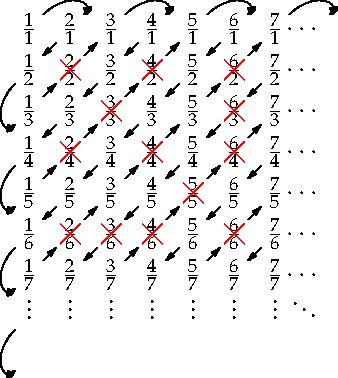
\includegraphics{intro-qcount}
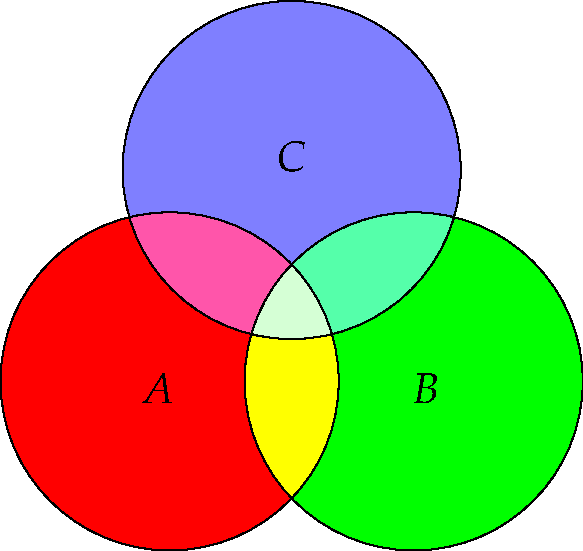
\includegraphics{intro-venndist}
\end{center}

\vfill\vfill\vfill

\clearpage


\pagenumbering{roman}


%\thispagestyle{empty}
\tableofcontents

\clearpage

\section*{Preface: What is Math 13 and who is it for?}
\label{sec:preface}
\addcontentsline{toc}{section}{\nameref{sec:preface}}

Math 13 was created by the late Howard Tucker as a traditional discrete mathematics course, with the number 13 chosen as a joke! It eventually evolved to become the key transition class in UCI's undergraduate program, introducing students to abstraction and proof, and serving as the primary pre-requisite for upper-division courses such as abstract algebra, analysis, linear algebra \& number theory.\smallbreak

The typical student is simultaneously working through lower-division calculus and linear algebra. Knowledge of such material is unnecessary and students are encouraged to take the class early both to ease the transition from algorithmic to abstract mathematics, and so that a proof-mentality may be brought to other lower-division classes.\smallbreak

This text evolved from course notes dating back to 2008. Math 13 is something of a hydra due to the niche it occupies in UCI's program: part proof-writing, part discrete mathematics, and part introduction to specific upper-division topics. Abstract logic is covered only at a basic level while set theory is spread throughout the text; the intent is for such dry `grammar' topics to be absorbed via engagement with more accessible and fun ideas. By the end of the course, interested students should be prepared for a formal study of logic and set theory at the upper-division level.


\boldsubsubsection{Learning Outcomes}

\begin{enumerate}
	\item Developing the skills necessary to read and practice abstract mathematics.
	\item Understanding the concept of proof and becoming acquainted with multiple proof techniques.
	\item Learning what sort of questions mathematicians ask and what excites them.
	\item Introducing upper-division mathematics by providing a taste of what is covered in several courses. For instance:
	\begin{description}
		\item[\normalfont\emph{Number Theory \& Abstract Algebra}] How can we perform arithmetic with remainders? Can you figure out what on which \emph{day} of the week you were born? 
		\item[\normalfont\emph{Geometry and Topology}] How can we visualize and work with objects such as the Möbius strip? How can we use sequences of sets to produce objects (fractals) that appear similar at all scales?
		\item[\normalfont\emph{To Infinity and Beyond!}] Why are some infinities greater than others?
	\end{description}
\end{enumerate}


\boldinline{Useful Texts}

The following texts are recommended if you want more exercises and material. The first two are available free online, while the remainder were previous textbooks for Math 13.

\begin{itemize}%\itemsep0pt
	\item \href{http://www.people.vcu.edu/~rhammack/BookOfProof/}{\emph{Book of Proof}}, Richard Hammack%, %2nd ed 
		%2013.
	
	\item \href{http://scholarworks.gvsu.edu/books/9/}{\emph{Mathematical Reasoning}}, Ted Sundstrom%, %2nd ed 
		%2014.

	\item \emph{Mathematical Proofs: A Transition to Advanced Mathematics}, Chartrand/Polimeni/Zhang%, %3\rd{} Ed
		%2013.%, Pearson.
	\item \emph{The Elements of Advanced Mathematics}, Steven G. Krantz%, %2\nd{} ed 
		%2002.%, Chapman \& Hall.
	\item \emph{Foundations of Higher Mathematics}, Peter Fletcher and C.~Wayne Patty%, %3\rd{} ed
		%2000.%, Brooks--Cole.
\end{itemize}




\clearpage

\iffalse

\subsection*{Notation}
\label{sec:notation}
\addcontentsline{toc}{section}{\nameref{sec:notation}}

Sets of numbers: $\N$, $\N_0$, $\Q$, $\R$


\clearpage

\fi

\pagenumbering{arabic}

\section{Introduction: What is a Proof?}\label{chap:intro}


The essential concept in higher-level mathematics is that of \emph{proof.} A basic dictionary entry might cover two meanings:
\begin{enumerate}%\itemsep0pt
	\item A test or trial of an assertion.
	\item An argument that establishes the validity (truth) of an assertion.
\end{enumerate}
In science and wider culture, the first meaning predominates: a defendant was \emph{proved} guilty in court; a skin cream is clinically \emph{proven} to make you look younger; an experiment \emph{proves} that the gravitational constant is $9.81\mathrm{ms}^{-2}$. A common mistake is to treat such a proved assertion as unambiguously true. Distinct juries might disagree as to whether a defendant is guilty; indeed for many crimes the truth is uncertain, hence the more nuanced legal expression \emph{proved beyond reasonable doubt.}\smallbreak

In mathematics we use the second meaning: a proof establishes the incontrovertible \emph{truth} of some assertion. To see what we mean, consider a simple claim (mathematicians use the word \emph{theorem}).

\begin{thm}{}{sumeven}
	The sum of any pair of even integers is even.
\end{thm}

Hopefully you believe this statement. But how do we \emph{prove} it? We can \emph{test} the assertion by considering \emph{examples} ($4+6=10$ is even, $(-8)+30=22$ is even, etc.), but we cannot expect to verify \emph{all} pairs this way. For a mathematical proof, we somehow need to test all possible examples simultaneously. To do so, it is essential to have a clear idea of what is meant by an \emph{even integer.}

\begin{defn}{}{even}
	An integer is \emph{even} if it may be written in the form $2k$ where $k$ is an integer.
\end{defn}

\begin{proof}
	Let $x$ and $y$ be even. Then $x=2k$ and $y=2l$ for some integers $k$ and $l$. But then
	\[
		x+y=2k+2l=2(k+l)\tag{$\ast$}
	\]
	is even.
\end{proof}

The box \smash{\raisebox{8pt}{$\qedsymbol$}} indicates the end of the argument. Traditionally the letters Q.E.D.{} were used, an acronym for the Latin \emph{quod erat demonstrandum} (\emph{which is what was to be demonstrated}).
\smallbreak

Consider how the proof depends crucially on the definition.

\begin{itemize}\itemsep0pt
	\item The theorem did not mention any \emph{variables,} though these were essential to the proof. The variables $k$ and $l$ come for free \emph{once you write the definition of evenness!} This is very common; simple proofs are often little more than rearranged definitions.
	\item According to the definition, $2k$ and $2l$ together represent \emph{all possible pairs} of even integers. It is essential that $k$ and $l$ be \emph{different symbols}: Is is clear why? What would you be proving if $k=l$? %otherwise all you would be proving is that twice an even number is even!
	\item The calculation ($\ast$) is the easy bit; without the surrounding sentences and the direct reference to the definition of evenness, the calculation means nothing.
\end{itemize}

Notice the sleight of hand: a mathematical proof establishes truth \emph{only} by reference to one or more \emph{definitions}.\footnote{Strictly speaking, the definition and theorem also depend on the meanings of \emph{integer} and \emph{sum,} though to rigorously define either would take us too far afield. In any context, some concepts will be considered too basic to merit definition.}


\goodbreak


\boldsubsection{Theorems \& Conjectures}

Theorems are true mathematical statements that we can prove. Some are important enough to merit names (Pythagorean theorem, fundamental theorem of calculus, rank--nullity theorem, etc.), but most are simple statements such as Theorem \ref{thm:sumeven}.\smallbreak

In practice we are often confronted with \emph{conjectures}: statements we suspect to be true, but which we don't (yet) know how to prove. Much of the fun and creativity of mathematics lies in formulating and attempting to prove (or disprove) conjectures.\smallbreak

A conjecture is the mathematician's analogue of the scientist's hypothesis: a statement one would like to be true. The difference in approach takes us right back to the dual meaning of \emph{proof.} The scientist \emph{tests} their hypothesis using the scientific method, conducting experiments which attempt (and hopefully fail!) to show that the hypothesis is incorrect. The mathematician tries to \emph{prove} the validity of a conjecture by relying on logic. The job of a mathematical researcher is to formulate conjectures, prove them, and publish the resulting theorems. Attempting to formulate your own conjectures is an essential part of learning mathematics; many will likely be false, but you'll learn much by figuring out why!\medbreak

Here are two conjectures to give us a taste of this process.

\begin{conj}{}{n^2-1}
	If $n$ is any odd integer, then $n^2-1$ is a multiple of 8.
\end{conj}

\begin{conj}{}{n^2+n+41}
	If $n$ is any positive integer, then $n^2+n+41$ is prime.\footnotemark
\end{conj}

\footnotetext{\label{fn:introprime}A positive integer is \emph{prime} if it cannot be written as the product of two integers, both greater than one.}

How can we decide if these conjectures are true or false? To get a feel for things, we start by computing examples for several small integers $n$. (In practice, this is likely what lead to the formulation of the conjectures in the first place!)
\[
	\def\arraystretch{1.2}
	\begin{array}{l||c|c|c|c|c|c|c}
		n & 1 & 3 & 5 & 7 & 9 & 11 & 13\\\hline
		n^2-1 & 0 & 8 & 24 & 48 & 80 & 120 & 168
	\end{array}
	\qquad\quad
	\begin{array}{l||c|c|c|c|c|c|c}
		n & 1 & 2 & 3 & 4 & 5 & 6 & 7\\\hline
		n^2+n+41 & 43 & 47 & 53 & 61 & 71 & 83 & 97
	\end{array}
\]
Since 0, 8, 24, 48, 80, 120 and 168 are all multiples of 8, and 43, 47, 53, 61, 71, 83 and 97 are all prime, both conjectures \emph{appear} to be true. Would you bet \$100 that this is indeed the case? Is $n^2-1$ a multiple of 8 for \emph{every} odd integer $n$? Is $n^2+n+41$ prime for \emph{every} positive integer $n$? Establishing whether each conjecture is true or false requires one of the following:

\begin{quote}
\begin{description}
  \item[\normalfont\emph{Prove it}] by showing it must be true in \underline{all} cases, or,
  \item[\normalfont\emph{Disprove it}] by finding \underline{at least one} instance in which the statement is false.
\end{description}
\end{quote}

Let us start with Conjecture \ref{conj:n^2-1}. If $n$ is an odd integer, then, by definition, we may write $n=2k+1$ for some integer $k$. Now compute the object of interest:
\[
	n^2-1 =(2k+1)^2-1 =(4k^2+4k+1)-1 =4k^2+4k =4k(k+1)
\]
We need to investigate whether this is \emph{always} a multiple of 8. Since $k$ is an integer, $n^2-1$ is plainly a multiple of 4, so everything comes down to deciding whether $k(k+1)$ is \emph{always even.} Do we believe this? We return to testing some small values of $k$:
\[
	\def\arraystretch{1.2}
	\begin{array}{l||c|c|c|c|c|c|c}
		k & -2 & -1 & 0 & 1 & 2 & 3 & 4\\\hline
		k(k+1) & 2 & 0 & 0 & 2 & 6 & 12 & 20
	\end{array}
\]
Once again, the claim seems to be true for small values of $k$, but is it is true for \emph{all} $k$? Again, the only way is to \emph{prove} or \emph{disprove it}. Observe that $k(k+1)$ is the \emph{product of two consecutive integers.} This is great, because for any two consecutive integers one is even and the other odd; their product must be even. Conjecture \ref{conj:n^2-1} is indeed a \emph{theorem!}\smallbreak

So far, our approach has been investigative. Scratch work is an essential part of the process, but we shouldn't expect a reader to have to fight their way through such. We therefore offer a \emph{formal proof}. This is the final result of our deliberations; investigate, spot a pattern, conjecture, prove, and finally present our work in as clean and convincing a manner as we can.

\begin{thm}{}{n^2-1}
	If $n$ is any odd integer, then $n^2-1$ is a multiple of 8.
\end{thm}

\begin{proof}
	Let $n$ be an odd integer. By definition, we may write $n=2k+1$ for some integer $k$. Then
	\[
		n^2-1=(2k+1)^2-1=(4k^2+4k+1)-1=4k^2+4k=4k(k+1)
	\]
	We distinguish two cases. If $k$ is even, then $k(k+1)$ is even and so $4k(k+1)$ is divisible by 8.\smallbreak
	If $k$ is odd, then $k+1$ is even. Therefore $k(k+1)$ is again even and $4k(k+1)$ divisible by 8.\smallbreak
	In both cases $n^2-1=4k(k+1)$ is divisible by 8.
\end{proof}

All that work, just for five lines of clean argument! But wasn't it \emph{fun}?\medbreak

When constructing elementary proofs it is common to be unsure over how much detail to include. We relied on the definition of \emph{oddness,} but we also used the fact that a product is even whenever either factor is even; does this need a proof? Since the purpose of a proof is to convince the reader, the appropriateness of an argument will depend on context and your audience: if you are trying to convince a middle-school student, maybe you should justify this step more fully, though the cost would be a longer argument whose totality is harder to grasp. A proof that works perfectly in all situations is unlikely to exist! A good rule is to imagine writing for another mathematician at your own level---if a fellow student believes your argument, that's a good sign of both its validity and appropriateness.
\bigbreak

We now consider Conjecture \ref{conj:n^2+n+41}. The question is whether $n^2+n+41$ is prime for \emph{every} positive integer $n$. When $n\le 7$ the answer is \emph{yes}, but examples do not make a proof! To investigate further, return to the definition of prime (footnote \ref{fn:introprime}): is there a positive integer $n$ for which is $n^2+n+41$ can be factored as a product of two integers, both at least 2? A straightforward answer is staring us in the face! When $n=41$ such a factorization certainly exists:
\[
	n^2+n+41 =41^2+41+41 =41(41+1+1) =41\cdot 43
\]
We call $n=41$ a \emph{counterexample}; there is at least one integer $n$ for which $n^2+n+41$ is \emph{not} prime. Conjecture \ref{conj:n^2+n+41}, being a claim about \emph{all} integers $n$, is therefore \emph{false}---it has been \emph{disproved}.



\boldsubsubsection{Planning and Writing Proofs}
\phantomsection\label{sec:proofplan}

Your main responsibility in this course is the construction of proofs. Their sheer variety means that, unlike in elementary calculus, you cannot simply practice tens of similar problems until the process becomes automatic. So how do you learn to write proofs?\smallbreak

The first step is to \emph{read} other arguments. Don't just accept them, make sure you \emph{believe} them: check the calculations, verify claims, and rewrite the argument in your own words adding any clarifications you deem necessary or helpful.\smallbreak

As you dissect others' work, a daunting question often arises: \emph{how did they ever come up with this?} As our work on Theorem \ref{thm:n^2-1} shows, the source of a proof is often less magical than it appears; usually the author experimented until they found something that worked. The experimentation is hidden in the final proof, whose purpose is to be as clean and convincing as possible. A proof is akin to a concert performance after hours of private practice; wrong notes don't belong in the Carnegie Hall!\smallbreak

In order to bridge the gap, we recommend splitting the proof-writing process into several steps.

\begin{description}
	\item[Interpret] Make sense of the statement. What is it saying? Can you rephrase in a clearer manner? What are you assuming? A key part of this step is identifying the \emph{logical structure} of the statement. We'll discuss this at length in the next chapter.
    
	\item[Brainstorm] Convince \emph{yourself} that the statement is true. First, look up the relevant definitions. Next, think of some instances where the conditions of the statement are met. Try out some examples, and ask yourself what makes the claim work in those instances. Examples can help build intuition about \emph{why} a claim is true and sometimes suggest a proof strategy. Review other theorems that use these definitions. Do you know any theorems that relate your assumptions to the conclusion? Have you seen a proof of a similar statement before?

	\item[Sketch] Build the skeleton of your proof. Think again about what you are assuming and what you are are you trying to prove. It is often straightforward to write down reasonable \emph{first} and \emph{last} steps (the bread slices of a \emph{proof-sandwich}). Try to connect these with informal arguments. If you get stuck, try a different approach.\par
	This step is often the longest in the proof-writing process. It is also where you will be doing most of your calculations. You can be as messy as you like because \emph{no-one ever has to see it}! Once you've learned a variety of proof methods, this is a good stage at which to experiment with different approaches.
  
	\item[Prove] Once you have a suitable sketch, it's time to prove the statement to the world. Translate your sketch into a linear story. Carefully word your explanations and avoid shorthand, though well-understood mathematical symbols such as $\Longrightarrow$ are encouraged. The result should be a clear, formal proof such as you'd find in a mathematics textbook. Although you are providing a mathematical argument, your proof should read like prose and be written in \emph{complete sentences}. 

	\item[Review] Finally, review your proof. Assume the reader is meeting the problem for the first time and has not seen your sketch. Read your proof with skepticism; consider its readability and flow. Get rid of unnecessary claims and revise the wording if necessary. Read your proof out loud. If you're adding extra words that aren't written down, include them in the proof. Share your work with others. Do they understand it \emph{without any additional input from you}?
\end{description}

\goodbreak



\boldsubsubsection{Conjectures: \emph{True} or \emph{False}?}

Higher-level mathematics is all about the links between proofs, definitions, theorems and conjectures. We prove theorems (and solve homework problems) because they make us use, and aid our understanding of, definitions. We state definitions to help us formulate conjectures and prove theorems. One does not \emph{know} mathematics, one \emph{does} it. Mathematics is a \emph{practice}; an art as much as it is a science.\medbreak

With this in mind, do your best to prove or disprove the following conjectures. Don't worry if some terms or notations are unfamiliar: ask! Everything will be covered formally soon enough. At the end of the course, revisit these problems to realize how much your proof skills have improved. 

\begin{enumerate}
	\item The sum of any three consecutive integers is even.
	\item There exist integers $m$ and $n$ such that $7m+5n =4$.
	\item Every common multiple of 6 and 10 is divisible by 60.
	\item There are integers $x$ and $y$ which satisfy $6x+9y =10$.
	\item For every positive real number $x$, the value $x+\frac 1x$ is greater than or equal to 2.
	\item If $x$ is any real number, then $x^2\ge x$.
	\item If $n$ is an integer, then $n^2+5n$ must be even.
	\item If $x$ is a real number, then $\nm x\ge -x$.
	\item If $n$ is an integer greater than 2, then $n^2-1$ is not prime.
	\item An integer is divisible by 5 whenever its last digit is 5.
	\item If $r$ is a rational number, then there is a non-zero integer $n$ such that $rn$ is an integer.
	\item There is a smallest positive real number.
	\item For all real numbers $x$, there exists a real number $y$ for which $x<y$.
	\item There is a real number $x$ such that, for all real numbers $y$, we have $x<y$.
	\item The sets $A=\{n\in\N:n^2<25\}$ and $B=\{n^2:n\in\N\text{ and }n<5\}$ are equal. Here $\N$ denotes the set of natural numbers.
\end{enumerate}




\section{Logic and the Language of Proofs}\label{sec:logic}


\subsection{Propositions}\label{sec:prop}


In order to read and construct proofs, we need to start with the language in which they are written: \emph{logic.} This is to mathematics what grammar is to English.


\begin{defn}{}{}
	A \emph{proposition} or \emph{statement} is a sentence that is either true or false.
\end{defn}

\begin{examples}{}{}
\exstart $17-24=7$. \hfill \makebox[250pt][l]{2. \ $39^2$ is an odd integer.\hfill}\vspace{-3pt}
	\begin{enumerate}\setcounter{enumi}{2}\itemsep0pt
		\item The moon is made of cheese. \hfill \makebox[250pt][l]{4. \ Every cloud has a silver lining.\hfill} 
		\setcounter{enumi}{4} 
		\item God exists.
	\end{enumerate}
\end{examples}

For a proposition to make sense, we must agree on the meaning of each concept it contains. When people argue over propositions, in practice they are often disagreeing about \emph{definitions.} There are many concepts of God; we cannot begin to consider whether or not They exist until we agree \emph{which} concept is being discussed! This also illustrates that the truth status of a proposition \emph{need not be known} at the moment you state it; this is particularly common in mathematics.\footnote{More surprisingly, there are even propositions whose truth state is impossible to determine!}



\boldsubsubsection{Truth Tables and Combining Propositions}

To develop basic rules and terminology, it is helpful to consider \emph{abstract} propositions: $P,Q,R,\ldots$. Given a small number of propositions, all possible combinations of truth states may be easily represented in tabular format: in a \emph{truth table.} These are useful for defining new propositions.

\begin{defn}{}{}
	Let $P$ and $Q$ be propositions. The truth tables below define three new propositions modeled on the words \emph{and, or} and \emph{not.}\par
	\begin{minipage}[t]{0.5\linewidth}\vspace{0pt}
		\begin{itemize}
		  \item The \emph{conjunction} $\textcolor{red}{P\wedge Q}$ is read ``$P$ and $Q$.''
		  \item The \emph{disjunction} $\textcolor{Green}{P\vee Q}$ is read ``$P$ or $Q$.''
		  \item The \emph{negation} $\textcolor{blue}{\neg P}$ is read ``not $P$.'' %or \emph{denial} (NOT, $\neg$, $\sim$, $\cl{\phantom{P}}$)
		\end{itemize} 
	\end{minipage}
	\hfill
	\begin{minipage}[t]{0.49\linewidth}\vspace{-2pt}
		$\begin{array}{cc||c|c}
			P & Q & \textcolor{red}{P\wedge Q} & \textcolor{Green}{P\vee Q}\\\hline
			T & T & \textcolor{red}{T} & \textcolor{Green}{T}\\
			T & F & \textcolor{red}{F} & \textcolor{Green}{T}\\
			F & T & \textcolor{red}{F} & \textcolor{Green}{T}\\
			F & F & \textcolor{red}{F} & \textcolor{Green}{F}
		\end{array}
		\qquad\qquad
		\begin{array}[b]{c||c}
			P & \textcolor{blue}{\neg P}\\\hline
			T & \textcolor{blue}{F}\\
			F & \textcolor{blue}{T}
		\end{array}$
	\end{minipage}
\end{defn}

The letters T/F stand for \emph{true/false.} E.g., the second line of the first table says that if $P$ is true and $Q$ is false, then the proposition ``$P$ and $Q$" is \textcolor{red}{false}, while ``$P$ or `$Q$'' is \textcolor{Green}{true.} %Hopefully this gels with your intuitive understanding.

\begin{example}{}{logiccolor}
	Suppose $P$ and $Q$ are the following propositions:
	\begin{quote}
		$P$: ``I like purple.''\qquad\qquad $Q$: ``I like chartreuse.''
	\end{quote}
	We form the new propositions described in the definition:
	\begin{quote}
		$P\wedge Q$: ``I like purple and chartreuse.''\qquad \qquad
		$P\vee Q$: ``I like purple or chartreuse.''\smallbreak
		$\neg P$: ``I do not like purple.''
	\end{quote}
	It is typical to modify phrasing to aid readability: ``Not, I like purple'' just sounds weird! Note also that or is \emph{inclusive} in logic: if ``I like purple or chartreuse'' is true, then you might like \emph{both}!\medbreak
	
	Let's continue by adding a third proposition:
	\begin{quote}
		$R$: ``It's 9am.''
	\end{quote}
	What proposition is represented by the following English sentence?
	\begin{quote}
		``I like purple and I like chartreuse or it's 9am.''
	\end{quote}
	Is it $P\wedge(Q\vee R)$ or is it $(P\wedge Q)\vee R$? Without brackets, the sentence is unclear; the moral is that English is terrible at logic! Indeed, as the truth table shows, the two logical expressions \textcolor{red}{really do mean different things!}\vspace{-1pt}
	 \[
	 \begin{array}{ccc||cc||cc}
			P & Q & R & Q\vee R & P\wedge (Q\vee R) & P\wedge Q & (P \wedge Q)\vee R\\\hline
			T & T & T & T & T & T & T\\
			T & T & F & T & T & T & T\\
			T & F & T & T & T & F & T\\
			T & F & F & F & F & F & F\\
			F & T & T & T & \textcolor{red}{F} & F & \textcolor{red}{T}\\
			F & T & F & T & F & F & F\\
			F & F & T & T & \textcolor{red}{F} & F & \textcolor{red}{T}\\
			F & F & F & F & F & F & F
		\end{array}
	 \]
\end{example}


\boldsubsubsection{Conditional and Biconditional Connectives}

Of critical importance is the ability to have one proposition lead to another.

\begin{defn}[lower separated=false, sidebyside, sidebyside align=top seam, sidebyside gap=0pt, righthand width=0.37\linewidth]{}{implies}
	Given propositions $P,Q$, the \emph{conditional} ($\Longrightarrow$) and \emph{biconditional} ($\Longleftrightarrow$) \emph{connectives} define new propositions as described in the truth table.\smallbreak
	For the proposition $P\Longrightarrow Q$, we call $P$ the \emph{hypothesis} and $Q$ the \emph{conclusion.}
	\tcblower
	\flushright$\begin{array}{cc||c|c}
	P & Q & P\implies Q & P\iff Q\\\hline
	T & T & T & T\\
	T & F & F & F\\
	F & T & T & F\\
	F & F & T & T
	\end{array}$
\end{defn}


%Remember that the expressions $P\Longrightarrow Q$ and $P\Longleftrightarrow Q$ are themselves \emph{propositions}: sentences which are either true or false. 
Connective propositions can be read and written in many different ways:
\begin{quote}
	\def\arraystretch{1.05}
	\begin{tabular}{@{}cc|c}
		\multicolumn{2}{c|}{$P\implies Q$} & $P\iff Q$\\\hline
		$P$ implies $Q$ & $P$ therefore $Q$ & $P$ if and only if $Q$\\
		If $P$, then $Q$ & $Q$ follows from $P$ & $P$ iff $Q$\\
		$P$ only if $Q$ & $Q$ if $P$ & $P$ and $Q$ are (logically) equivalent\\
		$P$ is sufficient for $Q$ & $Q$ is necessary for $P$ & $P$ is necessary and sufficient for $Q$
	\end{tabular}
\end{quote}


\begin{example}{}{}
	The following sentences express, in English, the same conditional $P\implies Q$.\vspace{-1pt}
	\begin{itemize}\itemsep1pt
		\item If you are born in Rome, then you are Italian. 
		\item You are Italian if you are born in Rome. 
		\item You are born in Rome only if you are Italian. 
		\item Being born in Rome is sufficient for being Italian. 
		\item Being Italian is necessary for being born in Rome.\vspace{-1pt} 
	\end{itemize}
	Are you comfortable with what the propositions $P$ and $Q$ are here?
\end{example}

%\goodbreak

Connectives are central to mathematics for many reasons. In particular:
\begin{enumerate}
  \item The vast majority of theorems we'll encounter may be written as a connective $P\Longrightarrow Q$. For instance, revisit Theorem \ref{thm:sumeven} and the discussion that follows:
  \begin{quote}
  	If $x$ and $y$ are even integers, then $x+y$ is even.
  \end{quote}
  Identifying the hypothesis and conclusion is essential if you want to understand a theorem!
  \item Simple proofs typically involve chaining a sequence of connectives:
  \[P\implies P_2\implies \cdots \implies P_n\implies Q\]
\end{enumerate}
We'll revisit these ideas in Section \ref{sec:proof}, and repeatedly throughout the course.\bigbreak


While the biconditional should be easy to remember, %($P\Longleftrightarrow Q$ is true precisely when $P$ and $Q$ have identical truth states)
it is harder to make sense of the conditional connective. Short of simply memorizing the truth table, here are two examples that might help.

\begin{examples}{}{condmeaning}
	\exstart Suppose your professor says, ``If the class earns a B average on the midterm, then I'll bring doughnuts.'' The only situation in which the teacher will have lied is if the class earns a B average but she fails to provide doughnuts.
	\begin{enumerate}\setcounter{enumi}{1}
	  \item ($F\Longrightarrow T$ really can be true!) Let $P$ be the proposition ``$7=3$'' and $Q$ be ``$0=0$.'' Since multiplication of both sides of an equation by zero is algebraically valid, we see that
	%   \[7=3\implies 0\cdot 7=0\cdot 3\implies 0=0\]
	  \begin{align*}
			7=3\implies\ &0\cdot 7=0\cdot 3\tag*{(If $7=3$, then 0 times 7 equals 0 times 3)}\\
			\implies\ &0=0\tag*{(then 0 equals 0)}
		\end{align*}
	  This argument is perfectly correct: the \emph{implication} $P\Longrightarrow Q$ is \emph{true.} It (rightly!) makes us uncomfortable because the hypothesis is \emph{false.}\par
	  If we instead add 1 to each side of $7=3$, we'd obtain a example where $F\Longrightarrow F$ is true.
	\end{enumerate}
\end{examples}


\boldsubsubsection{Tautologies and Contradictions}

\begin{defn}{}{tautology}
	A \emph{tautology} is a logical expression that is always true, regardless of what the component statements might be.\smallbreak
	A \emph{contradiction} is a logical expression that is always false.
\end{defn}

%The easiest way to detect these is to construct a truth table.

\begin{examples}{}{}
\exstart $P\wedge(\neg P)$ is a contradiction.
	
\begin{enumerate}\setcounter{enumi}{1}
  \begin{minipage}[t]{0.65\linewidth}\vspace{-8pt}
  	\item[] Regardless of the proposition $P$, it cannot be true at the same time as its negation!
  \end{minipage}
  \hfill
  \begin{minipage}[t]{0.29\linewidth}\vspace{-27pt}
	$\begin{array}{cc|c}
	P & \neg P & P\wedge(\neg P)\\\hline
	T & F & F\\
	F & T & F
	\end{array}$
  \end{minipage}\par
  
	\item $\bigl(P\wedge(P\implies Q)\bigr)\Longrightarrow Q$ is a tautology.% This is essentially how we understand a direct proof: if $P$ is true and we have a correct argument $P\implies Q$, then $Q$ must also be true.
	\[\begin{array}{cc||c|c||c}
	P & Q & P\implies Q & P\wedge(P\implies Q) & \bigl(P\wedge(P\implies Q)\bigr)\implies Q\\\hline
	T & T & T & T& T\\
	T & F & F & F& T\\
	F & T & T & F& T\\
	F & F & T & F& T
	\end{array}\]
	%\item $(P\wedge \neg Q\implies F)\iff (P\implies Q)$ is a tautology. This tautology is the basis for \emph{proof by contradiction,} as we'll see in the next section. The expression $P\wedge \neg Q\implies F$ can be thought of as saying that $P\wedge\neg Q$ implies a contradiction.
	\end{enumerate}
\end{examples}

\goodbreak


\boldsubsubsection{The Converse and Contrapositive}

%The following constructions are used regularly; it is vitally important to understand the distinction.

\begin{defn}{}{contra}
	The \emph{converse} of $P\Longrightarrow Q$ is the reversed implication $Q\Longrightarrow P$.\smallbreak
	The \emph{contrapositive} of $P\Longrightarrow Q$ is the implication $\neg Q\Longrightarrow\neg P$.
\end{defn}

It is vital to understand the distinction between these. In general, the truth status of the converse bears no relation to that of the original, though the contrapositive is much better behaved.

\begin{thm}{}{contrapos}
	The contrapositive of an implication is logically equivalent to the original.
\end{thm}

\begin{proof}
	Compute the truth table and observe that the third and sixth columns are identical:\footnotemark
	\begin{gather*}
		\begin{array}{cc|c||cc|c}
			P & Q & P\Longrightarrow Q & \neg Q & \neg P & \neg Q\Longrightarrow\neg P\\\hline
			T & T & T & F & F & T\\
			T & F & F & T & F & F\\
			F & T & T & F & T & T\\
			F & F & T & T & T & T
		\end{array}\\[-15pt]
		\phantom{bob}\tag*{\qedhere}
	\end{gather*}
	%Otherwise said, $(P\Longrightarrow Q)\Longleftrightarrow (\neg Q\Longrightarrow\neg P)$ is a tautology.
\end{proof}

\footnotetext{Otherwise said, $(P\Longrightarrow Q)\Longleftrightarrow (\neg Q\Longrightarrow\neg P)$ is a tautology.}

\vspace{-5pt}


\begin{example}{}{}
	Let $P$ and $Q$ be the following statements:
	\begin{quote}
	  $P$: \ ``Claudia is holding a peach.''\qquad\qquad
	  $Q$: \ ``Claudia is holding a piece of fruit.''
	\end{quote}
	Since a peach is indeed a piece of fruit, the proposition $P\Longrightarrow Q$ is \emph{true}:
	\begin{quote}
		$P\Longrightarrow Q$: \ ``If Claudia is holding a peach, then she is holding a piece of fruit.''
	\end{quote}
	The \emph{converse} of $P\Longrightarrow Q$ is the sentence
	\begin{quote}
	  $Q\Longrightarrow P$: \ ``If Claudia is holding a piece of fruit, then she is holding a peach.''
	\end{quote}
	This is palpably false: Claudia could be holding an apple! However, in accordance with Theorem \ref{thm:contrapos}, the \emph{contrapositive} is \emph{true}:
	\begin{quote}
	  $\neg Q\Longrightarrow \neg P$: ``If Claudia is \emph{not} holding any fruit, then she is \emph{not} holding a peach.''
	\end{quote} 
\end{example}

 
\boldsubsubsection{Negating Logical Expressions}

Mathematics often requires us to negate propositions. What would you suspect to be the negation of a conditional $P\Longrightarrow Q$? Is it enough to say ``$P$ doesn't imply $Q$"? But what does this mean? 

\begin{minipage}[t]{0.64\linewidth}\vspace{-2pt}
We again rely on a truth table: to get the last column, recall that negation simply swaps $T$ and $F$. Can we write this column in another way? Since there is only a single $T$ in the final column, we see that we've proved the following.
\end{minipage}
\hfill
\begin{minipage}[t]{0.35\linewidth}\vspace{-5pt}
\flushright $\begin{array}{cc|c|c}
		P & Q & P\Longrightarrow Q & \neg(P\Longrightarrow Q)\\\hline
		T & T & T & F\\
		T & F & F & T\\
		F & T & T & F\\
		F & F & T & F
	\end{array}$
\end{minipage}



\begin{thm}{}{negconditional}
	$\neg(P\Longrightarrow Q)$ is logically equivalent to $P\wedge\neg Q$ \ (``$P$ and not $Q$").
\end{thm}

\vspace{-5pt}

\goodbreak

\begin{example}{}{}
	Consider the implication
	\begin{quote}
	  It's the morning therefore I'll have coffee.
	\end{quote}
	Hopefully its negation is clear:
	\begin{quote}
	  It's the morning \emph{and} I \emph{won't} have coffee.
	\end{quote}
	As in Example \ref{ex:condmeaning}, it might help to think about what it means for the original statement to be \emph{false}.
\end{example}

\begin{tcolorbox}
{\bf \textcolor{red}{Warning!}} The negation of $P\Longrightarrow Q$ is \emph{not a conditional.} In particular it is \emph{neither} of the following:
\begin{quote}
  The converse $Q\Longrightarrow P$.\smallbreak
  The contrapositive of the converse $\neg P\Longrightarrow\neg Q$. 
\end{quote}
If you are unsure about this, write down the truth tables and compare.
\end{tcolorbox}

\bigbreak


Our final results in basic logic also involve negations; they are named for Augustus de Morgan, a famous 19\th{} century logician.

\begin{thm}{de Morgan's laws}{demorgan}
	Let $P$ and $Q$ be propositions.
	\begin{enumerate}\itemsep0pt
	  \item $\neg(P\wedge Q)$ is logically equivalent to $\neg P\vee\neg Q$
	  \item $\neg(P\vee Q)$ is logically equivalent to $\neg P\wedge\neg Q$
	\end{enumerate}
\end{thm}

\begin{proof}
	For the first law, observe that the fourth and seventh columns of the truth table are identical.
	\[
		\begin{array}[t]{cc||cc||cc||c}
			P & Q & P\wedge Q & \neg(P\wedge Q) & \neg P & \neg Q & \neg P\vee\neg Q\\\hline
			T & T & T & F & F & F & F\\
			T & F & F & T & F & T & T\\
			F & T & F & T & T & F & T\\
			F & F & F & T & T & T & T
		\end{array}
	\]
	The second law is an exercise.
\end{proof}

\begin{example}{}{}
	Consider the sentence:\par
	\begin{minipage}[t]{0.6\linewidth}\vspace{-1pt}
	\begin{quote}
		I rode the subway \emph{and} I had coffee.
	\end{quote}
	To negate this using de Morgan's first law, we might write:
	\begin{quote}
		I \emph{didn't} ride the subway \emph{or} I \emph{didn't} have coffee.
	\end{quote}
	\end{minipage}
	\hfill
	\begin{minipage}[t]{0.39\linewidth}\vspace{-20pt}
		\flushright	
		\begin{tabular}{c|c||c}
			Subway&Coffee&Su and Co\\\hline\hline
			T & T & T\\
			\textcolor{blue}{T} & \textcolor{blue}{F} & \textcolor{blue}{F}\\
			\textcolor{blue}{F} & \textcolor{blue}{T} & \textcolor{blue}{F}\\
			\textcolor{blue}{F} & \textcolor{blue}{F} &\textcolor{blue}{F}
		\end{tabular}
	\end{minipage}\bigbreak
	
	This feels awkward in English because the negation encompasses \textcolor{blue}{three distinct possibilities}. Note how the logical (inclusive) use of \emph{or} includes the last row of the truth table: the possibility that you neither rode the subway nor had coffee.
\end{example}

As with Example \ref{ex:logiccolor}, this is another advert for the use of logic: English simply isn't very helpful for precisely stating complex logical statements.


\begin{aside}{}{}
\boldinline{Aside: Algebraic Logic}\phantomsection\label{pg:asidelogicalgebra}

%Similarly to de Morgan's laws, 
We can use truth tables to establish other laws of basic logic, for instance:
\[
	\def\arraystretch{1.2}
	\begin{array}{@{}lll@{}}
	\text{Double negation} & \neg(\neg P)\iff P &\\
	\text{Commutativity} & P\wedge Q\iff Q\wedge P & P\vee Q\iff Q\vee P\\
	\text{Associativity} & (P\wedge Q)\wedge R\iff P\wedge(Q\wedge R) & (P\vee Q)\vee R\iff P\vee(Q\vee R)\\
	\text{Distributivity}&(P\wedge Q)\vee R\iff (P\vee R)\wedge (Q\vee R) & (P\vee Q)\wedge R\iff (P\wedge R)\vee (Q\wedge R)
	\end{array}
\]
To make things more algebraic, we've replaced ``is logically equivalent to" with a biconditional.\footnotemark{}\smallbreak

Armed with such laws, one can often suitably manipulate logical expressions without laboriously creating truth tables. This is not the focus of this course, though you might find it fun!\smallbreak

For this course, it is probably not worth memorizing these laws. Your intuitive understanding of \emph{and, or} and \emph{not} mean you'll likely apply the laws correctly whenever necessary.
\end{aside}

\footnotetext{Stating the laws in this fashion is to assert that each expression is a tautology (Definition \ref{defn:tautology}). For instance, to claim that ``$\neg(\neg P)$ is logically equivalent to $P$'' is to assert that $\neg(\neg P)\iff P$ is a tautology.}

\goodbreak

\begin{exercises}{}{}
	A reading quiz and several questions with linked video solutions can be found \href{http://www.math.uci.edu/~ndonalds/math13/selftest/2-1-props.html}{online}.


	\begin{enumerate}
	  \item Express each statement in the form, ``If $\dots$, then $\dots$'' There are many possible correct answers.
			\begin{enumerate}
		  	\item You must eat your dinner if you want to grow.
		  	\item Being a multiple of 12 is a sufficient condition for a number to be even.
		  	\item It is necessary for you to pass your exams in order for you to obtain a degree. 
		  	\item A triangle is equilateral only if all its sides have the same length.
			\end{enumerate}
		
	
	  \item Suppose ``$x$ is an even integer'' and ``$y$ is an irrational number'' are true statements, and that ``$z\geq 3$'' is a false statement. Which of the following are true?\par
	  (\emph{Hint: Label each statement and think about each using connectives})
			\begin{enumerate}
		  	\item If $x$ is an even integer, then $z\geq 3$.
		  	\item If $z\geq 3$, then $y$ is an irrational number.
		  	\item If $z\geq 3$ or $x$ is an even integer, then $y$ is an irrational number.
		  	\item If $y$ is an irrational number and $x$ is an even integer, then $z\geq 3$.
			\end{enumerate}


	  \item Orange County is considering two competing transport plans: widening the 405 freeway and constructing light rail down its median. A local politician is asked, ``Would you like to see the 405 widened or would you like to see light rail?'' The politician wants to sound positive, but to avoid being tied to one project. What is their response?\par
	  (\emph{Hint: Think about how the word `OR' is used in logic})
  
  
	  \item Consider the proposition: ``If the integer $m$ is greater than 3, then $2m$ is not prime.''
	  \begin{enumerate}
	    \item Rewrite the proposition using the word `necessary.'
	 		\item Rewrite the proposition using the word  `sufficient.'
	 		\item Write the negation, converse and contrapositive of the proposition. 
	  \end{enumerate}
	  

  \item Suppose the following sentence is true: ``If Amy likes art, then no-one likes history." What, if anything, can we conclude if we discover that someone likes history.
  
  
  \goodbreak
	  
	  
	  \item Construct the truth tables for the propositions $P\vee(Q\wedge R)$ and $(P\vee Q)\wedge R$. Are they the same?
   
   
  \goodbreak
  
	\item Use truth tables to establish the following laws of logic:
	\begin{enumerate}
	  \item Double negation: \lstsp $\neg(\neg P)\iff P$.
	  \item Idempotent law: \lstsp $P\wedge P\iff P$.
	  \item Absorption law: \lstsp $P\wedge(P\vee Q)\iff P$.
	  \item Distributive law: \lstsp $(P\wedge Q)\vee R\iff (P\vee R)\wedge(Q\vee R)$.
	\end{enumerate}
  
  
  \item\begin{enumerate}
    \item Decide whether $(P\wedge \neg P) \Longrightarrow Q$ is a tautology, a contradiction, or neither.
    \item Explain why $\neg P \vee \neg Q$ is logically equivalent to $P \Longrightarrow (P \wedge\neg Q)$.
    \item Prove: $\bigl((P\wedge \neg Q)\Longrightarrow F\bigr)\Longleftrightarrow  (P\Longrightarrow Q)$ is a tautology. Here $F$ represents a \emph{contradiction.}
  \end{enumerate}
  
  
  \item\begin{enumerate}
    \item Prove that the expressions $(P\Longrightarrow Q)\wedge (Q\Longrightarrow P)$ and $P\Longleftrightarrow Q$ are logically equivalent.
    \item Prove that $\bigl((P\Longrightarrow Q)\wedge (Q\Longrightarrow R)\bigr)\Longrightarrow \bigl(P\Longrightarrow R\bigr)$ is a tautology.
  \end{enumerate}
  Why do these make intuitive sense?

  
  \item Use logical algebra (e.g., page \pageref{pg:asidelogicalgebra}) to show that $\bigl((P\vee Q)\wedge \neg P\bigr)\wedge\neg Q$ is a contradiction.

	
  \item Do there exist propositions $P,Q$ for which both $P\Longrightarrow Q$ and its converse are \emph{false}? Explain.
  
    
	\item Your friend insists that the negation of the sentence ``Mark and Mary have the same height'' is ``Mark or Mary do not have the same height.'' What is the correct negation? Where did your friend go wrong?

		
	\item Suppose that the following statements are \emph{true}:
  \begin{enumerate}
    \item Every octagon is magical. 
    \item If a polygon is not a rectangle, then is it not a square. 
    \item A polygon is a square, if it is magical.
  \end{enumerate}
  Is it true that ``Octagons are rectangles"? Explain your answer.\par
  (\emph{Hint: try rewriting each of the statements as an implication})
  

	\item The connective $\downarrow$ (the \emph{Quine dagger}, \emph{NOR}) is defined by the truth table:\par
	\begin{enumerate}
	\begin{minipage}[t]{0.75\linewidth}\vspace{0pt}
      \item Prove that $P\downarrow Q$ is logically equivalent to $\neg (P\vee Q)$. 
      \item Find a logical expression built using only $P$ and the connective $\downarrow$ which is logically equivalent to $\neg P$.
	\end{minipage}
	\hfill
	\begin{minipage}[t]{0.24\linewidth}\vspace{-25pt}
	\flushright$  \begin{array}{cc|c}
		P & Q & P \downarrow Q\\\hline
		T & T & F\\
		T & F & F\\
		F & T & F\\
		F & F & T
	\end{array}$
	\end{minipage}
	
		\item Find an expression built using only $P$, $Q$ and $\downarrow$ which is logically equivalent to $P\wedge Q$.
  \end{enumerate}
  
\end{enumerate}

\end{exercises}

\clearpage



\subsection{Propositional Functions \& Quantifiers}\label{sec:quant}

The majority of mathematical propositions are more complicated that those seen in Section \ref{sec:prop}. In particular, they typically involve \emph{variables,} for instance
\begin{quote}
	``$x$ is an integer greater than 5.''
\end{quote}

\begin{defn}{}{}
	A \emph{propositional function} is a family of propositions which depend on one or more variables. The collection of permitted variables is the \emph{domain.}
\end{defn}

If $P$ is a propositional function depending on a single variable $x$, then for each object $a$ in the domain, $P(a)$ is a proposition. Typically $P(x)$ is true for some $x$ and false for others.

\begin{example}{}{easyquantprop}
	Consider the propositional function $P(x)$: ``$x^2>4$" with domain the real numbers. Plainly $P(1)$ is false (``$1^2>4$'') and $P(6)$ is true (''$6^2>4$'').
% 	\begin{itemize}
% 	  \item $P(-1)$ is false: it is the sentence ``$(-1)^2>4$.''
% 	  \item $P(6)$ is true: it is the sentence ``$6^2>4$.''
% 	\end{itemize}
\end{example}

%\boldsubsubsection{Quantified Propositions}

In mathematics, propositional functions are often \emph{quantified.} English contains various quantifiers (\emph{all, some, many, few, several,} etc.), but in mathematics we are primarily concerned with just two.


\begin{defn}{}{quant}
	The \emph{universal quantifier} $\forall$ is read `for all'. The \emph{existential quantifier} $\exists$ is read `there exists.' Given a propositional function $P(x)$, we define two new \emph{quantified propositions}:
	\begin{itemize}
	  \item ``$\forall x, P(x)$'' is true if and only if $P(x)$ is true for \emph{every} $x$ in its domain.
	  \item ``$\exists x, P(x)$'' is true if and only if $P(x)$ is true for \emph{at least one} $x$ in its domain.
	\end{itemize}
	It is common to describe the domain when quantifying propositions by including a descriptor after the quantifier (\emph{bounding the quantifier}---see below).
\end{defn}

As with connectives, there are many ways to express quantified propositions both mathematically and in English. The use of symbolic quantifiers involves a trade-off: compact statements can improve clarity, but they are harder to read for the uninitiated, so consider your audience! While it is your choice whether to employ symbolic quantifiers in your own \emph{writing,} it is essential that you know how to \emph{read/recognize} them and that you can \emph{translate} between various incarnations.

\begin{example*}{\ref{ex:easyquantprop} cont.}{}
	To gain some practice with bounded quantifiers, we introduce the notation $x\in\R$: this means that $x$ is a real number.%\footnotemark{} 
	\begin{itemize}
	  \item ``$\forall x\in\R,\ x^2>4$'' might be read, ``The square of every real number is greater than 4.''\par
	  The quantified expression is \emph{false} since $1^2>4$ is false: we call $x=1$ a \emph{counter-example.}
	  \item ``$\exists x\in\R,\ x^2>4$'' might be read, ``There is a real number whose square is greater than 4.''\par
	  The quantified expression is \emph{true} since $6^2>4$ (is true): we call $x=6$ an \emph{example.}
	\end{itemize}
\end{example*}

Due to their importance, it is worth defining these last concepts formally.

\begin{defn}{}{}
	An \emph{example} of $\exists x, P(x)$ is an element $x_0$ in the domain of $P$ for which $P(x_0)$ is \emph{true.}\smallbreak
	A \emph{counter-example} to $\forall x, P(x)$ is an element $x_0$ in the domain of $P$ for which $P(x_0)$ is \emph{false.}
\end{defn}


\goodbreak


% \boldinline{Must I always use all these symbols?}
% 
% Absolutely not! Though you do have to be able to \emph{read} and \emph{understand} them. Remember that the purpose of writing mathematics is to \emph{convince the reader}; your chosen presentation style will have a huge impact on whether you succeed! Here are three presentations based on the previous example:
% \begin{quote}\def\arraystretch{1.2}
% 	\begin{tabular}{l|l}
% 		Pure English & There is a real number whose square is greater than four\\\hline
% 		Pure Logic & $\exists x\in\R, x^2>4$\\\hline
% 		Hybrid & $\exists x\in\R$ such that $x^2>4$
% 	\end{tabular}
% \end{quote}
% There are benefits and drawbacks to all three approaches; each might be entirely appropriate depending on the audiences. In these notes we'll typically follow a hybrid approach, aiming to replace words with symbols when it improves clarity while preserving readability.



\boldinline{Universal Quantifiers and Connectives: Hidden Quantifiers}

Universally quantified statements are interchangeable with implications. Given a propositional function $Q(x)$, let $P(x)$ be the proposition ``$x$ lies in the domain of $Q$." Then
\[
	\tcbhighmath{\text{$\textcolor{blue}{\forall x,Q(x)}$ is logically equivalent to $\textcolor{Magenta}{P(x)\Longrightarrow Q(x)}$}}
\]
\textcolor{Magenta}{Connectives containing variables} are therefore assumed to be \textcolor{blue}{universal}. When written as a connective, the universal quantifier is typically \emph{hidden.}\footnote{By contrast, the existential quantifier is never hidden: it is always explicitly written as a symbol ($\exists$), or as a phrase in English (\emph{there is, there exists, some, at least one,} etc.).}

\begin{examples}{}{oddsquared}
	\exstart The universal statement ``Every cat is neurotic,'' may also be written
	\begin{enumerate}\setcounter{enumi}{1}
	  \item[]\begin{quote}
			If $x$ is a cat, then $x$ is neurotic.
		\end{quote} 
		
		\item Revisiting Example \ref{ex:easyquantprop}, we could rewrite ``$\forall x\in\R, x^2>4$'' as a connective
		\[
			x\in\R\Longrightarrow x^2>4 \tag{If $x$ is a real number, then $x^2>4$}
		\]
		
	  \item\label{ex:oddsquared2} The following three sentences have identical meaning:
	  \begin{quote}
	  	The square of an odd integer is odd.\qquad $\forall n$ odd, $n^2$ is odd.\qquad $n$ odd $\Longrightarrow n^2$ odd.
	  \end{quote}
	  In only one of the sentences is the universal quantifier explicit. For even more variety, the third sentence can also be viewed as a universal statement about all \emph{integers}; including the \textcolor{red}{hidden quantifier} in this case results in
		\[
			\textcolor{red}{\forall n\in\Z},\ n\text{ odd} \implies n^2 \text{ odd.}
		\]
		where the symbol $\Z$ represents the (set of) integers.
	\end{enumerate}
\end{examples}

We've already seen that \emph{disproving} a universal statement requires only that we supply a \emph{counter-example.} While such might require some effort to find, often the resulting argument is very simple. By contrast, \emph{proving} a universal statement is the same as proving a connective, an activity that is typically much more involved. We therefore largely postpone this to the next section. Regardless, a simple proof of our \emph{oddness} claim should be easy to follow.

\begin{proof}[Proof of Example \ref*{ex:oddsquared}.\ref{ex:oddsquared2}]
	If an integer $n$ is odd, then it may be written in the form $n=2k+1$ for some integer $k$. But then
	\[
		n^2 =(2k+1)^2 =4k^2+4k+1 =2(2k^2+2k)+1
		\]
	is plainly also odd.
\end{proof}

Similarly, \emph{proving} an existential statement (by providing an \emph{example}) is typically more straightforward than \emph{disproving} such. To understand this duality, we need to understand how to \emph{negate} quantified propositions.

\goodbreak


\boldsubsubsection{Negating Quantified Propositions}

To negate a proposition, we consider what it means for it to be \emph{false.} We already understand what this means for a universal proposition:
\begin{quote}
	``$\forall x,P(x)$'' is false if and only if \emph{there exists a counter-example.}
\end{quote}
The negation of a universal statement is \emph{existentially quantified}:
\begin{quote}
	The negation of ``$P(x)$ is \emph{always} true'' is ``$P(x)$ is \emph{sometimes} false.''
\end{quote}
Repeating this with $\neg P(x)$ results in a related observation:
\begin{quote}
	The negation of ``$P(x)$ is \emph{always} false" is ``$P(x)$ is \emph{sometimes} true.''
\end{quote}
%In summary:

\begin{thm}{}{negquant}
	For any propositional function $P(x)$:
	\begin{enumerate}
	  \item $\neg\bigl(\forall x, P(x)\bigr)$ is logically equivalent to $\exists x, \neg P(x)$.
	  \item $\neg\bigl(\exists x, P(x)\bigr)$ is logically equivalent to $\forall x, \neg P(x)$.
	\end{enumerate}
\end{thm}


\begin{examples}{}{}
	\exstart  ``Everyone owns a bicycle," has negation, ``Someone does not own a bicycle.'' 
		It is somewhat ugly, but we could write this symbolically:
		\[
			\neg\bigl(\forall\text{ people }x,\ x\text{ owns a bicycle}\bigr)\iff \exists\text{ a person $x$ such that $x$ does not own a bicycle}
		\]
		
	\begin{enumerate}\setcounter{enumi}{1}
		\item The quantified proposition\footnotemark{} ``$\exists x>0$ such that $\sin x=4$,''
		has the form $\exists x,\,P(x)$. Its negation has the form $\forall x,\ \neg P(x)$. Explicitly:
		\[\forall x>0,\ \sin x\neq 4\]
		Since the sine function satisfies the inequalities $-1\le\sin x\le 1$, the original proposition is \emph{false} and its negation \emph{true.}
		\[
			\tcbhighmath{\text{\textcolor{red}{Warning!}\lstsp \emph{Never} negate a quantifier's \textcolor{Magenta}{bounds}: $\forall x\,\textcolor{Magenta}{\le 0}$\ldots{} is completely wrong!}}
		\]
		
		\item Be especially careful when negating connectives: after negation, a \textcolor{red}{hidden quantifier $\forall x$} becomes \emph{explicit.}
		\[
			\tcbhighmath{\neg\bigl(P(x)\Longrightarrow Q(x)\bigr)\ \text{ is logically equivalent to }\ \textcolor{red}{\exists x}, P(x) \wedge\neg Q(x)}
		\]
		\begin{enumerate}
		  \item (Example \ref*{ex:oddsquared}.\ref{ex:oddsquared2})\lstsp The negation of ``$n$ odd $\Longrightarrow n^2$ odd''is the (false) claim
			\[
				\textcolor{red}{\exists n\in\Z}\text{ with $n$ odd \emph{and} $n^2$ even.}
			\]
			
			\item (Example \ref{ex:easyquantprop})\lstsp The negation of the false claim ``$x\in\R\Longrightarrow x^2>4$'' is the true assertion
			\[
				\textcolor{red}{\exists n\in\R}\text{ for which }x^2\le 4
			\]
			\vspace{-28pt}
		\end{enumerate}
	\end{enumerate}
\end{examples}

\footnotetext{``$\exists x>0$'' indicates that the domain of the proposition ``$\sin x=4$'' is the \emph{positive} real numbers.}

\goodbreak


\boldsubsubsection{Multiple Quantifiers}

A propositional function can have several variables, each of which may be quantified.

\begin{examples}{}{multiplequant}
	\exstart The quantified proposition
	\[
		\forall x>0,\exists y>0\text{ such that }xy=4
	\]
	\begin{enumerate}\setcounter{enumi}{1}
	  \item[]might be read, ``Given any positive number, there is another such that their \emph{product} is four.''	Hopefully you believe that this is \emph{true}! Here is a simple argument which comes from viewing it as an implication, ``If $x>0$, then $\exists y>0$ such that $xy=4$.''
	\begin{quote}
		\begin{proof}
			Suppose we are given $x>0$. Let $y=\frac 4x$, then $xy=4$, as required.
		\end{proof}
	\end{quote}Being clear about \emph{domains} is critical. Suppose we modify the original proposition:
		\[
			\forall x\in\R,\exists y\in\R\text{ such that }xy=4 \tag{$\dag$}
		\]
		Our proof now fails! The new statement ($\dag$) is \emph{false}: indeed $x=0$ provides a \emph{counter-example.}
	\begin{quote}
		\begin{proof}[Disproof]
			Let $x=0$. Since $xy=0$ for any real number $y$, we cannot have $xy=4$.
		\end{proof}
	\end{quote}
	  \item[] Alternatively, we could \emph{negate} ($\dag$): following Theorem \ref{thm:negquant}, we switch the symbols $\forall\leftrightarrow\exists$ and negate the final proposition,\footnotemark{}
		\[
			\neg\bigl(\forall x\in\R,\exists y\in\R, xy=4\bigr) \iff \exists x\in\R, \forall y\in\R,\ xy\neq 4 \tag{$\neg (\dag)$}
		\]
		Our \emph{disproof} of ($\dag$) is really a \emph{proof} of the negation: we provided the \emph{example} $x=0$, thus demonstrating the truth of a $\exists$-statement. Since the negation is true, the original $(\dag)$ is false.
		
		
	  \item\label{ex:multiplequant2} \textcolor{red}{Order of quantifiers matters!}\lstsp The meaning of a sentence will likely change if we alter the order of quantification. This might also change the truth state of a proposition.
	  \begin{enumerate}
	  	\item $\forall x\in\R,\exists y\in\R,x^2<y$
		\end{enumerate}
		\begin{quote}
			\begin{proof}
				Suppose a real number $x$ is given. Let $y=x^2+1$, then $x^2<y$, as required.
			\end{proof}
		\end{quote}
	  \begin{enumerate}\setcounter{enumii}{1}
	    \item[]We proved this by viewing it as an implication, ``If $x\in\R$, then $\exists y\in\R,x^2<y$.''
	  	\item $\exists y\in\R,\forall x\in\R$, $x^2<y$
		\end{enumerate}
		\begin{quote}
			\begin{proof}[Disproof]
				We demonstrate the truth of the negation, ``$\forall y,\exists x,x^2\ge y$.''\smallbreak
				Suppose a real number $y$ is given. Let $x=\sqrt{\nm y}$, then $x^2=y\ge y$, as required.
			\end{proof}
		\end{quote} 
	\end{enumerate}
\end{examples}

\footnotetext{Here is an abstract justification for this heuristic. Consider a propositional function $P(x)$: ``$\forall y,Q(x,y)$,'' then
\begin{align*}
	\neg\bigl(\forall x, \exists y,Q(x,y)\bigr) &\iff  \neg\bigl(\forall x,P(x)\bigr) \iff \exists x,\neg P(x)  \iff \exists x,\neg\bigl(\exists y,Q(x,y)\bigr)\\
	&\iff \exists x, \forall y,\neg Q(x,y)
\end{align*}}


\goodbreak


\boldinline{Putting it all together}

We finish with two examples you might have seen elsewhere. For this course, \emph{you do not have to know what these statements mean,} though you do have to be able to \emph{negate} them.  

\begin{examples}{}{}
	\exstart Vectors $\vx,\vy,\vz$ in the vector space $\R^3$ are \emph{linearly independent} if
	\[
		\forall a,b,c\in\R,\ a\vx+b\vy+c\vz=\V0\implies a=b=c=0
	\]
	In a linear algebra course, the expression $\forall a,b,c\in\R$ would often be hidden. The negation of this statement, what it means for $\vx,\vy,\vz$ to be \emph{linearly dependent,} is
	\[
		\exists a,b,c\in\R,\text{ not all zero, such that }a\vx+b\vy+c\vz=\V0
	\]
	\begin{enumerate}\setcounter{enumi}{1}
	  \item A function $f:\R\to\R$ is said to be \emph{continuous at $a\in\R$} if
		\[
			\forall\epsilon >0,\ \exists\delta>0\text{ such that }|x-a|<\delta\implies |f(x)-f(a)|<\epsilon
		\]
		The negation, what it means for $f$ to be \emph{discontinuous at $x=a$,} is
		\[
			\exists\epsilon>0\text{ such that }\forall\delta>0,\ \textcolor{red}{\exists x\in\R}\text{ with }|x-a|<\delta\text{ and }|f(x)-f(a)|\ge\epsilon
		\]
		The original statement contained a hidden quantifier $\textcolor{red}{\forall x}$ which became explicit upon negation.
	\end{enumerate}
\end{examples}


\goodbreak


\begin{exercises}{}{}
	A self-test quiz and several worked questions can be found \href{http://www.math.uci.edu/~ndonalds/math13/selftest/2-2-quants.html}{online}.

	\begin{enumerate}
		\item Rewrite each sentence using quantifiers. Then write the negation (use words and quantifiers).
			\begin{enumerate}
			  \item All mathematics exams are hard.
		  	\item No football players are from San Diego.
		  	\item There is a odd number that is a perfect square.
			\end{enumerate}
			
			
		\item Let $P$ be the proposition: ``Every positive integer is divisible by thirteen.''
	    \begin{enumerate}
	      \item Write $P$ using quantifiers.
	      \item What is the negation of $P$?
	      \item Is $P$ true or false? Prove your assertion.
	    \end{enumerate}
	  
	  
	  \item A friend claims that the sentence ``$x^2>0\implies x>0$'' has negation ``$x^2>0$ and $x\le 0$.'' Why is this incorrect? What is the correct negation?
	  
	
		\item Consider the quantified statement
	    \[\forall x,y,z\in\R,\ (x-3)^2+(y-2)^2+(z-7)^2>0 \tag{$\ast$}\]
			\begin{enumerate}
		    \item Express ($\ast$) in words.
		    \item Is ($\ast$) true or false? Explain.
		    \item Express the negation of ($\ast$) in symbols, and then in words.
		    \item Is the negation of ($\ast$) true or false? Explain.
		  \end{enumerate}
	    
	    
	  \item Suppose $P, Q,R$ are propositional functions. Compute the negations of the following:
	  \begin{enumerate}
	    \item $\forall x,\exists y, P(x)\wedge Q(y)$ \qquad\qquad (b) \ $\forall x,\exists y, \forall z,R(x,y,z)$
	  \end{enumerate}
	  
	  
	  \goodbreak
	  
	  
	  \item Revisit Example \ref*{ex:multiplequant}.\ref{ex:multiplequant2}. Decide whether each of the following is true or false:
	  \begin{enumerate}
		  \item \makebox[170pt][l]{$\exists x\in\R,\forall y\in\R$, $x^2<y$ \hfill (b)} \ $\forall y\in\R,\exists x\in\R,x^2<y$
		\end{enumerate}
	
	  
		\item The following are statements about positive real numbers $x,y$. Which is true? Explain.
		\begin{enumerate}
		  \item \makebox[170pt][l]{$\forall x$, $\exists y$ such that $xy<y^2$\hfill (b)} \ $\exists x$ such that $\forall y$, $xy<y^2$
		\end{enumerate}
	
	
		\item Which of the following statements are true? Explain.
		\begin{enumerate}
		  \item $\exists$ a married person $x$ such that $\forall$ married people $y$, $x$ is married to $y$.
		  \item $\forall$ married people $x$, $\exists$ a married person $y$ such that $x$ is married to $y$.
		\end{enumerate}
		
		
		\item Prove or disprove the following statements.
		\begin{enumerate}
		  \item For every two points $A$ and $B$ in the plane, there exists a circle on which both $A$ and $B$ lie.
		  \item There exists a circle in the plane on which lie any two points $A$ and $B$.
		\end{enumerate}
	  
	  
		\item Consider the following proposition (\emph{you do not have to know what is meant by a field}).
		\begin{quote}
			All non-zero elements $x$ in a field $\F$ have an inverse: some $y\in\F$ for which $xy=1$.
		\end{quote}
		\begin{enumerate}
		  \item Restate the proposition using quantifiers.
		  \item Find the negation of the proposition, again using quantifiers.
		\end{enumerate}
			
			
		\item\label{ex:decreasing} A function $f:\R\to\R$ is said to be \emph{decreasing} if:
		\[
			x\le y\implies f(x)\ge f(y)
		\]
		\begin{enumerate}
		  \item State what it means for $f$ not to be decreasing (\emph{where is the hidden quantifier?})
		  \item Give an example to show that \emph{not decreasing} and \emph{increasing} do not mean the same thing.
		\end{enumerate}
		
			
		\item Consider the proposition:
		\[
			\forall m,n\in\R,\quad m>n\implies m^2>n^2
		\]
		\begin{enumerate}
	  	\item State the negation of the proposition.
	  	\item Prove that the original proposition is \emph{false.}
	  	\item Suppose you rewrite the proposition:
	  	\[\forall m,n\in A, m>n\implies m^2>n^2\]
	  	What is the largest collection (set) of real numbers $A$ for which the proposition is \emph{true}?
		\end{enumerate}
	
		
		\item (Hard)\lstsp Let $(x_n)=(x_1,x_2,x_3,\ldots)$ denote a sequence of real numbers.
		\begin{quote}
			\makebox[150pt][l]{``$(x_n)$ \emph{diverges to $\infty$}'' means:\hfill}$\forall M>0,\,\exists N\in\R$ such that $n>N\Longrightarrow x_n>M$\smallbreak
			\makebox[150pt][l]{``$(x_n)$ \emph{converges to $L$}" means:\hfill}$\forall\epsilon>0,\,\exists N\in\R$ such that $n>N\Longrightarrow \nm{x_n-L}<\epsilon$
		\end{quote}
		\begin{enumerate}
		  \item State what it means for a sequence $(x_n)$ not to diverge to $\infty$. \emph{Beware of the hidden quantifier!}
		  \item State what it means for a sequence $(x_n)$ not to converge to $L$.
		  \item State what it means for a sequence $(x_n)$ not to converge at all.
		  \item (Challenge: non-examinable)\lstsp Use the definitions to prove that the sequence defined by $x_n=n$ diverges to $\infty$, and that the sequence defined by $y_n=\frac 1n$ converges to zero.
		\end{enumerate}
	
	\end{enumerate}

\end{exercises}

\clearpage



\subsection{Methods of Proof}\label{sec:proof}

\iffalse

EXTRAS!!!

\boldsubsubsection{The Order of Quantifiers Matters!}

We conclude this section with an important observation: the order of quantifiers matters critically! Consider, for example, the following propositions: 
\begin{enumerate}
\item For every person $x$, there exists a person $y$ such that $y$ is a friend of $x$. 
\item There exists a person $y$ such that, for every person $x$, $y$ is a friend of $x$. 
\end{enumerate}
Assuming that $x$ and $y$ always represent people, we can rewrite the sentences as follows:
\begin{enumerate}
\item $\forall x,\,\exists y$ such that $y$ is a friend of $x$.
\item $\exists y$ such that, $\forall x$, we have that $y$ is a friend of $x$.
\end{enumerate}


 All we've done is to switch the order of the two quantifiers! How does this affect the meaning? Written entirely in English, the statements become:
\begin{enumerate}
\item Everyone has at least one friend.
\item There is someone who is friends with everybody.
\end{enumerate}
Quite different! The critical observation is that if $\exists y$ comes after $x$, then $y$ is \emph{allowed to depend on $x$.} Each person might have a friend, but that friend is likely to be different depending on the person. If $\forall x$ comes after $y$, then $x$ cannot depend on $y$.\\

 Play around with the pairs of examples below. What are the meanings? Which ones are true? 
\begin{itemize}\setlength{\itemsep}{0cm}
\item $\forall\,\text{days}\,x,\,\exists\text{ a person }y$ such that $y$ was born on day $x$.
\item $\exists\text{ a person }y$ such that, $\forall\text{ days }x$, $y$ was born on day $x$.\\
\item $\forall\,\text{ circles }x,\,\exists\text{ a point }y$ such that $y$ is the center of $x$.
\item $\exists\text{ a point }y$ such that, $\forall\text{ circles }x$, $y$ is the center of $x$.\\
\item $\forall\,x\in\Z,\,\exists y\in\Z$ such that $y\le x$.
\item $\exists y\in\Z$ such that, $\forall x\in\Z$, $y\le x$.
\end{itemize}
What happens in the last two examples if we replace the integers $\Z$ with the natural numbers $\N$?



% 
% The famous \emph{sum of four squares} theorem can be stated in several ways:\footnote{$\N$ represents the natural numbers (positive integers), and $\Z$ the integers.}
% \begin{quote}\def\arraystretch{1.2}
% 	\begin{tabular}{l|l}
% 		English & Every positive integer may be written as the sum of four squared integers\\\hline
% 		Pure Logic & $\forall n\in\N,\ \exists a,b,c,d\in\Z:n=a^2+b^2+c^2+d^2$\\\hline
% 		Hybrid & $\forall n\in\N,\, \exists a,b,c,d\in\Z$ such that $n=a^2+b^2+c^2+d^2$
% 	\end{tabular}
% \end{quote}


\begin{example}{}{}
Let $x$ be an integer. What is the negation of the following sentence?
\begin{itemize}\setlength{\itemsep}{0pt}
  \item[] If $x$ is even, then $x^2$ is even.
\end{itemize}
Written in terms of propositions, we wish to negate $P\implies Q$, where $P$ and $Q$ are:
\begin{itemize}\setlength{\itemsep}{0pt}
  \item[]{$P.$} $x$ is even.
  \item[]{$Q.$} $x^2$ is even.
\end{itemize}
The negation of $P\implies Q$ is $P\wedge\neg Q$, namely:
\begin{itemize}\setlength{\itemsep}{0pt}
  \item[] $x$ is even and $x^2$ is odd.
\end{itemize}
This is very different to $\neq Q\implies\neg P$ (if $x$ is odd then $x^2$ is odd).\\[5pt]
Keep yourself straight by thinking about the meaning of these sentences. It should be obvious that `$x$ even $\implies x^2$ even' is true. It negation should therefore be \emph{false.} The fact that it is false should make reading the negation feel a little uncomfortable.
\end{example}




\begin{example}{}{}
Let $P,Q$ and $R$ be the following propositions:
\begin{itemize}
\item[]$P$. Irvine is a city in California.
\item[]$Q$. Irvine is a town in Ayrshire, Scotland.
\item[]$R$. Irvine has seven letters.
\end{itemize}
Clearly $P$ is true while $R$ is false. If you happen to know someone from Scotland, you might know that $Q$ is true.\footnote{The second syllable is pronounced like the i in bin or win. Indeed the first Californian antecedent of the Irvine family which gave its name to UCI was an Ulster-Scotsman named James Irvine (1827--1886). Probably the family name was originally pronounced in the Scottish manner.} We can now compute the following (increasingly grotesque) combinations\ldots
\[\def\arraystretch{1.3}
\begin{array}{c|c|c|c|c|c|c}
P\wedge Q&P\vee Q&P\wedge R&\neg R&(\neg R)\wedge P&\neg(R\vee P)&(\neg P)\vee [((\neg R)\vee P)\wedge Q] \\\hline
T & T & F & T & T & F & T
\end{array}\]
\end{example}

 How did we establish these facts? Some  are quick,  and can be done in your head. Consider, for instance, the statement  $(\neg R)\wedge P$. Because $R$ is false, $\neg R$ is true. Thus $(\neg R)\wedge P$ is the conjunction of two true statements, hence it is true. Similarly, we can argue that $R\vee P$ is true (because $R$ is false and $P$ is true), so the negation $\neg(R\vee P)$ is false.

  Establishing the truth value of the final proposition $(\neg P)\vee [((\neg R)\vee P) \wedge Q]$ requires more work. You may want to set up a truth table with several auxiliary columns to help you compute: 
\[\def\arraystretch{1.3}
\begin{array}{c|c|c|c|c|c|c|c}
P & Q & R & \neg P & \neg R & (\neg R) \vee P & ((\neg R)\vee P) \wedge Q &  (\neg P) \vee [ ((\neg R)\vee P) \wedge Q] \\\hline
 T & T & F & F            & T         & T                        & T                                               & T
 \end{array}\]
The importance of parentheses in a logical expressions cannot be stressed enough. For example, try building the truth table for the propositions $P\vee(Q\wedge R)$ and $(P\vee Q)\wedge R$. Are they the same?\pagebreak[4]







\boldsubsubsection{Theorems and Direct Proofs}

Truth tables and connectives are very abstract. To apply them to mathematics we need the following basic notions of theorem and proof.

\begin{defn}{}{}
A \emph{theorem} is a justified assertion that some statement of the form $P\implies Q$ is true.\\
A \emph{proof} is an argument that justifies the truth of a theorem.
\end{defn}

 Think back to the truth table for $P\implies Q$ in Definition \ref{defn:implies}. Suppose that the hypothesis $P$ is true and that $P\implies Q$ is true: that is, $P\implies Q$ is a \emph{theorem.} We must be in the \emph{first row} of the truth table, and so the conclusion $Q$ is also true. This is how we think about proving basic theorems. In a \emph{direct proof} we start by assuming the hypothesis ($P$) is true and make a logical argument ($P\implies Q$) which asserts that the conclusion ($Q$) is true. As such, it often convenient to rewrite the statement of a theorem as an implication of the form $P\implies Q$. Here is a very simple theorem which we prove directly. 

\begin{thm}{}{}
The product of two odd integers is odd.
\end{thm}

 The first thing to do is to write the theorem in terms of propositions and connectives: that is, in the form $P\implies Q$.
\begin{itemize}
  \item $P$ is `$x$ and $y$ are odd integers.' This is our assumption, the hypothesis.
  \item $Q$ is `The product of $x$ and $y$ is odd.' This is what we want to show, the conclusion.
  \item Showing that $P\implies Q$ is true, that (the truth of) $P$ implies (the truth of) $Q$ requires an argument. This is the \emph{proof.}
\end{itemize}

\begin{proof}
Let $x$ and $y$ be \emph{any} two odd integers. We want to show that product $x\cdot y$ is an odd integer. \\
By definition, an integer is odd if it can be written in the form $2k+1$ for \emph{some} integer $k$. Thus there must be integers $n$, $m$ such that $x=2n+1$ and $y=2m+1$. We compute:
\[x\cdot y=(2n+1)(2m+1)=4mn+2n+2m+1=2(2mn+n+m)+1.\]
Because $2mn+n+m$ is an integer, this shows that $x\cdot y$ is an odd integer.
\end{proof}

 It is common to place a symbol (in this case \smash{\raisebox{7pt}{$\qedsymbol$}}) at the end of a proof to tell the reader that your argument is complete. Traditionally the letters Q.E.D. (from the Latin \emph{quod erat demonstrandum,} literally `which is what had to be demonstrated') were used, but this has gone out of style.You may also feel that you want to write more, or less than the above. This is a difficult thing to judge. What do you feel is a convincing argument? Test your argument on your classmates. The appropriate level of detail will depend on your readership: a middle school student will need more detail than a graduate student! At the moment, the best guide is to write for someone with the same mathematical sophistication as yourself. If, in three weeks' time, you can return to what you've written and understand it, then it's probably good!





\boldsubsubsection{Proof by Contrapositive}

The fact that $P\implies Q$ and $\neq Q\implies\neg P$ are logically equivalent allows us, when convenient, to prove $P\implies Q$ by instead proving its contrapositive. As an example, consider another basic theorem.

\begin{thm}{}{}
Let $x$ and $y$ be integers. If $x+y$ is odd, then exactly one of $x$ or $y$ is odd.
\end{thm}

 The theorem is an implication of the form $P\implies Q$ where
\begin{itemize}\setlength{\itemsep}{0pt}
  \item[]$P$. The sum $x+y$ of integers $x$ and $y$ is odd.
  \item[]$Q$. Exactly one of $x$ or $y$ is odd.
\end{itemize}

 A direct proof would require that we assume $P$ to be true and logically deduce the truth of $Q$. For instance we might start our argument with:
\[\text{Suppose that $x+y=2n+1$ for some integer $n$}\]
The problem is that this doesn't really tell us anything about $x$ and $y$, which we need to think about in order to demonstrate the truth of $Q$. Instead we consider the negations of our propositions:
\begin{itemize}\setlength{\itemsep}{0pt}
  \item[]$\neg Q$.\quad $x$ and $y$ are both even or both odd \ (they have the same parity).
  \item[]$\neg P$.\quad The sum $x+y$ of integers $x$ and $y$ is even.
\end{itemize}
Since $P\implies Q$ is logically equivalent to the seemingly simpler contrapositive $\neg Q\implies\neg P$, we choose to prove the latter. This is, by Theorem \ref{thm:contrapos}, equivalent to proving the original implication.

\begin{proof}
Assume that $x$ and $y$ have the same parity. There are two cases: $x$ and $y$ are both even, or both odd.
\begin{description}\setlength{\itemsep}{0pt}
  \item[Case 1:] Let $x=2m$ and $y=2n$ be even. Then $x+y=2(m+n)$ is even.
  \item[Case 2:] Let $x=2m+1$ and $y=2n+1$ be odd. Then $x+y=2(m+n+1)$ is even.
\end{description}
In both cases $x+y$ is even, and the result is proved.
\end{proof}

 


\clearpage




%\subsection{Methods of Proof}\label{sec:proof}

There are four standard methods for proving a theorem $P\implies Q$. In practice, long proofs will use several such arguments joined together. We have already discussed the first two types of proof in Section \ref{sec:prop}.

\begin{description}
	\item[Direct] Assume $P$ is true and deduce that $Q$ is true.
	\item[Contrapositive] Assume $\neg Q$ and deduce $\neg P$. This is enough since the contrapositive $\neq Q\implies\neg P$ is logically equivalent to $P\implies Q$
	\item[Contradiction] Assume that $P$ and $\neg Q$ are true and deduce a \emph{contradiction}. Since $P\wedge\neg Q$ implies a contradiction, it follows that $P\wedge\neg Q$ must be \emph{false.} By Theorem \ref{thm:negconditional}, we see that $P\implies Q$ is true.
	\item[Induction] This has a completely different flavor: we will consider it in Chapter \ref{sec:ind}.
\end{description}

 Each of the methods has advantages and disadvantages. For instance, the direct method has the advantage of a straightforward logical flow. The contrapositive method is useful when the \emph{negations} $\neg P$, $\neg Q$ are simpler than $P$, $Q$ themselves. This is often the case when one or both statements involve the \emph{non-existence} of something. Working with their negations might give you the existence of ingredients with which you can calculate. Proof by contradiction has a similar advantage: assuming both $P$ and $\neg Q$ gives you two pieces of information with which you can calculate. Logically speaking there is no difference between the three methods, beyond how you visualize your argument.\\

 To illustrate the difference between direct proof, proof by contrapositive, and proof by contradiction, we prove the same simple theorem in three different ways. 


\begin{thm}{}{3xodd}
Suppose that $x$ is an integer. If $3x+5$ is even, then $3x$ is odd.
\end{thm}

\begin{proof}[Direct Proof]
We show that if $3x+5$ is even then $3x$ is odd.\\[5pt]
Assume that $3x+5$ is even, then $3x+5=2n$ for some integer $n$. Hence
\[3x=2n-5=2(n-3)+1.\]
This is clearly odd, because it is of the form `an even integer plus one.'
\end{proof}

\begin{proof}[Contrapositive Proof]
We show that if $3x$ is even then $3x+5$ is odd.\\[5pt]
Assume that $3x$ is even, and write $3x=2n$ for some integer $n$. Then
\[3x+5=2n+5=2(n+2)+1.\]
This is odd, because $n+2$ is an integer.
\end{proof}

\begin{proof}[Contradiction Proof]
We assume that $3x+5$ and $3x$ are both even, and we deduce a falsehood.\\[5pt]
Write $3x+5=2m$ and $3x=2n$ for some integers $m$ and $n$. Then
\[5=(3x+5)-3x=2m-2n=2(m-n).\]
Since $m-n$ is an integer, this says that 5 is even: a contradiction.
\end{proof}


\boldsubsubsection{Some simple proofs}

We now give several examples of simple proofs. The only notation needed to speed things along is that of some basic sets of numbers: $\N$ for the positive integers, $\Z$ for the integers, $\R$ for the real numbers, and $\in$ for `is a member of the set'. Thus $2\in\Z$ is read as `2 is a member of the set of integers', or more concisely, `2 is an integer'. We will properly cover this notation in Chapter \ref{chap:sets}.

\begin{thm}{}{oddprod}
Let $m,n\in\Z$. Both $m$ and $n$ are odd if and only if the product $mn$ is odd.
\end{thm}

 There are really two theorems here:
\begin{itemize}
\item[]{($\Rightarrow$)} If $m$ and $n$ are both odd integers, then the product $mn$ is odd.
\item[]{($\Leftarrow$)} If the product $mn$ of two integers is odd, then both $m$ and $n$ are odd.
 \end{itemize}
 
 Often when there are two directions you'll have to prove them separately. Here we give a direct proof for ($\Rightarrow$) and a contapositive proof for ($\Leftarrow$).

\begin{proof}
\begin{enumerate}
  \item[($\Rightarrow$)] Let $m$ and $n$ be odd. Then $m=2k+1$ and $n=2l+1$ for some $k,l\in\Z$. Then
  \[mn=(2k+1)(2l+1)=4kl+2k+2l+1=2(2kl+k+l)+1.\]
  This is odd, because $2kl+k+l\in\Z$.
  \item[($\Leftarrow$)] Suppose that the integers $m$ and $n$ are \emph{not} both odd. That is, assume that \emph{at least one} of $m$ and $n$ is even. We show that the product $mn$ is even. Without loss of generality,\footnote{See `Potential Mistakes' below for what this means.} we may assume that $n$ is even, from which $n=2k$ for some integer $k$. Then,
  \[mn=m(2k)=2(mk)\quad\text{is even}.\tag*{\qedhere}\]
\end{enumerate}
\end{proof}

 In the second part of the proof, we did not need to consider whether $m$ was even or odd: if $n$ is even, the product $mn$ is even regardless. The second part would have been very difficult to prove directly. For instance, you might have tried to start a direct proof with:
\[\text{Assume that $mn$ is odd, then $mn=2k+1$ for some integer $k$. Then\ldots}\]
We are stuck!

\begin{thm}{}{x odd if 3x+5 is odd}
If $3x+5$ is even, then $x$ is odd.
\end{thm}

We can prove this directly, by the contrapositive method, or by contradiction. We'll do all of them, so you can appreciate the difference. 

\begin{proof}[Direct Proof] Simply quote the two previous theorems. Because $3x+5$ is even, $3x$ must be odd by Theorem \ref{thm:3xodd}. Now, since   $3x$ is odd,  both $3$ and $x$ are odd by Theorem \ref{thm:oddprod}.
\end{proof}
 
\begin{proof}[Contrapositive Proof] Suppose that $x$ is even. Then $x=2m$ for some integer $m$ and we get
  \[3x+5=6m+5=2(3m+2)+1.\]
Because $3m+2\in\Z$, we have $3x+5$ odd. 
\end{proof}

\begin{proof}[Contradiction Proof] Suppose that both $3x+5$ and $x$ are even. We can write $3x+5=2m$  and $x=2k$ for some integers $m$ and $k$. Then
  \[5= (3x+5)-3x = 2m - 6k=2(m-3k)\]
  is even. Contradiction.
\end{proof}

 Selecting a method of proof is often a matter of taste. You should be able to see the advantages and disadvantages of the various approaches. The direct proof is more logically straightforward, but it depends on two previous results. The contrapositive and the contradiction arguments are quicker and more self-contained, but they require a greater level of comfort with logic. Consider who you are writing for before you decide to present a slick difficult proof over a slow simple one.\footnote{The Hungarian mathematician Paul Erdős used to refer to simple, elegant proofs as being `from the Book,' as if the Almighty had a book of perfect proofs of which mere mortals might occasionally be permitted a glimpse. Of course, as with all matters spiritual, one person's Book may be very different to another's\ldots} For even more variety, here is a direct proof of Theorem \ref{thm: x odd if 3x+5 is odd} that does not use any previous result.

\begin{proof}[Alternative Direct Proof]
Suppose $3x+5$ is even, so $3x+5=2n$ for some integer $n$. Then
\begin{align*}
x&= (3x+5)-2x-5=2n-2x-5\\
&=2(x-n-3)+1
\end{align*}
is odd.
\end{proof} 
The fact that such variety is possible just makes proving theorems even more fun!

\boldsubsubsection{Common Mistake 1.\quad Generality and `Without Loss of Generality'}

There are many common mistakes in the writing of proofs that you should be careful to avoid. Here are two incorrect `proofs' of the $\implies$ direction of Theorem \ref{thm:oddprod}.

\begin{proof}[Fake Proof 1]
$m=3$ and $n=5$ are both odd, and so $mn=15$ is odd.
\end{proof}

 This is an \emph{example} of the theorem, not a proof. Examples are critical to helping you understand and believe what a theorem says, but they are no substitute for a proof! Recall the discussion in the Introduction on the usage of the word \emph{proof} in English.

\begin{proof}[Fake Proof 2]
Let $m=2k+1$ and $n=2k+1$ be odd. Then,
\[mn=(2k+1)(2k+1)=2(2k^2+2k)+1\]
is odd.
\end{proof}

 The problem with this second `proof' is that it is insufficiently general. $m$ and $n$ are supposed to be \emph{any} odd integers, but by setting both of them equal to $2k+1$, we've chosen $m$ and $n$ to be the same! Notice how the correct proof uses $m=2k+1$ and $n=2l+1$, where we place no restriction on the integers $k$ and $l$.\\


 By \emph{generality} we mean that we must make sure to consider all possibilities encompassed by the hypothesis. The phrase \emph{Without Loss of Generality,} often shorted to WLOG, is used when a choice is made which might at first appear to restrict things but, in fact, does not.

Think back to how this was used in the the proof of Theorem \ref{thm:oddprod}. Since the integers $m$ and $n$ appear symmetrically in the Theorem, if at least one of them is even, then we lose nothing by assuming that the second integer $n$ is even.\\

The phrase WLOG is used to pre-empt a challenge to a proof in the sense of \emph{Fake Proof 2,} as if to say to the reader:
\begin{center}
`You might be tempted to object that my argument is not general enough. However, I've thought about it, and there is no problem.'\\
\end{center}

\paragraph{Common Mistake 2.\quad Incorrect use of equals}

Remember that propositions should be joined by connectives: i.e., by $\implies$ or $\iff$. It is very common to see students write something like
\[\text{$m$ is odd $=m=2k+1$ for some integer $k$}\]
This is extremely confusing! If this is part of a longer argument, things will become very difficult to follow. Since `$m$ is odd' and `$m=2k+1$ for some integer $k$' are both \emph{propositions,} they should be linked by a \emph{connective.} We should instead write
\[\text{$m$ is odd $\iff m=2k+1$ for some integer $k$}\]

\paragraph{Common Mistake 3.\quad Becoming distracted by algebra}

Here is a palpably ludicrous `theorem' which illustrates another potential mistake.

\begin{thm*}{Fake Theorem}{}
The only number is zero.
\end{thm*}

\begin{proof}[Fake Proof]
Let $x$ be any number and let $y=x$, then
\begin{align*}
x=y\implies &x^2=xy\tag*{(Multiply both sides by $x$)}\\
\implies &x^2-y^2=xy-y^2\tag*{(Subtract $y^2$ from both sides)}\\
\implies &(x-y)(x+y)=(x-y)y\tag*{(Factorize)}\\
\implies &x+y=y\tag*{(Divide both sides by $x-y$)}\\
\implies &x=0 \tag*{\qedhere}
\end{align*}
\end{proof}

 Everything is fine up to the third line, but then we divide by $x-y$, which is zero! Don't let yourself become so enamoured of logical manipulations that you forget to check the basics.


\boldsubsubsection{More simple proofs}

We continue with more straightforward proofs. None of these results are particularly important, they are just exercises in deciding how to present an argument.

\begin{thm}{}{polyroot}
Suppose that $x\in\R$. Then $x^3+2x^2-3x-10=0\implies x=2$.
\end{thm}

 We can prove this theorem using any of the three methods. All rely on your ability to factorize the polynomial:
\[x^3+2x^2-3x-10=(x-2)(x^2+4x+5)=(x-2)\Bigl[(x+2)^2+1\Bigr],\]
and partly on your knowledge that $ab=0\iff a=0$ or $b=0$ (proof in the exercises).

\begin{proof}[Direct Proof]
If $x^3+2x^2-3x-10=0$, then $(x-2)[(x+2)^2+1]=0$. Hence at least one of the factors $x-2$ or $(x+2)^2+1$ is zero.\\
In the first case we conclude that $x=2$.\\
The second case is impossible, since $(x+2)^2\ge 0\implies (x+2)^2+1>0$.\\
Therefore $x=2$ is the only solution.
\end{proof}

\begin{proof}[Contrapositive Proof]
Suppose that $x\neq 2$. Then $x^3+2x^2-3x-10=(x-2)[(x+2)^2+1]\neq 0$ since neither of the factors is zero.
\end{proof}

\begin{proof}[Contradiction Proof]
Suppose that $x^3+2x^2-3x-10=0$ and $x\neq 2$. Then
\[0=x^3+2x^2-3x-10=(x-2)[(x+2)^2+1].\]
Since $x\neq 2$, we have $x-2\neq 0$.\\
It follows that $(x+2)^2+1$ must be zero. However, $(x+2)^2+1\ge 1$ for all real numbers $x$, so we have a contradiction.
\end{proof}

 On balance, the contrapositive proof is probably the most elegant, but you can decide for yourself.


\paragraph{Common Mistake 4.\quad Being excessively logical}

The statement of Theorem \ref{thm:polyroot} is an implication $P\implies Q$ where $P$ and $Q$ are:
\[P.\quad x^3+2x^2-3x-10=0, \qquad\qquad Q.\quad x=2.\]
You can make life very hard for yourself by being overly logical. For instance, you may wish take a third proposition $R$.\quad $x\in\R$, and state the theorem as $R\implies (P\implies Q)$. This is the way of pain! It's easier to assume, as a universal constraint, that you're always dealing with real numbers; you can then ignore said constraint within the argument.

 Indeed, one can always append a third proposition to the front of any theorem, namely, ``all math I already know.'' Try to resist the temptation to be so logical that your arguments become unreadable. The goal is to convince the reader that the theorem is true, not to confuse them!

\boldsubsubsection{Definition-Pushing}

The next example concerns divisibility. Before you can prove a theorem, it is critical that you know the \emph{meaning} of all of the words in its statement. We therefore state the definition of divisibility.

\begin{defn}{}{}
Let $n$ and $p$ be integers. We say that $n$ is \emph{divisible by} $p$ if $n=pk$ for some integer $k$.
\end{defn}

 Now we can present a theorem.

\begin{thm}{}{}
If $n\in\Z$ is divisible by $p\in\N$, then $n^2$ is divisible by $p^2$.
\end{thm}

\begin{proof}
We prove directly. Let $n$ be divisible by $p$. Then $n=pk$ for some $k\in\Z$. Then $n^2=p^2k^2$, and so $n^2$ is divisible by $p^2$.
\end{proof}

 This is an example of a \emph{definition-pushing} proof. If you simply state the the definition of everything important in the theorem, the proof will often be staring you in the face.

\boldsubsubsection{Proof by Cases}

The next proof is also in the definition-pushing vein. However, it requires that we consider several cases. The relevant definition here is that of \emph{remainder.}

\begin{defn}{}{}
An integer $n$ is said to have remainder $r=0,1,$ or 2 upon division by 3 if we can write $n=3k+r$ for some integer $k$.
\end{defn}

 With a little thought, it should be clear that every integer is of the form $3k$, $3k+1$ or $3k+2$. This is analogous to how all integers are either even ($2k$) or odd $(2k+1)$. We will consider remainders more carefully in Chapter \ref{sec:gcd}.

\begin{thm}{}{sqmod3}
If $n$ is an integer, then $n^2$ has remainder 0 or 1 upon dividing by 3.
\end{thm}

\begin{proof}
We again prove directly. There are three cases: $n$ has remainder 0, 1 or 2 upon dividing by 3.
\begin{enumerate}
  \item[(a)] If $n$ has remainder 0, then $n=3m$ for some $m\in\Z$ and so $n^2=9m^2=3(3m^2)$ has remainder 0.
  \item[(b)] If $n$ has remainder 1, then $n=3m+1$ for some $m\in\Z$ and so
  \[n^2=9m^2+6m+1=3(3m^2+2m)+1\quad\text{has remainder 1.}\]
  \item[(c)] If $n$ has remainder 2, then $n=3m+2$ for some $m\in\Z$ and so
  \[n^2=9m^2+12m+4=3(3m^2+4m+1)+1\quad\text{has remainder 1.}\]
\end{enumerate}
Thus $n^2$ has remainder 0 or 1.
\end{proof}

\boldsubsubsection{Non-existence Proofs}

When a Theorem claims that something does not exist, it is generally a good idea to try a contrapositive or a contradiction proof. This is since `does not exist' is already a \emph{negative} statement. A contradiction or contrapositive proof of a theorem $P\implies Q$ already involves the negated statement $\neg Q$. If $Q$ states that something does not exist, then $\neg Q$ states that it does, which often gives you something to play with! To see this in action, consider the following result.

\begin{thm}{}{}
The equation $x^{17}+12x^3+13x+3=0$ has no positive (real number) solutions.
\end{thm}

 First we interpret the theorem as an implication: throughout we assume that $x$ is a real number.
\[\text{If $x^{17}+12x^3+13x+3=0$, then $x\leq 0$.}\]
The theorem is now in the form $P\implies Q$, with:
\[P.\quad x^{17}+12x^3+13x+3=0,\qquad\qquad\qquad Q.\quad x\le 0.\]
The negation of $Q$ is simply `$x>0$.' To prove the theorem by contradiction, we assume $P$ and not $Q$, and deduce a contradiction.

\begin{proof}
Assume that a real number $x$ satisfies $x^{17}+12x^3+13x+3=0$, and that $x>0$. Because all terms on the left hand side are positive, we have $x^{17}+12x^3+13x+3>0$. A contradiction.
\end{proof}


 Note how quickly the proof is written: it assumes that any reader is familiar with the underlying logic of a contradiction proof without it needing to be spelled out. The discussion we undertook before writing the proof would be considered scratch work: you shouldn't include it a final write-up.\\

 If you want to extend the above result, and you can recall the Intermediate and Mean Value Theorems from Calculus, you should be able to prove that there is exactly one (necessarily negative!) solution to the above polynomial equation.

\boldsubsubsection{The AM-GM inequality}

Next we give several proofs of a famous inequality relating the arithmetic and geometric means of two or more numbers.

\begin{thm}{}{amgm}
If $x,y$ are positive real numbers, then
\[\frac{x+y}{2}\ge\sqrt{xy}\]
with equality if and only if $x=y$.
\end{thm}

 This is a little tricky to read: we really have two separate theorems:
\begin{enumerate}
  \item If $x,y>0$, then $\frac{x+y}{2}\ge\sqrt{xy}$
  \item If $x,y>0$, then $\frac{x+y}{2}=\sqrt{xy}\iff x=y$
\end{enumerate}

 First we give a direct proof: note how the implication signs are stacked to make the argument clearer.

\begin{proof}[Direct Proof]
Clearly $(x-y)^2\ge 0$ with equality $\iff x=y$. Now multiply out:
\begin{align*}
x^2-2xy+y^2\ge 0&\iff (x^2+2xy+y^2)- 4xy  \ge 0 \\
&\iff x^2+2xy+y^2\ge 4xy\\
&\iff (x+y)^2\ge 4xy\\
&\iff x+y\ge 2\sqrt{xy}\tag*{($\ast$)}\\
&\iff \frac{x+y}{2}\ge \sqrt{xy}.
\end{align*}
The square-root in $(\ast)$ is well-defined because $x+y$ is positive.\footnote{Moreover, the inequality is preserved since the function $f(t)=t^2$ is \emph{increasing} when $t$ is positive.} Moreover, it is clear that the final inequality is an equality if and only if all of them are, which is if and only if $x=y$.
\end{proof}

 Observe how the argument for `with equality if and only if $x=y$' depends on all of the implications in the proof being \emph{biconditionals.}\pagebreak

 The following contradiction proof incorporates exactly the same calculation, but is laid out in a different order. This is not always possible, and you have to take great care when trying it. You will likely agree that the direct proof is easier to follow.

\begin{proof}[Contradiction Proof]
Suppose that $\frac{x+y}{2}<\sqrt{xy}$. Since $x+y\ge 0$, this is if and only if $(x+y)^2<4xy$. Now multiply out and rearrange:
\begin{align*}
(x+y)^2<4xy&\iff x^2+2xy+y^2<4xy\\
&\iff x^2-2xy+y^2<0\\
&\iff (x-y)^2<0.
\end{align*}
Since squares of real numbers are non-negative, this is a contradiction. Thus $\frac{x+y}{2}\ge \sqrt{xy}$.\\
Now suppose that $\frac{x+y}{2}=\sqrt{xy}$. Following the biconditionals through the above argument, we see that this is if and only if $(x-y)^2=0$, from which we recover $x=y$. Hence result.
\end{proof}


\boldsubsubsection{Optional: The general AM-GM inequality}

Both the statement and the proof of the general inequality are significantly more difficult. You might be surprised that an argument involving `raising to the $n$th power' doesn't work. Try it and see why\ldots\ It is often the case that a very simple proof exists for a special case of a result, and that attempting to generalize the proof fails. A completely new approach is then required.\\
Since the general result is harder, we present it at a higher level, leaving out some of the more obvious details. This helps us view the proof as a whole, and makes the logical flow clearer. The only prerequisite is a little calculus, namely the First Derivative Test at the end of the first paragraph.

\begin{thm}{}{}
If $x_1,\ldots,x_n>0$ then
\[\frac{x_1+x_2+\cdots+x_n}n\ge\sqrt[n]{x_1x_2\cdots x_n}\]
with equality if and only if $x_1=\cdots =x_n$.
\end{thm}

\begin{proof}
Consider the function $f(x)=e^{x-1}-x$. Its derivative is $f'(x)=e^{x-1}-1$, which is zero if and only if $x=1$. The sign of the derivative changes from negative to positive at $x=1$, whence this is a local minimum. $f$ has no other critical points and its domain is the whole real line, whence $x=1$ is the location of the \emph{global} minimum of $f$. Since $f(1)=0$, we obtain the inequality
\[e^{x-1}\ge x\tag*{($\dag$)}\]
with equality if and only if $x=1$.

 Now consider the arithmetic mean $\mu=\frac{x_1+x_2+\cdots +x_n}{n}$. Applying ($\dag$) to $x=\frac{x_i}\mu$, we obtain
\[\frac{x_i}\mu\le\exp\left(\frac{x_i}\mu-1\right),\qquad\text{for each $i=1,2,\ldots,n$.}\tag*{($\ast$)}\]
Since all the $x_i$ are positive, we may multiply the expressions $(\ast)$ while preserving the inequality:
\[\frac{x_1}\mu\cdots\frac{x_n}\mu\le\exp\left(\frac{x_1}{\mu}-1+\cdots+\frac{x_n}{\mu}-1\right)=\exp(n-n)=1.\]
It follows that $\mu^n\ge x_1\cdots x_n$, from which the result, $\mu\ge\sqrt[n]{x_1\cdots x_n}$, is clear.\\
Equality is if and only if all the inequalities $(\ast)$ are equalities, which is if and only if $x_i=\mu$ for all $i=1,\ldots,n$. That is, all the $x_i$ are equal.
\end{proof}

 Given that the theorem and proof are both more difficult than the $n=2$ case, there are a few things you should do to help convince yourself of their legitimacy.
\begin{enumerate}\setlength{\itemsep}{0pt}
  \item Write down some examples. E.g. if $x_1=20,x_2=27,x_3=50$, the inequality reads
  \[\frac{97}3\ge\sqrt[3]{20\cdot 27\cdot 50}=30.\]
  \item Observe that Theorem \ref{thm:amgm} is a special case.
  \item Work through the proof, inserting comments and extra calculations until you are convinced that the argument is correct. For example, the calculation $\frac{x_1+\cdots+x_n}{\mu}=\frac{\mu n}\mu=n$ was omitted from the final displayed calculation: anyone with the prerequisite knowledge to read the rest of the proof should easily be able to supply this.
\end{enumerate}

 It is perfectly reasonable to ask how you would know to try such a proof. The answer is that you wouldn't. You should appreciate that a proof like this is a distillation of thousands of attempts and improvements, perhaps over many years. No-one came up with this argument as a first attempt!


\boldsubsubsection{Combining and Subdividing Theorems}

Sometimes it is useful to break a proof into pieces, akin to viewing a computer program as a collection of subroutines that you combine for some greater purpose. Usually the intention is to make the proof of a difficult result more readable, but you may also wish to emphasize the importance of certain aspects of your work. Mathematics does this by using \emph{lemmas} and \emph{corollaries.}

\begin{itemize}\setlength{\itemsep}{0pt}
  \item[]\emph{Lemma:} a theorem whose importance you want to downplay. Often the result is individually unimportant, but becomes more useful when referenced in the proof of a larger theorem.
  \item[]\emph{Corollary:} a theorem which follows quickly from another result. Corollaries can be used to draw attention to a particular aspect or a special case of a theorem.
\end{itemize}

 In many mathematical papers the word \emph{theorem} is reserved only for the most important results, everything else being presented as a lemma or corollary. The choice of what to call a result is entirely one of presentation. If you want your paper to be more readable, or to highlight what you think is important, then lemmas and corollaries are your friends!\pagebreak[2]

 Here is a famous example of a lemma at work.

\begin{lemm}{}{root2prep}
Suppose that $n\in\Z$. Then $n^2$ is even $\iff n$ is even.
\end{lemm}

 Prove this yourself: the ($\Rightarrow$) direction is easiest using the contrapositive method, while the ($\Leftarrow$) direction works well directly.

\begin{thm}{}{}
$\sqrt 2$ is irrational.
\end{thm}

 This is tricky for a few reasons. The theorem does not appear to be of the form $P\implies Q$, but in fact it is. Consider:
\begin{itemize}\setlength{\itemsep}{0pt}
  \item[]{$Q$.} $\sqrt 2$ is irrational.
  \item[]{$P$.} Everything you already know in mathematics!
\end{itemize}
Of course $P$ is entirely unhelpful; how can we start a direct proof when we don't know what to choose from the whole universe of mathematics? A contrapositive proof might also be difficult: $\neg Q$ straightforwardly states that $\sqrt 2$ is rational, but $\neg P$ is the cryptic statement, `something we know to be true is actually false.' But what is the \emph{something}?\\
Rather than worry about all this, we instead present a proof by contradiction.

\begin{proof}[Proof.\hspace{-27pt}]
\begin{itemize}\setlength{\itemsep}{-2pt}
  \item[] Suppose that $\sqrt 2=\frac mn$ for some $m,n\in\N$. Without loss of generality, we may assume that $m,n$ have no common factors.
  \item[] Then $m^2=2n^2$ which says that $m^2$ is even.
  \item[] By Lemma \ref{lemm:root2prep} we have that $m$ is even.
  \item[] Thus $m=2k$ for some $k\in\Z$.
	\item[] But now, $n^2=2k^2$, from which (Lemma \ref{lemm:root2prep} again) we see that $n$ is even.
	\item[] Now $m$ and $n$ have a common factor of 2. This is a contradiction.\qedhere
\end{itemize}
\end{proof}

 First observe how Lemma \ref{lemm:root2prep} was used to make the proof easier to read. Without the lemma, the essential shape of the proof would have been less clear.\\
Now try to make sense of the proof. In the first line we invoke the definition of \emph{rational,} being the \emph{ratio} of two integers. The main challenge comes immediately afterwards. Once we assume that $\sqrt 2=\frac mn$, we can immediately insist that $m,n$ have no common factors. Indeed this is no significant restriction \emph{once we assume that $m,n$ exist,} that is \emph{once we assume that $\sqrt 2$ is rational.} It is important to realize that the `no common factors' assumption is \emph{not} the assumption being contradicted. Because of this subtlety, we include the phrase `without loss of generality' so that the reader is forced to think carefully, and does not jump to the wrong conclusion.\\
It might seem difficult to completely understand, but if we hadn't made the observation, our calculation could have continued forever, telling us nothing!
\[m^2=2n^2\implies n^2=2k^2\implies k^2=2l^2\implies\cdots\]
If you find this approach difficult, you may prefer an alternative proof given in the exercises.

\paragraph{Prime Numbers}

Here is another famous result, dating back at least to the Ancient Greeks (Euclid's \emph{Elements}, Proposition IX.20). As ever, we need a solid definition before we try to prove anything.

\begin{defn}{}{irreducible}
An integer $\ge 2$ is \emph{prime} if the only positive integers it is divisible by are itself and 1.
\end{defn}

 The first few primes are $2,3,5,7,11,13,17,19,\ldots$ It follows\footnote{This is not completely obvious: we will prove it much later in Theorem \ref{thm:fundarith}.} from the definition that all positive integers $\ge 2$ are either primes or \emph{composites} (products of primes). In particular, every integer $\ge 2$ is divisible by at least one prime. We may now state Euclid's result.

\begin{thm}{}{}
There are infinitely many prime numbers.
\end{thm}

\begin{proof}
We prove by contradiction. Assume there are exactly $n$ prime numbers $\lst p n$ and consider the integer
\[\Pi:=p_1\cdots p_n+1.\]
Certainly $\Pi$ is divisible by some prime: since we are assuming that the list $\lst pn$ contains \emph{all} the primes, $\Pi$ must be divisible by some prime $p_i$ in the list. However, the product $p_1\cdots p_n$ is clearly divisible by $p_i$, whence so is the difference\footnote{Is this obvious? Can you prove it?!}
\[\Pi-p_1\cdots p_n=1.\]
We conclude that 1 is divisible by the prime $p_i$, contradicting\footnote{Euclid's original argument was not strictly by contradiction. Instead he asserted that, given any list of primes $p_1,\ldots,p_n$, the number $\Pi$ must be divisible by a new prime not in his list.} the fact that $p_i\ge 2$.
\end{proof}

\paragraph{Self-test Questions}

\begin{enumerate}
  \item Consider a theorem $P\implies Q$. We call $P$ the \underline{\phantom{hypothesis}\qquad\qquad} and $Q$ the \underline{\phantom{conclusion}\qquad\qquad}
  \item In a \emph{proof by contrapositive,} we assume that \underline{\phantom{$Q$ is false}\qquad\qquad} and deduce that \underline{\phantom{$P$ is false}\qquad\qquad}
  \item A \emph{proof by contradiction} begins by assuming that \underline{\phantom{$P$ is true and $Q$ is false}\qquad\qquad}
  %\item Propositions are joined by \underline{\phantom{connectives}\qquad\qquad}
  \item Explain in a sentence or two what is meant by \emph{without loss of generality,} and how the phrase is used.
\end{enumerate}

\begin{exercises}{}{}

\begin{enumerate}\renewcommand{\labelenumi}{\thesubsection.\theenumi}
	\item Show that for any given integers $a,b,c$, if $a$ is even and $b$ is odd, then $7a-ab+12c+b^2+4$ is odd.\goodbreak

  \item Prove or disprove the following conjectures.
	\begin{enumerate}
	  \item There is an even integer which can be expressed as the sum of three even integers.
	  \item Every even integer can be expressed as the sum of three even integers. 
	  \item There is an odd integer which can be expressed as the sum of two odd integers.
	  \item Every odd integer can be expressed as the sum of three odd integers.
		\item[]\emph{To get a feel about whether a claim is true or false, try out some examples. If you believe a claim is false, provide a specific counterexample. If you believe a claim is true, give a formal proof.}
\end{enumerate}

  \item Prove or disprove the following conjectures:
	\begin{enumerate}
	  \item The sum of any 3 consecutive integers is divisible by 3.
	  \item The sum of any 4 consecutive integers is divisible by 4.
	  \item The product of any 3 consecutive integers is divisible by 6.
	\end{enumerate}

  \item Augustus de Morgan satisfied his own problem:
	\begin{center}
	I turn(ed) $x$ years of age in the year $x^2$.
	\end{center}
	\begin{enumerate}
	  \item Given that de Morgan died in 1871, and that he wasn't the beneficiary of some miraculous anti-aging treatment, find the year in which he was born.
	  \item Suppose you have an acquaintance who satisfies the same problem. How old will they turn this year?
	\end{enumerate}%\vspace{-9pt}
	Give a formal argument which justifies that you are correct.
	
	\item Prove that if $n$ is a natural number greater than 1, then $n!+2$ is even.\\[5pt]
  \emph{Here $n!$ denotes the \emph{factorial} of the integer $n$. Look up the definition if you forgot about it.}
  
  \item Consider the following proposition, where $x$ is assumed to be a real number.
	\[x^3-3x^2-2x+6=0\implies x=3\tag*{($\ast$)}\]
	\begin{enumerate}
  	\item Is the proposition ($\ast$) true or false? Justify your answer. Is its converse true?
  	\item Repeat part (a) for the proposition
		\[x^3-3x^2-2x+6=0\implies x\neq 3\]
  	\item Does anything change about the truth status of ($\ast$) if we assume that it is a statement about \emph{rational numbers $x$}? Explain.
	\end{enumerate}
  
	\item\begin{enumerate}
	  \item Let $x\in\Z$. Prove that $5x+3$ is even if and only if $7x-2$ is odd.
	  \item Can you conclude anything about $7x-2$ if $5x+3$ is odd?
	  \end{enumerate}
	  
	  
	\item Below is the proof of a result. What result is being proved?
  \begin{proof}
  Assume that $x$ is odd. Then $x=2k+1$ for some integer $k$. Then
  \[2x^2-3x-4=2(2k+1)^2-3(2k+1)-4=8k^2+2k-5=2(4k^2+k-3)+1.\]
  Since $4k^2+k-3$ is an integer, $2x^2-3x-4$ is odd.
  \end{proof}
 
	
	\item Here is another proof. What is the result this time?
  \begin{proof}
  Assume, without loss of generality, that $x$ and $y$ are even. Then $x=2a$ and $y=2b$ for some integers $a,b$. Therefore,
  \[xy+xz+yz=(2a)(2b)+(2a)z+(2b)z=2(2ab+az+bz).\]
  Since $2ab+az+bz$ is an integer, $xy+xz+yz$ is even.
  \end{proof}
	  
	\item In this question, you should use the following definition of the rational numbers.
		\begin{defn*}{}{}
  	A real number $x$ is \emph{rational} if it may be written in the form $x=\frac pq$ where $p$ is an integer and $q$ is a positive integer. $x$ is \emph{irrational} if it is not rational.
  	\end{defn*}
  	Prove or disprove the following conjectures.
  	\begin{conj*}{1}{}
			If $x$ and $y$ are real numbers such that $3x+5y$ is irrational, then at least one of $x$ and $y$ is irrational.
		\end{conj*}
  	\begin{conj*}{2}{}
			If $x$ and $y$ are rational numbers, then $3x+4xy+2y$ is rational.
		\end{conj*}
  	\begin{conj*}{3}{}
			If $x$ and $y$ are irrational numbers, then $3x+4xy+2y$ is irrational.
		\end{conj*}
	
	\item Let $x$ and $y$ be integers. Prove: For $x^2+y^2$ to be even, it is necessary that $x$ and $y$ have the same parity (i.e. both even or both odd).
 
	\item Prove that if $x$ and $y$ are positive real numbers, then $\sqrt{x+y}\neq\sqrt{x}+\sqrt{y}$. \emph{Argue by contradiction.}
	
	\item Prove that $ab=0\iff a=0$ or $b=0$.

  \item You meet three old men, Alain, Boris, and César, each of whom is a Truthteller or a Liar. Truthtellers speak only the truth; Liars speak only lies. You ask Alain whether he is a Truthteller or a Liar. Alain answers with his back turned, so you cannot hear what he says.\\[5pt]
``What did he say?'' you ask Boris.\\[5pt]
Boris replies: ``Alain says he is a Truthteller.''\\[5pt]
César says: ``Boris is lying.''\\[5pt]
Is César a Truthteller or a Liar? Explain your answer.\goodbreak
	
  \item \emph{(Snake-like integers)} Let's say that an integer $y$ is \textit{Snake-like} if and only if there is some integer $k$ such that $y=(6k)^2+9$.
	\begin{enumerate}
	  \item Give three examples and three non-examples of Snake-like integers. 
	  \item Given $y\in\Z$, compute the negation of the statement, `$y$ is Snake-like.'
	  \item Show that every Snake-like integer is a multiple of $9$.
	  \item Show that the statements, `$n$ is Snake-like,' and, `$n$ is a multiple of nine,' are not equivalent.
	\end{enumerate}
	
	
	\item Assume that Ben's father lives in Peru. Consider the following implication $\beta$:
	\begin{center}
	If Ben's father is an artist and does not have any friends in Asia, then Ben plays tennis or ping-pong, or he appeared in at least one picture of the May 1992 Time magazine.
	\end{center}
	\begin{enumerate}
	  \item Find the contrapositive of $\beta$.
	  \item Find the converse of $\beta$.
	  \item Find the negation of $\beta$.
	  \item Imagine you are a detective and want to find the truth value of $\beta$. Describe your action-strategy in full detail.
	\end{enumerate}
  
  \item Here is an alternative argument that $\sqrt 2$ is irrational. Suppose that $\sqrt 2=\frac mn$ where $m,n\in\N$. This time we don't assume that $m,n$ have no common factors.
  \begin{enumerate}
    \item $m,n$ satisfy the equation $m^2=2n^2$. Prove that there exist positive integers $m_1,n_1$ which satisfy the following three conditions:
    \[m_1^2=2n_1^2,\qquad\qquad m_1<m,\qquad\qquad n_1<n.\] 
    \item Show that there exist two sequences of decreasing positive integers $m>m_1>m_2>\cdots$ and $n>n_1>n_2>\cdots$ which satisfy $m_i^2=2n_i^2$ for all $i\in\N$.
    \item Is it possible to have an infinite sequence of decreasing \emph{positive} integers? Why not? Show that we obtain a contradiction and thus conclude that $\sqrt 2\not\in\Q$.
	\end{enumerate}
	This is an example of the \emph{method of infinite descent,} which is very important in number theory. 
	
  \item You are given the following facts.
  \begin{enumerate}
    \item All polynomials are continuous.
    \item (Intermediate Value Theorem) If $f$ is continuous on $[a,b]$ and $L$ lies between $f(a)$ and $f(b)$, then $f(x)=L$ for some $x\in(a,b)$.
    \item If $f'(x)>0$ on an interval, then $f$ is an increasing function.
	\end{enumerate}
	Use these facts to give a formal proof that $x^{17}+12x^3+13x+3=0$ has \emph{exactly one solution} $x$, and that $x$ lies in the interval $(-1,0)$.
\end{enumerate}

\end{exercises}


\newpage

%\subsection{Quantifiers}\label{sec:quant}


\fi
\section{Divisibility and the Euclidean Algorithm}\label{chap:gcd}


In this section we introduce \emph{congruence,} which generalizes the notion of an integer's parity (evenness/oddness). The study of congruence is of fundamental importance to the sub-discipline of number theory, and provides some of the most straightforward examples of groups and rings. We will cover the basics in this section, returning in Chapter \ref{chap:relations} for more formal observations.


\subsection{Divisors, Remainders and Congruence}\label{sec:cong}


\begin{defn}{}{div}
	Let $m,n$ be integers. The proposition $n\mid m$ is read ``\emph{$n$ divides $m$,}'' and means
	\[
		\exists k\in\Z\text{ such that }m=kn
	\]
	We could also say that ``$n$ is a \emph{divisor} of $m$,'' that ``$m$ is \emph{divisible} by $n$,'' or that ``$m$ is a \emph{multiple} of $n$.''
\end{defn}

The negated symbol $\nmid$ is read \emph{does not divide.}

\begin{examples}{}{}
	\exstart We write $4\mid 20$ since $20=4\times 5$. The same equation also says that $5\mid 20$.
	\begin{enumerate}\setcounter{enumi}{1}
		\item The proposition $9\nmid 7$ is read ``\emph{9 does not divide 7.}'' It is shorthand for $\neg(9\mid 7)$.
	\end{enumerate}
\end{examples}

When integers do not divide, there is a \emph{remainder} left over. Your study of remainders likely goes back to elementary school when you first learned division: for instance,\footnote{The common meaning of \emph{divide} is to apportion a quantity equally. Thus to divide 33 apples between 5 people, each person gets 6 apples and 3 are left over. In grade school mathematics, fractions come much later.}
\[
	33\div 5=6\mathbin{\mathsf r}3 \tag{``6 remainder 3''}
\]

An important foundational result says that unique remainders always exist.


\begin{thm}{Division Algorithm}{div}
	Suppose $m,n\in\Z$ with $n$ positive. Then there exist \emph{unique} integers $q,r$ (the \emph{quotient} and \emph{remainder}) for which
	\[
		m=qn+r\quad\text{and}\quad 0\le r<n
	\]
\end{thm}


In elementary school language, $m\div n=q\mathbin{\mathsf r}r$.

\begin{examples}{}{}
	\exstart Given $m=23$ and $n=7$, we have $23=3\cdot 7+2$; that is $q=3$ and $r=2$.
	\begin{enumerate}\setcounter{enumi}{1}
		\item If $m=-11$ and $n=3$, then $-11=(-4)\cdot 3+1$; that is $q=-4$ and $r=1$.
		\item The formula $m=6q+4$, where $q\in\Z$, describes all integers with remainder 4 on division by 6.
	\end{enumerate}
\end{examples}

An \emph{algorithm} is typically a computational process: if $m>0$ one could view this as the repeated subtraction of $n$ from $m$ until the result $r=m-qn$ satisfies $0\le r<n$. A rigorous proof requires foundational ideas related to induction to which we will return in Chapter \ref{chap:induction}. For our current purposes, we just need to know that remainders exist. Indeed our next step is to find a way to compare remainders \emph{without} explicitly invoking the division algorithm.


\begin{defn}{}{}
	Let $a,b$ and $n$ be integers with $n$ positive. The proposition
	\[a\equiv b\spmod n\qquad \text{``\emph{$a$ is congruent to $b$ modulo $n$}''}\]
	means that $a$ and $b$ have the \emph{same remainder} on division by $n$. The integer $n$ is called the \emph{modulus.}
\end{defn}

\begin{examples}{}{}
	Consider remainders modulo \textcolor{blue}{3} (division by \textcolor{blue}{3}).
	\begin{enumerate}\itemsep1pt
	  \item We write $7\equiv 10\pmod{\textcolor{blue}{3}}$, since $7=2\cdot \textcolor{blue}{3}+\textcolor{red}{1}$ and $13=4\cdot \textcolor{blue}{3}+\textcolor{red}{1}$ have the same remainder ($\textcolor{red}{r=1}$).
	  \item We write $6\not\equiv 10\pmod{\textcolor{blue}{3}}$, since $6=2\cdot\textcolor{blue}{3}+\textcolor{red}{0}$ and $17=5\cdot\textcolor{blue}{3}+\textcolor{red}{2}$ have \textcolor{red}{different remainders}.
	\end{enumerate}
\end{examples}

Calculating using the division algorithm is tedious. Our next result is crucial in that it permits the direct comparison of remainders. This can be treated as an equivalent definition of congruence. 

\begin{thm}{}{congdiv}
	$a\equiv b\pmod n\mathrel{\textcolor{red}{\iff}} n\mid (b-a) \mathrel{\textcolor{blue}{\iff}} b=a+kn\text{ for some integer }k$
\end{thm}

\begin{proof}
	The \textcolor{blue}{second} biconditional is nothing more than an application of Definition \ref{defn:div}:
	\begin{align*}
		n\mid(b-a)&\iff \exists k\in\Z\text{ such that }b-a=kn\\
 		&\iff b=a+kn\text{ for some integer }k
	\end{align*}

	Before presenting direct arguments for each direction of the \textcolor{red}{first} biconditional, it is helpful to introduce notation from the division algorithm:
	\begin{align*}
		&a=q_1n+r_1\qquad b=q_2n+r_2\qquad 0\le r_1,r_2<n\\[1pt]
		\implies &b-a=(q_2-q_1)n+(r_2-r_1) \tag{$\ast$}
	\end{align*}
	
	($\textcolor{red}{\Rightarrow}$)\lstsp If $a\equiv b\pmod n$, then $a,b$ have the same remainder $r_1=r_2$. But then ($\ast$) says that $n\mid(b-a)$.
	\smallbreak
	
	($\textcolor{red}{\Leftarrow}$)\lstsp Assume that $n\mid(b-a)$ so that $b-a=kn$ for some integer $k$. By $(\ast)$, we see that
	\[
		r_2-r_1=(b-a)-(q_2-q_1)n=(k-q_2+q_1)n
	\]
	is divisible by $n$. Since the remainders satisfy $0\le r_1,r_2<n$, we moreover see that
	\[
		-n<r_2-r_1<n
	\]
	The only possibility is $r_2-r_1=0$. Otherwise said, $a,b$ have the same remainder: $a\equiv b\pmod n$.
\end{proof}

If you're having trouble with the last step, think about an example! Suppose $n=26$ and write $x=r_2-r_1$. Hopefully you believe that $x=0$ is the only \emph{integer} satisfying the two conditions,
\[
	x\text{ is divisible by }26\quad\text{and}\quad -26<x<26 %\rule[-10pt]{0pt}{10pt}
\]

Since the result is abstract, it is good to recap the relationship between congruence and divisibility.\vspace{-3pt}
\begin{tcolorbox}[highlight math, left=-4pt]
	\begin{itemize}\itemsep1pt
		\item Each $a\in\Z$ is congruent to \emph{exactly one} of the integers $0,1,2,\ldots,n-1$ modulo $n$: its \emph{remainder}.
		\item $a$ is divisible by $n$ if and only if $a\equiv 0\pmod n$. 
		%\item $a$ is \emph{not} divisible by $n$ if and only if $a\equiv 1,\ 2,\ 3,\ldots,$ or $n-1$ modulo $n$. 
	\end{itemize}
\end{tcolorbox}


\goodbreak


\begin{examples}{}{}
\exstart We describe all integers $x$ which are congruent to 7 on division by 11:
	\[
		x\equiv 7\spmod{11}\iff 11\mid(x-7) \iff x-7=11k\iff x=11k+7
	\]
	for some integer $k$.
	\goodbreak

\begin{enumerate}\setcounter{enumi}{1}
  \item To get more of a feel for the notation, consider the following conjectures:
	\begin{enumerate}
	    \item $a\equiv 8\pmod 6\Longrightarrow a\equiv 2\pmod 3$
	    \item $a\equiv 2\pmod 3\Longrightarrow a\equiv 8\pmod 6$
	\end{enumerate}
	Conjecture (a) is true. If $a\equiv 8\pmod 6$, then $a=6k+8$ for some integer $k$, from which
		\[
			a=6k+8 =3(2k+2)+2 \implies a\equiv 2\pmod 3
		\]
		Conjecture (b) is false. The \emph{counter-example} $a=5$ disproves this (universal) claim:
		\[
			5\equiv 2\spmod 3 \quad\text{and}\quad 5\not\equiv 8\spmod 6
		\]
	\end{enumerate}
\end{examples}



\boldsubsubsection{Modular Arithmetic}

Remainders have a natural arithmetic that is very similar to that of the real numbers. We the same symbols; even the congruence symbol $\equiv$ looks a bit like an equals sign!\footnote{This is no accident. In Chapter \ref{chap:relations} we'll see that congruence is an important example of an \emph{equivalence relation:} a generalized notion of equality. Indeed, two integers are congruent if and only if something about them is equal: their \emph{remainders}!} Apart from being fun, \emph{modular arithmetic} has many applications, including cryptography and data security: cell-phones and computers perform millions of these calculations every day! Here are the basic rules.

\begin{thm}{}{congbasic}
	Suppose $a,b,c,d$ are integers and that $n$ is some modulus. Then,
	\begin{enumerate}
	  \item If $a\equiv c$ and $b\equiv d$ modulo $n$, then
	  \[
	  	a\pm b\equiv c\pm d\quad\text{ and }\quad ab\equiv cd \pmod n
	  \]
	  \item The usual \textcolor{Brown}{associative}, \textcolor{Magenta}{commutative} and \textcolor{blue}{distributive} laws of arithmetic hold for congruences:
		\begin{align*}
			&\textcolor{Brown}{a+(b+c)\equiv (a+b)+c}
			&&\textcolor{Magenta}{a+b\equiv b+a}
			&&\textcolor{blue}{a(b+c)\equiv ab+ac} \hspace{75pt}\\
			&\textcolor{Brown}{a(bc)\equiv (ab)c}
			&&\textcolor{Magenta}{ab\equiv ba}
		\end{align*}
	\end{enumerate}
\end{thm}

The theorem says that the operations `take the remainder' and `add/subtract/multiply' can be performed in any order or combination, the result will be the same.

\begin{example}{}{}
	Find the \textcolor{red}{remainder} when $29+14$ is divided by 6. We do this in two ways:
	\begin{enumeratea}\itemsep0pt
		\item First find the sum 43, then compute its remainder: $43\equiv\textcolor{red}{1}\pmod 6$ since $6\mid(43-1)$.
		\item Alternatively, we could find the remainder of each component and then add:
		\[
			29+14\equiv 5+2\equiv 7\equiv \textcolor{red}{1}\pmod 6
		\]
	\end{enumeratea}
\end{example}

\begin{proof}
	\begin{enumerate}
	  \item We prove the multiplication rule. Suppose that $a\equiv c$ and $b\equiv d$. By Theorem \ref{thm:congdiv}, we have $c=a+kn$ and $d=b+ln$ for some integers $k,l$. Now compute:
		\[
			cd-ab=(a+kn)(b+ln)-ab =(bk+al+kln)n
		\]
		is divisible by $n$, whence $ab\equiv cd$. The addition/subtraction argument is almost identical.
		\item The associative, commutative and distributive laws hold because $x=y\implies x\equiv y\pmod n$, regardless of $n$ (equal numbers have the same remainder!).\qedhere
	\end{enumerate}	  
\end{proof}

The ability to take remainders \emph{before} adding and multiplying is remarkably powerful, and allows us rapidly to perform some surprising calculations.

\begin{examples}{}{}
	\exstart Find the remainder when $37^{423}$ is divided by 10.\vspace{-5pt}
	\begin{enumerate}\setcounter{enumi}{1}
	  \item[] The sheer size of $37^{423}$ makes this appear impossible at first glance.\footnotemark{}
	  Instead we think about the rules of arithmetic modulo 10. Since $37\equiv 7\equiv -3\pmod{10}$, we see that
		\[
			37\cdot 37\equiv (-3)\cdot(-3)\equiv 9\equiv -1\pmod{10}
		\]
		This is more promising, for we can use it to simplify the original expression:
		\begin{align*}
		37^{423}&\equiv \underbrace{(-3)\cdot(-3)\cdots(-3)}_{\text{423 times}} \equiv \bigl((-3)^2\bigr)^{211}(-3)\equiv (-1)^{211}(-3)\equiv 3\pmod{10}
		\end{align*}
	  
% 		\item Find the remainder when $39^{23}$ is divided by 10? At the outset this question appears impossible to answer. Ask your calculator and it will tell you that $39^{23}\approx 3.93\times 10^{36}$, which is of no assistance; we need to discover the \emph{units} digit of $39^{23}$, whereas your calculator reports only a few of the significant digits at the other end of the number.\\
% 		Instead of relying on a calculator, we think about the rules of arithmetic modulo 10. Since $39\equiv 9\equiv -1\pmod{10}$, we quickly notice that
% 		\[39\cdot 39\equiv (-1)\cdot(-1)\equiv 1\pmod{10},\]
% 		whence $39^2\equiv 1\pmod{10}$. Since positive integer exponents signify repeated multiplication, we can repeat the exercise to obtain
% 		\begin{align*}
% 		39^{23}&\equiv \underbrace{(-1)\cdot(-1)\cdots(-1)}_{\text{23 times}}=(-1)^{23}\equiv -1\equiv 9\pmod{10}
% 		\end{align*}
% 		Therefore $39^{23}$ has remainder 9 when divided by 10. Otherwise said, the last digit of $39^{23}$ is a 9. If you ask a computer for all  the digits you can check this yourself.
		
	  \item Here we compute modulo $n=6$:
	  \[
	  	7^9+14^3\equiv 1^9+2^3\equiv 1+8\equiv 9\equiv 3
	  \]
	  It would have been madness to compute $7^9+14^3=40356351$ before finding the remainder!
	  
	  \item Find the \textcolor{blue}{remainder} when $124^{12}\cdot 65^{49}$ is divided by 11.\par
	  This needs several steps and simplifications. Since $124=11^2+3$ and $65=11\cdot 6-1$, we write
	  \begin{align*}
	  	124^{12}\cdot 65^{49}&\equiv 3^{12}\cdot(-1)^{49}\equiv (3^3)^4\cdot (-1)\\
	  	&\equiv -(27^4)\equiv -(5^4)\\
	  	&\equiv -(25^2)\equiv -(3^2)\equiv \textcolor{blue}{2}\pmod{11}
	  \end{align*}
	  %The remainder is therefore 2. There is no way to do this on a pocket calculator, since the original number $124^{12}\cdot 65^{49}\approx 9\times 10^{113}$ is far too large to work with!
	\end{enumerate}
\end{examples}

\footnotetext{Using logarithms, a pocket calculator will tell you that $37^{423}\approx 2.2\times 10^{663}$ has 663 digits! This is no help since what we want is the \emph{units} digit, not its largest few significant figures.}

When performing these calculations:
\begin{itemize}
  \item Replace each integer by something \emph{small} with the same remainder: $37\equiv -3\spmod{10}$ is more helpful than $37\equiv 7\spmod{10}$, since powers of $-3$ are much easier to work with.
  \item The \textcolor{Green}{base} of an exponential expression can be reduced, but \emph{not} the \textcolor{red}{exponent}: $\textcolor{Green}{17}^{23}\equiv \textcolor{Green}{3}^{23}\spmod 7$ is correct, but $3^{\textcolor{red}{23}}\not\equiv 3^{\textcolor{red}{2}}\spmod 7$. Exponentiation is just shorthand for repeated multiplication.
\end{itemize}


\boldsubsubsection{Application: On what day were you born?}

While we all know our \emph{date} of birth, most of us do not know on which \emph{day} of the week we were born. You can answer this question quite easily (perhaps in your head!) using modular arithmetic.
\begin{itemize}
  \item Since $365\equiv 1\pmod 7$, a standard year advances the calendar one weekday.
  \item Each leap year\footnotemark{} advances the calendar an additional day.
%   \item Each month advances the day dependent on its length modulo 7:
%   \begin{itemize}
%     \item April, June, September, November: $30\equiv 2\pmod 7$
%     \item February (non-leap): $28\equiv 0\pmod 7$
%   	\item Everything else: $31\equiv 3\pmod 7$
% 	\end{itemize}
\end{itemize}

Can you figure the weekday today's date in your year of birth? Thinking about the length of each month modulo 7, you should also be able to find your birth\emph{day.}

\begin{example}{}{}
	Paul Revere was born January 1\st, 1735, in Boston. Given that January 1\st, 2024 was a Monday, find the weekday of Revere's birth.\smallbreak
	The dates differ by 289 years, in which time there have been $\frac{288}4-2=70$ leap years (not 1800 and 1900). The calendar has therefore advanced $289+70\equiv 2$ weekdays: Revere was born on a Saturday.
\end{example}

\footnotetext{Leap years occur whenever the year is divisible by 4. Among centuries, years divisible by 400 are \emph{not} leap years: thus 1900 wasn't a leap year but 2000 was. This is only practical back to the invention of the Gregorian calendar in the 1600s.}

\boldsubsubsection{Division and Congruence Equations}

Division in modular arithmetic behaves in unexpected ways. We'll consider this further in Exercise \ref*{sec:gcd}.\ref{exs:congdivision}, but for the present it is safest to convert congruences to statements about integers.

\begin{examples}{}{congeqn1}
	\exstart Even when there is a common factor, dividing both sides is perilous. For instance
	\begin{align*}
		42\equiv 12\spmod{\textcolor{red}{10}}&\implies \exists k\in\Z,\ \ 42-12=10k \implies \exists k\in\Z,\ \ 21-6=5k\\
		&\implies 21\equiv 6\spmod{\textcolor{red}{5}}
	\end{align*}
	Division by 2 also divided the \textcolor{red}{modulus}! If we hadn't divided the modulus, the result would be \emph{false}: $21\not\equiv 6\pmod{10}$.
			
	\begin{enumerate}\setcounter{enumi}{1}
		\item Congruence equations are much harder to solve than standard equations. For instance, we cannot solve $2x\equiv 7\pmod 9$ by division: $x\equiv \frac 72$ is meaningless since $\frac 72$ is not an integer!\par 		It won't always work, but in this case sneakily \emph{multiplying} by 5 solves the problem:
		\[
			2x\equiv 7\implies 10x\equiv 35\implies x\equiv 8\spmod 9
		\]
	\end{enumerate}
\end{examples}


\begin{exercises}{}{}
	A reading quiz and several questions with linked video solutions can be found \href{http://www.math.uci.edu/~ndonalds/math13/selftest/3-1-cong.html}{online}.


	\begin{enumerate}  
		\item Prove, using the definition of ``divides,'' that $n\mid a$ and $n\mid b\implies n\mid(a+b)$.
		
		
		\item Let $a,b,c$ be integers. Prove or disprove each of the following claims:
		\begin{enumerate}
		  \item\makebox[180pt][l]{$a\mid b$ and $b\mid c\implies a\mid c$ \hfill (b)} \ $a=b\iff a\mid b$ and $b\mid a$
		  \setcounter{enumi}{2}
		  \item\makebox[180pt][l]{$a\mid b$ and $a\mid c\implies a\mid bc$ \hfill (d)} \ $a\mid c$ and $b\mid c\implies ab\mid c$
	  \end{enumerate}
	  
	  
	  \item List all integers $x$ for which $x\equiv 3\pmod 5$ and $-10\le x\le 20$.
	  
	  
	  \item Use the division algorithm to prove that if $p$ is an odd prime, then $p\equiv 1$ or $p\equiv 3\spmod 4$.
	  
	  
	  \item Prove the first part of Theorem \ref{thm:congbasic}: if $a\equiv c$ and $b\equiv d$, then $a+b\equiv c+d\pmod n$.
	 
	 
	  \item Find a positive integer $n$ and integers $a,b$ such that $a^2\equiv b^2\spmod n$ but $a\not\equiv b\spmod n$.
	  
	  
	  \item Check explicitly that $3^{23}\not\equiv 3^2\pmod 7$.\quad (\emph{Hint: $3^3=27\ldots$})
	  
	  
	  \item Compute the following remainders---use a calculator to help!
	  \begin{enumerate}
	  	\item $12^9+19^{24}$ on division by 10.
	  	\item $30^{10}$ on division by 13.
	  	\item $17^{251}\cdot 23^{12}-19^{41}$ on division by 5.\qquad (\emph{Hint: $17\equiv 2$ and $2^2\equiv -1\spmod 5$})
	  	\item (Hard)\lstsp $12^{10}+2^{36}\cdot 18^{12}$ on division by 141.\qquad	(\emph{Hint: what nice number is close to 141?})
	  \end{enumerate}
	  
	  
	  \item Prove that $3\mid(4^n-1)$ for all positive integers $n$.
	  
		
		\item Let $n$ be an integer. Prove that exactly one of $n$, $n+2$ and $n+4$ is divisible by 3.
	  
	  
	  \item\begin{enumerate}
	    \item Let $n$ be a positive integer. Prove that $n$ is congruent to the sum of its digits modulo 9.\par
	    (\emph{Hint: e.g.{} $345=3\cdot 10^2+\cdots$})
	    \item Is the integer 123456789 divisible by 9?
	  \end{enumerate}
	  
	    
	  \item Describe all integers $x$ which satisfy the congruence equations:
	  \begin{enumerate}
	    \item $3x\equiv 2\pmod 8$\qquad\qquad (b) \ $7x\equiv 28\pmod{42}$.
	  \end{enumerate}
		
		
		\item Abraham Lincoln was born February 12\th, 1809. On what day of the week was this?\par
		(\emph{Start by looking up the day for February 12\th{} \emph{this year}})
		
		
		\item\label{exs:nsquaredrem} Let $n$ be an integer.
		\begin{enumerate}
	    \item Prove: $n^2\equiv 0$ or $1\pmod 3$.\quad (\emph{Hint: prove by cases})
	    \item Prove: $n^2\equiv 0$ or $1\pmod 4$.
	    \item Find all possible remainders of $n^2$ on division by $7$.
	    \item Find all possible remainders of $n^3$ on division by $7$.
	  \end{enumerate}
	    
	    
		\item Use some part(s) of Exercise \ref{exs:nsquaredrem} to prove the following.
		\begin{enumerate}
			\item $\sqrt{4m+6}$ is not an integer, for any integer $m\ge -1$.
	    \item Any number which is simultaneously a square and a cube must be of the form $7k$ or $7k+1$ for some integer $k$.
	  \end{enumerate}
	    
	    
	  \item Let $n$ be an integer $\ge 2$ and consider numbers of the form $\underbrace{11\cdots 11}_{n \text{ times}}$
	  \begin{enumerate}
	    \item Prove every such number can be written as $4k+3$ for some $k\in\Z$.
	    \item Prove that no such number is a perfect square.
	  \end{enumerate}
		
	    
	  \item Fermat's Little Theorem states that if $p$ is prime and $a\not\equiv 0\spmod p$, then $a^{p-1}\equiv 1\spmod p$.
		\begin{enumerate}
		  \item Use Fermat's Little Theorem to prove that $b^p\equiv b\pmod p$ for \emph{any} integer $b$.
		  \item Prove that if $p$ is prime then $p\mid(2^p-2)$.
		  \item Verify that $341\mid (2^{341}-2)$. What does this say about the \emph{converse} to part (b)?
		\end{enumerate}
	  
	\end{enumerate}

\end{exercises}

\clearpage


\subsection{Greatest Common Divisors and the Euclidean Algorithm}\label{sec:gcd}

A basic goal for number theorists is to find \emph{integer} solutions to equations. For instance:
\begin{quote}
	Are there any \emph{integer points} on the line with equation $9x-21y=6$? That is, does the equation $9x-21y=6$ have any solutions, where both $x,y$ are \emph{integers}?
\end{quote}

You might start by sketching both lines (lined graph paper will help). What do you observe? If there are integer points, do they seem to follow any pattern?\smallbreak

In this section we will see how to solve all such \emph{linear Diophantine equations.}\footnote{Equations with integer coefficients and solutions honor the number theorist Diophantus of Alexandria (3\rd{}C.\,\CE).} The method introduces a famous procedure dating at least to Euclid's \emph{Elements} (c.\,300\BCE).

\begin{defn}{}{}
	Let $a$ and $b$ be integers, not both zero. Their \emph{greatest common divisor} $\gcd(a,b)$ is the largest (positive) divisor of both $a$ and $b$. We say that $a$ and $b$ are \emph{relatively prime} if $\gcd(a,b)=1$.
\end{defn}

\begin{example}{}{}
	The positive divisors of $a=60$ and $b=90$ are listed in the table. The greatest common divisor $\gcd(60,90)=\textcolor{blue}{30}$ is plainly the largest number common to both rows.
	\[
		\begin{array}{c|cccccccccccc}
			a&1&2&3&4&5&6&10&12&15&20&\textcolor{blue}{30}&60\\\hline
			b&1&2&3&5&6&9&10&15&18&\textcolor{blue}{30}&45&90
		\end{array}
	\]
\end{example}

Listing divisors is very inefficient given large integers. This is where Euclid rides to the rescue.

\begin{thm}{Euclidean Algorithm}{euclidalg}
	Let $a>b$ be positive integers. We construct a decreasing sequence of integers $b=r_0>r_1>r_2>\cdots$
	\begin{enumerate}\itemsep1pt
		\item \makebox[300pt][l]{Apply the division algorithm (Theorem \ref{thm:div}):}$a=q_1b+r_1$ with $0\le r_1<b$
		\item \makebox[300pt][l]{If $r_1>0$, apply the division algorithm again:}$b=q_2r_1+r_2$ with $0\le r_2<r_1$
		\item \makebox[300pt][l]{If $r_2>0$, apply again:}$r_1=q_3r_2+r_3$ with $0\le r_3<r_2$
		\item While $r_i>0$, keep repeating the division algorithm, dividing each $r_{i+1}$ by $r_i$.
	\end{enumerate}
	The algorithm eventually terminates with a remainder of zero: some $r_{t+1}=0$. The greatest common divisor is the last non-zero remainder: $\gcd(a,b)=r_t$.
\end{thm}

Exercise \ref{exs:euclidalgproof} provides a proof. 
If either of $a,b$ are negative just ignore the signs: for instance $\gcd(-4,34)=\gcd(34,4)=2$.

\begin{example}{}{euclidalg}
	We compute $\gcd(1260,750)$ using the Euclidean algorithm. Note how each line is a single instance of the division algorithm $a=qb+r$ and how the remainders move diagonally $\swarrow$ at each step. For this first example, we also summarize the data in a table.\vspace{-10pt}
	\[
		\renewcommand{\arraystretch}{1.1}
		\begin{array}{r@{\,\,}l@{\hspace{150pt}}c|c|c|c}
			& & a & q & b & r \\\cline{3-6}
			\textcolor{orange}{1260} & =1\times\textcolor{blue}{750}+\textcolor{brown}{510} & \textcolor{orange}{1260}& 1 & \textcolor{blue}{750} & \textcolor{brown}{510}\\
			\textcolor{blue}{750} & =1\times\textcolor{brown}{510}+\textcolor{red}{240} & \textcolor{blue}{750}& 1 & \textcolor{brown}{510} & \textcolor{red}{240}\\
			\textcolor{brown}{510} & =2\times\textcolor{red}{240}+\textcolor{Green}{30} & \textcolor{brown}{510} & 2 & \textcolor{red}{240} & \textcolor{Green}{30}\\
			\textcolor{red}{240} & =8\times\textcolor{Green}{30}+0 & \textcolor{red}{240} & 8 & \textcolor{Green}{30} & 0
		\end{array}
	\]
	Theorem \ref{thm:euclidalg} says that $\gcd(\textcolor{orange}{1260},\textcolor{blue}{750})=\textcolor{Green}{30}$, the last non-zero remainder.
\end{example}

\goodbreak


\boldsubsubsection{Reversing the Algorithm}

To apply the Euclidean algorithm to our motivational problem of integer points on lines, we run it backwards. Start with the penultimate line of the algorithm and, moving upwards, substitute remainders one at a time. The result is an expression $\gcd(a,b)=ax+by$ for some integers $x,y$. %This is easiest to demonstrate by continuing our example.

\begin{example*}{\ref{ex:euclidalg}, cont}{}
	We find integers $x,y$ such that $\textcolor{orange}{1260}x+\textcolor{blue}{750}y=\textcolor{Green}{30} \bigm(=\gcd(\textcolor{orange}{1260},\textcolor{blue}{750})\bigr)$.\smallbreak
	Start by expressing $\textcolor{Green}{30}$ using the third step of the algorithm and work upwards:
	\begin{align*}
		\textcolor{Green}{30} &=\textcolor{brown}{510}-2\times\textcolor{red}{240} & &\text{(3\rd/penultimate line)}\\
		&=\textcolor{brown}{510}-2\times (\textcolor{blue}{750}-\textcolor{brown}{510}) &&\text{(2\nd{} line)}\\
		&=3\times \textcolor{brown}{510}-2\times \textcolor{blue}{750} \\
		&=3\times (\textcolor{orange}{1260}-\textcolor{blue}{750})-2\times \textcolor{blue}{750} &&\text{(1\st{} line)}\\
		&=3\times \textcolor{orange}{1260}-5\times \textcolor{blue}{750}
	\end{align*}
	Rearranging, we see that $x=3$ and $y=-5$ satisfy the equation $1260x+750y=30$. To simplify, divide everything by \textcolor{Green}{30} to see that $(3,-5)$ is an integer point on the line $42x+25y=1$.
\end{example*}


This process of reversing the algorithm works in general, yielding a very powerful result.

\begin{cor}{Bézout's Identity}{euclid}
	Given integers $a,b$, not both zero, $\exists x,y\in\Z$ such that
	\[
		\gcd(a,b)=ax+by
	\]
\end{cor}

If either $a,b$ are negative, apply the algorithm to $\nm{a},\nm{b}$ and correct the signs afterwards. %Everything else in this chapter is a consequence of Bézout's identity.

\begin{cor}{}{moddivision}
	Suppose $a,b,c$ are integers for which $\gcd(a,b)=1$ and $a\mid bc$. Then $a\mid c$.
\end{cor}

\begin{proof}
	By Bézout's identity, $\exists x,y\in\Z$ for which $ax+by=1$, whence $acx+bcy=c$. The left hand side is now a multiple of $a$.
\end{proof}

\begin{examples}{}{2-3div6}
	\exstart The claim ``$a\mid c$ and $b\mid c\Longrightarrow ab\mid c$'' is, in general, \emph{false} (e.g.{} $a=b=c=2$). However: Suppose $c=2m=3n$ for some integers $m,n$. Since $\gcd(2,3)=1$ and $2\mid(3n)$, we see that $2\mid n$, whence $n=2k$ for some $k\in\Z$ and $c=6k$. We conclude:
	\[
		2\mid c\ \text{ and }\ 3\mid c\implies 6\mid c
	\]
	The surprising thing is that such an ``obvious'' fact really needs Bézout's identity!
	\begin{enumerate}\setcounter{enumi}{1}
	  \item (Example \ref{ex:euclidalg}, mk.\,III)
	We know that $(x_0,y_0)=(3,-5)$ solves the equation $1260x+750y=30$ (equivalently $45x+25y=1$). Suppose $(x,y)$ is any other integer solution and observe that
	\[
		42(x-x_0)+25(y-y_0)=1-1=0 \implies 42(x-x_0)=-25(y-y_0)
	\]
	Since $\gcd(42,25)=1$, the corollary says $42\mid(y-y_0)$. Write $y-y_0=42t$ for some $t\in\Z$, then
	\[
		42(x-x_0)=-25\cdot 42t\implies x-x_0=-25t
	\]
	We've therefore found \emph{all} integer solutions to the original equation:
	\[
		x=3-25t,\ y=-5+42t\ \text{ where }t\in\Z
	\]
	\end{enumerate} 
\end{examples}

\goodbreak

The method in the example works for all solvable linear Diophantine equations.

\begin{thm}{}{diophantine}
	Let $a,b,c$ be integers where $a,b$ are not both zero, and let $d=\gcd(a,b)$.
	\begin{enumerate}\itemsep0pt
	  \item The equation $ax+by=c$ has an integer solution $(x,y)$ if and only if $\,d\mid c$.
	  \item If a solution exists, then there are infinitely many of them:%\footnotemark
		\[
			x=x_0-\frac bd t,\qquad y=y_0+\frac ad t\tag{$\ast$}
		\]
		where $t\in\Z$ and $(x_0,y_0)$ is some fixed solution (say as supplied by the Euclidean algorithm).
	\end{enumerate} 
\end{thm}


\textcolor{red}{Warning!}\lstsp If $c\neq d=\gcd(a,b)$, you will need to scale the integers obtained in Bézout's identity to find an initial solution $(x_0,y_0)$: see below.

\begin{example}{}{}
	We compute $\gcd(123,78) =\textcolor{blue}{3}$: remainders are underlined for clarity.
  \[\def\arraystretch{1.1}
  \def\ul#1{\underline{#1}}
  \left.\begin{array}{l}
	%570=4\times 123+78\\
	\ul{123}=1\times \ul{78}+\ul{45}\\
	\ul{78}=1\times \ul{45}+\ul{33}\\
	\ul{45}=1\times \ul{33}+\ul{12}\\
	\ul{33}=2\times \ul{12}+\ul 9\\
	\ul{12}=1\times \ul 9+\ul{\textcolor{blue}{3}}\\
	\ul 9=3\times \ul{\textcolor{blue}{3}}+\ul 0
  \end{array}\right\}
  \implies
  \left\{\begin{array}{r@{\,\,}l}
	\ul{\textcolor{blue}{3}}&=\ul{12}-\ul 9\\
	&=\ul{12}-(\ul{33}-2\times \ul{12}) =3\times \ul{12}-\ul{33}\\
	&=3(\ul{45}-\ul{33})-\ul{33} =3\times \ul{45}-4\times \ul{33}\\
	&=3\times \ul{45}-4(\ul{78}-\ul{45}) =7\times \ul{45}-4\times \ul{78}\\
	&=7(\ul{123}-\ul{78})-4\times \ul{78}\\
  &=\textcolor{red}{7}\times \ul{123}-\textcolor{red}{11}\times \ul{78}
  \end{array}\right.
  \]
  \begin{enumeratea}
  	\item Since $\textcolor{blue}{3}\nmid 8$, the equation $78x+123y=8$ has no integer solutions.
  	\item By Bézout's identity, the equation $123x-78y=-6$ has a particular solution
  	\[
  		(x_0,y_0)=(-14,22) \tag{\textcolor{red}{Warning}: Multiply $(\textcolor{red}{7},\textcolor{red}{-11})$ by $-2$}
  	\]
  	All integer solutions to the equation are then given by
  	\[
  		(x,y)=(-14,22)+\left(\tfrac{78}3,\tfrac{123}3\right)t=\bigl(-14+26t,22+41t\bigr),\quad\text{where }t\in\Z
  	\]
	\end{enumeratea}
\end{example}



\boldsubsubsection{Linear Congruence Equations}

We began to consider linear congruence equations in Example \ref{ex:congeqn1}. The ``points on lines" method also applies in this context. To see why, observe that
\[
	ax\equiv c\pmod n\iff \exists y\in\Z\text{ such that }ax=ny+c
\]
The Theorem tells us when we can solve the right hand side, and how. To solve the congruence equation, we just need to extract the $x$-part.

\begin{examples}{}{}
	\exstart To solve $123x\equiv -6\pmod{78}$ is to find a solution to the equation $123x=78y-6$. By the above, all solutions have the form $x=-14+26t$. Otherwise said
	\[123x\equiv -6\pmod{78} \implies x\equiv -14\equiv 12\pmod{26}\]
	
	\begin{enumerate}\setcounter{enumi}{1}
	  \item The congruence equation $4x\equiv 6\pmod{20}$ has no solutions. If it did, then the linear equation $4x=20y+6$ would have integer solutions, but it doesn't: $\gcd(4,20)=4$ does not divide 6. 
	  
	  \item Here is a slightly different approach for $7x\equiv 11\pmod{23}$. By applying the algorithm,
		\[
			\gcd(23,7)=1=7\cdot 10-23\cdot 3 \implies 7\cdot 10\equiv 1\pmod{23}
		\]
		The original equation may now be solved via \emph{multiplication}:
		\[
			7x\equiv 11 \implies x\equiv 10\cdot 7x\equiv 110\equiv 18\pmod{23}
		\]
		In this context, \emph{division by 7} really means \emph{multiplication\footnotemark{} by 10}.
	\end{enumerate}
\end{examples}


\footnotetext{In future studies, you'll refer to 10 as the \emph{multiplicative inverse of 7 in the ring $\Z_{23}$,} and write $7^{-1}=10$ (see Exercise \ref{exs:ringintro}).}


\begin{exercises}{}{}
	A reading quiz and several questions with linked video solutions can be found \href{http://www.math.uci.edu/~ndonalds/math13/selftest/3-2-euclidalg.html}{online}. Some of these questions are tricky, particularly the last few, and are included to give you a taste of upper-division number theory and abstract algebra.

	\begin{enumerate}
	  \item\label{qn:gcdea} Use the Euclidean algorithm to compute the greatest common divisors.
	  \begin{enumerate}
	    \item $\gcd(20,12)$\qquad (b)\ \ $\gcd(100,36)$\qquad (c)\ \ $\gcd(207,496)$
	  \end{enumerate} 
	  
	  \item For each part of Exercise \ref*{qn:gcdea}, find integers $x,y$ which satisfy Bézout's identity $\gcd(a,b)=ax+by$.
	  
	  \item Describe all the integer points on the line $9x-21y=6$ using Theorem \ref{thm:diophantine}.
	  
	  
	  \item\begin{enumerate}
	    \item Use Theorem \ref{thm:diophantine} to show that there are no integer points on the line $4x+6y=1$.
	  	\item Give an elementary proof (without using the Theorem) of part (a)?
	  \end{enumerate} 
	  
		\item Find all integer points $(x,y)$ on the following lines, or show that none exist.
	    \begin{enumerate}
	      \item \makebox[180pt][l]{$16x-33y=2$\hfill (b)} \ $122x+36y=3$
	      \setcounter{enumii}{2}
	      \item \makebox[180pt][l]{$303x+204y=6$\hfill (d)} \ $324x-204y=-12$
	    \end{enumerate}
	  
	  \item\begin{enumerate}
	    \item Show that there exists no integer $x$ such that $3x\equiv 5\pmod 6$.
	    \item Find all solutions $x$ to the congruence equation $12x\equiv 1\pmod{17}$.
	  \end{enumerate} 
	    
	  \item Five people each take the same number of candies from a jar. Then a group of seven people does the same: in so doing they empty the jar. If the jar originally contained 93 candies, can you be sure how much candy each person took?
	
	
	  \item\label{exs:euclidalgproof} We complete the proof of the Euclidean algorithm (Theorem \ref{thm:euclidalg}).
	  \begin{enumerate}
	    \item Suppose $a>b>r_1>r_2\cdots$ is a sequence of non-negative integers. Why must there be only \emph{finitely many} terms? This shows that the algorithm terminates with some $r_{t+1}=0$.
	    \item Suppose that $a,b,q,r$ are integers satisfying $a=qb+r$. Prove that $\gcd(a,b)=\gcd(b,r)$.\par
	    (\emph{You cannot use Bézout's identity to do this, since Bézout is a corollary of the algorithm!})
	    \item Argue that $\gcd(a,b)=r_t$.
	  \end{enumerate}
	  
	
		\item\label{exs:gcd0} Suppose $m\neq 0$. What is $\gcd(m,0)$? Why? Why is Bézout's identity trivial in this situation?
			
	  
	  \item Use Bézout's identity to prove that if $k\mid a$ and $k\mid b$, then $k\mid\gcd(a,b)$.
	  
	
	  \item\label{ex:gcd1} Prove: $\gcd(m,n)=1\iff\exists x,y\in\Z$ such that $mx+ny=1$.\par
	  (\emph{Hint: One direction follows from Bézout's identity, but the other\ldots})
	    
	    
		\item Use Example \ref{ex:2-3div6}.1 to prove the following.
		\begin{enumerate}
% 		  \item Let $c\in\Z$. Prove: $2\mid c$ and $3\mid c\implies 6\mid c$.\par
% 		  (\emph{Hint: write $c=2k=\cdots$ and apply Corollary \ref{cor:moddivision}})
		  \item Let $n\ge 3$ be an odd number. Show that $n\equiv 1\spmod 3\implies  n\equiv 1\spmod 6$.
		 	\item $\frac 16n(n+1)(2n+1)$ is an integer.
		\end{enumerate}
	  
	  
		\item Let $a,b,p\in\Z$. Recall Definition \ref{defn:irreducible}: the only positive divisors of a prime are itself and 1.
	  \begin{enumerate}
	    \item Suppose $p$ is prime and that $p\mid ab$. Prove that $p\mid a$ or $p\mid b$.\par
	    (\emph{Hint: if $p\nmid a$, use Corollary \ref{cor:moddivision}})
	    \item Suppose $p\ge 2$ is an integer with the property that $\forall a,b\in\Z$, $p\mid ab$ implies $p\mid a$ or $p\mid b$. Prove that $p$ is prime.\par
	    (\emph{Hint: prove the contrapositive})
	  \end{enumerate}
	    
	    
	    \item (Hard)\lstsp Show that if $a$ is relatively prime to both $b$ and $c$ then it is relatively prime to $bc$.\par
	    (\emph{Hint: suppose $d\mid a$ and $d\mid bc$ and try to prove that $d=\pm 1$})
	    
	    
			\item\label{exs:congdivision} The general rule for congruence division is as follows:
			\[
				ac\equiv bc\spmod n \implies a\equiv b\spmod{\tfrac n{\gcd(c,n)}}
			\]
			\begin{enumerate}
			  \item Use the rule to find all solutions to the congruence equation $22x\equiv 66\pmod{77}$.
			  \item We prove the rule. Let $d=\gcd(c,n)$.
			  \begin{enumerate}
			    \item Explain why $\gcd(\frac cd,\frac nd)=1$
			  	\item If $ac\equiv bc\spmod n$, prove that $\frac nd\mid(a-b)$.
				\end{enumerate}
			\end{enumerate}
			
	    
	  \item\begin{enumerate}
	    \item Prove part 1 of Theorem \ref{thm:diophantine} using Bézout's identity.
	    \item Prove part 2 by mimicking the method in Example \ref{ex:euclidalg}, (mk.\,III).
	  \end{enumerate} 
	    
	    
	  \item (Hard)\lstsp Apply the discussion of the Euclidean algorithm and linear equations to the following.
	  
	  \begin{enumerate}
	    \item Complete the table.\par
	    \begin{minipage}[t]{0.55\linewidth}\vspace{-8pt}
	  	If $n$ is a positive integer, make a conjecture for the value of $\gcd(2n,n+1)$ and prove it.
	    \end{minipage}
	    \hfill
	    \begin{minipage}[t]{0.43\linewidth}\vspace{-20pt}
	    \flushright
	    $\begin{array}{|l||c|c|c|c|c|c|}
	  			\hline
	  			n&1&2&3&4&5&6\\\hline
	  			\gcd(2n,n+1)&&&&&&\\\hline
	  		\end{array}$
	    \end{minipage}
	
	  	\item Show that $\gcd(5n+2,12n+5)=1$ for every integer $n$.
	  \end{enumerate}
	
	
	  \item\label{exs:ringintro} The set of remainders $\Z_n=\{0,1,2,\ldots,n-1\}$ is called a \emph{ring} when equipped with addition and multiplication modulo $n$. We say that $b\in\Z_n$ is an \emph{inverse} of $a\in\Z_n$ if
		\[
			ab\equiv 1\pmod n
		\]
		\begin{enumerate}
		  \item Show that 2 has no inverse modulo 6.
		  \item Prove that $a$ has an inverse modulo $n$ if and only if $\gcd(a,n)=1$. Conclude that the only sets $\Z_n$ for which all non-zero elements have inverses are those for which $n$ is prime.	  
		\end{enumerate}
		
		
	  %\item Use the Euclidean algorithm to show that for any $k\in\N$, we have $\gcd(ka,kb) = k\gcd(a,b)$.
	  
	
	%     \item For nonzero integers $a$ and $b$, the \textbf{least common multiple} $\lcm(a,b)$ is defined to be the least positive integer $m$ which is a multiple of both $a$ and $b$.
	%     \begin{enumerate}
	%         \item If $m = \lcm(a,b)$, $a \mid c$, and $b \mid c$, show $m \mid c$.
	%         \item If $a$ and  $b$ are both positive, show $\gcd(a,b) \lcm(a,b) = ab$.
	%     \end{enumerate}
	  
	\end{enumerate}

\end{exercises}


\graphicspath{{4sets/asy/}}
\section{Sets and Functions}\label{chap:sets}


Sets are the fundamental building blocks of mathematics, providing the language necessary for describing mathematical objects and for grouping objects together according to shared characteristics. Understanding how to read and effectively employ set notation is our primary focus. The mathematical discipline of \emph{set theory} is, however, far more ambitious than this. Set theorists define all basic mathematical objects---\emph{numbers, addition, functions,} etc.---purely in terms of sets, an impractical approach for most working mathematicians, most of the time.\footnote{Within \emph{axiomatic set theory} it can take over 100 pages to justify writing $1+1=2$. The difficulty is that rigorous definitions---using sets---are first required of the notions \emph{one, two, equals} and \emph{add}\ldots} We will only scratch the surface of this. Indeed long before one can accept that such an approach has its place in mathematics, a significant level of familiarity with sets and their basic operations is necessary.


\subsection{Set Notation and Subsets}\label{sec:subset}

Without any attempt to define the meaning of \emph{object,} we start with a naïve definition.

\begin{defn}[lower separated=false, sidebyside, sidebyside align=top seam, sidebyside gap=0pt, righthand width=0.3\linewidth]{}{}
	A \emph{set} is a collection of objects, its \emph{elements} or \emph{members.}\smallbreak
	The notation $x\in A$ is read ``$x$ is an \emph{element}/\emph{member} of the set $A$,'' or more often simply ``$x$ is in $A$.'' Otherwise said, $x$ is an object in the collection labelled $A$.\smallbreak
	If $y$ is a member of some other set, but not of $A$, we write $y\notin A$ (``$y$ is not in $A$'').\smallbreak
	\tcblower
	\flushright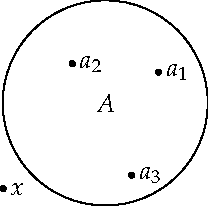
\includegraphics{sets-01-venn}
\end{defn}

As in the definition, it is typical to use upper-case letters ($A,B,C,\ldots$) for abstract sets and lower-case letters for their elements.\smallbreak

\emph{Venn diagrams} are useful for visualizing abstract sets. A set is represented by a region in the plane, with elements depicted by dots. The diagram in the definition represents a set $A$ comprising at least four elements $a_1,a_2,a_3$ and $x$. The element $y$ does not lie in $A$. 

\begin{example}{}{}
	Let $A$ be the set of (names of) US states. Then Michigan $\in A$ and Saskatchewan $\notin A$.
\end{example}

\begin{defn}{}{subset}
	Let $A$ and $B$ be sets.
	\begin{enumerate}
	  \item Sets are \emph{equal,} written $A=B$, if they have precisely the same elements.\par
	  \begin{minipage}[t]{0.74\linewidth}\vspace{-4pt}
	  	\item $A$ is a \emph{subset} of $B$, written $A\subseteq B$, if every element of $A$ is also an element of $B$.
	  	\item $A$ is a \emph{proper subset} of $B$ if $A\subseteq B$ and $A\neq B$. To stress this, we'd write $A\subsetneq B$. The Venn diagram on the right represents a proper subset. 
	  \end{minipage}
	  \hfill
	  \begin{minipage}[t]{0.25\linewidth}\vspace{-15pt}
			\flushright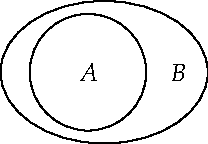
\includegraphics{sets-02-vennsubset}
	  \end{minipage}
	\end{enumerate}
\end{defn}

The following observations are simply translations of the definition:
\begin{enumerate}
  \item Equality: $A=B \iff A\subseteq B$ and $B\subseteq A$.
  \item Subset: $A\subseteq B \iff \bigl(x\in A\Longrightarrow x\in B\bigr) \iff \bigl(\forall x\in A, x\in B\bigr)$
  \item Not a subset: $A\nsubseteq B \iff \exists x\in A$ for which $x\notin B$.
\end{enumerate}


\boldsubsubsection{Roster \& Set-Builder Notation}

\emph{Roster notation} is the most basic way to describe the elements of a set: simply \emph{list} the elements in any order between curly brackets $\{\,,\,\}$.

\begin{example}{}{easysetnotation}
	Let $A$ be the set of (real number) solutions to the equation $2x^2-7x+3=0$ and let $B$ be the set of \emph{integer} solutions to the same equation. Since the polynomial factorizes as $(2x-1)(x-3)$, we see that $A=\{3,\frac 12\}$ and $B=\{3\}$. We could also write $A=\{\frac 12,3\}$ since \emph{order doesn't matter in roster notation.}	Moreover:
	\begin{itemize}
	  \item $A\nsubseteq B$ since $\frac 12\in A$ and $\frac 12\notin B$.
	  \item $B\subseteq A$ since 3 (the only element of $B$) lies in $A$. Indeed $B\subsetneq A$ is a  proper subset since $A\neq B$.
	\end{itemize}
\end{example}

Roster notation is ideal for small sets, but is of limited utility when trying to describe large sets. This is where our second notation rides to the rescue.\bigbreak

\emph{Set-builder notation} describes the elements of a set using some common property. Suppose $\cU$ is some (already understood) set and $P(x)$ is a propositional function with domain $\cU$, then
\[
	A:=\bigl\{x\in\cU:P(x)\bigr\} \tag{``$A$ is the set of $x$ in $\cU$ such that $P(x)$''}
\]
defines a set $A$ as \emph{the subset} of $\cU$ all of whose elements $x$ satisfy the property $P(x)$. A vertical separator $\mid$ is often used instead of a colon: we'll use both, though it might be essential in a given context to use one rather than the other for clarity.

\begin{examples}{}{}
\exstart Continuing Example \ref{ex:easysetnotation}, recall that $\R$ represents the set of real numbers and $\Z$ the set of integers. In set-builder notation, our solution sets may be written
	\[A=\bigl\{x\in\R:2x^2-7x+3=0\bigr\},\qquad B=\bigl\{x\in\Z:2x^2-7x+3=0\bigr\}\]
	In this case the qualifying proposition $P(x)$ is ``$2x^2-7x+3=0$.''
	\begin{enumerate}\setcounter{enumi}{1}
	  \item[]We can also express the fact that $B$ is a subset of $A$ in this notation (this time with a vertical separator),
	\[B=\bigl\{x\in A\bigm| x\in\Z\} \tag{``the set of elements $x$ in $A$ such that $x$ is an integer"}\]
	
	\item Let $X=\{2,4,6\}$ and $Y=\{1,2,5,6\}$. There are many options for how to write these in set-builder notation. For instance:
	\[
		X=\bigl\{n\in\Z:\tfrac 12n\in\{1,2,3\}\bigr\},\qquad Y=\bigl\{n\in\Z\bigm|1\le n\le 6\text{ and }n\neq 3,4\bigr\}
	\]
	We now practice the opposite skill by converting five sets from set-builder to roster notation.
	\begin{align*}
		&S_1=\bigl\{x\in X:x\text{ is divisible by 4}\bigr\}=\{4\}
		&&
		S_2=\bigl\{y\in Y:y\text{ is odd}\bigr\}=\{1,5\}
		\\
		&S_3=\bigl\{x\in X\bigm| x\in Y\bigr\}=\{2,6\}
		&&
		S_4=\bigl\{x\in X:x\notin Y\bigr\}=\{4\}
		\\
		&S_5=\bigl\{y\in Y\bigm| y\text{ is odd and $y-1\in X$}\}=\{5\}
	\end{align*}
	Can you find alternative descriptions in set-builder notation for the sets $S_1,\ldots,S_5$ above? Take your time getting used to this notation: the ability to translate between various descriptions of a set is \emph{crucial} to reading mathematics!
	
	\item We use the set $C=\{0,1,2,3,\ldots,24\}$ to describe $D=\{n\in\Z:n^2-3\in C\}$ in roster notation. Start by expanding the criterion for membership in $D$:
  \[
  	n^2-3\in C\iff n^2\in\bigl\{3,4,5,\ldots,25,26,27\bigr\}
  \]
  Since $n$ must be an integer, it follows that $D=\{\pm 2,\pm 3,\pm 4,\pm 5\}$.
  
  \item To express $E=\{0,2,6,12,\ldots\}$ in set-builder notation we might spot a pattern and decide that
  \[
  	E=\bigl\{n\in\Z: n=m(m+1) \text{ for some integer }m\ge 0\bigr\}
  \]
  The problem is that we cannot guarantee our correctness! Perhaps the correct formula is
  \[
  	n=m(m+1)+m(m-2)(m-6)(m-12)
  \]
	In the first case the next term in the sequence is $4\cdot 5=20$, whereas in the second case it is $20+128=148$. For larger sets, the clarity afforded by set-builder notation is essential!

	\end{enumerate}
\end{examples}



\boldsubsubsection{Common Sets of Numbers}

We've used some of this notation already, and much of the rest should be familiar.\vspace{-5pt}

\begin{quote}\def\arraystretch{1.15}
	\begin{tabular}{@{}ll}
		\emph{Natural numbers}&$\N=\bigl\{1,2,3,4,\ldots\bigr\}$ is the set of \emph{positive} integers.\\
		\emph{Integers}&$\Z=\bigl\{\ldots,-3,-2,-1,0,1,2,3,\ldots\bigr\}$.\\
		\emph{Rational numbers}&$\Q=\bigl\{\frac mn:m\in\Z\text{ and }n\in\N\bigr\} =\bigl\{\frac ab\bigm| a,b\in\Z\text{ and }b\neq 0\bigr\}$.\\
		\emph{Real numbers}&$\R$. Even a rudimentary definition is too involved for this text.\footnotemark\\
		\emph{Complex numbers}&$\C=\bigl\{x+iy:x,y\in\R\bigr\}$ where $i^2=-1$. We won't use these.
	\end{tabular}
\end{quote}

\vspace{-10pt}
	
\footnotetext{We simply assume the reader is comfortable with the idea of the real line where number corresponds to \emph{length.} A rigorous development of $\R$ is a matter for an upper-division \emph{analysis} course.}

\begin{examples}{}{}
	\exstart For instance: \ $7\in\N$, \ $\pi\in\R$, \ $-\frac 79\notin\Z$, \ $\sqrt 2\notin\Q$ \ and \ $3+\sqrt 5i\in\C$.
	\begin{enumerate}\setcounter{enumi}{1}%\itemsep2pt
	  \item The basic symbols can be decorated to make natural modifications. For example:
\vspace{-3pt}
		\begin{itemize}
		  \item $\N_0=\bigl\{0,1,2,3,4,\ldots\bigr\}=\Z^+_0=\bigl\{x\in\Z:x\ge 0\bigr\}$. Also called the \emph{whole numbers} ($\mathbb W$).
			\item $\Z_{\ge 5}=\bigl\{5,6,7,8,\ldots\bigr\} =\bigl\{x\in\Z:x\ge 5\bigr\}$ denotes the integers greater than or equal to 5.
		  \item $\R^+=\bigl\{x\in\R:x>0\bigr\}$ is the set of positive real numbers.
			\item $4\Z=\bigl\{\ldots,-8,-4,0,4,8,12,\ldots\bigr\} =\bigl\{x\in\Z: 4\mid x\bigr\}$ is the set\footnotemark{} of integer multiples of 4.\par
			This notation can be used for non-integer multiples, e.g. $\pi\Z=\bigl\{\ldots,-\pi,0,\pi,2\pi,\ldots\bigr\}$. 
			\item $2\Z+1=\bigl\{x\in\Z:x\equiv 1\pmod 2\bigr\}$ is the set of odd integers.
		\end{itemize}
		
		\item \emph{Intervals} are the most commonly encountered subsets of the real numbers. For instance:
% \vspace{-3pt}
		\begin{itemize}
		  \item $[1,\pi]=\bigl\{x\in\R\bigm|1\le x\le \pi\bigr\}$ is a \emph{closed} interval 
		  \item $[-4,7.21)=\{x\in\R\bigm|-4\le x<7.21\}$ is a \emph{half-open} interval.
		  \item $(-\infty, \sqrt 2) =\{x\in\R\bigm|x<\sqrt 2\}$ is an \emph{infinite (open)} interval.
		\end{itemize}
	\end{enumerate}
\end{examples}

\vspace{-5pt}

\footnotetext{Be careful!---the colon is the ``such that" separator while $\mid$ denotes the property ``4 divides $x$.''} %The unreadability of $\bigl\{x\in\Z\bigm| 4\mid x\bigr\}$ illustrates the benefit of having two separator symbols to choose from.}

\goodbreak

In view of the natural subset relationships $\N\subsetneq\Z\subsetneq\Q\subsetneq\R\subsetneq\C$, we consider a simple result.

\begin{lemm}{Transitivity of Subset}{subsettrans}
	Suppose $A\subseteq B$ and $B\subseteq C$. Then $A\subseteq C$.
\end{lemm}

\begin{proof}
	Think back to the criteria following Definition \ref{defn:subset}. Suppose $A\subseteq B$ and $B\subseteq C$. Then
	\[
		x\in A \overset{(A\subseteq B)}{\implies} x\in B\overset{(B\subseteq C)}{\implies} x\in C
	\]
	We conclude that $A\subseteq C$.
\end{proof}

Compare this to Exercise \ref*{sec:prop}.\ref{exs:iftransitive}: if we translate each subset relation into an implication, the proof structure is $(x\in A\Rightarrow x\in B)\wedge (x\in B\Rightarrow x\in C)\Longrightarrow (x\in A\Rightarrow x\in C)$. This is typical of basic results about sets: after translation, the theorem reduces to one of the standard rules of logic.



\boldsubsubsection{Cardinality and the Empty Set}

It is helpful to introduce some terminology to describe the \emph{size} of a set.

\begin{defn}{}{}
	A \emph{finite set} contains only a finite number of elements: this number is its \emph{cardinality,} written $\nm A$. A set with infinitely many elements is said to be an \emph{infinite set.}\par
	The symbol $\emptyset$ denotes the \emph{empty set}: a set containing no elements (cardinality zero: $\nm\emptyset=0$).
\end{defn}



\begin{examples}{}{}
	\exstart Let $A=\bigl\{1,3,\pi,\sqrt 2,103\bigr\}$, then $\nm A=5$.
	\begin{enumerate}\setcounter{enumi}{1}
		\item Let $B=\bigl\{4,\{1,2\},\{3\}\bigr\}$. The elements of $B$ are $4$, $\{1,2\}$ and $\{3\}$, therefore $\nm B=3$. It doesn't matter that the \emph{element} $\{1,2\}\in B$ is also a set!\par
		\begin{minipage}[t]{0.59\linewidth}\vspace{-5pt}
			\item Recall some basic trigonometry:
			\[
				\left\{x\in[0,4\pi]:\cos x=\frac 12\right\}=\left\{\frac{\pi}3,\frac{5\pi}3,\frac{7\pi}3,\frac{11\pi}3\right\}
			\]
			has cardinality 4.
		\end{minipage}
		\hfill
		\begin{minipage}[t]{0.4\linewidth}\vspace{-10pt}
			\flushright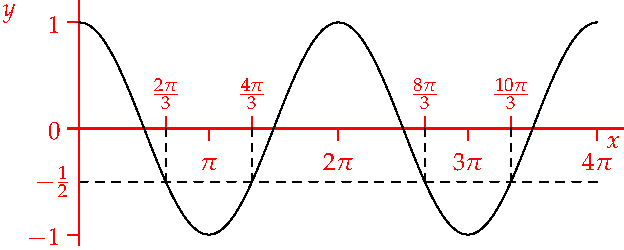
\includegraphics{sets-03-cos}
		\end{minipage}
		
		\item There are many representations of the empty set: for example
		\[
			\emptyset =\bigl\{x\in\R:x^2=-1\bigr\} = \bigl\{x\in\N:x^2+3x+2=0\bigr\}=\bigl\{n\in\N:n<0\bigr\}
		\]
		In general, if $X$ is any set and $P(x)$ is false for all $x\in X$, then\footnotemark{} $\emptyset=\bigl\{x\in X:P(x)\bigr\}$.
	\end{enumerate}
\end{examples}

\footnotetext{In some formalizations of set theory, the existence of the empty set is an axiom: an assumption made without proof. Provided one accepts that set-builder notation always defines a set---this is itself an axiom!---and that at least one set $X$ exists, the empty set may be \emph{defined} as in the example: a suitable property $P(x)$ might be something like ``$x\notin\{x\}$.''}


Cardinality is a very simple concept for finite sets; if $B$ is finite, so is any subset, and we have
\[
	A\subseteq B\implies \nm A\le \nm B
\]
For infinite sets, cardinality is more subtle. We'll return to this issue and uncover some of the bizarre and fun consequences of infinite cardinalities in Chapter \ref{chap:cantor}.
\bigbreak

We finish with a couple of simple results regarding the empty set.

\begin{lemm}{}{}
Let $A$ be a set.
\begin{enumerate}
  \item If $\nm A=0$, then $A=\emptyset$. The empty set is \emph{the unique set} with zero cardinality.
  \item $\emptyset\subseteq A$ and $A\subseteq A$
\end{enumerate}
\end{lemm}

\begin{proof}
	Think about the claim $\emptyset\subseteq A$: by the observations following Definition \ref{defn:subset}, this means
	\[
		x\in\emptyset\implies x\in A
	\]
	This is true (for any set $A$!) since there are no elements $x$ satisfying the hypothesis.\footnotemark{}
	\begin{enumerate}
 	 \item Suppose $A$ has cardinality zero. Repeating and combining with the above observation, we see that $\emptyset\subseteq A$ and $A\subseteq\emptyset$. We conclude that $A=\emptyset$.
 	 \item We already know that $\emptyset\subseteq A$. For the second part, simply observe that
 	 $x\in A\implies x\in A$.\qedhere
\end{enumerate}
\end{proof}

\footnotetext{If $P(x)$ is always false, then $(\forall x)\ P(x)\Longrightarrow Q(x)$ is true. This is called a \emph{vacuous} (empty) theorem.}

% 
% 
% \begin{examples}{}{}
% 	\begin{enumerate}\setcounter{enumi}{1}
%   \item Are the following sets equal?
%   \[E=\{n^2+2\in\Z:\text{$n$ is an odd integer}\},\qquad F=\{n\in\Z:n^2+2\text{ is an odd integer}\}.\]
%   It may help to first construct a table listing some of the values of $n^2+2$:
%   \[\begin{array}{c|c|c}
%   n&n^2&n^2+2\\\hline
%   \pm 1&1&3\\
%   \pm 3&9&11\\
%   \pm 5&25&27\\
%   \pm 7&49&51\\
%   \pm 9&81&83\\[-5pt]
%   \vdots&\vdots&\vdots
%   \end{array}\]
%   The set $E$ consists of those integers of the form $n^2+2$ where $n$ is an odd integer. By the table,
%   \[E=\{3,11,27,51,83,\ldots\}.\]
%   On the other hand, $F$ includes all those integers $n$ such that $n^2+2$ is odd. It is easy to see that
%   \[n^2+2\text{ is odd}\iff n^2\text{ is odd}\iff n\text{ is odd.}\]
%   Thus $F$ is simply the set of all odd integers:
%   \[F=\{\pm 1,\pm 3,\pm 5,\pm 7,\ldots\}=2\Z+1.\]
%   Plainly the two sets are not equal.
% 
%   \item $\{x\in\R:x^2-1=0\}\subseteq \{y\in\R:y^2\in\N\}$.\\
%   To make sense of this relationship, convert to roster notation: we obtain
%   \[\{-1,1\}\subseteq\{\pm\sqrt 1,\pm\sqrt 2,\pm\sqrt 3,\pm\sqrt 4,\ldots\}.\]
%   \item If $m$ and $n$ are positive integers, then $m\Z\subseteq n\Z\iff n\mid m$. Make sure you're comfortable with this! For example, $4\Z\subseteq 2\Z$ since every multiple of 4 is also a multiple of 2.
% \end{enumerate}
% \end{examples}


% \paragraph{Self-test Questions}
% 
% \begin{enumerate}
%   \item True or false: An open interval contains its endpoints.
%   \item True or false: $\{x\in\R:x^2<0\}$ is a representation of the empty set.
%   \item True or false: $\{x\in\Z:x\in[0,4)\}=\{0,1,2,3,4\}$.
% \end{enumerate}


\begin{exercises}{}{}
	A reading quiz and several questions with linked video solutions can be found \href{http://www.math.uci.edu/~ndonalds/math13/selftest/4-1-subset.html}{online}.


% Write the set $A=\{x\in\R:x^2+3x+2=0\}$ in roster notation.\\[5pt]
% 	We are looking for the set of all real number solutions to the quadratic equation $x^2+3x+2=0$. A simple factorization tells us that $x^2+3x+2=(x+1)(x+2)$, whence $A=\{-1,-2\}$.

	\begin{enumerate}
	  \item Describe the following sets in roster notation: that is, list their elements.
		\begin{enumerate}
		  \item \makebox[215pt][l]{$\bigl\{x\in\N:x^2\le 3x\bigr\}$\hfill (b)} \ $\bigl\{n\in\{0,1,2,3,\ldots,19\}:n+3\equiv 5\spmod 4\bigr\}$
		  \setcounter{enumii}{2}
		  \item \makebox[215pt][l]{$\bigl\{n\in\{-2,-1,0,1,\ldots,23\}:4\mid n^2\bigr\}$\hfill (d)} \ $\bigl\{x\in \frac 12\Z: 0\le x\le 4\text{ and }4x^2\in 2\Z+1\bigr\}$
		  \setcounter{enumii}{4}
		  \item $\bigl\{y\in\R:y=x^2\text{ for some $x\in\R$ with } x^2-3x+2=0\bigr\}$
		\end{enumerate}
			
			
		\item Describe the following sets in set-builder notation (\emph{look for a pattern}).
		\begin{enumerate}
		  \item \makebox[180pt][l]{$\bigl\{\ldots,-3,0,3,6,9,\ldots\bigr\}$\hfill (b)} \ $\bigl\{-3,1,5,9,13,\ldots\bigr\}$
		  \setcounter{enumii}{2}
		  \item $\bigl\{1,\frac 13,\frac 17,\frac 1{15},\frac 1{31},\ldots\bigr\}$
		\end{enumerate}
		  
	
	  \item Each of the following sets of real numbers is a single interval. Determine the interval.
		\begin{enumerate}
		  \item \makebox[180pt][l]{$\bigl\{x\in\R:x>3\text{ and }x\le 17\bigr\}$\hfill (b)} \ $\bigl\{x\in\R:x\nleq 3\text{ or }x\le 17\bigr\}$
		  \setcounter{enumii}{2}
		  \item \makebox[180pt][l]{$\bigl\{x^2\in\R:x\neq 0\bigr\}$ \hfill (d)} \ $\bigl\{x\in\R^-:x^2\ge 16\text{ and }x^3\le 27\bigr\}$
		\end{enumerate}
			
			
		\item Is the set $\{x\in\Z:-1\le x<43\}$ finite or infinite? If finite, what is its cardinality?
				
		
		%\item Compare the sets $A=\{3x\in\Z:x\in 2\Z\}$ and $B=\{x\in\Z:x\equiv 12\pmod 6\}$. Are they equal?
			
			
		\item What is the cardinality of the set $\Bigl\{\emptyset,\bigl\{\emptyset\bigr\},\bigl\{\emptyset,\{\emptyset\}\bigr\}\Bigr\}$? \ What are its elements?
		
		\item Let $A=\emptyset$, \ $B=\{A\}$, \ $C=\bigl\{\{A\}\bigr\}$ \ and \ $D=\bigl\{A,\{0\},\{0,1\}\bigr\}$.\par
	  Answer the following true or false:
	  \begin{enumerate}
	    \item \makebox[80pt][l]{$0\in A$\hfill (b)} \ \makebox[80pt][l]{$A\in B$\hfill (c)} \ \makebox[80pt][l]{$A\in C$\hfill (d)} \ \makebox[80pt][l]{$B\in C$ \hfill (e)} \ $A\in D$
	    \setcounter{enumii}{5}
	    \item \makebox[80pt][l]{$B\in D$\hfill (g)} \ \makebox[80pt][l]{$0\in D$\hfill (h)} \ \makebox[80pt][l]{$\{0\}\in D$\hfill (i)} \ $\{1\}\in D$
	  \end{enumerate}
	  
	  
	  \item List all the \emph{proper} subsets of $\{1,2,3\}$.
	  
	    
		\goodbreak
	   
		   
		\item Let $A,B,C,D$ be the following sets:
	  \begin{align*}
	  	&A=\{-4,1,2,4,10\}
	  	&&B=\bigl\{m\in\Z:\nm m\le 12\bigr\}\quad \text{(\emph{absolute value of $m$})}\\
	  	&C=\bigl\{n\in\Z:n^2\equiv 1\spmod 3\bigr\}
	  	&&D=\bigl\{t\in\Z:t^2+3\in [4,20)\bigr\}  
	  \end{align*}
	  Of the 12 subset relations $A\subseteq B$,\ $A\subseteq C,\ldots, D\subseteq C$, which are true and which false?
	  
	  \item Let $A=\bigl\{1,2,\{1,2\},\{3\}\bigr\}$ and $B=\{1,2\}$. Answer the following true or false:
	  \begin{enumerate}
	    \item \makebox[100pt][l]{$B\in A$\hfill (b)} \ \makebox[100pt][l]{$B\subseteq A$\hfill (c)} \ \makebox[100pt][l]{$3\in A$\hfill (d)} \ $\{3\}\subseteq A$
	    \setcounter{enumii}{4}
	    \item \makebox[100pt][l]{$\{3\}\in A$\hfill (f)} \ \makebox[100pt][l]{$\emptyset\subseteq A$\hfill (g)} \ $\emptyset\in A$
	  \end{enumerate}
	  
	  \item Let $A=\{0,2,4,6,8,10\}$. Write the set $B=\{X\subseteq A:|X|=2\}$ in roster notation.
	  
	    
	  \item\begin{enumerate}
	    \item Suppose $A\subseteq B\subseteq C\subseteq A$. Show that $A=B=C$.
	    \item Is it possible for sets $A,B,C$ to satisfy $A\subsetneq B\subseteq C\subseteq A$? Why/why not?
	  \end{enumerate}

	
		\item Let $A=\{\text{1,2,3,4}\}$, and let $B =\bigl\{\{x,y\}:x,y\in A\bigr\}$.
		\begin{enumerate}
	  	\item Describe $B$ in roster notation (\emph{what happens when $x=y$?}).
			\item Find the cardinalities of the following sets:
			\[
				C=\Bigl\{\bigl\{x,\{y\}\bigr\}:x,y\in A\Bigr\}
				\quad\text{and}\quad
				D=\biggl\{\Bigl\{\bigl\{x,\{y\}\bigr\}:x,y\in A\Bigr\}\biggr\}
			\]
		\end{enumerate}
  
  
  	\item Let $A=\{x\in\R:x^3+x^2-x-1=0\}$ and $B=\{x\in\R:x^4-5x^2+4=0\}$. Are either of the relations $A\subseteq B$ or $B\subseteq A$ true? Explain.
  
  
  	\item For which real numbers $x>0$ do we have $[0,x]\subsetneq[0,x^2]$? Prove your assertion.
  
  
  	\item Let $m,n\in\N$. Prove: $m\Z\subseteq n\Z\iff n\mid n$.

  
  	\item\label{ex:mirrored} Given $A\subseteq\Z$ and $x\in\Z$, we say that $x$ is $A$-mirrored if and only if $-x\in A$. Also define
  	\[
			M_A:=\bigl\{x\in\Z: x\text{ is $A$-mirrored}\bigr\}
		\]
		\begin{enumerate}
	  	\item What does it mean for $x$ \emph{not} to be $A$-mirrored?
	  	\item Find $M_B$ given $B=\{0,1,-6,-7,7,100\}$.
	  	\item Assume that $A \subseteq\Z$ is closed under addition: for all $x,y\in A$, we have $x+y\in A$. Show that $M_A$ is closed under addition.
	  	\item In your own words, under which conditions is $A=M_A$?
		\end{enumerate}

  \item Define the set $[1]=\bigl\{x\in\Z: x\equiv 1\spmod 5\bigr\}$.
		\begin{enumerate}
		  \item Describe the set $[1]$ in roster notation.
		  \item Compute the set $M_{[1]}$, as defined in Exercise \ref{ex:mirrored}. Is $M_{[1]}$ equal to $[1]$?
			\item Now consider the set $[10]=\{x\in\Z:x\equiv 10\spmod 5\}$. Are the sets $[10]$ and $M_{[10]}$ equal? Prove or disprove.
  	\end{enumerate}


     % \item (Hammack's \href{http://www.people.vcu.edu/~rhammack/BookOfProof/}{\emph{Book of Proof}}, Section 1.3, Exercise 6)
%List all subsets of $\{\R,\Q,\N\}$.
    

		\item Consider the set $A=\{a,b,c,d\}$. 
    \begin{enumerate}
      \item Of each cardinality 0, 1, 2, 3 and 4, how many subsets has $A$? Is there a pattern?
        
      \item Completely expand the polynomial $(1 + x)^4$. What do you notice about the coefficients? 
    \end{enumerate}

	\end{enumerate}
\end{exercises}

\clearpage



\subsection{Unions, Intersections and Complements}\label{sec:union}

In this section we construct new sets from old, modeled precisely on the logical concepts of \emph{and, or,} and \emph{not} (compare Definition \ref{defn:andornot}). 


\begin{defn}{}{unionint}
	Let $\cU$ be a (universal) set,\footnotemark{} and suppose $A,B$ are subsets of $\cU$.
	\begin{enumerate}\itemsep0pt
		\item The \emph{union} of $A$ and $B$ is the set of elements in $A$ or $B$:
		\[
			\makebox[210pt][l]{$A\cup B:=\bigl\{x\in\cU:x\in A\text{ or }x\in B\bigr\}$\hfill} (x\in A\cup B\iff x\in A\text{ or }x\in B)
		\]
		\item The \emph{intersection} of $A$ and $B$ is the set of elements in both $A$ and $B$:
		\[
			\makebox[210pt][l]{$A\cap B:=\bigl\{x\in\cU:x\in A\text{ and }x\in B\bigr\}$\hfill} (x\in A\cap B\iff x\in A\text{ and }x\in B)
		\]
		We say that $A$ and $B$ are \emph{disjoint} if $A\cap B=\emptyset$.
	  \item The \emph{complement} of $A$ is the set of all elements not in $A$:
		\[
			\makebox[210pt][l]{$\comp A:=\bigl\{x\in\cU:x\notin A\bigr\}$ \hfill} (x\in\comp A\iff x\notin A \ (\text{and }x\in\cU))
		\]
		This can be read ``$B$ minus $A$'', indeed some authors write $B-A$. Similarly $\comp A=\cU\setminus A$, etc.
		\item The \emph{complement of $A$ relative $B$} is the set of elements in $B$ which are not in $A$:
		\[
			\makebox[210pt][l]{$B\setminus A:=B\cap \comp A=\bigl\{x\in B:x\notin A\bigr\}$\hfill} (x\in B\setminus A\iff x\in B\text{ and } x\notin A)
		\]
	\end{enumerate}
	
	\begin{center}
		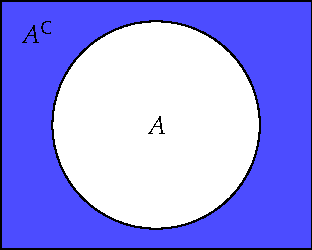
\includegraphics{sets-05-venncomp}
		\qquad\qquad
		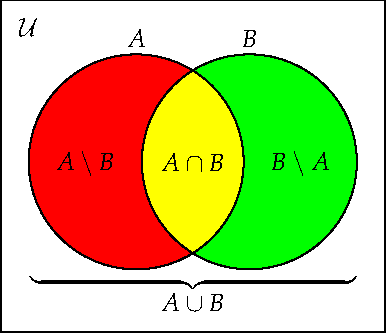
\includegraphics{sets-04-vennunion}
	\end{center}
\end{defn}

\footnotetext{Of which everything else will be a subset. This is needed particularly for complements, but more generally is required to invoke set-builder notation. In certain contexts, the universal set is naturally assumed: $\cU=\R$ makes sense if you are working within the real numbers, $\cU=\Z$ if doing modular arithmetic.}

In the Venn diagrams, the outer box depicts the universal set $\cU$. Though it doesn't constitute a proof, the diagram makes certainly suggests that
\[
	A=(A\setminus B)\cup (A\cap B) \quad\text{and}\quad B=(B\setminus A)\cup(A\cap B)
\]
Observe the notational similarity with logic: $\cup$ looks a bit like $\vee$ (OR); $\cap$ like $\wedge$ (AND).

\begin{examples}{}{}
	\exstart Let $\cU=\{1,2,3,4,5\}$, $A=\{1,2,3\}$, and $B=\{2,3,4\}$. Then
	\begin{align*}
		&\comp A=\{4,5\} &&\comp B=\{1,5\} &&B\setminus A=\{4\} &&A\setminus B=\{1\}\\
		&A\cup B=\{1,2,3,4\} &&A\cap B=\{2,3\} &&A\cap\comp B=\{1\} &&\comp A\cup\comp B=\{1,4,5\}
	\end{align*}
	
	\goodbreak
		
	\begin{enumerate}\setcounter{enumi}{1}
		\item Using interval notation, let $\cU=[-4,5]$, \ $A=[-3,2]$, \ and \ $B=[-4,1)$. Then\par
% 		\begin{align*}
% 			&\comp A=[-4,-3)\cup (2,5] &&\comp B=[1,5] &&A\cup B=[-4,2] \\
% 			&A\setminus B=[1,2] &&B\setminus A=[-4,-3) &&A\cap B=[-3,1) 
% 		\end{align*}
% 		\vspace{-24pt}
% 		\begin{center}
% 		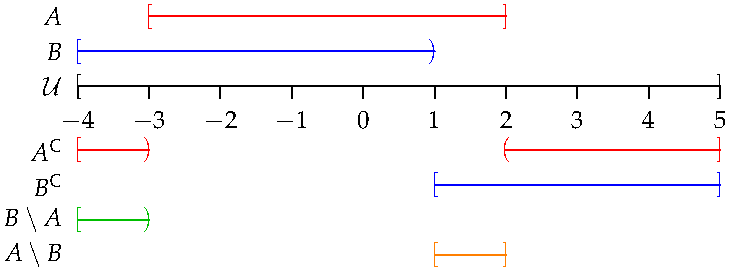
\includegraphics[width=0.7\textwidth]{sets-13-intervalex}
% 		\end{center}
% 		\vspace{-13pt}
		\begin{minipage}[t]{0.3\linewidth}\vspace{-13pt}
			\begin{gather*}
			\comp A=[-4,-3)\cup (2,5]\\
			\comp B=[1,5]\\
			A\setminus B=[1,2]\\
			B\setminus A=[-4,-3)\\
			A\cup B=[-4,2]\\
			A\cap B=[-3,1) 
			\end{gather*}
		\end{minipage}
		\hfill
		\begin{minipage}[t]{0.69\linewidth}\vspace{0pt}
			\flushright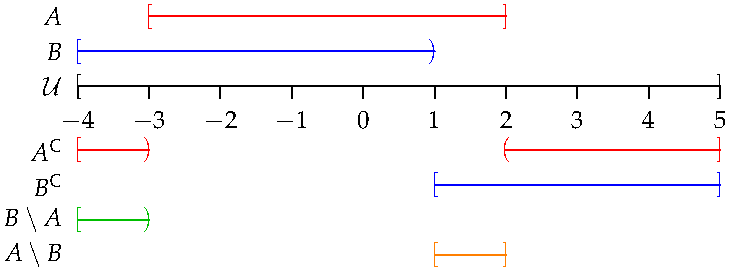
\includegraphics[scale=0.8]{sets-13-intervalex}
		\end{minipage}
		\smallbreak
		While you should be comfortable with these just from the picture, for practice it is worth trying algebraic arguments. In particular, note how $\comp A$ relies on de Morgan's law (Theorem \ref{thm:demorgan}):
		\begin{align*}
			x\in \comp A&\iff x\notin A\iff \neg\bigl(x\in A\bigr) \iff\neg\bigl(-3\le x \text{ and }x\le 2\bigr)\\
			&\iff x<-3\text{ or }x>2 \tag{de Morgan}\\
			&\iff x\in[-4,-3)\cup (2,5] \tag{remember that $x\in\cU$ always!}
		\end{align*}
		
		\item Let $A=(-\infty,3)$ and $B=[-2,\infty)$ in interval notation. Then $A\cup B=\R$ and $A\cap B=[-2,3)$.
	\end{enumerate}
\end{examples}


For the remainder of this section, we summarize the basic rules of set algebra.

\begin{thm}{Union/intersection rules}{setbasic}
	Let $A,B,C$ be sets. Then:
	\begin{enumerate}\itemsep2pt
		\item $\emptyset\cup A=A$ \ and \ $\emptyset\cap A=\emptyset$
		\item $A\cap B\subseteq A\subseteq A\cup B$
		\item $A\cup B=B\cup A$ \ and \ $A\cap B=B\cap A$
		\item $A\cup (B\cup C)=(A\cup B)\cup C$ \ and \ $A\cap (B\cap C)=(A\cap B)\cap C$
		\item $A\cup A=A\cap A=A$
		\item $A\subseteq B\Longrightarrow A\cup C\subseteq B\cup C$ \ and \ $A\cap C\subseteq B\cap C$
	\end{enumerate}
\end{thm}

If you don't believe a result, try \emph{visualizing} it using a Venn diagram. The basic proof strategy is the same for all parts: convert each statement into propositions (Definition \ref{defn:unionint} parentheses) and use what you know from basic logic (e.g., Theorem \ref{thm:demorgan} and page \pageref{pg:asidelogicalgebra}). We prove part 2 and half of part 6, leaving some of the rest to the Exercises.

\begin{proof}
\begin{enumerate}
  \item[2.] There are two results here: $A\cap B\subseteq A$ and $A\subseteq A\cup B$. We prove separately, with some commentary on the side.
	\begin{enumeratea}
		\item Suppose $x\in A\cap B$.\hfill(Goal: want to prove $x\in A\cap B\Rightarrow x\in A$)\par
		Then $x\in A$ and $x\in B$.\hfill(Definition of intersection)\par
		Plainly $x\in A$. We conclude that $A\cap B\subseteq A$\hfill(Definition of subset)
		\item Suppose $y\in A$.\hfill(Goal: prove $y\in A\Rightarrow y\in A\cup B$)\par
		Then ``$y\in A$ or $y\in B$'' is true, whence $y\in A\cup B$.\hfill(Definition of union/or)\par
	  We conclude that $A\subseteq A\cup B$.
	\end{enumeratea}
	
	\goodbreak
	
	\item[6.] (first half)\lstsp Suppose $A\subseteq B$. We wish to prove that $x\in A\cup B\Longrightarrow x\in A\cup C$. However,
	\begin{align*}
		x\in A\cup C&\implies x\in A\text{ or }x\in C\tag{definition of union}\\
		&\implies x\in B\text{ or }x\in C\tag{since $A\subseteq B$}\\
		&\implies x\in B\cup C \tag*{\qedhere}
	\end{align*}
\end{enumerate}
\end{proof}



The next batch of rules describe how complements interact with other set operations: parts 1 and 2 are \emph{de Morgan's laws for sets}; unsurprisingly, their proofs depend on the corresponding laws of logic.


\begin{thm}[lower separated=false, sidebyside, sidebyside align=top seam, sidebyside gap=0pt, righthand width=0.4\linewidth]{Complement rules}{setcomp}
	Let $A,B$ be sets. Then:
	\begin{enumerate}\itemsep2pt
		\item $\comp{(A\cap B)}=\textcolor{blue}{\comp A}\cup \textcolor{red}{\comp B}$ (see picture)
		\item $\comp{(A\cup B)}=\comp A\cap \comp B$
		\item $\smash[t]{\comp{(\comp A)}}=A$
		%\item $A\setminus B=A\cap\comp B$
		\item $A\subseteq B\iff \comp B\subseteq \comp A$
	\end{enumerate}
	\tcblower
	\flushright
	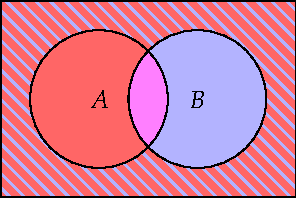
\includegraphics[scale=1]{sets-08-venndemorgan2}
\end{thm}

% \begin{proof}[Proof of 1.]
% We start by trying to show that the left hand side is a subset of the right hand side.
% \begin{align*}
% x\in\comp{(A\cap B)}&\implies x\notin A\cap B\\
% &\implies x\text{ is not a member of \emph{both} $A$ and $B$}\\
% &\implies x\text{ is not in \emph{at least one} of $A$ and $B$}\\
% &\implies x\notin A\text{ or }x\notin B\\
% &\implies x\in\comp A\text{ or }x\in\comp B\\
% &\implies x\in\comp A\cup\comp B
% \end{align*}
% With a little thinking, we realize that all of the $\Longrightarrow$ arrows may be replaced with if and only if arrows $\Longleftrightarrow$ without compromising the argument. We've therefore shown that the sets $\comp{(A\cap B)}$ and $\comp A\cup \comp B$ have the same elements, and are thus equal.
% \end{proof}


\begin{proof}
	We prove only part 1. As before, the natural approach is to restate the result using propositions.
	\begin{align*}
		x\in\comp{(A\cap B)}&\iff \neg\bigl(x\in A\cap B\bigr) \iff \neg\bigl(x\in A\ \text{ and }\  x\in B\bigr)\\
		&\iff \neg\bigl(x\in A\bigr)\ \text{ or }\ \neg\bigl(x\in B\bigr) \tag*{(de Morgan's first law of logic)}\\
		&\iff x\in\comp A\ \text{ or }\ x\in\comp B\\
		&\iff x\in\comp A\cup\comp B\tag*{\qedhere}
	\end{align*}
\end{proof}

Our final pair of results describe the interaction of unions and intersections.\par

\begin{thm}[lower separated=false, sidebyside, sidebyside align=top seam, sidebyside gap=0pt, righthand width=0.3\linewidth]{Distributive laws}{setdist}
	For any sets $A,B,C$:
	\begin{enumerate}\setlength{\itemsep}{2pt}
		\item $A\cap(B\cup C)=(A\cap B)\cup(A\cap C)$
		\item $A\cup(B\cap C)=(A\cup B)\cap(A\cup C)$
	\end{enumerate}
	The Venn diagram illustrates the second result: think about adding the colored regions.
	\tcblower
	\flushright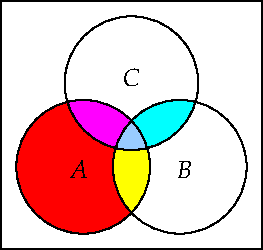
\includegraphics{sets-07-venndist}
\end{thm}


% 
% \begin{proof}
% \begin{itemize}
%   \item[($\subseteq$)] Let $x\in A\cup (B\cap C)$. Then $x\in A$ or $x\in B\cap C$. There are two cases:
%   \begin{itemize}
%     \item[(a)] If $x\in A$, then $x\in A\cup B$ and $x\in A\cup C$ by Theorem \ref{thm:setbasic}, part 2.
%     \item[(b)] If $x\in B\cap C$, then $x\in B$ and $x\in C$. It follows that $x\in A\cup B$ and $x\in A\cup C$, again by Theorem \ref{thm:setbasic}.
%   \end{itemize}
%   In both cases $x\in (A\cup B)\cap(A\cup C)$.
%   \item[($\supseteq$)] Let $y\in (A\cup B)\cap(A\cup C)$. Then $y\in A\cup B$ and $y\in A\cup C$. There are again two cases:
%   \begin{itemize}
%     \item[(a)] If $y\in A$, then we are done, for then $y\in A\cup (B\cap C)$.
%     \item[(b)] If $y\notin A$, then $y\in B$ and $y\in C$. Hence $y\in B\cap C$. In particular $y\in A\cup (B\cap C)$.
%   \end{itemize}
%   In both cases $y\in A\cup (B\cap C)$.\qedhere
% \end{itemize}
% \end{proof}


\begin{proof}
	We prove only the first result.
	\begin{align*}
		x\in A\cap(B\cup C) &\iff x\in A\text{ and }x\in B\cup C\\
		&\iff x\in A \text{ and }\bigl(x\in B\text{ or }x\in C\bigr)\\
		&\iff \bigl(x\in A \text{ and }x\in B\bigr)\text{ or }\bigl(x\in A\text{ and }x\in C\bigr) \tag{distributive law, page \pageref{pg:asidelogicalgebra}}\\
		&\iff x\in A\cap B\text{ or }x\in A\cap C\\
		&\iff x\in (A\cap B)\cup(A\cap C)\tag*{\qedhere}
	\end{align*}
\end{proof}

\goodbreak

% \paragraph{Self-test Questions}
% 
% \begin{enumerate}
%   \item The set operations of complement, union and intersection are based, respectively, on the logical constructions \underline{\phantom{not\quad}}, \underline{\phantom{or\quad}}, and \underline{\phantom{and\quad}}.
%   \item The result $\comp{(A\cup B)}=\comp A\cap\comp B$ is one of \underline{\phantom{De Morgan's laws\qquad}}.
%   \item True or false: if $A$ and $B$ are finite sets, then $A\cap B$ has strictly smaller cardinality than $A$.
%   \item True or false: if $A$ is a finite set, then $\comp A$ is a finite set.
%   \item True of false: if $A$ and $B$ are finite sets, then $\nm{A\cup B}\le\max(\nm A,\nm B)$.
% \end{enumerate}

\begin{exercises}{}{}
	A reading quiz and several questions with linked video solutions can be found \href{http://www.math.uci.edu/~ndonalds/math13/selftest/4-2-union.html}{online}.
	
	\begin{enumerate}
	  \item Describe each set simply as you can: e.g., 
	  \[
	  	\bigl\{x\in\R:x^2<9\text{ and } x^3<8\bigr\}= (-3,3)\cap(-\infty,2) =(-3,2)
	  \]
	  \begin{enumerate}
		 	\item $\bigl\{x\in\R:x^2\neq x\bigr\}$
			\item $\bigl\{x\in\R:x^3-2x^2-3x\le 0\text{ or }x^2=4\bigl\}$
			\item $\bigl\{y\in\R:\exists x\in\R \text{ with }y=x^2 \text{ and }x\neq 1\bigl\}$
			\item $\bigl\{z\in\Z:z^2\text{ is even and $z^3$ is odd}\bigl\}$
			\item $\bigl\{y\in 3\Z+2:y^2\equiv 1\spmod 3\bigl\}$
		\end{enumerate}
	  
	  \item Let $A=\{1,3,5,7,9\}$, $B=\{1,4,7,10\}$ and $\cU=\{1,2,\ldots,10\}$. What are the following sets?
	    \begin{enumerate}
		  	\item \makebox[100pt][l]{$A\cap B$\hfill (b)} \ \makebox[100pt][l]{$A\cup B$\hfill (c)} \ \makebox[100pt][l]{$B\setminus A$\hfill (d)} \ $\comp A$ 
		  	\setcounter{enumii}{4}
		  	\item \makebox[100pt][l]{$\comp{(A\setminus B)}$ \hfill (f)} \ \makebox[100pt][l]{$\comp A\cap \comp B$\hfill (g)} \ $(A\cup B)\setminus (A\cap B)$
			\end{enumerate}
	
  	
% 	\item Consider Theorems \ref{thm:setbasic} and \ref{thm:setdist}. In all seven results, replace the symbols in the first row of the following table with those in the second. Which of the results seem familar? Which are false?
% \[\begin{array}{c|c|c|c|c}
% \emptyset&A,B,C\text{ sets}&\cup&\cap&\subseteq\\\hline
% 0&A,B,C\in\N_0&+&\cdot&\le
% \end{array}\]

	%\item Prove that $B\setminus A=B\iff A\cap B=\emptyset$.
	
		\item Give formal proofs of the following parts of Theorems \ref{thm:setbasic}, \ref{thm:setcomp} and \ref{thm:setdist}. %With practice you should be able to prove \emph{all} of parts of these theorems \emph{without} looking at the arguments in the notes!
		\begin{enumerate}
		  \item \makebox[180pt][l]{$\emptyset\cap A=\emptyset$\hfill (b)} \ $A\cap (B\cap C)=(A\cap B)\cap C$
		  \setcounter{enumii}{2}
			\item \makebox[180pt][l]{$\comp{(\comp A)}=A$\hfill (d)} \ $A\cup(B\cap C)=(A\cup B)\cap(A\cup C)$
			\setcounter{enumii}{4}
			\item $A\subseteq B\iff \comp B\subseteq \comp A$
		\end{enumerate}
	
	
		\item By showing that each side is a subset of the other, give a formal proof of the set identity
		\[
			A=(A\setminus B)\cup (A\cap B)
		\]
		Now repeat your argument using only results from set algebra (Theorems \ref{thm:setcomp} and \ref{thm:setdist}).
	
	
	\item Prove the identity $A\cup B=A\iff B\subseteq A$ for any sets $A,B$.
	
	
	\item Prove the identities for any sets $A,B,C$:
	\begin{enumerate}
	  \item $\comp{(A\cap B\cap C)}=\comp A\cup\comp B\cup\comp C$
	  \item $(A\cup B)\setminus (A\cap B)=(A\setminus B)\cup (B\setminus A)$
	\end{enumerate}
	
		
	\item Prove or disprove the following conjectures (\emph{Hint: revisit Section \ref{sec:proof2}}).
	 \begin{enumerate}
	    \item $\exists x\in\R\setminus\Q$ such that $x^2\in\Q$. \qquad\qquad (b) \ $\forall x\in\R\setminus\Q$ we have $x^2\in\Q$.
		\end{enumerate}
	
	
	  \item Let $A\subseteq\R$, and let $x\in\R$. We say that $x$ is \emph{far away} from the set $A$ if and only if:
	  \[
	  	\exists d>0 \ \text{ such that } A\cap[x-d,x]=\emptyset
	  \] 
		If this does not happen, we say that $x$ is \emph{close to} $A$.
  	\begin{enumerate}
			\item Draw a picture of a set $A$ and elements $x,y$ such that $x$ is \emph{far away} from and $y$ is \emph{close to} $A$. 
			\item State the meaning of ``$x$ is close to $A$'' \ (negate ``$x$ is far away from $A$'').
			%\item Let $A=\{1,2,3\}$. Show that $x=4$ is \emph{far away} from $A$ using the definition.
			%\item Let $A=\{1,2,3\}$. Show that $x=1$ is \emph{close} to $A$.
			\item Let $A=\{1,2,3\}$.
			\begin{enumerate}
			  \item Show that $x=4$ is \emph{far away} from $A$ using the definition.
				\item Let $A=\{1,2,3\}$. Show that $x=1$ is \emph{close} to $A$.
			\end{enumerate}
			\item For general $A\subseteq\R$, show that if $x\in A$, then $x$ is \emph{close} to $A$.
			\item Let $A=(a,b)$ be a bounded interval. Is the end-point $a$ \emph{far away} from $A$?  What about $b$?
  	\end{enumerate}
  	
	\end{enumerate}

\end{exercises}

\clearpage



\subsection{Introduction to Functions}\label{sec:func1}

Sets become a lot more useful and interesting once you start transforming their elements! This is accomplished using \emph{functions.} In this section we introduce some basic concepts and notation, much of which should be familiar. A formal definition will be given in Chapter \ref{chap:relations}, but for the present the following will suffice.

\begin{defn}{}{function1}
	Let $A,B$ be sets. A \emph{function} $f:A\to B$ is a rule assigning to each input $a\in A$ a single output $b\in B$, typically denoted $f(a)$.	Various sets are associated to $f$:\par
	\begin{minipage}[t]{0.61\linewidth}\vspace{-5pt}
	\emph{Domain}: $\dom(f)=A$ is the set of inputs to the function.\smallbreak
	\emph{Codomain}: $\operatorname{codom}(f)=B$ is the set of potential outputs.\smallbreak
	\emph{Image} of a subset $U\subseteq A$: the set of outputs given inputs in $U$
	\[
		f(U):=\bigl\{f(u)\in B:u\in U\bigr\}
	\]
	\emph{Range}: $\range(f)=f(A)=\{f(a)\in B:a\in A\}$ is the set of realized outputs.
		\end{minipage}
		\hfill
		\begin{minipage}[t]{0.38\linewidth}\vspace{-3pt}
			\flushright
   		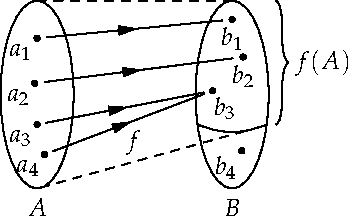
\includegraphics[scale=1]{sets-16-funcdef2}
		\end{minipage}\medbreak
	\emph{Inverse image} (or \emph{pre-image}) of a subset $V\subseteq B$: the set of inputs which are mapped into $V$
	\[
		f^{-1}(V):=\bigl\{a\in A:f(a)\in V\bigr\}
	\]
\end{defn}

The rule defining a function can be described using arrow notation $f:a\mapsto b$.

\begin{examples}{}{functions}
	\exstart Functions whose codomain is (a subset of) the real numbers $\R$ are often \textcolor{blue}{graphed}: the \textcolor{Purple}{domain} and \textcolor{Green}{range} are found by projecting the graph onto the two axes.\par
	\begin{enumerate}\setcounter{enumi}{1}
		\begin{minipage}[t]{0.6\linewidth}\vspace{-8pt}
			\item[]For instance if $f:[-3,2)\to\R$ is the square function
			\[
				f:x\mapsto x^2 \tag{equivalently $f(x)=x^2$}
			\]
			then $\textcolor{Purple}{\dom(f)=[-3,2)}$ and $\textcolor{Green}{\range(f)=[0,9]}$. We could also calculate other images/pre-images, for example,
  		\begin{gather*}
  			f\bigl([-1,2)\bigr)=\bigl\{x^2:-1\le x<2\bigr\}=[0,4)\\[3pt]
  			\begin{aligned}
  				f^{-1}\bigl((-10,2]\bigr)&=\bigl\{x\in[-3,2):-10<x^2\le 2\bigr\}\\
  				&=[-\sqrt 2,\sqrt 2]
  			\end{aligned}
  		\end{gather*}
		\end{minipage}
		\hfill
		\begin{minipage}[t]{0.39\linewidth}\vspace{-8pt}
			\flushright
  		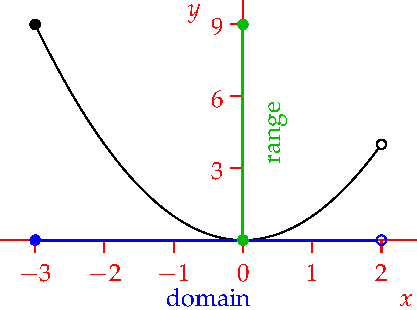
\includegraphics{sets-10-rangedom}
		\end{minipage}
		
 	  \bigbreak
		

	\begin{minipage}[t]{0.64\linewidth}\vspace{0pt}
		\item Define $f:\Z\to\{0,1,2\}$ by $f:n\mapsto n^2\pmod 3$. The table shows a few examples (remember $\dom(f)=\Z$ is infinite!).
	\end{minipage}
	\hfill
	\begin{minipage}[t]{0.35\linewidth}\vspace{0pt}
		\flushright
		$\begin{array}{c|cccccccc}
  		n&0&1&2&3&4&5&6&7\\\hline
  		f(n)&0&1&1&0&1&1&0&1
  	\end{array}$
	\end{minipage}\par
		Exercise \ref*{sec:cong}.\ref{exs:nsquaredrem} confirms what the examples suggest, that $\range(f)=\{0,1\}$. We also compute a single inverse image (revisit the previous two sections if you're unsure about the notation):
		\begin{align*}
			f^{-1}\bigl(\{1\}\bigr) &=\bigl\{x\in\Z:x^2\equiv 1\spmod 3\bigr\} =\bigl\{x\in\Z:x\equiv 1\text{ or }2\spmod 3\bigr\}\\
			&=(3\Z+1)\cup(3\Z+2)
		\end{align*}

  \begin{minipage}[t]{0.64\linewidth}\vspace{0pt}
    \item\label{ex:functmod} Let $A=\{0,1,2,\ldots,7\}$ be the set of remainders modulo 8 and define two functions $f,g:A\to A$:
    \[
    	f(n)=3n\spmod{8}\qquad g(n)=6n\spmod 8
    \]
  \end{minipage}
  \hfill
  \begin{minipage}[t]{0.35\linewidth}\vspace{0pt}
  	\flushright
  	$\begin{array}{c|cccccccccc}
  		n&0&1&2&3&4&5&6&7\\\hline
  		f(n)&0&3&6&1&4&7&2&5\\\hline
  		g(n)&0&6&4&2&0&6&4&2
  	\end{array}$	
  \end{minipage}
  \smallbreak
  Since the domain has only 8 elements, the table describes everything. Observe that
  \begin{align*}
  	&\range(f)=A &&f\bigl(\{1,5\}\bigr) =\{3,7\} &&f^{-1}\bigl(\{1,2,3,4\}\bigr) =\{1,3,4,6\}\\
  	&\range(g)=\{0,2,4,6\} &&g\bigl(\{1,5\}\bigr) =\{6\} &&g^{-1}\bigl(\{1,2,3,4\}\bigr) =\{2,3,5,7\}
  \end{align*}
  	
  \item Let $A=\{0,1,2,3,4\}$ and let $B=\{$two-element subsets of $A\}$. Define
  \[
  	f:A\to B:a\mapsto \{a,a+1\negthickspace \spmod 5\}
  \]
  where we take the remainder modulo 5. You should be able to convince yourself that
  \begin{gather*}
  	\range(f)=\big\{ \{0,1\}, \{1,2\}, \{2,3\}, \{3,4\}, \{4,0\} \big\}\\[3pt]
  	f\bigl(\{1,4\}\bigr)=\big\{f(1),f(4)\big\}=\big\{\{1,2\},\{4,0\}\big\} \quad\text{and}\quad f^{-1}\bigl\{\{2,4\},\{4,0\}\bigr\}=\{4\}
  \end{gather*}
	\end{enumerate}
  
\end{examples}


\boldsubsubsection{Injections, Surjections and Invertibility}

We turn our attention to perhaps the most important properties a function can possess.

\begin{defn}{}{11}
	Let $f:A\to B$ be a function. We say that $f$ is:
	\begin{enumerate}
	  \item \emph{Injective} (\emph{1--1}, an \emph{injection}) if it never outputs the same value twice. Equivalently,\footnotemark{}
		\[
			f(a_1)=f(a_2)\implies a_1=a_2 \tag{``$\forall a_1,a_2\in A$'' is typically hidden}
		\]
		\item \emph{Surjective} (\emph{onto}, a \emph{surjection}) if every possible output is realized: $B=\range(f)$. Equivalently,${}^{\thefootnote}$
		\[
			\forall b\in B,\ \exists a\in A\text{ such that }f(a)=b
		\]
		\item \emph{Bijective} (\emph{invertible}, a \emph{bijection}) if it is both injective and surjective. Equivalently
		\[
			\forall b\in B,\ \exists \text{ a \emph{unique} }a\in A\text{ such that }f(a)=b
		\]
		When $f$ is bijective, its \emph{inverse function} is $f^{-1}:B\to A:b\mapsto a$.
	\end{enumerate}
\end{defn}

\footnotetext{For injectivity this is the contrapositive: if $f$ never takes the same value twice, then $a_1\neq a_2\implies f(a_1)\neq f(a_2)$.\par
For surjectivity, the quantified statement expresses $B\subseteq\range(f)$. The inclusion $\range(f)\subseteq B$ is true for \emph{any} function.}


Since the definitions of injectivity and surjectivity are both universal statements, it suffices to provide \emph{counter-examples} to show that a function is \emph{not injective} or \emph{not surjective.} Indeed:
\[
	\tcbhighmath{
		\begin{array}{@{}ll}
			\text{\emph{$f$ not injective}:}&\text{$\exists a_1\neq a_2\in A$ such that $f(a_1)=f(a_2)$}\\[5pt]
			\text{\emph{$f$ not surjective}:}&\text{$\exists b\in B$ such that $\forall a\in A$, $f(a)\neq b$}
		\end{array}
	}
\]

\goodbreak

\begin{examples*}{\ref{ex:functions}, cont.}{}
	We briefly revisit our previous examples.
	\begin{enumerate}
	  \item Let $f:[-3,2)\to\R:x\mapsto x^2$.
	  \begin{itemize}
	  	\item $f$ is non-injective: $f(1)=f(-1)$ provides a counter-example. \hfill ($a_1=1=-a_2$)
	  	\item $f$ is non-surjective: there is no $x\in[-3,2)$ for which $x^2=-5$. \hfill ($b=-5$)
	  \end{itemize}
	  
	  
	  \begin{minipage}[t]{0.73\linewidth}\vspace{-3pt}
	  	We can obtain a related injective function by shrinking the domain, for instance $g:\textcolor{Purple}{[0,2)}\to\R:x\mapsto x^2$.	Indeed
	  	\[
	  		g(x_1)=g(x_2) \implies x_1^2=x_2^2 \implies x_1=x_2
	  	\]
	  	since $x_1,x_2\in\textcolor{Purple}{[0,2)}$ are non-negative. By also shrinking the codomain, we get a surjective (now \emph{bijective}) function: $h:\textcolor{Purple}{[0,2)}\to \textcolor{Green}{[0,4)}:x\mapsto x^2$.
	  	\medbreak
	  	\emph{Proof of surjectivity}: Given $\textcolor{Green}{y\in[0,4)}$, let $\textcolor{Purple}{x}=\sqrt{\textcolor{Green}{y}}$, then $y=h(x)$.
	  \end{minipage}
	  \hfill
	  \begin{minipage}[t]{0.26\linewidth}\vspace{-3pt}
	  	\flushright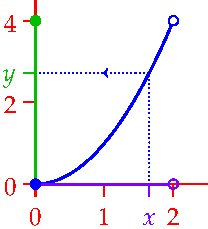
\includegraphics{sets-18-rangedom2}
	  \end{minipage}

% 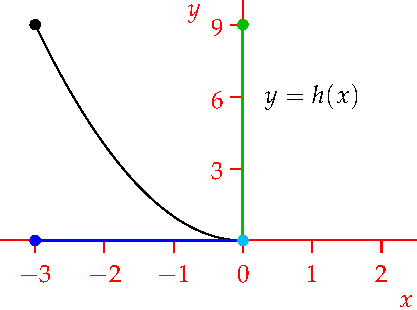
\includegraphics[width=0.4\textwidth]{sets-19-rangedom3}


% 	  \begin{minipage}[t]{0.7\linewidth}\vspace{0pt}
% 	  	\item $f$ is neither injective ($f(a_3)=f(a_4)$) nor surjective $b_4\notin\range(f)$.
% 	  \end{minipage}
% 	  \hfill
% 	  \begin{minipage}[t]{0.29\linewidth}\vspace{0pt}
% 	  	\flushright
% 	  	$\begin{array}{c|cccc}
%   		a&a_1&a_2&a_3&a_4\\\hline
%   		f(a)&b_1&b_2&b_3&b_3
%   		\end{array}$
% 	  \end{minipage}


  	\item $f:\Z\to\{0,1,2\}:n\mapsto n^2\spmod 3$ is neither injective nor surjective.
  	\begin{itemize}
  		\item $f$ is non-injective: for instance $f(1)=f(2)$.
  		\item $f$ is non-surjective: $\range(f)=\{0,1\}\neq \{0,1,2\}=\operatorname{codom}(f)$.
		\end{itemize}
	
		\begin{minipage}[t]{0.64\linewidth}\vspace{-10pt}
    	\item Given $f,g:A\to A$ where $A=\{0,1,\ldots,7\}$ as in the table:
    	\begin{itemize}\itemsep0pt
      	\item $f$ is bijective: all elements of $\operatorname{codom}(f)$ appear exactly once in the $f$-row.
     	 	\item $g$ is non-injective: e.g., $g(0)=g(4)$.
      	\item $g$ is non-surjective: e.g., $1\notin\range(g)=\{0,2,4,6\}$.
    	\end{itemize}
  	\end{minipage}
  	\hfill
  	\begin{minipage}[t]{0.35\linewidth}\vspace{-10pt}
  		\flushright
  		$\begin{array}{c|cccccccccc}
  			n&0&1&2&3&4&5&6&7\\\hline
  			f(n)&0&3&6&1&4&7&2&5\\\hline
  			g(n)&0&6&4&2&0&6&4&2
  		\end{array}$	
  	\end{minipage}

  
	  \item Let $A=\{0,1,2,3,4\}$ and $f:A\to\bigl\{$two-element subsets of $A\bigr\}:a\mapsto \{a,a+1\spmod 5\}$
	  \begin{itemize}%\itemsep0pt
	    \item $f$ is injective: suppose $a_1,a_2\in A$, then
	    \[
	  		f(a_1)=f(a_2)\implies \{a_1,a_1+1\negthickspace\spmod 5\}=\{a_2,a_2+1\negthickspace\spmod 5\}\implies a_1=a_2
	  	\]
	  	\item $f$ is not surjective: e.g., $\{1,3\}\notin\range(f)$.
	  \end{itemize}
    
	\end{enumerate}
\end{examples*}


%To show that a function is bijective, it is enough to exhibit an inverse function. 
You should have seen the approach of the next example in other classes.

\begin{example}[lower separated=false, sidebyside, sidebyside align=top seam, sidebyside gap=0pt, righthand width=0.28\linewidth]{}{}
	We show that $f:(-\infty,2)\to (1,\infty): x\mapsto 1+\frac 1{(x-2)^2}$ is bijective by \emph{computing its inverse function.} Just solve for $x$ in terms of $y$: 
	\begin{align*}
		y=1+\frac 1{(x-2)^2}&\implies (x-2)^2=\frac 1{y-1}\\
		&\implies f^{-1}(y)=x=2-\frac 1{\sqrt{y-1}}
	\end{align*}
	The sign of the square-root was chosen so that $x\in\dom(f)=(-\infty,2)$.
	\tcblower
  \flushright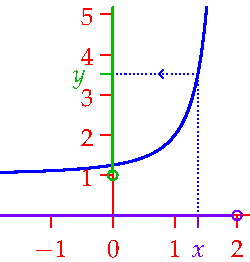
\includegraphics{sets-09-bij2}
\end{example}

\goodbreak

% 
% \begin{aside}{}{}
% {\bf Inverse Functions}
% 
% The word \emph{invertible} is a synonym for bijective because bijective functions really have inverses! Indeed, suppose that $f:A\to B$ is bijective. Since $f$ is surjective, we know that $B=\range(f)$ and so every element of $B$ has the form $f(a)$ for some $a\in A$. Moreover, since $f$ is injective, the $a$ in question is unique. The upshot is that, when $f$ is bijective, we can construct a new \emph{function}
% \[f^{-1}:B\to A:f(a)\mapsto a.\]
% This may appear difficult at the moment but we will return to it in Chapter \ref{chap:relations}.
% 
% Instead, recall that in Calculus you saw that any injective function has an inverse. How does this fit with our definition? Consider, for example, $f:[0,2]\to\R:x\mapsto x^4$. This is injective but not surjective. To fix this, simply define a new function with the same formula but with codomain equal to the range of $f$. We obtain the bijective function
% \[g:[0,2]\to[0,16]:x\mapsto x^4,\]
% with inverse
% \[g^{-1}:[0,16]\to[0,2]:x\mapsto \sqrt[4]{x}.\]
% In Calculus we didn't nitpick like this and would simply go straight to $f^{-1}(x)=\sqrt[4]{x}$.\\[5pt]
% In general, if $f:A\to B$ is any injective function, then $g:A\to f(A):x\mapsto f(x)$ is automatically bijective, since we are forcing the codomain of $g$ to match its range.
% \end{aside}



\boldsubsubsection{Composition of Functions}

We consider how injectivity and surjectivity interact with composition of functions.

\begin{defn}[lower separated=false, sidebyside, sidebyside align=top seam, sidebyside gap=0pt, righthand width=0.4\linewidth]{}{}
	Given functions $f:A\to B$ and $g:B\to C$, their \emph{composition} is the function
	\[
		\textcolor{red}{g\circ f}:A\to C:a\mapsto g\bigl(f(a)\bigr)
	\]
	Note the order: to compute $(g\circ f)(a)$, first apply $f$, then $g$.
	\tcblower
	\flushright
	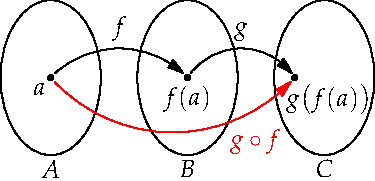
\includegraphics[scale=1]{sets-15-setcomp}
\end{defn}

In practice, some restriction of domains might be required in order to define a composition.

\begin{example}{}{}
	If $f(x)=x^2$ and $g(x)=\frac 1{x-1}$, then
	\[
		(g\circ f)(x)=\frac 1{x^2-1}\quad\text{and}\quad(f\circ g)(x)=\frac 1{(x-1)^2}
	\]
	Even though $\pm 1$ are legitimate inputs for $f$, $\dom(g\circ f) =\R\setminus\{\pm 1\}$ is implied so as to prevent division by zero. 
\end{example}


\begin{thm}{}{compinjsurj}
	Let $f:A\to B$ and $g:B\to C$ be functions. Then:
	\begin{enumerate}
	  \item If $f$ and $g$ are injective, then $g\circ f$ is injective.
	  \item If $f$ and $g$ are surjective, then $g\circ f$ is surjective.
	\end{enumerate}
	It follows that the composition of bijective functions is also bijective.
\end{thm}

\begin{proof}
	Suppose $f$ and $g$ are injective and let $a_1,a_2\in A$. Then
  \begin{align*}
  (g\circ f)(a_1)=(g\circ f)(a_2)&\implies g\big(f(a_1)\big)=g\big(f(a_2)\big)\\
  &\implies f(a_1)=f(a_2)\tag*{(since $g$ is injective)}\\
  &\implies a_1=a_2\tag*{(since $f$ is injective)}\\[-25pt]
  \end{align*}
%   \item Now suppose that $f$ and $g$ are surjective. Let $c\in C$. We are required to show that $\exists a\in A$ such that $(g\circ f)(a)=c$.\\
%   Since $g$ is surjective, $\exists b\in B$ such that $g(b)=c$.\\
%   Similarly, since $f$ is surjective, $\exists a\in A$ such that $f(a)=b$.\\
%   Together we have $(g\circ f)(a)=g(f(a))=c$, as required.
%\end{enumerate}
	That is, $g\circ f$ is injective. We leave part 2 to the exercises.
\end{proof}

Somewhat surprisingly, the converse of this theorem is \emph{false.} If a composition is injective or surjective, \emph{only one} of the original functions is required also to be.

\begin{thm}[lower separated=false, sidebyside, sidebyside align=top seam, sidebyside gap=0pt, righthand width=0.4\linewidth]{}{}
Suppose $f:A\to B$ and $g:B\to C$.
\begin{enumerate}
  \item If $g\circ f$ is injective, then $f$ is injective.
  \item If $g\circ f$ is surjective, then $g$ is surjective.
\end{enumerate}
The picture illustrates what can happen: $f$ is \emph{only injective}, $g$ is \emph{only surjective,} but $g\circ f$ is \emph{bijective.}
	\tcblower
	\flushright
	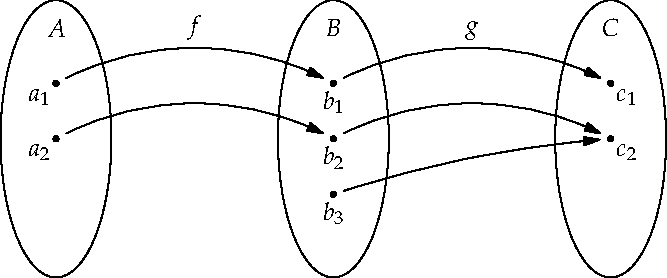
\includegraphics[scale=1]{sets-17-injcomp}
\end{thm}


\goodbreak

\begin{example}{}{}
	Here is a formulaic version of the picture in the theorem. Make sure you're comfortable with the definitions and draw pictures or graphs to help make sense of what's going on.
	\begin{gather*}
		f:[0,2]\to[-4,4]:x\mapsto x^2\tag{injective only}\\
		g:[-4,4]\to [0,16]:x\mapsto x^2\tag{surjective only}\\
		g\circ f:[0,2]\to[0,16]:x\mapsto x^4\tag{bijective!}
	\end{gather*}
\end{example}


\begin{proof}
% \begin{enumerate}\setcounter{enumi}{1}
%   \item Suppose that $f(a_1)=f(a_2)$. Then $(g\circ f)(a_1)=(g\circ f)(a_2)$. Since $g\circ f$ is injective we conclude that $a_1=a_2$, whence $f$ is injective.\qedhere
	This time we leave part 1 for the Exercises. Let $c\in C$ and assume $g\circ f$ is surjective. But then
	\begin{align*}
		&\exists a\in A\text{ such that } c=(g\circ f)(a)=g\bigl(f(a)\bigr)
	\end{align*}
	Otherwise said, $\exists b(=f(a))\in B$ for which $c=g(b)$: that is, $g$ is surjective.%\qedhere
% \end{enumerate}
\end{proof}


\boldsubsubsection{Functions and Cardinality}

Injectivity and surjectivity are intimately tied to the notion of cardinality. In Chapter \ref{chap:cantor}, we will use such functions to \emph{define} cardinality for infinite sets. For the present we stick to finite sets. 

\begin{thm}{}{finitecard}
	Let $A$ and $B$ be finite sets. The following are equivalent:
	\begin{enumerate}\itemsep0pt
	  \item $\nm A\le\nm B$ \qquad\qquad 2. \ $\exists f:A\to B$ injective \qquad\qquad 3. \ $\exists g:B\to A$ surjective
	\end{enumerate}
	Moreover, $\nm A=\nm B\iff\exists f:A\to B$ bijective.
\end{thm}

\begin{minipage}[t]{0.84\linewidth}\vspace{-3pt}
	The theorem asserts that \emph{any one} of the three numbered statements is true if and only if \emph{all} are. It might appear that six arguments are required but, by proving in a circle, we only need three: for instance \circint 1 $\Rightarrow$ \circint 3 holds because \circint 1 $\Rightarrow$ \circint 2 and \circint 2 $\Rightarrow$ \circint 3.\par
	The proof is very abstract, but if you focus on the picture it should make sense.
\end{minipage}
\hfill
\begin{minipage}[t]{0.15\linewidth}\vspace{-3pt}
	\flushright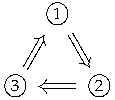
\includegraphics{sets-14-circlearg}%\vspace{-10pt}
\end{minipage}
\par


\begin{proof}
Suppose $\nm A=m$, $\nm B=n$ and label the elements in roster notation:\par
\begin{minipage}[t]{0.63\linewidth}\vspace{-14pt}
\[
	A=\{a_1,a_2,\ldots,a_m\}\qquad B=\{b_1,b_2,\ldots,b_n\}
\]
\begin{description}
	\item[\normalfont \circint 1 $\Rightarrow$ \circint 2]
	If $m\le n$, \emph{define} $f:A\to B$ by $f(a_k)=b_k$ as in the picture. This is injective since the $b_1,\ldots,b_m$ are distinct.
\end{description}
\end{minipage}
\hfill
\begin{minipage}[t]{0.3\linewidth}\vspace{-20pt}
	\flushright
	$\xymatrix @C0pt @R10pt @M1.4pt @H15pt{
		\{a_1, \ar@{|->}[d]_f &a_2,&\ldots,&a_m\} \ar@<-1ex>@{|->}[d]_f\\
		\{b_1, \ar@<-1ex>@{|->}[u]_g &b_2,&\ldots,&b_m, \ar@<0ex>@{|->}[u]_g&\overbrace{b_{m+1},\ldots,b_n}\} \ar@(u,ur)@{|->}@/_3pc/[ullll]_g
	}$
\end{minipage}
\vspace{-2pt}
\begin{description}%\itemsep0pt
	\item[\normalfont \circint 2 $\Rightarrow$ \circint 3] Suppose $f:A\to B$ is injective. Without loss of generality, label the elements of $B$ such that $b_k=f(a_k)$ for $1\le k\le m$. \emph{Define} the surjective function $g:B\to A$ as in the picture:\footnotemark{}%\vspace{-2pt}
  \[
  	g(b_k):=
  	\begin{cases}
  		a_k&\text{ if }k\le m\\
  		a_1&\text{ if }k>m
  	\end{cases}
  \]
  \item[\normalfont \circint 3 $\Rightarrow$ \circint 1] Suppose $g:B\to A$ is surjective. Without loss of generality, label the elements of $B$ such that $a_k=g(b_k)$ for $1\le k\le m$. Since the $b_k$ must be distinct, we see that $n\ge m$.
\end{description}
When $m=n$, the constructed functions are plainly \emph{bijections} with $f^{-1}=g$.
\end{proof}

\vspace{-5pt}

\footnotetext{The elements $b_{m+1},\ldots,b_n$ could be mapped \emph{anywhere,} we choose $a_1$ for simplicity.}

\goodbreak



\begin{exercises}
	A reading quiz and several questions with linked video solutions can be found \href{http://www.math.uci.edu/~ndonalds/math13/selftest/4-3-functions.html}{online}.

	\begin{enumerate}
	  \item For each of the following functions $f:A\to B$ determine whether $f$ is injective, surjective or bijective. Prove your assertions.
	  \begin{enumerate}
	    \item $f:[0,3]\to\R$ where $f(x)=2x$.
	    \item $f:[3,12)\to[0,3)$ where $f(x)=\sqrt{x-3}$.
	    \item $f:(-4,1]\to(-5,-3]$ where $f(x)=-\sqrt{x^2+9}$.
	  \end{enumerate}
	  
	  
	  \item Suppose that $f:[-3,\infty)\to[-8,\infty)$ and $g:\R\to\R$ are defined by
		\[
			f(x)=x^2+6x+1,\qquad\qquad g(x)=2x+3
		\]
		Compute $g\circ f$ and show that it is injective.
	  
	  
	  \item\begin{enumerate}
			\item Find a set $A$ so that the function $f:A\to\R:x\mapsto\sin x$ is injective.
			\item Find a set $B$ so that the function $f:\R\to B:x\mapsto\sin x$ is surjective.
		\end{enumerate}
	

	  \item A function $f:\R\to\R$ is \emph{even} if and only if $\forall x\in\R,\ f(-x)=f(x)$.
		\begin{enumerate}
			\item Prove that $f:x\mapsto x^2$ is even.
			\item By negating the definition, state what it means for a function \emph{not to be even.}
			\item Give an example of a function that is \emph{not} even: prove it. 
			\item Prove or disprove: for every $f,\,g:\R\to\R$ even, the composition $h=f\circ g$ is even.
		\end{enumerate}
		
		
		\begin{minipage}[t]{0.6\linewidth}\vspace{0pt}
			\item The picture in Definition \ref{defn:function1} illustrates a function
			\[
				f:\{a_1,a_2,a_3,a_4\}\to\{b_1,b_2,b_3,b_4\}
			\]
			State the following:\vspace{-2pt}
		\end{minipage}
		\hfill
		\begin{minipage}[t]{0.39\linewidth}\vspace{0pt}
			\flushright
			$\begin{array}{c|cccc}
	   		a&a_1&a_2&a_3&a_4\\\hline
	   		f(a)&b_1&b_2&b_3&b_3
	  	\end{array}$
		\end{minipage}	
		\begin{enumerate}
		  \item $\range(f)$\qquad\qquad (b) \ $f\bigl(\{a_1,a_4\}\bigr)$\qquad\qquad (c) \ $f^{-1}\bigl(\{b_3\}\bigr)$\qquad\qquad (d) \ $f^{-1}\bigl(\{b_4\}\bigr)$
		\end{enumerate}
	
	
		\item\begin{enumerate}
	    \item Let $A=\{a,b,c\}$, $B=\{1,2,3,4\}$ and $f:A\to B$ be the function defined by $f(a)=f(c)=1$ and $f(b)=3$. State the following:
	    	\begin{enumerate}
	    	  \item $f^{-1}\bigl(\{1\}\bigr)$\qquad\qquad (b) \ $f^{-1}\bigl(\{3\}\bigr)$\qquad\qquad (c) \ $f^{-1}\bigl(\{1,3\}\bigr)$\qquad\qquad (d) \ $f^{-1}\bigl(\{2,4\}\bigr)$
	    	\end{enumerate} 
	    \item Let $g:[-1,\infty)\to\R:x\mapsto x^2+2x+1$. Compute $g^{-1}\bigl((0,2]\bigr)$. 
	    \item Let $h:\R\to\R:x\mapsto \sin x$. Find $h^{-1}\bigl(\{-1,1\}\bigr)$. 
		\end{enumerate}
	
		
	  \item Define $f:(-\infty,0]\to\R$ and $g:[0,\infty)\to\R$ by
	  \[
	  	f(x)=x^2,\qquad g(x)=
	  	\begin{cases}
	  		\frac{x}{1-x}&x<1\\
	  		1-x&x\ge 1
	  	\end{cases}
	  \]
	  Is $g\circ f:(-\infty,0]\to\R$ surjective? Justify your answer.
		  
	  
	  \item\label{ex:kfunc} Recall Example \ref*{ex:functions}.\ref{ex:functmod}.
	  Consider the nine functions $f_k:A\to A:x\mapsto kx\pmod{10}$, where $k=1,2,\ldots,9$. Find the range of each $f_k$. Can you find a relationship between $k$ and the cardinality of $\range(f_k)$?
			%\item More generally, let $A=\{0,1,2\ldots,n-1\}$ be the set of remainders modulo $n$. If $f_k:A\to A:x\mapsto kx\spmod n$, conjecture a relationship between $\nm{\range(f_k)}$, $k$ and $n$. You don't need to prove your assertions.
	  
	  
	 	\goodbreak
	 
	  
	  \item Let $f:\R\to\R^+$ be the function defined by $f(x)=e^x$. Explain why the following ``proof'' that $f$ is surjective is incorrect. Then, give a correct proof.  
		\begin{proof}[Proof?]
			Let $e^x\in\R^+$ be arbitrary. Then $f(x)=e^x$. We conclude that $f$ is surjective.
		\end{proof}
		
	
		\item\begin{enumerate}
		  \item Show there is a bijection between $\Z$ and $2\Z$.
			\item Let $S$ be the set of all circles in the plane which are centered at the origin. Find a bijection between $S$ and $\R^+$.
			\item Let $A,B$ be \emph{finite} sets. If $A\subsetneq B$, is it possible for there to be a bijection between $A$ and $B$?
		\end{enumerate}
	
	
	  \item Prove that the composition of two surjective functions is surjective.
	  
	  
	  \item Suppose that $g\circ f$ is injective. Prove that $f$ is injective.
	  
	
	  \item Let $f:A\to B$. Prove the following:
	  \begin{enumerate}
	    \item $f$ is injective if and only if $\forall b\in B,\ f^{-1}\bigl(\{b\}\bigr)$ has \emph{at most} one element.
	    \item $f$ is surjective if and only if $\forall b\in B,\ f^{-1}\bigl(\{b\}\bigr)$ has \emph{at least} one element.
	  \end{enumerate}
	  
	  
		\item Prove that functional composition is associative. That is, if $f:A\to B$, $g:B\to C$, and $h:C\to D$ are functions, then for all $a\in A$ we have
			\[
				\bigl(f\circ(g\circ h)\bigr)(a) = \bigl((f\circ g)\circ h\bigr)(a)
			\]
	  
	  \item Following Theorem \ref{thm:compinjsurj}, the composition of bijective functions $f,g$ is itself bijective. Give a \emph{brief} explanation as to why $(g\circ f)^{-1}=f^{-1}\circ g^{-1}$.
	
		
		\item Let $f:A\to B$ and $X\subseteq A$. Fill in the blanks to complete a proof of the following facts:
		\begin{enumerate}
	  	\item $X\subseteq f^{-1}\bigl(f(X)\bigr)$.\qquad\qquad\qquad (b) \ If $f$ is injective, then $X=f^{-1}\bigl(f(X)\bigr)$.
		\end{enumerate}
		\begin{proof}
			\begin{enumerate}
		  	\item $x\in X\Longrightarrow f(x)\in \underline{\phantom{f(X)}}$. Let $y=f(x)$, then $x\in \underline{\phantom{f^{-1}\bigl(\{y\}\bigr)}} \subseteq f^{-1}\bigl(f(X)\bigr)$.
		  	\item $a\in f^{-1}\bigl(f(X)\bigr) \Longrightarrow \underline{\phantom{f(a)\in f(X)}}$, whence $\exists x\in X$ with $f(a)=f(x)$. By injectivity, \underline{\phantom{$x=a$}}, whence $a\in X$. We conclude that \underline{\phantom{$f^{-1}\bigl(f(X)\bigr)\subseteq X$}}. Combine with part (a) for the result.\qedhere
			\end{enumerate}
		\end{proof}
		
	
		\item Let $f:A\to B$ be a function and let $Y\subseteq B$. Prove the following facts:
		\begin{enumerate}
	    \item $f\bigl(f^{-1}(Y)\bigr) \subseteq Y$.\qquad\qquad\qquad (b) \ If $f$ is surjective, then $f\bigl(f^{-1}(Y)\bigr)=Y$.
		\end{enumerate}
	  
	
	
		\item (Hard)\lstsp Let $f:A\to B$ be a function and $X,Y\subseteq A$.
		\begin{enumerate}
		  \item Prove that $f(X\cap Y)\subseteq f(X)\cap f(Y)$.
		  \item If $f$ is injective, prove that $f(X\cap Y) = f(X) \cap f(Y)$.
		  \item If $f(X\cap Y)=f(X)\cap f(Y)$ for \emph{all} $X,Y\subseteq A$, prove that $f$ is injective.
		\end{enumerate}
		
		
		
	
	%   \item (\emph{If you did Exercise \ref*{sec:quant}.\ref{ex:decreasing} you should find this easy}) Let $X$ be a subset of $\R$. A function $f:X\to\R$ is \emph{strictly increasing} if 
	% 	\[\forall \,a,\, b \in X,\quad a<b \Longrightarrow f(a)<f(b).\]
	% 	For example, the function $f \colon [0,\,\infty)\to \R, \,x \mapsto x^2$  is increasing because 
	% 	\[\forall a,\,b \in  [0,\,\infty) , \quad a<b \Longrightarrow f(a) = a^2< b^2=f(b).\]
	% 		\begin{enumerate}
	% 	  	\item Give another example of a function that is increasing. Draw its graph, and prove that  the function is increasing.  
	% 	  	\item By negating the above definition, state what it means for a function \emph{not to be strictly increasing.} 
	% 	  	\item Give an example of a function that is \emph{not} strictly increasing. Draw its graph, and prove that the function is not strictly increasing.  
	% 	  	\item Let $f,\,g:\R\to\R$ be strictly increasing. Prove or disprove: The function $h=f+g$ is strictly increasing. Note that the formula for $h$ is $h(x)=f(x)+g(x)$.
	% 		\end{enumerate}	
			
	%   \item You may assume that $g:[2,\infty)\to\R:x\mapsto \sqrt{x^3-8}$ is an injective function. Find a function $f:\R\to\R$ which is \emph{not injective,} but for which the composition $f\circ g:[2,\infty)\to\R$ \emph{is injective.} Justify your answer.
	
	% \item Let $f : A \to B$ be a function. Let $X_1,X_2 \subseteq A$. Prove or disprove the following:
	% \begin{enumerate}
	%     \item $X_1 \subseteq X_2$ implies $f(X_1) \subseteq f(X_2)$.
	%     \item $f(X_1 \cup X_2) = f(X_1) \cup f(X_2)$.
	%     \item $f(X_1 \cap X_2) \subseteq f(X_1) \cap f(X_2)$. 
	%     \item $f(X_1) \cap f(X_2) \subseteq f(X_1 \cap X_2)$.
	%     %\item If $f$ is injective, then $f(X_1 \cap X_2) = f(X_1) \cap f(X_2)$.
	%     %\item $f(X_1) \setminus f(X_2) \subseteq f(X_1 \setminus X_2)$.
	% \end{enumerate}
	
% \item Let $f : A \to B$ be a function and $Y_1,Y_2 \subseteq B$.
% \begin{enumerate}
% \item Prove $f^{-1}(Y_1 \cup Y_2) = f^{-1}(Y_1) \cup f^{-1}(Y_2)$.
% \item Prove $f^{-1}(Y_1 \cap Y_2) = f^{-1}(Y_1) \cap f^{-1}(Y_2)$.
% \end{enumerate}



% \item (Uses calculus) This exercise will give an example of how to use calculus to prove some properties of (certain) functions. Let $f : (-\pi/2,\pi/2) \to \R$ be defined by $f(x) = \tan x$. Recall that $f$ is differentiable, and hence continuous, on its domain.
% \begin{enumerate}
%     \item Compute $\lim_{x \to \frac{\pi}{2}^-} f(x)$ and $\lim_{x \to \frac{-\pi}{2}^+} f(x)$.
%     \item Recall the Intermediate Value Theorem: if $g : [a,b] \to \R$ is a continuous function, then for any $y$ between $g(a)$ and $g(b)$, there is $x \in [a,b]$ such that $g(x) = y$. Use the Intermediate Value Theorem and the results of part 1 to prove $f$ is surjective.
%     \item Why is a strictly increasing function (see Exercise 4.4.4) injective? 
%     \item Compute $\frac{d}{dx}f(x)$ and use this to show $f$ is strictly increasing, and therefore injective by part 3.
% \end{enumerate}
	\end{enumerate}

\end{exercises}


%\graphicspath{{5induction/asy/}}
\section{Mathematical Induction and Well-ordering}\label{chap:induction}

In Section \ref{sec:proof} we discussed three methods of proof: direct, contrapositive, and contradiction. The fourth standard method, \emph{induction,} has a very different flavor. Before giving a formal definition, we consider how the need for induction arguments often arises.

\subsection{Iterative Processes \& Proof by Induction}\label{sec:induction}

Recursive processes are very common in mathematics and its applications: an unknown $x_n$ satisfies a simple recurrence relation $x_{n+1}=f(x_n)$ where an initial value $x_1$ is given. The typical approach to such problems is to \emph{hypothesize} a general formula $x_n=g(n)$ (spot a pattern!), and then \emph{prove} the validity of the formula. Induction is the proof method often employed in such situations. To get us started, we investigate a famous game.


\boldsubsubsection{The Tower of Hanoi}

Circular disks of decreasing radius are stacked on three pegs. Disks are moved one at a time from the top of a stack onto an empty peg or on top of a larger disk. If we start with 10 disks on the first peg, how many moves are required to transfer all disks to another peg?\smallbreak

To get a feel for the problem, try playing the game with smaller numbers of disks. Suppose $n$ disks require $r_n$ moves. Then:
\begin{itemize}\itemsep0pt
  \item $r_1=1$ since there is only one disk to move!
  \item $r_2=3$ as shown in the picture.
\end{itemize} 

\begin{center}
	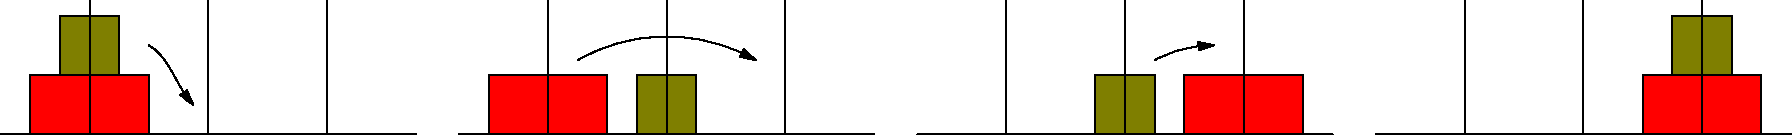
\includegraphics[width=0.9\textwidth]{induction-03-hanoi2}
\end{center}

More experimentation will hopefully convince you that $r_3=7$, at which point you might be ready to hypothesize a general formula---if not, experiment more!

\begin{conj}{}{hanoi}
	The Tower of Hanoi with $n$ disks requires $r_n=2^n-1$ moves.
\end{conj}

To make progress, consider a stack of $n+1$ disks. To move the largest disk, \emph{all other disks must be stacked on a single peg.} Moving $n+1$ disks is therefore a three-step process:
\begin{enumerate}\itemsep0pt
  \item Move the smallest $n$ disks to another peg.
  \item Move the largest disk.
  \item Move the remaining disks on top of the largest.
\end{enumerate}
\begin{center}
\href{http://www.math.uci.edu/~ndonalds/math13/induction-01-hanoi.html}{
	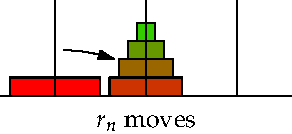
\includegraphics{induction-04-hanoirn3}\quad
	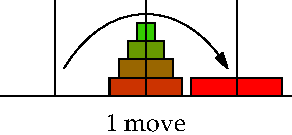
\includegraphics{induction-04-hanoirn4}\quad
	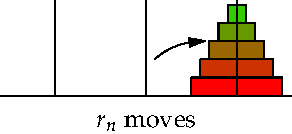
\includegraphics{induction-04-hanoirn5}
}
\end{center}


The upshot is that $r_n$ satisfies a \emph{recurrence relation}: $r_{n+1}=r_n+1+r_n=2r_n+1$.

\goodbreak

We are now in a position to prove our conjecture.

\begin{proof}
	Certainly the formula $r_n=2^n-1$ holds when $n=1$ disk (1 disk requires $r_1=1$ move).\smallbreak
	Now suppose that $n$ disks require $r_n=2^n-1$ moves, where $n\in\N$ is some fixed number. Then $n+1$ disks require
	\[
		r_{n+1}=2r_n+1=2(2^n-1)+1 =2^{n+1}-1
	\]
	moves ($\ast$). Since $n$ was arbitrary, we have in fact proved an \emph{infinite collection of implications}: 
	\[
		r_1=2^1-1\implies r_2=2^2-1\implies r_3=2^3-1 \implies \cdots \implies r_n=2^n-1\implies \cdots
	\]
	Since the first of these propositions ($r_1=2^1-1$) is true, we conclude that $r_n=2^n-1$ for all $n\in\N$.
\end{proof}

To answer the original question, 10 disk require $r_{10}=2^{10}-1=1023$ moves; at one move per second this would take 17 minutes, 3 seconds.



\boldsubsubsection{Proof by Induction}

The Tower of Hanoi argument is an example of \emph{proof by induction.} This method is invoked when we want to prove a sequence of propositions $P(1)$, $P(2)$, $P(3)$, \ldots, one for each natural number. The abstract structure of an induction proof consists of two separate arguments:
\begin{description}%\itemsep0pt
  \item[\normalfont(\emph{Base case})] Prove that $P(1)$ is true.
  \item[\normalfont(\emph{Induction step})] Prove, for each $n\in\N$, that $P(n)\Longrightarrow P(n+1)$. During this phase, $P(n)$ is termed the \emph{induction hypothesis.}
\end{description}
The result is an infinite chain of implications:
\[
	P(1)\implies P(2)\implies P(3)\implies P(4)\implies P(5)\implies \cdots
\]
Since $P(1)$ is true (base case), \emph{all} the remaining propositions $P(2)$, $P(3)$, $P(4)$, \ldots{} are also true.\smallbreak

Re-read the Tower of Hanoi proof; can you separate the base case and induction step? Our presentation was informal since we were only introducing the concept. For a formal argument, a few modifications should be made.

\begin{itemize}
  \item \emph{Set-up} the proof: orient the reader by stating, ``We prove by induction.'' It might also be helpful to spell out the propositions $P(n)$ and to tell the reader what variable ($n$) controls the induction.
  \item Label the \emph{base case} and \emph{induction step} so the reader knows what you are doing!
  \item After the induction step is complete, state your \emph{conclusion.} In the above we would replace everything after ($\ast$) with, ``By mathematical induction, $r^n=2^n-1$ for all $n\in\N$.''
\end{itemize}


Here is a straightforward and famous result, where we write the proof in our new language.

\begin{thm}{}{ind1}
	The sum of the first $n$ positive integers is $\sum\limits_{k=1}^nk=\frac 12n(n+1)$
\end{thm}

You should be familiar with summation notation $\sum\limits_{k=1}^nk=1+2+3+\cdots+n$: if not \emph{ask}!

\goodbreak



\begin{proof}
	We prove by induction. For each $n\in\N$, let $P(n)$ be the proposition $\smash{\sum\limits_{k=1}^nk=\frac 12n(n+1)}$.
	\begin{description}
		\item[\normalfont\emph{Base case} ($n=1$):] \smash{$\sum\limits_{k=1}^1k=1=\frac 121(1+1)$,} says that $P(1)$ is true.
		\item[\normalfont\emph{Induction Step}:] Fix $n\in\N$, and assume that $P(n)$ is true \emph{for this $n$.} We compute the sum of the first $n+1$ positive integers and use our induction hypothesis $P(n)$ to simplify:
	  \begin{align*}
			\sum_{k=1}^{n+1}k&=\textcolor{blue}{\sum_{k=1}^nk}+(n+1)=\textcolor{blue}{\frac 12n(n+1)}+(n+1) \tag{\textcolor{blue}{induction hypothesis}}\\
			&=\left(1+\frac 12n\right)(n+1)=\frac 12(n+2)(n+1)\\
			&=\frac 12(n+1)\bigl[(n+1)+1\bigr]
	  \end{align*}
	Therefore $P(n+1)$ is true.
	\end{description}
	By mathematical induction, we conclude that $P(n)$ is true for all $n\in\N$. That is
	\[
		\forall n\in\N,\quad \sum\limits_{k=1}^nk=\frac 12n(n+1)\tag*{\qedhere}
	\]
\end{proof}

Note how we grouped $\frac 12(n+1)\bigl[(n+1)+1\bigr]$ so that it is obviously the right hand side of $P(n+1)$.\smallbreak

We present several more examples in a similar vein, but done a little faster. As is typical, we don't explicitly introduce the symbol $P(n)$, though you should feel free to continue doing this if you find it helpful. Aim for a layout like these in your formal writing. 


\begin{example}{}{ind3}
	We prove by induction that, for all $n\in\N$,
	\[
		2+5+8+\cdots+(3n-1)=\frac 12n(3n+1) \tag{$\ast$}
	\]
	\begin{description}\itemsep0pt
		\item[\normalfont\emph{Base case} ($n=1$):] The proposition ($\ast$) is trivially true: $2=\frac 12\cdot 1\cdot(3\cdot 1+1)$.
		\item[\normalfont\emph{Induction Step}:] Fix $n\in\N$ and assume ($\ast$) holds for this value of $n$. Then
		\begin{align*}
			\textcolor{blue}{2+5+\cdots+(3n-1)}+[3(n+1)-1]&=\textcolor{blue}{\frac 12n(3n+1)}+3n+2\\
			&=\frac 12(3n^2+7n+4) =\frac 12(n+1)(3n+4)\\
			&=\frac 12(n+1)\bigl[3(n+1)+1\bigr]
		\end{align*}
		which is the required proposition for $n+1$.
	\end{description}
	By mathematical induction ($\ast$) holds for all $n\in\N$.
\end{example}

For brevity we labelled the desired proposition (what we'd have called $P(n)$) by $(\ast)$ so it could be referenced. The structure is similar to Theorem \ref{thm:ind1}: since the goal is to evaluate a sum, the induction step is little more than adding the same thing ($3n+2$) to both sides of the \textcolor{blue}{induction hypothesis}. In fact, the example could have been proved directly by invoking Theorem \ref{thm:ind1}---can you see how?
\medbreak\goodbreak

Our next two examples are a little harder, requiring more creativity to invoke the induction hypothesis. Both could alternatively be proved directly using modular arithmetic (Chapter \ref{chap:gcd}).

\begin{examples}{}{ind2}
	\exstart We prove by induction that $\forall n\in\N$, the integer $17^n-4^n$ is divisible by 13.
	\begin{enumerate}\setcounter{enumi}{1}
		\item[]\begin{description}
			\item[\normalfont\emph{Base case} ($n=1$):] Plainly $17^1-4^1$ is divisible by 13.
			\item[\normalfont\emph{Induction Step}:] Fix $n\in\N$ and assume that $17^n-4^n=13k$ for some $k\in\Z$. Then
			\begin{align*}
				17^{n+1}-4^{n+1}&=17\bigl(\textcolor{blue}{17^n}\bigr)-4^{n+1}=17\bigl(\textcolor{blue}{13k+4^n}\bigr)-4^{n+1} \tag{\textcolor{blue}{induction hypothesis}}\\
				&=17\cdot 13k+(17-4)4^n =13\bigl(17k+4^n\bigr)
			\end{align*}
			is divisible by 13.
		\end{description}
		By mathematical induction, $17^n-4^n$ is divisible by 13 for all $n\in\N$.		
		
		\item\label{ex:ind22} We prove by induction: if $n\in\N$, then $n(n+1)(2n+1)$ is divisible by 6.
		\begin{description}
			\item[\normalfont\emph{Base case} ($n=1$):] The proposition reads $1\cdot (1+1)\cdot (2\cdot 1+1)=6$, which is divisible by 6.
			\item[\normalfont\emph{Induction Step}:] Fix $n\in\N$ and assume that $\textcolor{blue}{n(n+1)(2n+1)=6k}$ for some $k\in\Z$. Then
			\begin{align*}
					(n+1)(n+2)\bigl[2(n+1)+1\bigr]-\textcolor{blue}{6k}&=\textcolor{blue}{(n+1)}\bigl[(n+2)(2n+3)-\textcolor{blue}{n(2n+1)}\bigr]\\
					&=(n+1)\bigl(2n^2+7n+6-(2n^2+n)\bigr) =6(n+1)^2
				\end{align*}
			from which
			\[
				(n+1)\bigl[(n+1)+1\bigr]\bigl[2(n+1)+1\bigr] =6\bigl((n+1)^2+k\bigr)
			\]
			is divisible by 6.
		\end{description}
		By mathematical induction, $n(n-1)(2n-1)$ is divisible by 6 for all $n\in\N$.	
	\end{enumerate}
\end{examples}


\boldinline{Scratch work is your friend!}

Unless things are very simple, you should build an induction argument by starting with some scratch work for the hard part: the \emph{induction step.} If you're stuck, explicitly stating the propositions $P(n)$ and $P(n+1)$ might help you see how to manipulate one into the other. Here are the propositions for Example \ref{ex:ind2}.1:
\begin{quote}
	\begin{tabular}{ll}
	$P(n)$: &$17^n-4^n=13k$ for some integer $k$\\[5pt]
	$P(n+1)$: &$17^{n+1}-4^{n+1}=13l$ for some integer $l$
	\end{tabular}
\end{quote}
Since $17^n$ is common to both, you could try multiplying both sides of $P(n)$ by 17; if you re-read the example, you'll see that this is essentially the induction step! For Example \ref*{ex:ind2}.2, you might try multiplying out the cubic expressions
\[
	n(n+1)(2n+1)\ \text{ and }\ (n+1)(n+2)(2n+3)
\]
and comparing coefficients. Since the leading term in both is $n^3$, the \emph{difference} is quadratic and therefore much easier to think about\ldots\smallbreak

Remember that scratch work isn't a proof; while your scratch work may make perfect sense to you, if a reader cannot follow it without assistance, then it isn't a proof! It is essential, once you think you understand the induction step, to lay out the entire proof cleanly: \emph{set-up, base case, induction step, conclusion.} As an example of what happens when you don't, here is a typical attempt at Example \ref{ex:ind3} by a student who is new to induction:

\begin{tcolorbox}[exstyle]\vspace{-10pt}
	\begin{align*}
		P(n+1)=\hspace{4pt}&2+5+\cdots+(3n-1)+[3(n+1)-1] =\smash{\frac 12}(n+1)\bigl[3(n+1)+1\bigr]\\
		&\frac 12n(3n+1)+(3n+2) =\frac 12(n+1)(3n+4)\\
		&3n^2+n+6n+4 =3n^2+7n+4
	\end{align*}
\end{tcolorbox}

Is this convincing to you? While there are many issues,\footnote{\textbullet\lstsp $P(n)$ There is no \emph{set-up, base case} or \emph{conclusion} and the word \emph{induction} is missing. The argument needs some English!
\begin{itemize}\itemsep0pt
  \item $P(n)$ has not been \emph{defined}. If you don't define it, don't write it!
  \item $P(n+1)$ is a \emph{proposition}: it cannot \emph{equal} a number! Replacing ``$P(n+1)=$'' with ``$P(n+1)\Longleftrightarrow$'' would correct this.
  \item There are no conditional connectives to indicate the logical flow. Moreover, read top to bottom, the argument is essentially $P(n)\wedge P(n+1)\implies T$, rather than the correct induction step $P(n)\implies P(n+1)$.
\end{itemize}} the student's work isn't without merit, since the required calculation is present (left side of 1\st{} line $=$ left side of 2\nd). While helpful as scratch work, a substantial re-write is needed to make this convincing.
\medbreak

We finish this section with a trickier example of this thinking at work.

\begin{example}{}{}
	An \emph{L-shaped tromino} is an arrangement of three squares in an ``L'' shape. We claim:\par
	\begin{minipage}[t]{0.75\linewidth}\vspace{-4pt}
		\begin{quote}
			If \textcolor{Magenta}{any} single square is removed from a $2^n\times 2^n$ square gird, then the remaining grid may be tiled by L-shaped trominos.
		\end{quote}
		\vspace{-6pt}
		The claim has the form $\forall n\in\N,P(n)$, but note that $P(n)$ is itself \textcolor{Magenta}{universal}. The picture shows one of the \emph{sixteen} possible examples when $n=2$. To get an idea of how to structure the induction step, think how you might use $2\times 2$ grids to analyse a $4\times 4$ grid. The picture shows how!
		\begin{itemize}
		  \item Whatever square we remove, one quarter of the $2^2\times 2^2$ grid is a $2^1\times 2^1$ grid with one square removed: this is \textcolor{blue}{tilable}.
		\end{itemize}
	\end{minipage}
	\hfill
	\begin{minipage}[t]{0.24\linewidth}\vspace{0pt}
		\flushright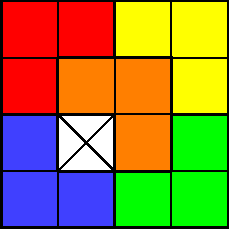
\includegraphics{induction-11-tilingexample}
	\end{minipage}
	\par

\vspace{-2pt}
		
	\begin{itemize}
	 	\item Place a single tromino (yellow in the picture) so that one of its squares lies in each remaining quadrant. What's left of each quadrant is a $2^1\times 2^1$ grid with one missing square: again tilable.
	\end{itemize}
	
	This scratch work is really an argument $P(1)\Longrightarrow P(2)$! It remains only to formalize this intuition into a general proof. We proceed by induction on $n$.
	\begin{description}
		\item[\normalfont\emph{Base case} ($n=1$):] If a single square is removed from a $2\times 2$ grid, the three remaining squares form single L-shaped tromino.
		\item[\normalfont\emph{Induction step}:] Fix $n\in\N$ and assume that after removing \emph{any} square from any $2^n\times 2^n$ grid, the remainder is tilable. Now take any $2^{n+1}\times 2^{n+1}$ grid and remove a square.
	\begin{itemize}
	  \item By the induction hypothesis, the $2^n\times 2^n$ quadrant with the removed square is tilable.
	  \item Place a single tromino in the center so that one of its squares lies in each remaining quadrant. What's left of each quadrant is a $2^n\times 2^n$ grid with one missing square: again tilable by the induction hypothesis.
	\end{itemize}  
	\end{description}
	By induction, we conclude that every $2^n\times 2^n$ grid is tilable by trominos after any square is removed.
\end{example}


\goodbreak

\begin{exercises}{}{}
	A reading quiz and several questions with linked video solutions can be found \href{http://www.math.uci.edu/~ndonalds/math13/selftest/5-1-induction.html}{online}.

	\begin{enumerate}
	  \item Suppose you can move one disk on the Tower of Hanoi per second.
	  \begin{enumerate}
	    \item One of the oldest versions of the problem has monks transferring a tower of 64 disks. Roughly how many years would this take?
	    \item In a realistic human lifetime, how large a tower could be moved?
	  \end{enumerate}
	  
	  
	  \item Imagine you cut a large large piece of paper in half and stack the two pieces on top of each other. You then repeat the process, cutting all sheets in half and making a single taller stack.
		\begin{center}
			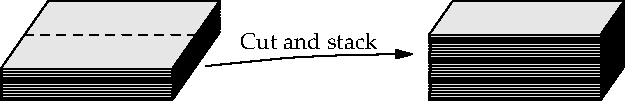
\includegraphics{induction-02-paper}
		\end{center}
		If a single sheet of paper has thickness $0.1$\,mm, how many times would you have to repeat the cut-and-stack process until the stack of paper reached to the sun? ($\approx 150$ million kilometers). \emph{Prove} that you are correct.
	  
	
	  \item A room contains $n$ people. Everybody wants to shake everyone else's hand (but not their own).
	  \begin{enumerate}
	    \item Suppose $n$ people require $h_n$ handshakes. If person $n+1$ enters the room, how many \emph{additional} handshakes are required? Obtain a recurrence relation for $h_{n+1}$ in terms of $h_n$.
	    \item Hypothesize a general formula for $h_n$, and prove it by induction.
	  \end{enumerate}
	  
	  
	  \item\begin{enumerate}
	    \item In Example \ref*{ex:ind2}.\ref{ex:ind22}, what is the proposition $P(n+1)$?
	    \item In the induction step of Example \ref*{ex:ind2}.\ref{ex:ind22}, explain why it would be incorrect to write
	    \begin{align*}
				P(n+1)-P(n)&=(n+1)\bigl[(n+2)(2n+3)-n(2n+1)\bigr]\\
				&=(n+1)(2n^2+7n+6-2n^2-n)\\
				&=6(n+1)^2
			\end{align*}
			\item Extend the Example by proving, by induction, that $\sum\limits_{k=1}^nk^2=\frac 16n(n+1)(2n+1)$.
	  \end{enumerate}
  
  
	  \item Prove by induction that for each natural number $n$, we have $\smash{\sum\limits_{k=0}^n2^k=2^{n+1}-1}$.
		
		
		\item Consider the statement: If $n$ is a natural number, then $\smash{\sum\limits_{k=1}^nk^3=\frac 14n^2(n+1)^2}$
		\begin{enumerate}
		  \item What, explicitly, is $\smash{\sum\limits_{k=1}^4k^3}$?
		  \item What would be meant by the expression $\smash{\sum\limits_{k=1}^nn^3}$, and why is it different to $\smash{\sum\limits_{k=1}^nk^3}$?
		  \item Proof the statement by induction.
	  \end{enumerate}
	
	
  	\item\begin{enumerate}
    	\item Prove by induction that $\forall n\in\N$ we have $3\mid(2^n+2^{n+1})$.
    	\item Give a direct proof that $3\mid(2^n+2^{n+1})$ for all integers $n\ge 1$.
  	\end{enumerate}

  
		\item Prove \emph{by induction} that for every $n\in\N$ we have $n\equiv 5$ or $n\equiv 6$ or $n\equiv 7\spmod 3$.
	
		\item Prove by induction that, for all $n\in\N$,
		\[
			1\cdot 2+2\cdot 3+3\cdot 4+\cdots +n(n+1) =\frac 13n(n+1)(n+2)
		\]

		\item\begin{enumerate}
		  \item Show, by induction, that for all $n\in\N$, the number 4 divides the integer $11^n-7^n$.
			\item More generally, prove by induction that $(a-b)\mid (a^n-b^n)$ for any $a,b,n\in\N$.
		\end{enumerate}
	
		
		\item\begin{enumerate}
		  \item Find a formula for the sum of the first $n$ odd natural numbers. Prove your assertion.
		 	\item Use Theorem \ref{thm:ind1} to give an alternative direct proof of your formula.
		\end{enumerate} 
  

		\item Find the error in the following ``proof'' of the statement, ``All cats have the same color fur.''
		\begin{proof}
	    Let $P(n)$ be the proposition, ``Any set of $n$ cats have the same color fur.'' We prove by induction on $n$. 
	    \begin{description}\itemsep0pt
	    	\item[\normalfont\emph{Base case} ($n=1$):] Any cat has the same color fur as itself.
	    	\item[\normalfont\emph{Induction step}:] Fix $n\in\N$ and assume $P(n)$. Take any set $S= \{C_1,C_2,\ldots,C_{n+1}\}$ of $n+1$ cats. The set $S\setminus\{C_1\}$ has $n$ cats; by the induction hypothesis all have the same color fur. Again by the induction hypothesis, all cats in $S\setminus\{C_2\}$ have the same color fur. Combining these observations, we see that all cats in $S$ have the same color fur. Since $S$ was arbitrary, we see that $P(n+1)$ holds.
	    \end{description}
	    By induction, $P(n)$ is true for all $n\in\N$, which establishes the claim.
		\end{proof}

		\item Use induction, the product rule, and the fact that $\diff xx=1$ to prove the power law from calculus:
		\[
	    \forall n\in\N,\ \diff x x^n =nx^{n-1}
		\]


		\item A (real) \emph{polynomial} of degree $n$ is a function $p(x)=a_nx^n+a_{n-1}x^{n-1}+ \cdots +a_1x+a_0$, whose \emph{coefficients} $a_k$ are real numbers and where $a_n\neq 0$.
		\begin{enumerate}
    	\item Prove: for all $n\in\N$,
    	\[
        \diff[{}^n]{x^n} e^{x^2} = p_n(x) e^{x^2}
    	\]
    	where $p_n(x)$ is some polynomial of degree $n$.

			\item (Hard)\lstsp Let $p(x)$ be a polynomial of degree $n\ge 1$. Show $p$ has at most $n$ roots.\par
			(\emph{Hint: induct on the degree $n$})
		\end{enumerate}


		\item Consider the following scratch work. Determine what result is being proved, then convert the scratch work into a formal proof of that result.
	  \begin{align*}
	    (1+x)^{n+1}&=(1+x)^n(1+x)\ge (1+nx)(1+x)\\
	    &=1+x+nx+nx^2=1+(n+1)x+nx^2\\
	    &\ge 1+(n+1)x
	  \end{align*}

	\end{enumerate}

\end{exercises}

\clearpage



\subsection{Well-ordering and the Principle of Mathematical Induction}\label{sec:wellorder}


In this section we think more carefully about the logic behind induction, by tying it to a fundamental property of the natural numbers.

\begin{defn}{}{wellorder}
	A non-empty set of real numbers $A$ is \emph{well-ordered} if every non-empty subset of $A$ contains a minimum element.
\end{defn}

To test if a set $A$ is well-ordered, we need to check \emph{all} of its non-empty subsets. The definition could be written as equivalently as follows, where in the second line we expand what is meant by a \emph{minimum}:
\begin{itemize}
  \item $\forall B\subseteq A$ such that $B\neq\emptyset$, $\min B$ exists.
  \item $\forall B\subseteq A$, $B\neq\emptyset\implies \exists b\in B$ such that $\forall x\in B$, $b\le x$.
\end{itemize}
To show that $A$ is \emph{not} well-ordered, we need only exhibit a non-empty subset $B$ with \emph{no minimum.}

\begin{examples}{}{}
	\exstart $A=\{4,-7,\pi,19,\ln 2\}$ is a well-ordered set. There are 31(!) non-empty subsets of $A$, each of which has a minimum element.\vspace{-5pt}
	\begin{enumerate}\setcounter{enumi}{1}
	  \item[] Can you justify this fact \emph{without} listing the subsets? It might be easier to think about why any \emph{finite} set $A=\{a_1,\ldots,a_n\}\subseteq\R$ is well-ordered\ldots 
	  
	  \item The interval $A=[3,10)$ is not well-ordered. Indeed $B=(3,4)$ is a non-empty subset which has no minimum element. While you should believe this, let's prove it anyway!\par
	  We need to prove that $\forall b\in B, \exists x\in B$ with $x<b$. Given any $b\in(3,4)$, observe that $x:=\frac{b+3}2$ satisfies
	  \[
	  	3<x<b<4 \quad\text{from which}\quad x\in B\text{ and }x<b
	  \]
	  You could also argue by contradiction (if $b\in B$ is $\min B$, then\ldots).
	  
	  \item The integers $\Z$ are not well-ordered. For instance, $\Z$ is a non-empty subset of itself and there is no minimum integer.
	\end{enumerate}
\end{examples}

You might suspect (wrongly!) that every well-ordered set is finite. That the natural numbers form a well-ordered \emph{infinite} set is, for us, an axiom:
\footnote{There are many ways to define the natural numbers. Typically well-ordering is either an axiom (essentially part of the definition) or a theorem. Compare with Exercise \ref{exs:peano} for an alternative approach.} a foundational claim that forms part of our basic conception of the natural numbers.

\begin{axiom}{Well-ordering Principle}{}
	$\N$ is well-ordered.
\end{axiom}


Also known as the \emph{least natural number principle}, the well-ordering principle is used repeatedly in mathematics. In fact we've already done so in this text! Consider the set of positive remainders generated by the Euclidean algorithm (Theorem \ref{thm:euclidalg}) applied to $a>b\in\N$:
\[
	\{\ldots,r_2,r_1,b,a\}\subseteq\N
\]
Well-ordering guarantees that this set has a minimal element $r_t$ (which turns out to be $\gcd(a,b)$); this is essentially the argument for Exercise \ref*{sec:gcd}.\ref{exs:euclidalgproof}(a).

\goodbreak  

%  When written in roster notation in increasing order, any set that `looks like' $\N$, is also well-ordered. For example
% \[
% 	A=\left\{0,\frac 12,\frac 23,\frac 34,\frac 45,\ldots\right\}=\left\{\frac n{n+1}:n\in\N\right\}
% \]
Armed with this axiom, we can justify the method of proof by induction. 

\begin{thm}{Principle of Mathematical Induction}{ind}
	For each $n\in\N$, let $P(n)$ be a proposition. Additionally make the two standard assumptions for induction:
	\begin{quote}
		\begin{tabular}{@{}ll}
			\emph{Base case}: &$P(1)$ is true\\[5pt]
			\emph{Induction step}: &$\forall n\in\N,\ P(n)\Longrightarrow P(n+1)$
		\end{tabular}
	\end{quote}
	Then $P(n)$ is true for all $n\in\N$.
\end{thm}

Before attempting a proof, consider how the theorem could be written as a pure implication:
\[
	\textcolor{blue}{P(1)\wedge\bigl(\forall n\in\N,P(n)\Longrightarrow P(n+1)\bigr)}\Longrightarrow \textcolor{Green}{\bigl(\forall n\in\N, P(n)\bigr)}
\]
This helps us select a proof strategy: a direct approach seems hard since the \textcolor{Green}{conclusion} is universal; a contrapositive approach requires an ugly negation of the \textcolor{blue}{hypothesis}; a proof by contradiction seems most sensible since negation of the \textcolor{Green}{conclusion} is straightforward.

\begin{proof}
	We argue by contradiction. Assume the base case, the induction step, and that $\exists n\in\N$ for which $P(n)$ is \emph{false.} The set of natural numbers
	\[
		S:=\bigr\{k\in\N:P(k)\text{ is false}\bigr\}
	\]
	is non-empty (since $n\in S$). Well-ordering guarantees that $s:=\min S$ exists. Observe:
	\begin{itemize}\itemsep0pt\parskip2pt
	  \item $s\in S\Longrightarrow$ \textcolor{red}{$P(s)$ is \emph{false}}.
	  \item The \emph{base case} tells us that $s\neq 1$, whence $s-1\in\N$.
	  \item $s-1<\min S\implies P(s-1)$ is \emph{true.}
	  \item The \emph{induction step} ($P(s-1)\Longrightarrow P(s)$) tells us that \textcolor{red}{$P(s)$ is \emph{true}}.
	\end{itemize}
	\textcolor{red}{Contradiction}: $P(s)$ cannot be both true and false!
\end{proof}


Now we have the proof, it is straightforward to extend the principle of induction. For any integer $m$ (positive, negative or zero), the set
\[
	\Z_{\ge m}=\{n\in\Z:n\ge m\}=\{m,m+1,m+2,m+3,\ldots\}
\]
is also well-ordered. By changing the base case to $P(m)$ and replacing $\N$ with $\Z_{\ge m}$, we immediately obtain the proof of a more general principle of induction.

\begin{cor}{Induction with base case $m$}{indbasem}
	Fix an integer $m$. For each integer $n\ge m$, let $P(n)$ be a proposition. Suppose:
	\begin{quote}
		\begin{tabular}{@{}ll}
			\emph{Base case}: &$P(m)$ is true\\[5pt]
			\emph{Induction step}: &$\forall n\in\Z_{\ge m},\ P(n)\Longrightarrow P(n+1)$
		\end{tabular}
	\end{quote}
	Then $P(n)$ is true for all $n\in\Z_{\ge m}$.
\end{cor}

The intuitive concept is exactly as before, just with a different base case!
\[
	P(m)\implies P(m+1)\implies P(m+2)\implies P(m+3)\implies\cdots
\]
\goodbreak

% As long as you explicitly prove the first claim in the sequence, and you show the induction step, then all the propositions are true.\par



\begin{examples}{}{}
	\exstart For all integers $n\ge 2$, we have\footnotemark
	\[
		\sum\limits_{k=2}^n\frac 1{k(k-1)} =1-\frac 1n\tag{$\ast$}
	\]	
	\begin{enumerate}\setcounter{enumi}{1}
		\item[]\begin{description}
			\item[\normalfont\emph{Base case} ($n=2$):] When $n=2$, ($\ast$) reads $\smash{\sum\limits_{i=2}^2}\frac 1{i(i-1)}=\frac 12=1-\frac 12$.
			\item[\normalfont\emph{Induction step}:] Assume that ($\ast$) is true for some fixed $n\ge 2$. Then
			\begin{align*}
				\sum_{i=2}^{n+1}\frac 1{k(k-1)} &=\sum_{i=2}^{n}\frac 1{k(k-1)}+\frac 1{(n+1)n} =1-\frac 1n+\frac 1{n(n+1)}\tag{induction hypothesis}\\
				&=1-\frac{(n+1)-1}{n(n+1)} =1-\frac 1{n+1}
			\end{align*}
			which is exactly ($\ast$) when $n$ is replaced by $n+1$.
		\end{description}
		By induction ($\ast$) holds for all integers $n\ge 2$.
	
	  \item For all integers $n\ge 4$, we claim that $3^n>n^3$.\par
	  We really need a different base case: when $n=3$, the claim $3^3>3^3$ is false! As is often the case, it helps to do some scratch work first. The \textcolor{blue}{induction hypothesis} allows us to see that 
	  \[
	  	3^{n+1}=3\cdot \textcolor{blue}{3^n} >3 \textcolor{blue}{n^3}
	  \] 
	  The proof of the induction step therefore hinges on being able to show that $3n^3\ge (n+1)^3$. There are many ways to convince yourself of this: for instance
	  \[
	  	3n^3\ge(n+1)^3\iff 3\ge\left(\frac{n+1}n\right)^3 =\left(1+\frac 1n\right)^3 \tag{$\dag$}
	  \]
	  The right side \emph{decreases} as $n$ increases; since $n\ge 4$, the right side is at most $\left(\frac 54\right)^3=\frac{125}{64}<2$, whence ($\ast$) holds for all $n\ge 4$.\smallbreak
	  
	  We now prove the original claim by induction.	  
	  \begin{description}
	  	\item[\normalfont\emph{Base case} ($n=4$):] Observe that $3^4=81>64=4^3$.
	  	\item[\normalfont\emph{Induction step}:] Fix $n\in\Z_{\ge 4}$ and suppose that $3^n>n^3$. By ($\dag$), we see that
			\[
				3^{n+1}=3\cdot 3^n>3n^3\ge (n+1)^3
			\]
	  \end{description}
	  By induction, we conclude that $3^n>n^3$ whenever $n\in\Z_{\ge 4}$.
	\end{enumerate}
\end{examples}


\footnotetext{You might have encountered this example as a \emph{telescoping series} in calculus:
\[
	\sum\limits_{k=2}^n\frac 1{k(k-1)}=\frac 1{2\cdot 1}+\frac 1{3\cdot 2}+\cdots +\frac 1{n(n-1)} =\left(1-\frac 12\right) +\left(\frac 12-\frac 13\right) +\cdots +\left(\frac 1{n-1}-\frac 1n\right) =1-\frac 1n
\]
In calculus, you'd take the limit as $n\to\infty$ to obtain the infinite series $\sum\limits_{k=2}^\infty\frac 1{k(k-1)}=1$}


As a final example, we prove an extended version of de Morgan's law for sets (Theorem \ref{thm:setcomp}(a)).

\begin{example}{}{}
	For any collection of sets $A_1,\ldots,A_n$ where $n\ge 2$, we have
	\[
	 	\comp{(A_1\cap \cdots\cap A_n)}=\comp{A_1}\cup\cdots\cup\comp{A_n} \tag{$\ddag$}
	\]
	\begin{description}
		\item[\normalfont\emph{Base case} ($n=2$):] $\comp{A_1\cap A_2}=\comp{A_1}\cup\comp{A_2}$ is precisely the standard de Morgan identity.
		\item[\normalfont\emph{Induction step}:] Fix $n\in\N_{\ge 2}$ and suppose ($\ddag$) holds for \emph{all} collections of $n$ sets. Given a collection of $n+1$ sets, we see that
		\begin{align*}
			\comp{(A_1\cap \cdots\cap A_n\cap A_{n+1})} &=\comp{\bigl((A_1\cap \cdots\cap A_n)\cap A_{n+1}\bigr)}\\
			&=\comp{(A_1\cap \cdots\cap A_n)}\cup \comp{A_{n+1}} \tag{de Morgan again!}\\
			&=\comp{A_1}\cup\cdots\cup\comp{A_n}\cup\comp{A_{n+1}} \tag{induction hypothesis}
		\end{align*}
	\end{description}
	By induction the claim ($\ddag$) holds for any collection of $n$ sets.
\end{example}

We could have approached the argument as a standard induction with base case $n=1$. Instead we deliberately chose the base case $n=2$, both to avoid confusion (the trivial $\comp{A_1}=\comp{A_1}$ isn't helpful or interesting) and to highlight the importance of de Morgan's law for two sets to the entire argument.

\boldsubsubsection{Proof by Minimal Counter-example}

Sometimes authors present induction arguments as contradiction proofs in line with Theorem \ref{thm:ind}: the element $s=\min S$ is known as the \emph{minimal counter-example.} Here are two variations on this idea; the first is a straight translation of an induction where the base case and induction step are clear.

\begin{examples}{}{}
	\exstart We prove: for all $n\in\N_0$, $\sum\limits_{k=0}^n 2^k=2^{n+1}-1$.\vspace{-10pt}
	
	\begin{enumerate}\setcounter{enumi}{1}
	  \item[]Suppose to the contrary and let $s\ge 0$ be the minimal counter-example.
	  \begin{itemize}
	    \item Since $\smash{\sum\limits_{k=0}^0} 2^k=2^0=1=2^{0+1}-1$, we see that $s\neq 0$.\hfill (\emph{base case})
	    \item But then
	    \[
	    	\sum\limits_{k=0}^s2^k=2^s+\sum\limits_{k=0}^{s-1} 2^k =2^s+2^s-1=2^{s+1}-1 \tag{\emph{induction step}}
	    \]
	    contradicts the fact that $s$ is a counter-example!
	  \end{itemize} 
	  
	  
	  \item We re-prove Theorem \ref{thm:sqrt2}: $\sqrt 2\notin\Q$. Suppose $\sqrt 2$ is rational and consider the set
	  \[
	  	S=\bigl\{x\in\N:\exists y\in \N\text{ with }x^2=2y^2\bigr\}
	  \]
	  Let $s=\min S$ and $t\in\N$ be such that $s^2=2t^2$: plainly $\textcolor{red}{t<s}$. Since $s^2$ even $\Longrightarrow s$ even, we can write $s=2k$, from which
	  \[
	  	4k^2=2t^2\implies n^2=2k^2\implies \textcolor{red}{t\in S}
	  \]
	  This contradicts the minimality of $m$.\par
	  This approach is often used in number theory in the guise of Fermat's \emph{method of infinite descent.}
	\end{enumerate}
\end{examples}



\begin{aside}{}{}
	\boldinline{Aside: Well-ordering more generally}

	Definition \ref{defn:wellorder} is a weak version of a much deeper concept. Informally, to \emph{well-order} a set means to list its elements in some order so that every non-empty subset has an initial element \emph{with respect to that order.}\par
	For instance, the set of negative integers $\Z^-=\{\ldots,-4,-3,-2,-1\}$ is \emph{not} well-ordered with respect to the standard ordering of the integers, but is well-ordered with respect to the \emph{reverse} ordering
	\[
		\Z^-=\{-1,-2,-3,-4,\ldots\}
	\]
	The principle of mathematical induction is easily modified to accommodate theorems of the form $\forall n\in\Z^-,\ P(n)$: the base case is $P(-1)$ and the induction step justifies the chain
	\[
		P(-1)\implies P(-2)\implies P(-3)\implies\cdots
	\]
	All the infinite well-ordered sets we've thus far seen have ``looked like'' the natural numbers, however more esoteric examples exist. For instance, the following well-ordered set looks like two copies of the natural numbers, one following the other:
	\[
		A=\left\{0,\frac 12,\frac 23,\frac 34,\frac 45,\ldots,1,\frac 32,\frac 53,\frac 74,\frac 95,\ldots\right\}=\left\{1-\frac 1n:n\in\N\right\}\cup\left\{2-\frac 1n:n\in\N\right\}
	\]
	Every non-empty subset of $A$ really does have a minimum!	It is possible to modify induction to apply to propositions indexed by well-ordered sets like this, though an extra step is required to deal with \emph{limit elements} (like $1\in A$) with no immediate predecessor. If your further studies include set theory, you'll likely spend much time considering well-orders and their associated \emph{ordinals.}
\end{aside}


\begin{exercises}
	A reading quiz and several questions with linked video solutions can be found \href{http://www.math.uci.edu/~ndonalds/math13/selftest/5-2-wellorder.html}{online}.

	\begin{enumerate}
  	\item Prove that the interval $(-2,5]$ has no minimum element.
	
	
		\item Prove that every finite set of real numbers is well-ordered.
  
  
  	\item\begin{enumerate}
    	\item Suppose that $n\ge 3$. Prove that $\left(\frac{n+1}n\right)^2<2$.
    	\item Hence or otherwise, prove that $n^2<2^n$ for all natural numbers $n\ge 5$.
  	\end{enumerate}
  	

	  \item Consider the following result. For every natural number $n\ge 2$,
		\[
			\left(1-\frac{1}{4}\right) \left(1-\frac{1}{9}\right) \left(1-\frac{1}{16}\right) \cdots \left(1-\frac{1}{n^2}\right) = \frac{n+1}{2n}
		\]
	  \begin{enumerate}
	    \item If the statement is written in the form $\forall n\in\N_{\ge 2},\ P(n)$, what is the proposition $P(n)$?
% 	    \item $\Pi$-notation is used for products in the same way as $\Sigma$-notation for sums: for example
% 	    \[\prod_{k=1}^5(k+1)^k=2^1\cdot 3^2\cdot 4^3\cdot 5^4\cdot 6^5\]
% 	    Rewrite the statement using $\Pi$-notation.
	    \item Prove the result by induction.
	  \end{enumerate}
	  
	  
	
		\item Prove the geometric series formula: if $r\neq 1$ and $n\in\N_0$, then
			$\smash{\sum\limits_{k=0}^n}r^k=\frac{1-r^{n+1}}{1-r}$
			
		
		\item For all integers $n\ge 3$, prove that $\smash{\sum\limits_{k=3}^n}\frac 1{k(k-2)} =\frac 34-\frac{2n-1}{2n(n-1)}$	
		
		
		\item Prove: for any $n\in\N$, $\smash{\sum\limits_{i=1}^n}\frac{1}{i^2}<2$\par
	(\emph{Hint: prove the stronger fact that $\smash{\sum\limits_{i=1}^n} \frac{1}{i^2} < 2 - \frac{1}{n}$ for all $n \ge 2$})
	
	
		\goodbreak
		
	
  	\item The set $A_3=\{1,2,3\}$ satisfies the property that the sum of its elements ($1+2+3=6$) is divisible by every element of $A_3$.
  	\begin{enumerate}
  	  \item Use induction to prove that for any $n\ge 3$, there is a set $A_n$ of $n$ natural numbers such that the sum of its elements is divisible by every element of $A_n$.
  	  \item Prove by contradiction that no set of \emph{two} natural numbers satisfies this property.
  	\end{enumerate}
 	
	
		\item Suppose that $x^2+4y^2=3z^2$ has a solution $(x,y,z)$ where all three are \emph{positive integers.}
		\begin{enumerate}
	  	\item By considering remainders modulo 3, prove that $3\mid z$. Thus create a new solution $(X,Y,Z)$ in positive integers, where $Z<z$.
	  	\item Use the method of minimal counter-example to prove that $x^2+4y^2=3z^2$ has no solutions where $x,y,z\in\N$.
		\end{enumerate}
  
	
		\item We use the fact that $\N_0$ is well-ordered to prove the division algorithm (Theorem \ref{thm:div}).
		\begin{quote}
			\emph{If $m\in\Z$ and $n\in\N$, then $\exists$ unique $q,r\in\Z$ such that $m=qn+r$ and $0\le r<n$.}
		\end{quote}
	
		Given $m,n$, define
		\[
			S=\N_0\cap\bigl(m+n\Z\bigr) =\bigl\{k\in\N_0:k=m-qn\text{ for some } q\in\Z\bigr\}
		\]	
		\begin{enumerate}
			\item (Existence)\lstsp Show that $S$ is a \emph{non-empty} subset of $\N_0$. By well-ordering, \emph{define} $r:=\min S$. Prove that $0\le r<n$.
			\item (Uniqueness)\lstsp Suppose two pairs of integers $(q_1,r_1)$ and $(q_2,r_2)$ satisfy $m=q_in+r_i$ and $0\le r_1,r_2<n$. Prove that $r_1=r_2$.
		\end{enumerate}
		
	
	  \item\label{exs:peano} (Hard)\lstsp We consider a version of Peano's axioms for the natural numbers.
		\begin{itemize}
			\item[i.] (\emph{Initial element})\lstsp $1\in\N$
			\item[ii.] (\emph{Successor function})\lstsp $f(n)=n+1$ is a function $f:\N\to\N$
			\item[iii.] (\emph{No predecessor of the initial element})\lstsp $1\not\in\range(f)$
			\item[iv.] (\emph{Unique predecessor/order})\lstsp $f$ is injective: $m+1=n+1\Longrightarrow m=n$
			\item[v.] (\emph{Induction})\lstsp Any subset $A\subseteq\N$ with the following properties \emph{equals} $\N$:
			\[
				1\in A\quad\text{and}\quad \forall a\in A,\ a+1\in A
			\]
		\end{itemize}
		\begin{enumerate}
			\item Replace $\N$ with $\Z$ in each axiom. Which are true and which false?
			\item Let $T=\bigl\{(m,n):m,n\in\N\bigr\}$ be the set of all ordered pairs of natural numbers.
			\begin{enumerate}
			  \item Let $f:T\to T$ be the function $f(m,n)=(m+1,n)$. Letting the pair $(1,1)$ play the role of 1, and $f$ the successor function, decide which of Peano's axioms are satisfied by $T$.
				\item Repeat the question for the same initial element and 
				\[
					f:T\to T:(m,n)\mapsto
					\begin{cases}
						(m-1,n+1)&\text{if }m\ge 2\\
						(m+n,1)&\text{if }m=1
					\end{cases}
				\]
			\end{enumerate}
			\item Prove that $\range(f)=\N\setminus\{1\}$: every element except 1 is the successor of something.\par
			(\emph{Hint: let $A=\{1\}\cup\range(f)$ in the induction axiom})
			\item Prove that $\N$, as defined by Peano, is well-ordered (with respect to $x<x+1$, etc.).
		\end{enumerate}

	\end{enumerate}

\end{exercises}


% The induction arguments in the above examples are so simple that they hardly seem worth mentioning. In other situations things can be much harder.\\
% Bob
% 
% \begin{example}
% Recall the monotone convergence theorem from sequences. If $(x_n)$ is an increasing (decreasing) sequence bounded above (below), then it is convergent. Here we use this theorem to prove that the following sequence converges to $\frac 12$:
% \[\begin{cases}
% x_{n+1}=\frac 13(x_n+1)+(x_n-\tfrac 12)^2,\\
% x_1=1.
% \end{cases}\]
% You can try hunting for a general formula for $x_n$ (if you find one, let us know\ldots). Instead we observe the first few terms of the sequence: $(x_n)=(1,\frac{11}{12},\frac{13}{16},\frac{539}{768},\ldots)$ and hypothesize:\\[10pt]
% Conjecture:\quad $(x_n)$ is a decreasing sequence and $x_n>\frac 12$ for all $n\in\N$.\\
% We prove by induction.\\
% Certainly $x_1=1>\frac 12$. Now if $x_n>\frac 12$, we have $x_n-\frac 12\neq 0$, whence
% \[x_{n+1}>\frac 13\left(x_n+1\right)>\frac 13\left(\frac 12+1\right)=\frac 13\cdot\frac 32=\frac 12.\]
% Thus all $x_n>\frac 12$ by induction.\\[10pt]
% Given this, we can now see that
% \[x_{n+1}-x_n=\frac 13(1-2x_n)-\left(x_n-\frac 12\right)^2<0,\]
% thus $(x_n)$ is decreasing. Since $(x_n)$ is also bounded below (by $\frac 12$), the monotone convergence theorem says that the sequence converges.\\
% Call the limit $x$. Clearly $x\ge 1$. But then
% \[x=\frac 13(x+1)+\left(x-\frac 12\right)^2\iff x=\frac 12\text{ or }\frac 76.\]
% Since $(x_n)$ is decreasing from 1, it is clear that $\lim_{n\to\infty}x_n=\frac 12$.\\
% Note that it is essential that we establish the existence of the limit before calculating it: the same sequence but with initial value $x_1=2$ is \emph{divergent} to $\infty$.
% \end{example}

% Our final example involves a little abstraction.
% 
% \begin{thm}{}{polygon}
% 	The interior angles of an $n$-gon ($n$-sided polygon) sum to $180(n-2)$ degrees.
% \end{thm}
% 
% We will take the initial case ($n=3$) that the angles of a triangle sum to \ang{180} as given (can you prove it?) and merely prove the induction step. The main logical difficulty is that we must consider \emph{all} $n$-gons simultaneously. If we were to write the induction step in the form
% \[
% 	\forall n\in\Z_{\ge 3},\ P(n)\implies P(n+1)
% \]
% then the proposition $P(n)$ would be
% \[
% 	P(n):\quad \forall n\text{-gons }\cP_n,\text{ the sum of the interior angles of $\cP_n$ is $180(n-2)$\textdegree}
% \]
% To prove our induction step for a \emph{fixed} integer $n$, we must show that \emph{all} $(n+1)$-gons have the correct sum of interior angles. We therefore assume that we are given some $(n+1)$-gon $\cP_{n+1}$ and proceed to compute its interior angles in terms of a related $n$-gon.
% 
% \begin{proof}
% 	Fix an integer $n\ge 3$, and suppose that \emph{all} $n$-gons have interior angles summing to $180(n-2)$\textdegree. Suppose we are given an $(n+1)$-gon $\cP_{n+1}$. Select any vertex $A$ and label the adjacent vertices $B$ and $C$. Delete $A$, and join $B$ and $C$ with a straight edge. The result is an $n$-gon $\cP_n$. There are two cases to consider.\footnotemark{}\par
% 
% 	\begin{minipage}[t]{0.64\linewidth}\vspace{0pt}
% 		Case 1: The deleted point $A$ is \emph{outside} $\mathcal{P}_n$. The sum of the interior angles of $\mathcal{P}_{n+1}$ exceeds those of $P_n$ by $\alpha+\beta+\gamma=180$\textdegree. Therefore $\mathcal{P}_{n+1}$ has interior angles summing to $180(n-2)\text{\textdegree}+180\text{\textdegree}=180[(n+1)-2]$\textdegree.\par
% 	
% 		Case 2: The deleted point $A$ is \emph{inside} $\mathcal{P}_n$. To obtain the sum of the interior angles of $\mathcal{P}_{n+1}$, we take the sum of the interior angles of $\mathcal{P}_n$ and do three things:
% 		\begin{itemize}\setlength{\itemsep}{0pt}
% 	  	\item \emph{Subtract} $\beta$
% 	  	\item \emph{Subtract} $\gamma$
% 	  	\item \emph{Add the reflex angle $360$\textdegree$-\alpha$ at $A$}
% 		\end{itemize}
% 		We are therefore adding an additional
% 		\[
% 			-\beta-\gamma+(360\text{\textdegree}-\alpha)=360\text{\textdegree}-(\alpha+\beta+\gamma)=180\text{\textdegree}
% 		\]
% 	\end{minipage}
% 	\hfill
% 	\begin{minipage}[t]{0.35\linewidth}\vspace{0pt}
% 		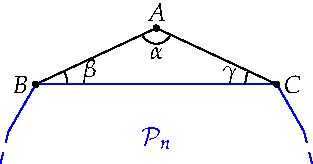
\includegraphics[width=\textwidth]{induction-05-polygon}\\
% 		Case 1: $A$ outside $\mathcal{P}_n$\\[25pt]
% 		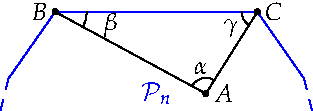
\includegraphics[width=\textwidth]{induction-06-polygon}\\
% 		Case 2: $A$ inside $\mathcal{P}_n$
% 	\end{minipage}\\[8pt]
% 	$\mathcal{P}_{n+1}$ again has interior angles summing to $180[(n+1)-2]$\textdegree.
% \end{proof}
% 
% \footnotetext{We are obscuring two subtleties here. It is a fact, though not an obvious one, that it is always possible to choose a vertex $A$ so that the new polygon $\cP_n$ doesn't cross itself. Read about `ears' and `mouths' of polygons and triangulation if you're interested. There are also two other, less likely, cases which we didn't consider: when deleting a point from an ($n+1$)-gon it is possible to obtain  an $(n-1)$-gon, or even an $(n-2)$-gon. To think it out, try drawing a 12-gon in the shape of a Star of David. Deleting one of the outer corners creates a 9-gon! Dealing with these cases strictly requires strong induction, so we return to them later.}

%Wellorder stuff!
%     \item Prove: $n! \le \left(\frac{n + 1}{2}\right)^n$.\par
%      (\emph{Hint: find a formula for the sum of the first $n$ positive integers})
%   


% \subsubsection*{Optional: Density of the Rationals}
% 
% In our last example, we offer a more direct application of $\N$ being well-ordered. One of the  key properties of the rational numbers $\Q$ is their density in the real line. Intuitively, the idea is that no matter how close you "zoom in" on the real line, you can always locate a rational number. We formalize this with the following definition.
% 
% \begin{defn}
% We say a set $A \subseteq \R$ is \textbf{dense} (in $\R$) if for any real numbers $x$ and $y$ such that $x < y$, there is  $a \in A$ such that $x < a < y$.
% \end{defn}
% 
% So if you take two real numbers, you can always find an element from $A$ in between them, no matter how close the two real numbers are from each other. Our goal will be to prove that the rational numbers $\Q$ are dense in $\R$. For this, we will use the well-orderedness of $\N$ along with the following:
% 
% \begin{axiom}
% The real numbers $\R$ have the \textbf{Archimedean property}, that is, for any real numbers $x,y > 0$, there is $n \in \N$ such that $nx > y$.
% \end{axiom}
% 
% It is not really necessary to take this as an axiom as the Archimedean property of $\R$ can be proved from more basic principles. However, this requires some knowledge about how to construct the real numbers which lies beyond the scope of this course. Back to our goal, we need the following lemma which states that if two real numbers differ by more than $1$, then there must be an integer between them.
% 
% \begin{lemm}\label{lemm:rationaldensityprep}
% Suppose we have $x,y \in \R$ with $y - x > 1$. Then there exists $k \in \Z$ such that $x < k < y$.
% \end{lemm}
% 
% \begin{proof}
% The idea is to take $k$ to be the least integer greater than $x$. We will show such an integer exists using the fact that $\N$ is well-ordered. Let $A = \{n \in \Z : n > x\}$. Then $A \neq \emptyset$ by the Archimedean property (why?). Let $m \in \Z$ be a number such that $m < x$ (this is another application of the Archimedean property), and thus $m < n$ for all $n \in A$, by definition of $A$. Let 
% \[
% S = \{n - m + 1 : n \in A\}.
% \]
% So $S \subseteq \N$ and since $A \neq \emptyset$, we have $S \neq \emptyset$. Since $\N$ is well-ordered, $S$ has  a minimum element $s$. Then $k = s + m - 1$ is the minimum element of $A$ (why?).
% 
% By definition $x < k$. But by minimality of $k$, $k - 1 \notin A$, i.e., $x \geq k - 1$. Thus $x < k \leq x + 1$. Finally, since $y - x > 1$, we have $x + 1 < y$. All together, $x < k \leq x + 1 < y$. So $k$ is as required.
% \end{proof}
% 
% Now we can prove our main result.
% 
% \begin{thm}
% The rational numbers $\Q$ are dense in $\R$.
% \end{thm}
% 
% \begin{proof}
% Let $x,y \in \R$ with $x < y$ be arbitrary. We need to find $r \in \Q$ with $x < r < y$. Then $y - x > 0$. By the Archimedean property, there is $n \in \N$ such that $n(y - x) > 1$. Since $ny - nx > 1$, we can apply Lemma \ref{lemm:rationaldensityprep} to get $k \in \Z$ such that $nx < k < ny$. As $n \geq 1 > 0$, dividing yields $x < \frac{k}{n} < y$. Take $r = \frac{k}{n} \in \Q$.
% \end{proof}


\clearpage



\subsection{Strong Induction}\label{sec:strongind}

The principle of mathematical induction (Theorem \ref{thm:ind}) is often known as \emph{weak} induction. The primary difference with \emph{strong} induction is that the induction step assumes more than one proposition.

\begin{thm}{Principle of Strong Induction}{indstrong}
	Let $l\ge m$ be fixed integers and suppose $P(n)$ is a proposition, one for each $n\in\Z_{\ge m}$. Suppose:
	\begin{quote}
		\begin{tabular}{@{}ll}
			\emph{Base case(s)}: &$P(m),P(m+1),\ldots,P(l)$ are true\\[5pt]
			\emph{Induction step}: &$\forall n\ge l,\ \bigl(P(m)\wedge P(m+1)\wedge\cdots\wedge P(n)\bigr)\Longrightarrow P(n+1)$
		\end{tabular}
	\end{quote}
	Then $P(n)$ is true for all $n\ge m$.
\end{thm}

Exercise \ref{exs:strongindproof} provides a proof by showing that strong and weak induction are equivalent. We instead concentrate on a few examples. The main additional challenge of strong induction lies in determining how many base cases are required and in identifying precisely how to phrase the induction hypothesis: in practice one rarely needs to use all the propositions $P(m),\ldots,P(n)$ explicitly.


\begin{example}{Fibonacci numbers}{fibonacci}
	This famous sequence $(f_n)_{n=1}^\infty=(1,1,2,3,5,8,13,21,\ldots)$ is defined by the 2\nd-order recurrence relation
	\[
		\begin{cases}
			f_{n+1}=f_n+f_{n-1}&\text{if }n\ge 2\\
			f_1=f_2=1&
		\end{cases}
	\]
	While the Fibonacci sequence seems to be increasing, it also appears to be less than doubling at each step, suggesting the claim
	\[
		\tcbhighmath{\forall n\in\N,\ f_n<2^n}
	\]
	We prove this using strong induction. \emph{Two base cases} are suggested since the sequence is defined by two initial conditions ($f_1=f_2=1$): in the language of the Theorem, $m=1$ and $l=2$. Moreover, the fact that each term from $f_3$ onwards is the sum of its \emph{two predecessors} suggests that the induction step requires the explicit use of two propositions.
	\begin{quote}
		\begin{proof}
			\begin{description}
				\item[\normalfont\emph{Base cases} ($n=1,2$):] $f_1=1<2^1$ and $f_2=1<2^2$.
				\item[\normalfont\emph{Induction step}:] Fix $n\ge 2$ and suppose\footnotemark{} that $f_{n-1}<2^{n-1}$ and $f_n<2^n$. Then
				\[
					f_{n+1}=f_n+f_{n-1}<2^n+2^{n-1}<2^n+2^n=2^{n+1}
				\]
			\end{description} 
			By induction, $f_n<2^n$ for all $n\in\N$.
		\end{proof}
	\end{quote}
	The Fibonacci numbers satisfy many identities which can often be established by induction (e.g., Exercises \ref{exs:fib} \& \ref{exs:fib2}).
\end{example}

\vspace{-5pt}

\footnotetext{To follow Theorem \ref{thm:indstrong} precisely, we would assume that $f_k<2^k$ for \emph{all} $k\le n$. Feel free to write this if you like, though our phrasing is more typical. Since we only make explicit use of two cases in the induction step, it is clearer to state these concretely rather than introducing a new variable $k$.}

\goodbreak

Before seeing further examples, it is instructive to consider why we really needed strong induction to prove our Fibonacci example. Here are two broken attempts to prove the claim by weak induction.

\begin{proof}[Broken Proof A]
	\begin{description}
		\item[\normalfont\emph{Base case} ($n=1$):] $f_1=1<2^1$.
		\item[\normalfont\emph{Induction step}:] Fix $n\ge 2$ and suppose that $f_n<2^n$. Then\footnotemark
		\[
			f_{n+1}=f_n+f_{n-1}<2^n+\text{????} \tag*{\phantom{\qedhere}}
		\]
	\end{description} 
\end{proof}

\footnotetext{The induction step requires $n\ge 2$ so as to invoke the recurrence relation: $f_{n+1}=f_n+f_{n-1}$ is meaningless when $n=1$ ($f_{n-1}=f_0$ doesn't exist).}
	
What is the problem? The induction hypothesis assumes $f_n<2^n$, but not anything about $f_{n-1}$: we are stuck! Let's correct this flaw by making the induction hypothesis as in the correct proof.

\begin{proof}[Broken Proof B]
	\begin{description}
		\item[\normalfont\emph{Base case} ($n=1$):] $f_1=1<2^1$.
		\item[\normalfont\emph{Induction step}:] Fix $n\ge 2$ and suppose that $f_{n-1}<2^{n-1}$ and $f_n<2^n$. Then
		\[
			f_{n+1}=f_n+f_{n-1}<2^n+2^{n-1}<2^n+2^n=2^{n+1}
		\]
	\end{description} 
	By induction, $f_n<2^n$ for all $n\in\N$.\phantom{\qedhere}
\end{proof}

Where is the problem now? Consider the first instance, $n=2$, in which the induction step is invoked:
\[
	f_3=\textcolor{red}{f_2}+f_1<\textcolor{red}{2^2}+2^1
\] 
We haven't proved enough base cases to get us started: the single base case establishes $f_1<2^1$, but not $\textcolor{red}{f_2<2^2}$. The induction step correctly establishes the chain of implications
\[
	P(1)\wedge P(2)\Longrightarrow P(3),\quad P(3)\wedge P(4)\Longrightarrow P(5),\quad P(4)\wedge P(5)\Longrightarrow P(6),\ \ldots
\]
but we can only get the process started if we prove \emph{both} base cases $P(1)$ \emph{and} $\textcolor{red}{P(2)}$.\smallbreak

The moral here is to try the induction step as scratch work. Your attempt should tell you \emph{if} you need strong induction and \emph{how many} base cases are required.


\begin{example}{}{}
	A sequence of integers $(a_n)_{n=0}^\infty$ is defined by
	\[
		\begin{cases}
			a_{n+1}=5a_n-6a_{n-1}&\text{if }n\ge 1\\
			a_0=0,\ a_1=1
		\end{cases}
	\]
	We prove by induction that $a_n=3^n-2^n$ for all $n\in\N_0$.
	
	\begin{quote}
		\begin{proof}
			\begin{description}
				\item[\normalfont\emph{Base cases} ($n=0,1$):] $a_0=0=3^0-2^0$ and $a_1=1=3^1-2^1$.
				\item[\normalfont\emph{Induction step}:] Fix $n\ge 1$ and suppose that$a_k=3^k-2^k$ for all $k\le n$. Then
				\begin{align*}
					a_{n+1}&=5a_n-6a_{n-1}=5(3^n-2^n)-6(3^{n-1}-2^{n-1})\\
					&=(15-6)3^{n-1}+(10-6)2^{n-1}=3^{n+1}-2^{n+1}
				\end{align*}
			\end{description} 
			By induction, $a_n=3^n-2^n$ for all $n\in\N_0$.
		\end{proof}
	\end{quote}
\end{example}

\goodbreak


For another sequential induction example in the same vein, see Exercise \ref{ex:ind3} where \emph{three} base cases are required, and the induction step explicitly uses \emph{three} propositions.\medbreak

To see strong induction in all its glory, where the induction step requires \emph{all} previous propositions, we prove the existence part of the Fundamental Theorem of Arithmetic, which states that all integers $\ge 2$ can be (uniquely) expressed as a product of primes: e.g.,\ $3564=2^2\times 3^4\times 11$. 


\begin{thm}{}{fundarith}
	Every integer $n\ge 2$ is either prime or a product of primes.
\end{thm}

This provides the missing piece in our discussion of Euclid's Theorem (\ref{thm:euclidprime}) on the existence of infinitely many primes. First recall Definition \ref{defn:irreducible}: $p\in\N_{\ge 2}$ is \emph{prime} if and only if its only positive divisors are itself and 1. A non-prime $q\in\N_{\ge 2}$ is said to be \emph{composite}: $\exists a,b\in\N_{\ge 2}$ such that $q=ab$.


\begin{proof}
	We prove by induction.
	\begin{description}
		\item[\normalfont\emph{Base case} ($n=2$):] The only positive divisors of 2 are itself and 1, hence 2 is prime.
		\item[\normalfont\emph{Induction step}:] Fix $n\ge 2$ and suppose that \emph{every} natural number $k$ satisfying $2\le k\le n$ is either prime or a product of primes. There are two possibilities:
		\begin{itemize}
		  \item $n+1$ is prime. Certainly $n+1$ is divisible by a prime!
		  \item $n+1$ is composite. Then $n+1=ab$ for some natural numbers $a,b\ge 2$. Clearly $a,b\le n$; by the induction hypothesis, \emph{both} are prime or the product of primes. Therefore $n+1$ is also the product of primes.
		\end{itemize}
	\end{description}
	By induction we see that all natural numbers $n\ge 2$ are either prime, or a product of primes.
\end{proof}

Think carefully about why \emph{only one} base case is required!


\begin{exercises}{}{}
	A reading quiz and several questions with linked video solutions can be found \href{http://www.math.uci.edu/~ndonalds/math13/selftest/5-3-strongind.html}{online}.

	\begin{enumerate}  
  	\item Define sequence $(b_n)_{n=1}^\infty$ as follows:
  	\[
  		\begin{cases}
				b_{n+1}=2b_n+b_{n-1} &\text{if } n\ge 2\\
				b_1=3, \ b_2=6
			\end{cases}
		\]
		Prove by induction that $b_n$ is divisible by 3 for all $n\in\N$.
	
	
		\item\label{ex:ind3strong} Define a sequence $(c_n)_{n=0}^\infty$:
	 	\[
	 		\begin{cases}
				c_{n+1}=\frac{49}8c_n-\frac{225}8c_{n-2}&\text{if }n\ge 2\\
				c_0=0, \ c_1=2, \ c_2=16
			\end{cases}
		\]
		Prove by induction (use three base cases!) that $c_n=5^n-3^n$ for all $n\in\N_0$.
		
		
		\item\label{exs:fib} Let $f_n$ be the $n\th$ Fibonacci number (Example \ref{ex:fibonacci}). Prove the following by induction $\forall n\in\N$:
		\begin{enumerate}
		  \item $\sum\limits_{k=1}^nf_k^2=f_nf_{n+1}$ \qquad\qquad (b)\lstsp $f_n\ge\left(\frac 32\right)^{n-2}$
		\end{enumerate}
		(\emph{Hints: Weak induction is good enough for (a); why?})
	
	
		\goodbreak
		

	  \item\label{exs:fib2} Extending Exercise \ref{exs:fib}(b), prove \emph{Binet's formula} for the $n\th$ Fibonacci number:
	  \[
	  	f_n=\frac 1{\sqrt 5}\bigl(\phi^n-\hat\phi^n\bigr) \quad \text{where}\quad \phi=\frac 12(1+\sqrt{5})\text{ and } \hat\phi=\frac 12(1-\sqrt{5})
	  \]
		(\emph{$\phi$ is the famous \emph{golden ratio}: $\phi,\hat\phi$ are the solutions to the quadratic equation $x^2=x+1$})
  		
		
		\item Prove by induction that every $n\in\N$ can be written in the form
	  \[
	    n=2^{r_1}+2^{r_2}+\cdots+2^{r_\ell}
	  \]
	  for some $\ell\in\N$ and \emph{distinct} integers $r_1,r_2,\ldots r_\ell \ge 0$.\par
	  (\emph{Hints: try proving in the style of Theorem \ref{thm:fundarith}; consider the cases when $n+1$ is even/odd separately})
	
	
		\item\label{exs:strongindproof} Prove the principle of strong induction (Theorem \ref{thm:indstrong}) by applying \emph{weak induction} to a new family of propositions $Q(n)$ via:
		\[
			Q(n)\iff P(m)\wedge P(m+1)\wedge\cdots\wedge P(n)
		\]
	
	
		\item Consider the proof of Theorem \ref{thm:fundarith}.
		\begin{enumerate}
	  	\item If the Theorem is written in the form $\forall n\in\N_{\ge 2}, P(n)$, what is the proposition $P(n)$?
	  	\item Explicitly carry out the induction step for the three situations $n+1=9$, $n+1=106$ and $n+1=45$. How many different ways can you perform the calculation for $n+1=45$? 
	  	\item Explain why it is only necessary in the induction step to assume that all integers $k$ satisfying $2\le k\le\frac{n+1}2$ are prime or products of primes.
		\end{enumerate}

		\item\label{exs:primedef2} In this question we use the alternative definition of prime (Exercise \ref*{sec:gcd}.\ref{exs:primedef1}).\footnotemark
		\begin{quote}
			An integer $p\ge 2$ is \emph{prime} if and only if $\forall a,b\in\N,\ p\mid ab\implies p\mid a$ or $p\mid b$.
		\end{quote}
		Let $p$ be prime, let $n\in\N$, and let $\lst an$ be natural numbers such that $p\mid a_1a_2\cdots a_n$. Prove by induction that,
		\[
			p\mid a_i\ \text{ for some }\ i\in\{1,2,\ldots,n\}
		\]
	  (\emph{Hint: $n=1$ isn't really part of the induction, but you can treat it as a base case})
	  
	    
	  \item The \emph{Fundamental Theorem of Arithmetic} states that every integer $n\ge 2$ can be written as a product of prime factors in a \emph{unique} way (up to reordering of the prime factors). In other words, 
		\begin{itemize}
	    \item[i.] $n=p_1p_2\cdots p_k$ for some primes $p_1,p_2,\ldots,p_k$, \ and,
	    \item[ii.] If $n=q_1q_2\cdots q_\ell$ for primes $q_1,q_2,\ldots,q_\ell$, then $k=\ell$ and $p_i=q_i$ after possibly reordering the prime factors. 
		\end{itemize}
	  Part i.{} is Theorem \ref{thm:fundarith}. Using Exercise \ref{exs:primedef2}, or otherwise, supply a proof of part ii.
		
	\end{enumerate}
\end{exercises}

\footnotetext{This is the strict definition of \emph{prime,} while Definition \ref{defn:irreducible} is the  definition of \emph{irreducible.} For the integers, Exercise \ref*{sec:gcd}.\ref{exs:primedef1} says that these concepts are synonymous.}


%\graphicspath{{notes/6setsii/}}

\section{Set Theory, Part II}

In this chapter we return to set theory and consider several more-advanced constructions.

\subsection{Cartesian Products}

You have been working with Cartesian products for years, referring to a point in the plane $\R^2$ by its \emph{Cartesian co-ordinates} $(x,y)$. The basic idea is that each of the co-ordinates $x$ and $y$ is a member of the set $\R$. The same approach can be used for any two sets.

\begin{defn}
Let $A$ and $B$ be sets. The \emph{Cartesian product} of $A$ and $B$ is the set
\[A\times B=\{(a,b):a\in A\text{ and }b\in B\}.\]
\end{defn}

\noindent $A\times B$ is simply the set of \emph{ordered pairs} $(a,b)$ where $a\in A$ and $b\in B$.

\begin{examples}
	\item The Cartesian product of the real line $\R$ with itself is the $xy$-plane: rather than writing $\R\times\R$ which is unwieldy, we write $\R^2$.
	\[\R^2=\R\times\R=\{(x,y):x,y\in\R\}.\]
	More generally, $\R^n=\underbrace{\R\times\R\times\cdots\R}_{\text{$n$ times}}$ is the set of $n$-tuples of real numbers:
	\[\R^n=\{(x_1,x_2,\ldots,x_n):x_1,x_2,\ldots,x_n\in\R\}.\]
	\item If $A=\{1,2,3\}$ and $B=\{\alpha,\beta\}$, then the Cartesian product of $A$ and $B$ is
	\[A\times B=\{(1,\alpha),\ (1,\beta),\ (2,\alpha),\ (2,\beta),\ (3,\alpha),\ (3,\beta)\}\]
	Notice that this is a \emph{different set} to the Cartesian product of $B$ and $A$:
	\[B\times A=\{(\alpha,1),\ (\beta,1),\ (\alpha,2),\ (\beta,2),\ (\alpha,3),\ (\beta,3)\}\]
	\item Suppose you go to a restaurant where you have a choice of one main course and one side. The menu might be summarized set-theoretically: consider the sets
	\begin{gather*}
	\text{Mains}=\{\text{fish, steak, eggplant, pasta}\}\\
	\text{Sides}=\{\text{asparagus, salad, potatoes}\}
	\end{gather*}
	The Cartesian product Mains\,$\times$\,Sides is the set of all possible meals made up of one main and one side. It should be obvious that there are $4\times 3=12$ possible meal choices.
\end{examples}

\noindent These last two examples illustrates the next theorem, which explains the use of the word \emph{product.}

\begin{thm}
If $A$ and $B$ are finite sets, then $\nm{A\times B}=\nm A\cdot\nm B$.
\end{thm}

\begin{proof}
Label the elements of each set and list the elements of $A\times B$ lexicographically. If $\nm A=m$ and $\nm B=n$, then we have:
\[\begin{array}{rccccccl}
A\times B=\big\{&(a_1,b_1),&(a_1,b_2),&(a_1,b_3),&\cdots&(a_1,b_n),&\\
&(a_2,b_1),&(a_2,b_2),&(a_2,b_3),&\cdots&(a_2,b_n),&\\
&\vdots&\vdots&\vdots&&\vdots&\\
&(a_m,b_1),&(a_m,b_2),&(a_m,b_3),&\cdots&(a_m,b_n)&\big\}
\end{array}\]
It should be clear that every element of $A\times B$ is listed exactly once. There are $m$ rows and $n$ columns, thus $\nm{A\times B}=mn$.
\end{proof}

Before we go any further, consider the complement of a Cartesian product $A\times B$. If you had to guess an expression for $\comp{(A\times B)}$, you might well try $\comp A\times\comp B$. Let us think more carefully.
% \begin{align*}
% (x,y)\in\comp{(A\times B)}&\iff (x,y)\not\in A\times B&&(x,y)\in\comp A\times\comp B\iff x\not\in A\text{ and }x\not\in B\\
% &\iff \neg((x,y)\in A\times B)&&\\
% &\iff \neg(x\in A\text{ and }y\in B)&&\\
% &\iff x\not\in A\text{ or }y\not\in B&&
% \end{align*}
\begin{gather*}
\begin{aligned}
(x,y)\in\comp{(A\times B)}&\iff (x,y)\not\in A\times B\\
&\iff \neg((x,y)\in A\times B)\\
&\iff \neg(x\in A\text{ and }y\in B)\\
&\iff x\not\in A\text{ or }y\not\in B
\end{aligned}
\end{gather*}
However $(x,y)\in\comp A\times\comp B\iff x\not\in A\text{ and }x\not\in B$. Since the definition of Cartesian product involves \emph{and,} its negation, by De Morgan's laws, involves \emph{or.} It follows that the complement of a Cartesian product is \emph{not a Cartesian product!} For more on this, see Exercise \hyperref[ex:cartneg]{\thesubsection.\ref*{ex:cartneg}}.\\


As an example of a basic set relationship involving Cartesian products, we prove a theorem.

\begin{thm}\label{thm:cartex}
Let $A,B,C,D$ be any sets. Then $(A\times B)\cup(C\times D)\subseteq(A\cup C)\times(B\cup D)$.
\end{thm}

\begin{proof}
Since we are dealing with Cartesian products, the general element has the form $(x,y)$.\\
\noindent\begin{minipage}{0.65\textwidth}
Let $(x,y)\in(A\times B)\cup(C\times D)$. Then 
\[(x,y)\in A\times B\qquad \text{or}\qquad (x,y)\in C\times D.\]
But then
\[(x\in A\text{ and }y\in B)\qquad\text{or}\qquad(x\in C\text{ and }y\in D).\]
Clearly $x\in A$ or $x\in C$, so $x\in A\cup C$.\\
Similarly $y\in B$ or $y\in D$, so $y\in B\cup D$.\\
Therefore $(x,y)\in (A\cup C)\times(B\cup D)$, as required.
\end{minipage}
\qquad
\begin{minipage}{0.28\textwidth}
\centering
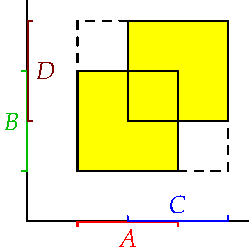
\includegraphics[width=\textwidth]{setsii-04-cartesian}
\end{minipage}
\end{proof}

\noindent The picture is an visualization of the theorem, where we assume that the sets $A,B,C$ and $D$ are all intervals of real numbers. $(A\times B)\cup(C\times D)$ is the yellow shaded region, while $(A\cup C)\times(B\cup D)$ is the larger dashed square. While helpful, the picture is not a proof! The theorem is a statement about \emph{any} sets, whereas the picture implicitly assumes that these sets are intervals.\\
For an application of the picture, it should be clear that if $x\in C\setminus A$ and $y\in B\setminus D$, then $(x,y)\in (A\cup C)\times (B\cup D)$ but $(x,y)\not\in (A\times B)\cup(C\times D)$. We do not therefore expect these sets to be equal.

\paragraph{Self-test Questions}

	\begin{enumerate}
    \item The Cartesian product of sets $A$ and $B$ is \underline{\phantom{the set of ordered pairs $\{(a,b):a\in A,\ b\in B\}$,\qquad}}
    \item True or false: $A\times B=\emptyset\iff A=B=\emptyset$.
    \item True or false: The cardinality of $A\times B$ is at least as large as $\max(\nm A,\nm B)$.
  \end{enumerate}

\subsection*{Exercises}

\begin{enumerate}\renewcommand{\labelenumi}{\thesubsection.\theenumi}
  \item\begin{enumerate}
    \item Suppose that $A=\{1,2\}$ and $B=\{3,4,5\}$. State the set $A\times B$ in roster notation.
    \item Sketch both $A\times B$ and $B\times A$ using dots on the plane. What do you observe about your pictures?
    \item If $A,B,C$ are any sets, we may define the triple Cartesian product as
    \[A\times B\times C=\big\{(a,b,c):a\in A,\ b\in B,\ c\in C\big\}\]
    If $C=\{6,7\}$ and $A,B$ are as above, state the set $A\times B\times C$ in roster notation.
  \end{enumerate}
  
  \item Consider the following subintervals of the real line: $A=[2,5],\ B=(0,4)$.
  \begin{enumerate}
    \item Express the set $\comp{(A\setminus B)}$ in interval notation, as a disjoint union of intervals.
    \item Draw a picture of the set $\comp{(A\setminus B)}\times (B\setminus A)$.
  \end{enumerate}

	\item Rewrite the condition
	\[(x,y)\in (\comp{A}\cup B)\times (C\setminus D)\]
	in terms of (some of) the following propositions:
	\[x\in A,\quad x\not\in A,\quad x\in B,\quad x\not\in B,\quad y\in C,\quad y\not\in C,\quad y\in D,\quad y\not\in D.\]

	\item Let $A=[1,3]$, $B=[2,4]$ and $C=[2,3]$. \emph{Prove or disprove} that
	\[(A\times B)\cap (B\times A)=C\times C.\]
	\emph{Hint: Draw the sets $A\times B$, $B\times A$ and $C\times C$ in the Cartesian plane. The picture will give you a hint on whether or not the statement is true, but it does not constitute a proof.}
	
	\item A straight line subset of the plane $\R^2$ is a subset of the form
	  \[A_{a,b,c}=\{(x,y):ax+by=c\},\quad\text{for some constants $a,b,c$, with $ab\neq 0$.}\]
	  \begin{enumerate}
	  \item Draw the set $A_{1,2,3}$. Is it a Cartesian product?
	 	\item Which straight line subsets in the plane $\R^2$ are Cartesian products? Otherwise said, find a condition on the constants $a,b,c$ for which the set $A_{a,b,c}$ is a Cartesian product.
		\end{enumerate}
	
	\item\label{ex:cartneg} Draw a picture, similar to that in Theorem \ref{thm:cartex}, which illustrates the fact that
	\[\comp{(A\times B)}\neq \comp A\times \comp B.\]
	Using your picture, write the set $\comp{(A\times B)}$ in the form
	\[(C_1\times D_1)\cup (C_2\times D_2)\cup\cdots\]
	where each of the unions are \emph{disjoint:} that is $i\neq j\implies (C_i\times D_i)\cap (C_j\times D_j)=\emptyset$. You don't have to prove your assertion.
		
	\item Prove that $A\cap B=\emptyset\iff (A\times B)\cap(B\times A)=\emptyset$.
	
  \item\begin{enumerate}
		\item Suppose that $\nm A=3$, and $\nm B=4$. What are the minimum and maximum values for the cardinalities $\nm{(A\times B)\cap(B\times A)}$ and $\nm{(A\times B)\cup(B\times A)}$?
		\item More generally, suppose that $\nm A=m$, $\nm B=n$ and $\nm{A\cap B}=c$. What are the above cardinalities?
	\end{enumerate}
	
  \item Prove the following by induction. For all $n\in\N$, if $A_1,\ldots,A_n$ are finite sets, then
  \[\nm{A_1\times\cdots\times A_n}=\nm{A_1}\cdots\nm{A_n}\] 
	
	\item Let $E\subseteq\N\times\N$ be the smallest subset which satisfies the following conditions:
	\begin{itemize}
		\item Base case: $(1,1)\in E$
		\item Generating Rule I: If $(a,b)\in E$ then $(a,a+b)\in E$
		\item Generating Rule II: If $(a,b)\in E$ then $(b,a)\in E$
	\end{itemize}

	\begin{enumerate}
		\item Show in detail that $(4,3)\in E$.
		\item Show by induction that for every $n\in\N$, $(1,n)\in E$.
		\item (Very hard!!!) Show that $E=\{(a,b)\in\N\times\N:\gcd(a,b)=1\}$. \emph{Think carefully about how the Euclidean algorithm works, and what the generating rules might have to do with it\ldots}
	\end{enumerate}
	
	\item A strict set-theoretic definition requires you to build the ordered pair $(a,b)$ as a set: typically $(a,b)=\{a,\{a,b\}\}$. One then proves that $(a,b)=(c,d)\iff a=c$ and $b=d$.
	\begin{enumerate}
	  \item One of the axioms of set theory (\emph{regularity}) says that there is no set $a$ for which $a\in a$. Use this to prove that the cardinality of $(a,b)=\{a,\{a,b\}\}$ is two.
	  \item Prove that $(a,b)=(c,d)\implies\begin{cases}
	  a=c\text{ and }b=d,\\
	  \qquad\quad\text{\emph{or}}\\
	  a=\{c,d\}\text{ and }c=\{a,b\}.
	  \end{cases}$
	  \item In the second case, prove that there exists a set $S$ such that $a\in S\in a$. The axiom of regularity also says that this is illegal. Conclude that $(a,b)=(c,d)\iff a=c$ and $b=d$.
	\end{enumerate}
\end{enumerate}
\newpage

\subsection{Power Sets}

Thusfar we have seen how to build new sets from old using the operations of subset, complement, union, intersection and Cartesian product. There is essentially only one further method whereby we can produce new sets; given a set $A$, we consider the collection of all of the subsets of $A$ and we insist that this collection is a set.

\begin{defn}
The \emph{power set} of $A$ is the set $\cP(A)$ of all subsets of $A$. That is,
\[\cP(A)=\{B:B\subseteq A\}.\]
Otherwise said: $B\in\cP(A)\iff B\subseteq A$.
\end{defn}

\begin{examples}
	\item Let $A=\{1,3,7\}$. Then $A$ has the following subsets, listed by how many elements are in each subset.
\[\begin{array}{ll}
\text{0-elements:}&\emptyset\\
\text{1-element:}&\{1\},\ \{3\},\ \{7\}\\
\text{2-elements:}&\{1,3\},\ \{1,7\},\ \{3,7\}\\
\text{3-elements:}&\{1,3,7\}
\end{array}\]
Gathering these together, we have the power set:
\[\cP(A)=\Bigl\{\emptyset,\{1\},\{3\},\{7\},\{1,3\},\{1,7\},\{3,7\},\{1,3,7\}\Bigr\}.\]
\item Consider $B=\Bigl\{1,\bigl\{\{2\},3\bigr\}\Bigr\}$. It is essential that you use different size set brackets to prevent confusion. $B$ has only \emph{two} elements, namely $1$ and $\bigl\{\{2\},3\bigr\}$. We can gather the subsets of $B$ in a table.
\[\begin{array}{ll}
\text{0-elements:}&\emptyset\\
\text{1-element:}&\{1\},\ \Bigl\{\bigl\{\{2\},3\bigr\}\Bigr\}\\
\text{2-elements:}&\Bigl\{1,\bigl\{\{2\},3\bigr\}\Bigr\}
\end{array}\]
In the second line, remember that to make a subset out of a single element you must surround the element with set brackets. Thus $1\in B\implies \{1\}\subseteq B$ and
\[\bigl\{\{2\},3\bigr\}\in B\implies \Bigl\{\bigl\{\{2\},3\bigr\}\Bigr\}\subseteq B.\]
The power set of $B$ is therefore
\[\cP(B)=\biggl\{\emptyset,\ \{1\},\ \Bigl\{\bigl\{\{2\},3\bigr\}\Bigr\},\ \Bigl\{1,\bigl\{\{2\},3\bigr\}\Bigr\}\biggr\}.\]
\end{examples}\pagebreak[2]


\paragraph{Notation}

Be absolutely certain that you understand the difference between $\in$ and $\subseteq$. It is easy to become confused when considering power sets. In the context of the previous examples, here are eight propositions. Which are true and which are false?\footnote{Only (a), (d), and (g) are true. Make sure you understand why!}
\[\begin{array}{r@{\quad}l@{\qquad\qquad}r@{\quad}l@{\qquad\qquad}r@{\quad}l@{\qquad\qquad}r@{\quad}l}
\text{(a)}&1\in A
		&\text{(b)}&1\in\cP(A)
		&\text{(c)}&\{1\}\in A
		&\text{(d)}&\{1\}\in\cP(A)\\
\text{(e)}&1\subseteq A
		&\text{(f)}&1\subseteq\cP(A)
		&\text{(g)}&\{1\}\subseteq A
		&\text{(h)}&\{1\}\subseteq\cP(A)
\end{array}\]

\noindent As a further exercise in being careful with notation, consider the following theorem.

\begin{thm}\label{thm:powersub}
If $A\subseteq B$, then $\cP(A)\subseteq\cP(B)$.
\end{thm}

\begin{proof}
Suppose that $A\subseteq B$ and let $C\in\cP(A)$. We must show that $C\in\cP(B)$.\\
By definition, $C\in\cP(A)\implies C\subseteq A$. Since subset inclusion is transitive (Theorem \hyperlink{thm:subsettranslnk}{\ref*{thm:subsettrans}}), we have
\[C\subseteq A\subseteq B\implies C\subseteq B.\]
This says that $C\in\cP(B)$. Therefore $\cP(A)\subseteq\cP(B)$.
\end{proof}

\noindent It is very easy to get confused by the proof of this theorem. Exercises \hyperref[ex:powersub1]{\thesubsection.\ref*{ex:powersub1}} and \hyperref[ex:powersub2]{\thesubsection.\ref*{ex:powersub2}} discuss things further.


\subsubsection*{Cardinality and Power Sets}

Let's investigate how the cardinality of a set and its power set are related. Consider a few basic examples where we list all of the subsets, grouped by cardinality.
\[\begin{array}{|c||c|c|c|c||c|}
\hline
\text{Set }A&\text{0-elements}&\text{1-element}&\text{2-elements}&\text{3-elements}&\nm{\cP(A)}\\\hline
\emptyset&\emptyset&&&&1\\\hline
\{a\}&\emptyset&\{a\}&&&1+1=2\\\hline
\{a,b\}&\emptyset&\{a\},\{b\}&\{a,b\}&&1+2+1=4\\\hline
\{a,b,c\}&\emptyset&\{a\},\{b\},\{c\}&\{a,b\},\{a,c\},\{b,c\}&\{a,b,c\}&1+3+3+1=8\\\hline
\end{array}\]
You should have seen this pattern before: we are looking at the first few lines of Pascal's Triangle.\footnote{If you know a little about combinations from probability, it should be clear that a set $A$ with $n$ elements has precisely ${}^nC_r=\binom nr=\frac{n!}{r!(n-r)!}$ distinct $r$-element subsets.} It should be no surprise that if $\nm A=4$, then $\nm{\cP(A)}=1+4+6+4+1=16$. The progression $1,2,4,8,16,\ldots$ in the final column immediately suggests the following theorem.

\begin{thm}\label{thm:powercard}
Suppose that $A$ is a finite set. Then $\nm{\cP(A)}=2^{\nm A}$.
\end{thm}

\noindent Conjuring up a proof may seem daunting given how little we know about $A$! In fact we have only one thing to work with: the \emph{cardinality} of $A$. Indeed you might find it helpful to rephrase the theorem as follows:
\[\forall n\in\N_0,\ \ \nm A=n\implies \nm{\cP(A)}=2^{n}\]
Viewed this way, we see that we want to prove an infinite collection of propositions, indexed by the set $\N_0$:  induction seems like the way forward. What might the induction step look like? The basic idea is that every set with $n+1$ elements is the disjoint union of a set with $n$ elements and a single-element set. The induction step is essentially the observation that any $n+1$-element set $B$ has \emph{twice} the number of subsets of some $n$-element set $A$. It is instructive to see an example of this before writing the proof. 

\begin{example}
Let $B=\{1,2,3\}$. Now choose the element $3\in B$ and delete it to create the smaller set
\[A=\{1,2\}=B\setminus\{3\}.\]
We can split the subsets of $B$ into two groups: those which contain 3 and those which do not. In the following table we list all of the subsets of $B$. In the first column are those subsets $X$ which do not contain 3. These are exactly the subsets of $A$. In the second column are the subsets $Y=X\cup\{3\}$ of $B$ which do contain 3.
\[\begin{array}{c|c}
X&X\cup\{3\}\\\hline
\emptyset&\{3\}\\
\{1\}&\{1,3\}\\
\{2\}&\{2,3\}\\
\{1,2\}&\{1,2,3\}
\end{array}\]
It is clear that $B$ has twice the number of subsets of $A$.
\end{example}

\noindent This method of pairing is exactly mirrored in the proof.

\begin{proof}
We prove by induction on the cardinality of $A$. For each $n\in\N_0$, we consider the proposition
\[\nm A=n\implies\nm{\cP(A)}=2^n.\tag*{($\ast$)}\]
(\emph{Base Case})\quad If $n=0$, then $A=\emptyset$ (Theorem \hyperlink{thm:subsettranslnk}{\ref*{thm:subsettrans}}). But then $\cP(A)=\{\emptyset\}$, whence $\nm{\cP(A)}=1=2^0$.\\
(\emph{Induction Step})\quad Fix $n\in\N_0$ and assume that ($\ast$) is true for this $n$. That is, we assume that any set with $n$ elements has $2^n$ subsets. Now let $B$ be \emph{any} set with $n+1$ elements. Choose one of the elements $b\in B$ and define $A=B\setminus\{b\}$. The subsets of $B$ can then be separated into the following two types:
\begin{enumerate}\itemsep0pt
  \item Subsets $X\subseteq B$ which do not contain $b$.
  \item Subsets $Y\subseteq B$ which contain $b$.
\end{enumerate}
In the first case, $X$ is really a subset of $A$.\\
In the second case we can write $Y=X\cup\{b\}$, where $X$ is again a subset of $A$.\\
Each subset $X\subseteq A$ therefore corresponds to precisely two subsets $X$ and $X\cup\{b\}$ of $B$. Since $\nm{A}=n$, the induction hypothesis tells us that there are $2^n$ subsets $X\subseteq A$, whence
\[\nm{\cP(B)}=2\nm{\cP(A)}=2^{n+1}.\]
By induction, $(\ast)$ is true for all $n\in\N_0$.
\end{proof}

\noindent Once you understand the proof, you should compare it to the proof of Theorem \ref{thm:polygon} on the interior angles of a polygon: the idea is very similar. Exercise \hyperref[ex:binom]{\thesubsection.\ref*{ex:binom}} gives an alternative proof of this result.\\

\noindent As a final example, we consider the interaction of power sets and Cartesian products.

\begin{example}
Suppose that $A=\{a\}$ and $B=\{b,c\}$. Then
\[A\times B=\{(a,b),(a,c)\}.\]
The power set $\cP(A\times B)$ therefore contains $2^2=4$ elements: indeed
\[\cP(A\times B)=\Big\{\emptyset,\ \{(a,b)\},\ \{(a,c)\},\ \{(a,b),(a,c)\}\Big\}.\]
The power sets of $A$ and $B$ have 2 and 4 elements respectively:
\[\cP(A)=\big\{\emptyset,\{a\}\big\},\qquad\cP(B)=\big\{\emptyset,\{b\},\{c\},\{b,c\}\big\}.\]
The Cartesian product of the power sets therefore has $2\times 4=8$ elements:
\begin{multline*}
\cP(A)\times\cP(B)
=\Big\{\big(\emptyset,\emptyset\big),\  \big(\emptyset,\{b\}\big),\  \big(\emptyset,\{c\}\big),\  \big(\emptyset,\{b,c\}\big),\\*
\big(\{a\},\emptyset\big),\  \big(\{a\},\{b\}\big),\  \big(\{a\},\{c\}\big),\  \big(\{a\},\{b,c\}\big)\Big\}.
\end{multline*}
It should be clear from this example not only that $\cP(A\times B)\neq\cP(A)\times\cP(B)$, but that the elements of the two sets are completely different. The elements of $\cP(A\times B)$ are \emph{sets of ordered pairs,} while the elements of $\cP(A)\times\cP(B)$ are \emph{ordered pairs of sets.}
\end{example}



\paragraph{Self-test Questions}

	\begin{enumerate}
    \item The power set of a set $A$ is \underline{\phantom{the set of all subsets of $A$\qquad\qquad\qquad}}
    \item Which of the following are correct statements?
    \[[0,1)\in\cP(\R),\qquad 7\in\cP(\N),\qquad \{(3,5),(2,9)\}\subseteq\cP(\N\times\N),\qquad \{4,\pi\}\in\cP(\R)\]
  \end{enumerate}


\subsection*{Exercises}

\begin{enumerate}\renewcommand{\labelenumi}{\thesubsection.\theenumi}
  \item Find $\cP(A)$ and $\nm{\cP(A)}$ for the following:\\[5pt]
	\begin{tabular}{r@{\ \ }l@{\qquad\qquad\qquad\qquad}r@{\ \ }l}
	(a)&$A=\{1,2\}$.&(d)&$A=\{\emptyset,1,\{a\}\}$.\\[2pt]
	(b)&$A=\{1,2,3\}$.&(e)&$A=\Big\{\big\{1,2\big\},3,\big\{4,\{5\}\big\}\Big\}$.\\[5pt]
	(c)&$A=\bigl\{(1,2),(2,3)\bigr\}$.&(f)&$A=\Big\{(1,2),\ 3,\ \bigl(4,\{5\}\bigr)\Big\}$.
	\end{tabular}
	
	\item Let $A=\{1,3\}$ and $B=\{2,4\}$.
	\begin{enumerate}
	  \item Draw a picture of the set $A\times B$.
	  \item Compute $\cP(A\times B)$.
	  \item What is the cardinality of $\cP(A)\times\cP(B)$? \emph{Don't compute the set!}
	\end{enumerate}
  
	\item Determine whether the following statements are true or false (\emph{in (b), the symbol $\subsetneq$ means `proper subset'}). Justify your answers.
  \begin{enumerate}
    \item If $\{7\}\in\cP(A)$, then $7\in A$ and $\{7\}\notin A$.
    \item Suppose that $A,B$ and $C$ are sets such that $A\subsetneq\cP(B)\subsetneq C$ and $\nm A=2$. Then $\nm C$ can be 5, but $\nm C$ cannot be 4.
    \item If a set $B$ has one more element than a set $A$, then $\cP(B)$ has at least two more elements than $\cP(A)$.
    \item Suppose that the sets $A,B,C$ and $D$ are all subsets of $\{1,2,3\}$ with cardinality two. Then at least two of these sets are equal. 
  \end{enumerate}
  
	\item\label{ex:powersub1} Here are three incorrect proofs of Theorem \ref{thm:powersub}. Explain why each fails.
	\begin{enumerate}
		\item Let $x\in\cP(A)$. Then $x\in A$. Since $A\subseteq B$, we have $x\in B$. Therefore $x\in\cP(B)$, and so $\cP(A)\subseteq\cP(B)$.
		\item Let $A=\{1,2\}$ and $B=\{1,2,3\}$. Then $\cP(A)=\{\emptyset,\{1\},\{2\},A\}$, and\\
		$\cP(B)=\{\emptyset,\{1\},\{2\},\{3\},\{1,2\},\{1,3\},\{2,3\},B\}$. Thus $\cP(A)\subseteq\cP(B)$.
		\item Let $x\in A$. Since $A\subseteq B$, we have $x\in B$. Since $x\in A$ and $x\in B$, we have $\{x\}\in\cP(A)$, and $\{x\}\in\cP(B)$.
	\end{enumerate}
	
	\item\label{ex:powersub2} Consider the converse of Theorem \ref{thm:powersub}. Is it true or false? Prove or disprove your conjecture.
	
	\item\begin{enumerate}
	  \item Prove that $\cP(A)\cup\cP(B)\subseteq\cP(A\cup B)$. Provide a counter-example to show that we do not expect equality.
	  \item Does anything change if you replace $\cup$ with $\cap$ in part (a)? Justify your answer.
	\end{enumerate}
	
	\item Consider the proof of Theorem \ref{thm:powercard}. Let $B$ be a set with $n+1$ elements, let $b\in B$ and let $A=B\setminus\{b\}$. Prove that the function $f:\cP(A)\times\{1,2\}\to\cP(B)$ defined by
	\[f(X,1)=X,\qquad f(X,2)=X\cup\{b\}\]
	is a bijection, and that consequently, by Theorem \ref{thm:finitecard}, $\nm{\cP(A)\times\{1,2\}}=\nm{\cP(B)}$.
	
	\item\label{ex:binom} We use the following notation for the binomial coefficient: $\binom nr=\frac{n!}{r!(n-r)!}$. This symbol denotes the number of distinct ways one can choose $r$ objects from a set of $n$ objects.
	\begin{enumerate}
	  \item Use the definition of the binomial coefficient to prove the following:
	  \[\text{If } 1\le r\le n,\ \text{ then }\ \binom{n+1}r=\binom nr+\binom n{r-1}.\]
		\item Prove by induction that $\forall n\in\N_0,\,\sum\limits_{r=0}^n\binom nr=2^n$.\\
		\emph{Hint: Use part (a) in the induction step. Note that the smallest $n$ for which it applies is $n=1\ldots$}
		\item Explain why part (b) provides an alternative proof of Theorem \ref{thm:powercard}.
	\end{enumerate}
	\emph{If you found this easy, try proving the binomial theorem: $\forall n\in\N,\,(x+y)^n=\sum\limits_{r=0}^n\binom nrx^ry^{n-r}$.}
\end{enumerate}
\newpage

\subsection{Indexed Collections of Sets}

In this section we consider collections of sets $A_n$, where each $n$ lies in some \emph{indexing set} $I$. It is often the case that $I=\N$ or $\Z$. If $I$ is some other set, for example the real numbers $\R$, the label for the index may be chosen accordingly: e.g. $A_x$.

% \begin{examples}
% 	\item Let $A_n=[-n,n]\subseteq \R$, for each $n\in\N$. For example $A_1=[-1,1]$, $A_2=[-2,2]$, etc.
% 	\item Let $A_n=(n,n+1]\subseteq\R$, for each $n\in\Z$. E.g.\ $A_{-17}=(-17,-16]$.
% 	\item Let $A_n=[0,\frac 1n)\subseteq\R$, for each $n\in\N$. E.g.\ $A_{1000}=[0,\frac 1{1000})$.
% 	\item Let $A_n=(0,\frac 1n)\subseteq\R$, for each $n\in\N$.
% 	\item Let $A_n=\{x\in\R:\nm{x^2-1}<\frac 1n\}$, for each $n\in\N$. Here $A_3=\Big(-\sqrt{\frac 43},-\sqrt{\frac 23}\Big)\cup \Big(\sqrt{\frac 23},\sqrt{\frac 43}\Big)$.
% \end{examples}

\begin{defn}\label{defn:indexed}
Given a family of indexed sets $\{A_n:n\in I\}$, we may form the \emph{union} and \emph{intersection} of the collection:
\begin{gather*}
\bigcup_{n\in I}A_n=\{x:x\in A_n\text{\emph{ for some} }n\in I\},\\
\bigcap_{n\in I}A_n=\{x:x\in A_n\text{\emph{ for all} }n\in I\}.
\end{gather*}
Otherwise said,
\begin{gather*}
x\in\bigcup_{n\in I}A_n\iff \exists n\in I\text{ such that }x\in A_n\\
x\in\bigcap_{n\in I}A_n\iff \forall n\in I\text{ we have }x\in A_n
\end{gather*}
A indexed collection $\{A_n:n\in I\}$ is \emph{pairwise disjoint} if $A_m\cap A_n=\emptyset$ whenever $m\neq n$.
\end{defn}

\noindent When the indexing set is $\N$, it is common to use the notations $\bigcup\limits_{n=1}^\infty A_n$ and $\bigcap\limits_{n=1}^\infty A_n$.

\begin{example}
Let the indexing set be $I=\{\alpha,\beta,\gamma\}$, and let
\[A_\alpha=\{1,3,5\},\qquad A_\beta=\{2,3,4,6\},\qquad A_\gamma=\{1,2,3,6\}.\]
It should be clear that
\[\bigcup_{i\in I}A_i=A_\alpha\cup A_\beta\cup A_\gamma=\{1,2,3,4,5,6\}\]
and
\[\bigcap_{i\in I}A_i=A_\alpha\cap A_\beta\cap A_\gamma=\{3\}\]
\end{example}

\noindent The following Theorem is almost immediate given the definitions of union and intersection: can you supply a formal proof?

\begin{thm}
Let $\{A_n:n\in I\}$ be an indexed collection of sets, and let $m\in I$. Then
\[A_m\subseteq\bigcup_{n\in I}A_n\quad\text{and}\quad \bigcap_{n\in I}A_n\subseteq A_m.\]
\end{thm}



% \begin{proof}
% \begin{enumerate}
% 	\item Let $x\in A_m$. Then $\exists i\in I$ such that $x\in A_i$, and hence $x\in\bigcup\limits_{i\in I}A_i$.
% 	\item Let $x\in\bigcap\limits_{i\in I}A_i$. Then $\forall i\in I$ we have $x\in A_i$. In particular, $x\in A_j$.\qedhere
% \end{enumerate}
% \end{proof}


\subsubsection*{Infinite Unions and Intersections: don't take limits!}

The challenge with indexed sets often involves computing unions and intersections of \emph{infinitely many} sets. Be very careful with this: it is very tempting to `take limits' when this doesn't make sense. With this in mind, we dissect an important example.\\

\noindent For each $n\in\N$, consider the interval $A_n=\Bigl[0\,,\,\frac 1n\Bigr)$. We analyze the collection $\{A_n:n\in\N\}$. First observe that $m\le n\implies \frac 1n\le \frac 1m\implies A_n\subseteq A_m$; the sets are therefore nested:
\[A_1\supseteq A_2\supseteq A_3\supseteq A_4\supseteq\cdots\tag*{($\ast$)}\]
Since every set in the collection is a subset of $A_1$, it follows that this is the union,
\[\bigcup_{n=1}^\infty A_n=A_1=[0,1).\]
Before considering the full intersection, we first compute all finite intersections. Since the sets $A_n$ are nested in the form ($\ast$), it follows that any \emph{finite} intersection is simply the smallest of the listed sets: i.e., for any constant $m\in\N$ we have
\[\bigcap_{n=1}^mA_n=A_m=\Bigl[0\,,\,\frac 1m\Bigr).\]
Observe that this is non-empty \emph{for every $m$}. Now what about the infinite intersection? You might be tempted to take a limit and make an argument such as
\[\bigcap\limits_{n=1}^\infty A_n\overset{?}{=}\lim_{m\to\infty}\bigcap_{n=1}^mA_n\overset{?}{=}\lim_{m\to\infty}\Bigl[0\,,\,\frac 1m\Bigr)\overset{?}{=}\Bigl[0\,,\lim_{m\to\infty}\frac 1m\Bigr)=[0,0).\]
Quite apart from the issue that $[0,0)$ is ugly and could only mean the empty set, we should worry about whether this is a legitimate use of limits. It isn't! We are only allows to take limits of sequences of numbers, not of \emph{sets.} Perhaps you could forgive the abuse of limits if the approach yielded the correct conclusion. Unfortunately it doesn't: the infinite intersection is in fact non-empty, and we claim the following.

\begin{thm}
$\bigcap\limits_{n=1}^\infty A_n=\{0\}$.
\end{thm}

\noindent Before we give a formal proof, it is instructive to see a calculation. Let us show, for example, that $\frac 29\not\in\bigcap\limits_{n=1}^\infty A_n$. To prove that $\frac 29$ is not in the intersection of \emph{all} the $A_n$, it is enough to exhibit a single integer $m$ such that $\frac 29\not\in A_m$. The picture shows that we can choose $m=10$: since $\frac 1{10}<\frac 29$, we have $\frac 29\not\in [0,\frac 1{10}]=A_{10}$. Since $\frac 29\not\in A_{10}$, we conclude that $\frac 29\not\in\bigcap\limits_{n=1}^\infty A_n$.
\begin{center}
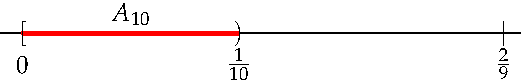
\includegraphics[width=0.5\textwidth]{setsii-06-intervalex}
\end{center}

\begin{proof}
We prove that $x\in\bigcap\limits_{n=1}^\infty A_n\iff x=0$.\\
Suppose that $x\in\bigcap\limits_{n=1}^\infty A_n$. Then $x\in\bigl[0\,,\,\frac 1n\bigr)$ for all $n$. Otherwise said,
\[\forall n\in\N,\text{ we have }0\le x<\frac 1n.\tag*{($\dag$)}\]
Certainly $x=0$ satisfies these inequalities.\\
Now suppose, for a contradiction, that $x>0$. Since $\lim\limits_{n\to\infty}\frac 1n=0$, we can certainly choose\footnote{Explicitly, you may choose choose $N=\lceil\frac 1x\rceil$, or anything larger. Here $\lceil x\rceil$ is the \emph{ceiling function:} the smallest integer greater than or equal to $x$.} $N$ large enough so that $\frac 1N\le x$. But this says that $x\not\in A_N$, which contradicts ($\dag$).\\
The intersection contains no positive elements, and we conclude that
\[\bigcap\limits_{n=1}^\infty A_n=\{0\}.\tag*{\qedhere}\]
\end{proof}

\noindent By modifying the sets $A_n$ to either include or exclude endpoints, we can obtain slightly different results. Consider each of the following in turn. How would the argument for computing each intersection differ from what we did above?
\begin{itemize}
  \item If $B_n=\Bigl(0\,,\,\frac 1n\Bigr)$, then $\bigcap\limits_{n=1}^\infty B_n=\emptyset$.
  \item If $C_n=\Bigl(0\,,\,\frac 1n\Bigr]$, then $\bigcap\limits_{n=1}^\infty C_n=\emptyset$.
  \item If $D_n=\Bigl[0\,,\,\frac 1n\Bigr]$, then $\bigcap\limits_{n=1}^\infty D_n=\{0\}$.
\end{itemize}
The moral of these examples is that you cannot naïvely apply limits to sequences of sets. Your intuition is often a good guide, but that doesn't mean you should trust it blindly!\\

Here are a few more examples.

 
\begin{examples}
	\item\label{ex:index2} Let $A_n=[n,n+1)\subseteq\R$, for each $n\in\Z$. For example,
\[A_3=[3,4),\quad\text{and}\quad A_{-17}=[-17,-16).\]
In this case the sets $A_n$ are pairwise disjoint, and we have
\[\bigcup\limits_{n\in\Z}A_n=\R,\quad\text{and}\quad\bigcap\limits_{n\in\Z}A_n=\emptyset.\]
To prove the former, note that $\forall x\in\R$ we have $x\in[n,n+1)$ where $n=\lfloor x\rfloor$ is the greatest integer which is less than or equal to $x$: i.e. $x\in A_{\lfloor x\rfloor}$.


	\item\vspace*{5pt} For each $n\in\N$, let $A_n=[-n,n]$. Each of the sets $A_n$ is a closed interval. E.g.,
	\[A_1=[-1,1],\qquad A_2=[-2,2],\qquad A_3=[-3,3].\]
	It should be clear that $n\le m\implies A_n\subseteq A_m$ so that we have a \emph{nested} sequence of sets:
	\[A_1\subseteq A_2\subseteq A_3\subseteq\cdots\]
	It follows immediately that the intersection is $\bigcap\limits_{n\in\N}A_n=A_1=[-1,1]$.\\
	With a little thinking you might hypothesize that the union is $\bigcup\limits_{n\in\N}A_n=\R$. To prove this, assume that $x\in\R$ is non-zero, and observe that
	\[-\lceil\nm x\rceil\le x\le\lceil\nm x\rceil\implies x\in A_{\lceil\nm x\rceil}\]
	Since $0\in A_1$, it follows that $\R\subseteq\bigcup\limits_{n\in\N}A_n$, whence these sets are equal.\\
	If the notation is causing difficulty, consider for example,
	\[-3.124\in A_{\lceil 3.124\rceil}=A_4.\]
	
	\item For each $n\in\N$, let $A_n=\{x\in\R:\nm{x^2-1}<\frac 1n\}$. Before computing the union and intersection of these sets, it is helpful to write each set as a pair of intervals. Note that
	\[\nm{x^2-1}<\frac 1n\iff -\frac 1n< x^2-1<\frac 1n\iff \sqrt{1-\frac 1n}< \nm x< \sqrt{1+\frac 1n}.\]
	Therefore
	\[A_n=\left(-\sqrt{1+\tfrac 1n},-\sqrt{1-\tfrac 1n}\right)\cup\left(\sqrt{1-\tfrac 1n},\sqrt{1+\tfrac 1n}\right).\]
	As the picture suggests, the sets $A_n$ are nested: $A_1\supseteq A_2\supseteq A_3\supseteq A_4\supseteq\cdots$.\\[5pt]
	\noindent\begin{minipage}{0.5\textwidth}
	Since $A_1$ is the largest of the nested sets, we see that
	\[\bigcup\limits_{n\in\N}A_n=A_1=(-\sqrt{2},0)\cup(0,\sqrt{2}).\]
	For the intersection, note that
	\begin{align*}
	\forall n\in\N,\ x\in A_n&\iff \forall n\in\N,\ \nm{x^2-1}<\frac 1n\\
	&\iff x^2-1=0.
	\end{align*}
	It follows that $\bigcap\limits_{n\in\N}A_n=\{1,-1\}$.
	\end{minipage}\hfill\begin{minipage}{0.38\textwidth}
	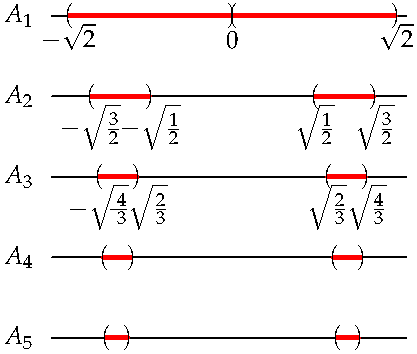
\includegraphics[width=\textwidth]{setsii-05-intervalex}
	\end{minipage}
\end{examples}


\subsubsection*{Indexed Unions: Don't Confuse Sets and Elements}

It is easy to confuse and important to distinguish between the sets
\[\{A_n:n\in I\}\qquad\text{and}\qquad\bigcup_{n\in I}A_n.\]
The first is a set whose \emph{elements} are themselves sets. The second is the collection of all elements in \emph{any} set $A_n$. Consider the following examples.


\begin{examples}
	\item For each $n\in\{1,2,3\}$, let $A_n$ be the plane $\{(x,y,z):x+ny+n^2z=1\}\subseteq\R^3$.\\[2pt]
	The indexed collection $\{A_1,A_2,A_3\}$ has \emph{three} elements: each of the planes $A_1,A_2,A_3$ is an element in its own right.\\
  The union $A_1\cup A_2\cup A_3$ is an \emph{infinite} set consisting of all the \emph{points} lying on any of the three planes.\\
  For the intersection, a little work with simultaneous equations should convince you that
  \[(x,y,z)\in\negthickspace\negthickspace\bigcap_{n\in\{1,2,3\}}\negthickspace\negthickspace A_n\iff
  \begin{cases}
  x+y+z=1\\
  x+2y+4z=1\\
  x+3y+9z=1
  \end{cases}\iff (x,y,z)=(1,0,0).\]
  Thus $\bigcap A_n=\{(1,0,0)\}$. The planes are drawn below.
  
  \item\label{ex:projline} Let $I=\R\cup\{\infty\}$. For each $m\in I$, let $A_m$ be the line\footnote{We include the vertical line $A_\infty$.} through the origin in $\R^2$ with gradient $m$.\\[2pt]
  Each element of $\{A_m:m\in I\}$ is a \emph{line}: there is one for each direction through the origin.\\
  The union $\bigcup A_m$ consists of all of the \emph{points} that lie on \emph{any} line through the origin. Since any point in the plane lies on some line through the origin, we see that $\bigcup A_m=\R^2$.\\
  It should be clear that all the lines intersect at the origin, and so $\bigcap A_m=\{(0,0)\}$.\\
  The collection of lines $\{A_m:m\in I\}$ is the famous \emph{projective space} $\mathbb P(\R^2)$; this is a very different set from $\R^2$!\\
  This example also shows that indexing sets don't have to be simple sets of integers. It is also possible to index the same set using $I=[0,\pi)$. If we define $B_\theta$ to be the line through the origin making an angle $\theta$ with the positive $x$-axis, we would then have $B_\theta=A_{\tan\theta}$.
\end{examples}

\begin{center}
\begin{minipage}[b]{0.45\textwidth}
\centering
\includemedia[width=0.8\textwidth, transparent=false, activate=onclick, add3Djscript=asylabels.js, add3Djscript=3Dspintool.js, 3Dmenu,
3Dcoo=-0.2646917402744293 -9.039887428283691 17.85630226135254,
3Dc2c=0.781423807144165 -0.5375411510467529 0.31690123677253723,
3Droo=261.5486749519297,
3Dlights=Headlamp]{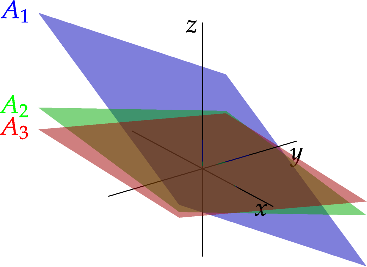
\includegraphics{setsii-01-planes+0_0}}{setsii-01-planes+0.prc}\\[15pt]
Example 1: Three elements, or an infinite number?
\end{minipage}\qquad\qquad
\begin{minipage}[b]{0.35\textwidth}
\centering
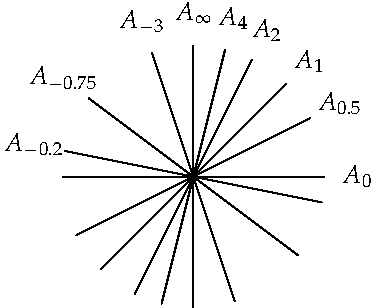
\includegraphics[width=\textwidth]{setsii-03-projective}\\
Example 2: Elements in $\mathbb P(\R^2)$
\end{minipage}
\end{center}


\subsubsection*{Finite Decimals}\label{ex:finitedec}

Here is another example where our intuition of `taking the limit' leads us astray. This time it is the union that behaves surprisingly.\\

\noindent For each $n\in\N$, let $A_n$ be the set of decimals of length $n$. That is
\[A_n=\bigl\{0.a_1a_2\ldots a_n:\text{where each $a_i\in\{0,1,\ldots,9\}$}\bigr\}.\]
For example $0.134\in A_3$. Since $0.134=0.1340$, we also have $0.134\in A_4$. Once again we have a nested sequence of sets
\[A_1\subseteq A_2\subseteq A_3\subseteq A_4\subseteq\cdots\]
The infinite intersection is therefore simply
\[\bigcap_{n\in\N}A_n=A_1=\{0,0.1,\ldots,0.9\}.\]
Now consider a finite union: if $m\in\N$, then
\[\bigcup_{n=1}^mA_n=A_m=\bigl\{x\in [0,1):x\text{ has a decimal representation of length $\le m$}\bigr\}.\]
At this point, we might be inclined to take the limit as $m\to\infty$ of the \emph{property} `length $m$ decimal.' If so, then it would seem that the infinite union should be the entire\footnote{We would include $1=0.9999\cdots$} interval $[0,1]$.\\
What is wrong with our reasoning? We have again abused the idea of limits: one cannot take the limit of a property! Instead we use the definition:
\begin{align*}
x\in\bigcup_{n\in\N}A_n&\iff\exists n\in\N\text{ such that }x\in A_n\\
&\iff\exists n\in\N \text{ such that $x$ is a decimal of length $n$.}
\end{align*}
It follows that
\[\bigcup_{n\in\N}A_n=\big\{x\in[0,1):x\text{ has a \emph{finite} decimal representation}\big\}\]
In particular, there are no irrational numbers in $\bigcup\limits_{n\in\N}A_n$:
\[\text{If $x\in A_n$, then $y=10^nx$ is an integer, whence $x=\frac y{10^n}\in\Q$.}\]
Many rational numbers are also excluded. For example $\frac 13=0.3333\cdots$ is not in any set $A_n$ and is therefore not in the union.


\subsubsection*{The Cantor Set}\label{ex:cantor}

We finish this section with a bit of fun. We can use infinite intersections to create self-similar sets, otherwise known as \emph{fractals.} The \emph{Cantor middle-third set} is a famous example.\\

\noindent Staring with the interval $C_0=[0,1]$, we construct a sequence of sets $C_n$ for each $n\in\N_0$ by repeatedly removing the middle third of each of the intervals contained in $C_n$.

\begin{minipage}{0.40\textwidth}
$C_0=[0,1]$,\\[4pt]
$C_1=[0,\frac 13]\cup [\frac 23,1]$,\\[4pt]
$C_2=[0,\frac 19]\cup [\frac 29,\frac 13]\cup [\frac 23,\frac 79]\cup [\frac 89,1]$, etc.
\end{minipage}
\begin{minipage}{0.55\textwidth}
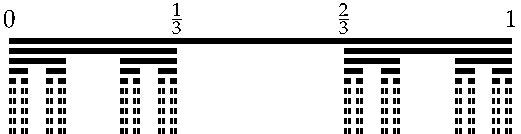
\includegraphics[width=\textwidth]{setsii-02-cantor}
\end{minipage}\\

\noindent The sequence is drawn up to $C_{9}$, with an animation below. To see the detail for the last few sets, try zooming in as far as you can.\vspace{-5pt}
\begin{center}
\animategraphics[width=\textwidth]{1}{setsii-07-cantor}{0}{9}
\end{center}\vspace{-8pt}

\begin{defn}
The \emph{Cantor set} $\mathcal C$ is the infinite intersection $\mathcal C=\negthickspace\bigcap\limits_{n=0}^\infty\negthickspace C_n$.
\end{defn}

\noindent This set has several interesting properties.\\

\noindent{\bf Zero Measure} (length)\quad Intuitively, the \emph{length} of a set of real numbers is the sum of the lengths of all the intervals contained in the set. Since we start with the interval $[0,1]$ and remove a third of the set each time, it should be clear that
\[\operatorname{length}(C_0)=1,\qquad \operatorname{length}(C_1)=\frac 23,\qquad\operatorname{length}(C_2)=\left(\frac 23\right)^2,\quad\text{etc.}\]
Induction then gives us
\[\operatorname{length}(C_n)=\left(\frac 23\right)^n.\]
As $n\to\infty$ this goes to zero, so the Cantor set contains no intervals. This at least seems reasonable from the picture.\\

\noindent{\bf Infinite Cardinality}\quad The Cantor set $\mathcal{C}$ contains the endpoints of every interval removed at any stage of its construction. In particular, $\frac 1{3^n}\in\mathcal C$ for all $n\in\N_0$, and so $\mathcal C$ is an \emph{infinite} set. Indeed it is more than merely infinite, it is \emph{uncountably} so, as we shall see in Chapter \ref{sec:card}.\\

\noindent{\bf Self-similarity}\quad If $\frac 13\mathcal C$ means `take all the elements of $\mathcal C$ and divide them by three,' and $\frac 13\mathcal C+\frac 23$ means `take all the elements of $\frac 13\mathcal C$ and add $\frac 23$,' then
\[\mathcal C=\frac{\mathcal C}{3}\cup\left(\frac{\mathcal C}{3}+\frac 23\right).\tag*{($\ast$)}\]
Otherwise said, $\mathcal C$ is made up of two shrunken copies of itself, a classic property of fractals. If you were to zoom into the Cantor set far enough that you couldn't see the whole set, you would not know what the scale was. In the following animation we are repeatedly zooming in on the second (of four) groups of points.
\begin{center} 
\animategraphics[width=0.6\textwidth,loop]{6}{setsii-08-cantor}{0}{22}
\end{center}

\subsubsection*{Optional: Analyzing the Cantor Set}

To get further with the Cantor set, it is necessary to explicitly describe the elements of the set. This can be accomplished using the \emph{ternary representation.}\label{page:cantor} It can be shown that every number $x\in[0,1]$ may be written in the form\footnote{Analogous to a decimal representation $x=\sum\limits_{n=1}^\infty 10^{-n}a_n=\frac{a_1}{10}+\frac{a_2}{10^2}+\frac{a_3}{10^3}+\cdots$ where $a_n\in\{0,1,2,\ldots,9\}$.}
  \[x=\sum\limits_{n=1}^\infty 3^{-n}a_n=\frac{a_1}{3}+\frac{a_2}{3^2}+\frac{a_3}{3^3}+\cdots\]
  where each $a_n\in\{0,1,2\}$. We write $x=[0.a_1a_2a_3\cdots]_3$. For example:
\[[0.12]_3=\frac 13+\frac 2{3^2}=\frac 59,\qquad \frac{64}{243}=\frac 2{3^2}+\frac 1{3^3}+\frac 1{3^5}=[0.02101]_3,\qquad 1=[0.22222\cdots]_3.\]
For this last, use the formula for the sum of a geometric series to calculate $\sum\limits_{n=1}^\infty 2\left(\frac 13\right)^n=2\cdot\frac{1/3}{1-1/3}=1$.\\
To convince yourself of the existence of a ternary representation, note that if $0\le x<1$ it follows that $x<3$ and so, we can take
\[a_1=\lfloor 3x\rfloor\in\{0,1,2\}\]
Now repeat, with $a_2=\lfloor x-\frac{a_1}3\rfloor$, etc.
  It can also be shown that the only possibility whereby $x$ can have two ternary expansions is if one of them terminates. The other will eventually become a sequence of repeating 2's. For example:\footnote{This is ticklish to prove, as is the corresponding result for decimals: compare with $1=0.99999999\cdots$}
  \[[0.0222222\cdots]_3=[0.1]_3=\frac 13\quad \text{and}\quad [0.10122222\cdots]_3=[0.102]_3=\frac 13+\frac 2{27}=\frac{11}{27}.\]
  We can now describe precisely the elements of each of the sets $C_n$ and consequently the Cantor set.

\begin{thm}
$C_n$ is the set of all numbers $x\in[0,1]$ with a ternary expansion whose first $n$ digits are only 0 or 2. It follows that $\mathcal C$ is the set of $x\in[0,1]$ with a ternary expansion containing only 0 and 2.
\end{thm}

\noindent The Theorem tells us that the Cantor set contains \emph{a lot} of elements. For example:
\[[0.020202020\cdots]_3=2\sum_{n=1}^\infty 3^{-2n}=\frac{2/9}{1-1/9}=\frac 14\]
is an element of the Cantor set! What is strange is that $\frac 14$ is not the endpoint of any of the open intervals deleted during the construction of $\mathcal C$, and yet we've already established that $\mathcal C$ contains no intervals! Cantor introduced his set precisely because it was so challenging to the traditional concept of size: $\mathcal C$ seems to simultaneously have very few elements and enormously many.

\begin{proof}
We prove by induction.\\[2pt]
(\emph{Base Case})\quad The proposition is clearly true for $C_0=[0,1]$, as there is nothing to check.\\[2pt]
(\emph{Induction Step})\quad Assume that the proposition is true for some fixed $n\in\N_0$. Analogously to ($\ast$) above, observe that $C_{n+1}$ is built from two shrunken copies of $C_n$:
\[C_{n+1}=\frac 13C_n\cup\left(\frac 13C_n+\frac 23\right).\]
Now consider what division by 3 and addition of $\frac 23$ does to a ternary representation.
\begin{itemize}
  \item Since $\frac 13\sum_{n=1}^\infty 3^{-n}a_n=\sum_{n=1}^\infty 3^{-n-1}a_1$, we see that multiplication by $\frac 13$ shifts a ternary representation one position to the right.\footnote{Compare to multiplication of a decimal by $\frac 1{10}$.}
	\[\frac 13[0.a_1a_2a_3\ldots]_3=[0.0a_1a_2a_3\ldots]_3\]
	\item Since $\frac 23=[0.2]_3$ we see that
	\[\frac 23+\frac 13[0.a_1a_2a_3\ldots]_3=[0.2a_1a_2a_3\ldots]_3\]
\end{itemize}
By the induction hypothesis, $C_n$ contains only 0's and 2's in its first $n$ entries. By moving ternary representations one step to the right and inserting 0 or 2 in the first position, we conclude that $C_{n+1}$ contains only 0's and 2's in its first $n+1$ entries.\\[2pt]
By induction the proposition is true for all $n\in\N_0$.
\end{proof}

\noindent Other fractal sets based on $\mathcal C$ include the Cantor dust $\mathcal C\times\mathcal C$, the \href{http://en.wikipedia.org/wiki/Sierpinski_carpet}{Sierpi\'nski carpet} and \href{http://en.wikipedia.org/wiki/Sierpinski_triangle}{gasket}, and the \href{http://en.wikipedia.org/wiki/Koch_snowflake}{von Koch snowflake.}



\paragraph{Self-test Questions}

	\begin{enumerate}
    \item If $\{A_n:n\in I\}$ is a collection of sets then
    \begin{enumerate}
      \item $x\in \bigcap_{n\in I}A_n\iff$ \underline{\phantom{$\exists n\in I:x\in A_n$,\qquad}}
      \item $x\in \bigcup_{n\in I}A_n\iff$ \underline{\phantom{$\forall n\in I:x\in A_n$,\qquad}}
  \end{enumerate}
    \item For any real number $x$, the \emph{ceiling} function applied to $x$ is the value $\lceil x\rceil$, which is defined to be \underline{\phantom{the least integer greater than or equal to $x$\qquad}}
    \item What does it mean for a collection of sets $\{A_n:n\in\N\}$ to be \emph{nested?}
    \item True or false:
    \begin{gather*}
    B\subseteq \bigcup_{n\in I}A_n\iff \forall n\in I,\ B\subseteq A_n
    \end{gather*}
  \end{enumerate}

\subsection*{Exercises}

\begin{enumerate}\renewcommand{\labelenumi}{\thesubsection.\theenumi}
  	\item For each integer $n$, consider the set $B_n=\{n\}\times\R$.
	\begin{enumerate}
		\item Draw a picture of $\bigcup\limits_{n=2}^4B_n$ (in the Cartesian plane).\\
		\emph{Hint}:  $\bigcup \limits_{n=2}^{4} B_n= B_2 \cup B_3 \cup B_4.$
		\item Draw a picture of the set $C=[1,5]\times\{-2,2\}.$
		\emph{Careful!} $[1,5]$ is an interval, while $\{-2,2\}$ is a set containing two points.
		\item Compute $\left(\bigcup\limits_{n=2}^4B_n\right)\cap C$.
		\item Compute $\bigcup\limits_{n=2}^4\left(B_n\cap C\right)$.
		\item Compare $\left(\bigcup\limits_{n=2}^4B_n\right)\cap C$ and $\bigcup\limits_{n=2}^4\left(B_n\cap C\right)$. What do you notice?
	\end{enumerate}

  \item For each real number $r$, define the interval $S_r=[r-1,r+3]$. Let $I=\{1,3,4\}$. Determine $\bigcup\limits_{r\in I}S_r$ and $\bigcap\limits_{r\in I}S_r$.


  \item Give an example of four different subsets $A,B,C$ and $D$ of $\{1,2,3,4\}$ such that all intersections of two subsets are different.

  \item For each of the following collections of intervals, define an interval $A_n$ for each $n\in\N$ such that indexed collection $\{A_n\}_{n\in\N}$ is the given collection of sets. Then find both the union and intersection of the indexed collections of sets.
   \begin{enumerate}
     \item $\big\{[1,2+1),\,[1,2+\frac 12),\,[1,2+\frac 13),\,\ldots\big\}$
     \item $\big\{(-1,2),\,(-\frac 32,4),\,(-\frac 53,6),\,(-\frac 74,8),\,\ldots\big\}$
     \item $\big\{(\frac 14,1),\,(\frac 18,\frac 12),\,(\frac 1{16},\frac 14),\,(\frac 1{32},\frac 18), \,(\frac 1{64},\frac 1{16}),\,\ldots\big\}$
   \end{enumerate}
  
  \item For each non-negative real number $r\ge 0$ let 
  \[A_r=\big\{(x,y)\in\R^2:x^2+y^2=r^2\big\}\]
		\begin{enumerate}
  		\item Describe each of the sets $A_r$ geometrically.
  		\item Prove that $\bigcup_{r\in\R^+_0}A_r=\R^2$.
		\end{enumerate}

  \item For each real number $x$, let $A_x=\{3,-2\}\cup\{y\in\R:y>x\}$. Find $\bigcup\limits_{x\in\R}A_x$ and $\bigcap\limits_{x\in\R}A_x$.
  
  \item Use Definition \ref{defn:indexed} to prove the following results about nested sets.
		\begin{enumerate}
  		\item $A_1\supseteq A_2\supseteq A_3\supseteq\cdots\implies \bigcup\limits_{n\in\N}A_n=A_1$.
  		\item $A_1\subseteq A_2\subseteq A_3\subseteq\cdots\implies \bigcap\limits_{n\in\N}A_n=A_1$.
		\end{enumerate}

  \item Let $C_0(\R)$ denote the set of continuous functions $f:\R\to\R$ which satisfy $f(0)=0$.\\
  Let $A_f=\{x\in[0,1]:f(x)=0\}$ (so, for example, if $f:\R\to\R,\,x \mapsto x(2x-1)$, then $A_f=\{0,\frac 12\}$).
    \emph{Prove} that
  \[\bigcup\limits_{f\in C_0(\R)}\negthickspace\negthickspace A_f=[0,1]\qquad\text{and}\qquad\bigcap\limits_{f\in C_0(\R)}\negthickspace\negthickspace A_f=\{0\}.\]
		
	\item Let $A_n$ be the set of decimals of length $n$, as described on page \pageref{ex:finitedec}.
		\begin{enumerate}
	  	\item Prove directly that the cardinality of $A_n$ is $10^n$.
	  	\item Prove by induction that $\nm{A_n}=10^n$.
	  	\item Prove that $\bigcup\limits_{n=1}^\infty A_n\subseteq\Q$.
			\item Prove by contradiction that $\frac 13\not\in\bigcup\limits_{n=1}^\infty A_n$.
		\end{enumerate}

  \item Suppose that the following are true:
  \begin{itemize}
    \item $\forall n\in\N$, $A_n\neq\emptyset$.
    \item $m\ge n\Longrightarrow A_m\subseteq A_n$.
  \end{itemize}
  Prove or disprove the following conjectures:\\
	\begin{minipage}{0.4\textwidth}
  \begin{enumerate}
    \item $\bigcup\limits_{n=1}^{293}A_n\neq\emptyset$
    \item $\bigcap\limits_{n=1}^{293}A_n\neq\emptyset$
	\end{enumerate}
	\end{minipage}
	\begin{minipage}{0.4\textwidth}
  \begin{enumerate}\setcounter{enumii}{2}
    \item $\bigcup\limits_{n\in\N}^{\phantom{293}}A_n\neq\emptyset$
		\item $\bigcap\limits_{n\in\N}^{\phantom{293}}A_n\neq\emptyset$
	\end{enumerate}
	\end{minipage}

	\item (Hard) Let $A_n=\{\frac mn\in\Q:0<m<n, m\in \N\}$, for each $n\in\N$.
	\begin{enumerate}
		\item Write down $A_1,A_2,A_3,A_4$ explicitly.
		\item Prove that $A_m\subseteq A_{pm}$ for any $p\in\N$.
		\item Argue that $\bigcup\limits_{n\in\N}A_n=\Q\cap (0,1)$.
		\item Argue that further $\bigcup\limits_{n\in\N}A_{2n}=\Q\cap (0,1)$.
		\item Extend your proof to show that, for any fixed $p\in\N$, $\bigcup\limits_{n\in\N}A_{pn}=\Q\cap (0,1)$.
	\end{enumerate}
	
	\item In this question we construct a fractal shape, similar to the von Koch curve. Let $F_0=[0,1]$ be a straight line of length 1. Delete the segment between $\frac 12$ and $\frac 34$ to obtain the set
    \[F_1=[0,\tfrac 12]\cup[\tfrac 34,1]\]
    Now repeat: delete the third quarter of each of the two line segments in $F_1$ to obtain
    \[F_2=[0,\tfrac 14]\cup[\tfrac 38,\tfrac 12]\cup[\tfrac 34,\tfrac 78]\cup[\tfrac{15}{16},1]\]
    Suppose we repeat this process to create an infinite sequence of sets $F_0,F_1,F_2,F_3,F_4,\ldots$
  \begin{enumerate}
    \item Prove that the total length of all of the line segments making up the set $F_n$ is $\left(\frac 34\right)^n$.
    \item Prove by contradiction that the intersection $\bigcap\limits_{n=1}^\infty F_n$ does not contain any intervals of positive length.
    \item Now suppose that instead of simply deleting the third quarter of each line segment at each step, we replace it with the other three sides of a square. The first three steps in this process are shown below.
    \begin{center}
    \begin{tabular}{ccc}
    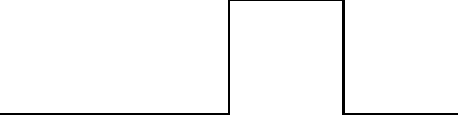
\includegraphics[width=0.27\textwidth]{fractal1}
    &
    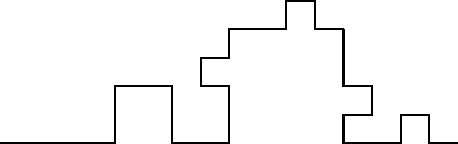
\includegraphics[width=0.27\textwidth]{fractal2}
    &
    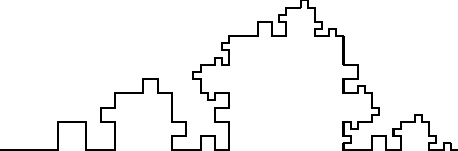
\includegraphics[width=0.27\textwidth]{fractal3}
   	\\
   	Step 1&Step 2&Step 3
    \end{tabular}
    \end{center}
    After each step, we are left with a curve. After step 1 the curve has length $\ell_1=\frac 32$. After step 2 the length is $\ell_2=\frac 94$. What is the \emph{length} $\ell_n$ of the curve after $n$ steps? Prove your assertion.
    \item Below is the result of repeating the steps in part 3 infinitely many times. What is the `length' of the resulting fractal curve?
    \begin{center}
    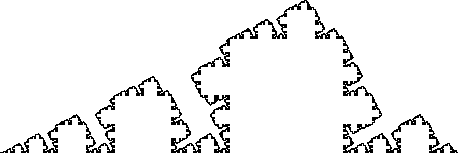
\includegraphics[width=0.75\textwidth]{fractal}
    \end{center}
    \item Repeat parts (c) and (d) for the \emph{area} under the curve at each step. Prove that the area between the fractal curve and the $x$-axis is $\frac 18$.
	\end{enumerate}
\end{enumerate}
%\graphicspath{{notes/7relations/}}

\section{Relations and Partitions}\label{chap:relations}

\iffalse

The mathematics of sets is rather basic, at least until one has a notion of how to relate elements of sets to each other. We are already familiar with examples of this:
\begin{enumerate}
  \item The usual \emph{order} of numbers (e.g. $3<7$) is a way of relating/comparing two elements of $\R$.% Recall that, as sets, order doesn't matter: $\{3,7\}=\{7,3\}$. As \emph{ordered pairs} however, $(3,7)\neq(7,3)$.
  \item A \emph{function} $f:A\to B$ relates elements in a set $A$ with those in $B$.
\end{enumerate}
It turns out that the concept of ordered pair (Cartesian product) is essential to relating elements.

\subsection{Relations}

\begin{defn}
Let $A$ and $B$ be sets. A \emph{(binary) relation} $\cR$ from $A$ to $B$ is a set of ordered pairs
\[\cR\subseteq A\times B.\]
A \emph{relation on} $A$ is a relation from $A$ to itself.\\
If $(x,y)\in\cR$ we can also write $x\,\cR\,y$, and say `$x$ is related to $y$.' Similarly $x\not\!\!\cR\,y$ means $(x,y)\not\in\cR$.
\end{defn}

\begin{examples}
\item $\cR=\{(1,3),(2,2),(2,3),(3,2),(4,1),(5,2)\}$ is a relation from $\N$ to $\N$. It is also a relation from $\{1,2,3,4,5\}$ to $\{1,2,3\}$. Various true statements about this relation include
\[(2,2)\in\cR,\qquad (4,2)\not\in\cR,\qquad 2\not\!\!\cR\,5,\qquad 3\,\cR\,2\]
\item $\cR=\Bigl([1,3)\times (3,4]\Bigr)\cup\big\{(2t+1,t^2):t\in [\frac 12,2]\big\}$ is a relation from $\R$ to $\R$. Be careful: it is easy to confuse interval notation with the notation for ordered pair!
\item The set $\cR=\{(a,a):a\in A\}$ is a relation on $A$, indeed
\[(x,y)\in \cR\iff x=y\]
defines a relation on \emph{any} set $A$. This example is where the term \emph{equivalence relation} (Section \ref{sec:equiv}) comes from. $x\,\cR\,y\iff x=y$ simply says that $\cR$ is `equals.'
\item If $A=\{\text{all humans}\}$, we may define $\cR\subseteq A\times A$ by
\[(a_1,a_2)\in \cR\iff a_1,a_2\text{ have a parent-child, or a sibling relationship.}\]
In this example, the mathematical use of the word relation is identical to that in English. For example, I am related to my sister, and my mother is related to me.
\item If $A$ is a set, then $\subseteq$ is a relation on the power set $\cP(A)$.\\
For example, if $A=\{1,2,3\}$ then $\{1\}\in\cP(A)$ and $\{1,3\}\in\cP(A)$. We'd say that $\{1\}$ is related to $\{1,3\}$ since $\{1\}\subseteq\{1,3\}$.\\
It should be clear that, under the relation $\subseteq$, that $\{1,3\}$ is not related to $\{1\}$.
\end{examples}

When $\cR$ is a relation between sets of numbers, we can often \emph{graph} the relation. Examples 1 and 2 above would be graphed as follows:
\begin{center}
\begin{minipage}{0.3\textwidth}\centering
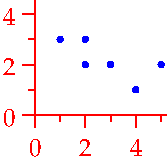
\includegraphics[width=\textwidth]{relations-01-reln1}\\
Example 1.
\end{minipage}\qquad\qquad\qquad
\begin{minipage}{0.3\textwidth}\centering
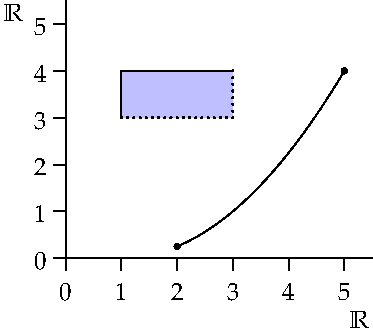
\includegraphics[width=\textwidth]{relations-02-reln2}\\
Example 2.
\end{minipage}
\end{center}
Not all relations between sets of numbers can be graphed: for example, graphing the relation $\cR=\Q\times\Q$ is impossible!\\


\noindent\begin{minipage}{0.6\textwidth}
To refer to the introduction, the standard ordering $<$ on $\N$ is a relation, and we can graph it: for all $x,y\in\N$, we define
\[x\,\cR\,y\iff x<y\]
or equivalently,
\[\cR=\{(x,y)\in\N\times\N:x<y\}\]
\vspace*{10pt}
\end{minipage}\hfill\begin{minipage}{0.3\textwidth}
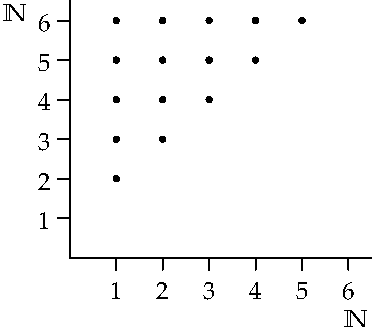
\includegraphics[width=\textwidth]{relations-25-less}
\end{minipage}\\
We can also think about functions in this language: if $f:\R\to\R$ is a function, then we could define
\[x\,\cR\,y\iff y=f(x)\]
or equivalently
\[\cR=\{(x,y)\in\R^2:y=f(x)\}\]
We will return to this viewpoint on function in the Section \ref{sec:func2}.

\subsubsection*{Basic results regarding relations}

With abstract relations, there are only a small number of things we can do.

\begin{defn}\label{defn:relnsym}
If $\cR\subseteq A\times B$ is a relation, then its \emph{inverse} $\cR^{-1}\subseteq B\times A$ is the set
\[\cR^{-1}=\{(y,x)\in B\times A:(x,y)\in\cR\}.\]
To find the elements of $\cR^{-1}$, you simply switch the components of each ordered pair in $\cR$.\\
Suppose $A=B$. We say that $\cR$ is \emph{symmetric} if $\cR=\cR^{-1}$.
\end{defn}\pagebreak[1]

\noindent The following results should seem natural, even if some of the proofs may not be obvious.

\begin{thm}\label{thm:relbasic}
Given any relations $\cR,\cS\subseteq A\times B$:
\begin{enumerate}
\item $(\cR^{-1})^{-1}=\cR$
\item $\cR\subseteq \cS\iff \cR^{-1}\subseteq \cS^{-1}$
\item $(\cR\cup \cS)^{-1}=\cR^{-1}\cup \cS^{-1}$
\item $(\cR\cap \cS)^{-1}=\cR^{-1}\cap \cS^{-1}$
\item If $A=B$, then $\cR\cup \cR^{-1}$ is symmetric
\item If $A=B$, then $\cR\cap \cR^{-1}$ is symmetric
\end{enumerate}
\end{thm}

\begin{proof}
Here are two of the arguments. Try the others yourself.
\begin{enumerate}
\item[2.] Assume that $\cR\subseteq\cS$, and suppose that $(x,y)\in\cR^{-1}$. We must prove that $(x,y)\in\cS^{-1}$. By the definition of inverse,
\begin{align*}
(x,y)\in\cR^{-1}&\implies (y,x)\in\cR\implies (y,x)\in\cS\\
&\implies (x,y)\in\cS^{-1}.
\end{align*}
Therefore $\cR^{-1}\subseteq\cS^{-1}$. For the converse, suppose that $\cR^{-1}\subseteq\cS^{-1}$. Then, by an argument similar to the above, we see that $(\cR^{-1})^{-1}\subseteq (\cS^{-1})^{-1}$. Now use 1.\ to see that
\[\cR^{-1}\subseteq\cS^{-1}\implies\cR\subseteq \cS.\]
\item[5.] By 3,
\[(\cR\cup \cR^{-1})^{-1}=\cR^{-1}\cup (\cR^{-1})^{-1}=\cR^{-1}\cup \cR=\cR\cup \cR^{-1},\]
and so $\cR\cup \cR^{-1}$ is symmetric.\qedhere
\end{enumerate}
\end{proof}

\noindent{\bf Keep your proof skills sharp!}\quad Several parts of Theorem \ref{thm:relbasic} look suspiciously similar to earlier results and it is easy to get confused. For example, 3 and 4 look almost like De Morgan's laws, except that $\cup$ and $\cap$ do not switch over. This is why it is important to be able to conjure up examples and \emph{prove} such statements. There are many facts in mathematics: trying to memorize everything is too difficult! Instead, you will be forever conjecturing and having to justify your guesses. For example, suppose that you forget results 3 and 4: it seems reasonable to conjecture that
\[(\cR\cup \cS)^{-1}=\begin{cases}
\cR^{-1}\cup \cS^{-1}\\
\qquad\text{or}\\
\cR^{-1}\cap \cS^{-1}
\end{cases}\]
Now that you have two sensible guesses, you should be able to decide the correct one by thinking about examples and, if necessary, proving your assertion!

\begin{example}
Consider Example 1 from before: $\cR=\{(1,3),(2,2),(2,3),(3,2),(4,1),(5,2)\}\subseteq\N\times\N$. This is not symmetric since, for example, $1\,\cR\,3$ but $3\not\!\!\cR\,1$. We compute
\[\cR^{-1}=\{(3,1),(2,2),(3,2),(2,3),(1,4),(2,5)\},\]
and observe that
\begin{gather*}
\cR\cap \cR^{-1}=\{(2,2), (2,3), (3,2)\}\quad\text{and}\quad \\
\cR\cup \cR^{-1}=\{(1,3),(3,1),(2,2),(2,3),(3,2),(4,1),(1,4),(5,2),(2,5)\}
\end{gather*}
are both symmetric.
\end{example}

\begin{center}
\begin{minipage}{0.35\textwidth}\centering
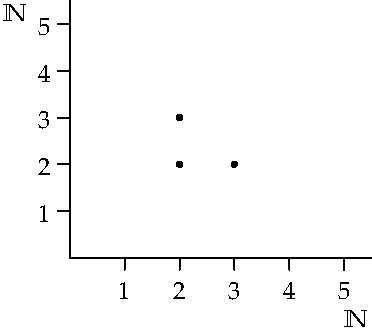
\includegraphics[width=\textwidth]{relations-03-relnint}\\
The relation $\cR\cap \cR^{-1}$
\end{minipage}\qquad\qquad\qquad
\begin{minipage}{0.35\textwidth}\centering
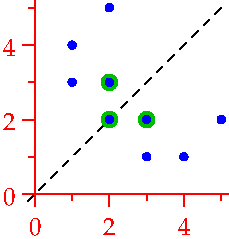
\includegraphics[width=\textwidth]{relations-04-relnun}\\
The relation $\cR\cup \cR^{-1}$
\end{minipage}
\end{center}

\noindent These pictures should confirm something intuitive: if you are able to graph a symmetric relation, then the graph will have symmetry about the line $y=x$. Indeed, $\cR^{-1}$ is obtained by reflecting $\cR$ in the line $y=x$. Recall how to graph an inverse functions from calculus\ldots

\paragraph{Self-test Questions}

	\begin{enumerate}
    \item A \emph{relation} $\cR$ from a set $A$ to a set $B$ is \underline{\phantom{a subset of $A\times B$}\qquad\qquad} 
    \item If $A\subseteq\R$, then the graph of a symmetric relation $\cR\subseteq A\times A$ has what sort of symmetry?
    \item True or false: if $\cR$ is symmetric, then it must contain an even number of elements.
  \end{enumerate}

\subsection*{Exercises}

\begin{enumerate}\renewcommand{\labelenumi}{\thesubsection.\theenumi}
  \item Let $\cR$ be the relation on $\{0,1,2\}$ defined by
  \[0\,\cR\,0\qquad 0\,\cR\,1\qquad 2\,\cR\,1\]
  \begin{enumerate}
    \item Write $\cR$ as a set of ordered pairs.
    \item What is the inverse of $\cR$?
	\end{enumerate}
	
	\item Let $\cR$ be the relation on $\R$ defined by $x\,\cR\,y\iff\nm{x-y}=1$. Draw $\cR$. Is it symmetric?
  
	\item Draw pictures of the following relations on the set of real numbers $\R$.
		\begin{enumerate}
			\item $\cR=\{(x,y):y\le x\text{ and }y\le 2\text{ and }y\le 2-x\}$.
			\item $\cS=\{(x,y):(x-4)^2+(y-1)^2\le 9\}$.
		\end{enumerate}
	Also draw the inverse of each relation.
	
	\item A relation is defined on $\N$ by $a\,\cR\,b\!\iff\! \frac ab\in\N$. Let $c,d\in\N$. Under what conditions is it permissable to write $c\,\cR^{-1}\,d$?
	
	\item Let $\cR\subseteq\{1,2,3,4\}\times\{1,2,3,4\}$ be the relation
	\[\cR=\{(1,3),(1,4),(2,2),(2,4),(3,1),(3,2),(4,4)\}.\]
	\begin{enumerate}
	  \item Compute $\cR^{-1}$.
	  \item Compute the relations $\cR\cup \cR^{-1}$ and $\cR\cap \cR^{-1}$, and check that they are symmetric.
	\end{enumerate}
  
  \item For the relation $\cR=\{(x,y):x\le y\}$ defined on $\N$, what is $\cR^{-1}$, and what is the intersection $\cR\cap\cR^{-1}$?

  \item Let $A$ be a set with $\nm A=4$. What is the maximum number of elements that a relation $\cR$ on $A$ can contain such that $\cR\cap \cR^{-1}=\emptyset$?
  
  \item Give formal proofs of the remaining cases (1, 3, 4 \& 6) of Theorem \ref{thm:relbasic}.
  
  \item Let $\cR$ be a relation on a set $A$ and define $\cS=\cR\cup\cR^{-1}$. We know that $\cS$ is symmetric. Prove that $\cS$ is the intersection of all \emph{symmetric} relations on $A$ which contain $\cR$. Otherwise said: if
  \[\mathrm T=\Bigl\{\mathcal T\subseteq A\times A:\mathcal T\text{ symmetric and }\cR\subseteq\mathcal T\bigr\}\]
  then
  \[\cS=\bigcap\limits_{\mathcal T\in \mathrm T} \mathcal T\]
  \emph{$\cS$ is known as the \emph{symmetric closure} of $\cR$.}
\end{enumerate}
\newpage


\subsection{Functions revisited}\label{sec:func2}

Now that we have the language of relations, we can properly define functions. Recall that a function $f:A\to B$ is a rule that assigns one, and only one, element of $B$ to each element of $A$. We may therefore view $f$ as a collection of ordered pairs in $A\times B$:
\[\big\{(a,f(a)):a\in A\big\}.\]
This set is nothing more than the \emph{graph} of the function, and, being a set of ordered pairs, it is a relation.

\begin{defn}\label{defn:func}
Let $\cR\subseteq A\times B$ be a relation from $A$ to $B$. The \emph{domain} and \emph{range} of $\cR$ are the sets
\begin{gather*}
\dom(\cR)=\{a\in A:(a,b)\in \cR\text{ for some }b\in B\},\\
\range(\cR)=\{b\in B:(a,b)\in \cR\text{ for some }a\in A\}.
\end{gather*}
A \emph{function} from $A$ to $B$ is a relation $f\subseteq A\times B$ satisfying the following conditions:
\begin{enumerate}
  \item $\dom(f)=A$,
  \item $(a,b_1),(a,b_2)\in f\implies b_1=b_2$.
\end{enumerate}
\end{defn}

\noindent The two conditions can be thought of as saying:
\begin{enumerate}
  \item Every element of $A$ is related to \emph{at least one} element of $B$.
  \item Every element of $A$ is related to \emph{at most one} element of $B$.
\end{enumerate}
Putting these together, we see that a relation $f\subseteq A\times B$ is a function if \emph{every} $a\in A$ is the first entry of one (and only one) ordered pair $(a,b)\in f$. The second condition is the vertical line test, familiar from calculus.

\begin{center}
\begin{minipage}{0.32\textwidth}\centering
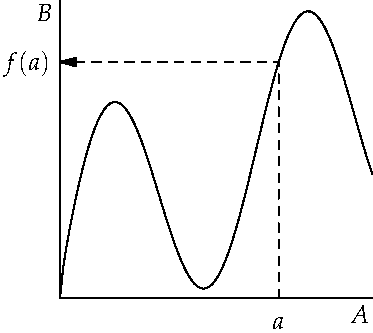
\includegraphics[width=\textwidth]{relations-05-funcvert}\\
$b_1=b_2=f(a)$: a function
\end{minipage}\qquad\qquad\qquad\qquad
\begin{minipage}{0.32\textwidth}\centering
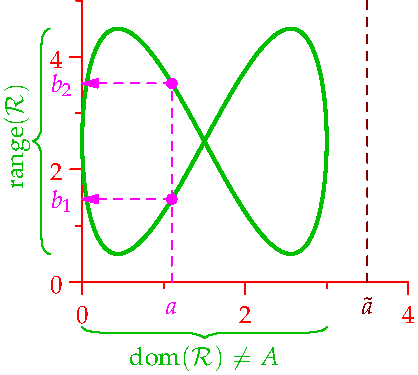
\includegraphics[width=\textwidth]{relations-06-funcvert}\\
$b_1\neq b_2$: not a function
\end{minipage}
\end{center}

\noindent We can also think about injectivity and surjectivity (recall Definition \ref{defn:11}) in this context. A function $f\subseteq A\times B$ is:
\begin{itemize}
  \item \emph{Injective} if no two pairs in $f$ share the same second entry.
  \item \emph{Surjective} if every $b\in B$ appears as the second entry of at least one pair in $f$.
  \item \emph{Bijective} if every $b\in B$ appears as the second entry of one (and only one) ordered pair $(a,b)\in f$.
\end{itemize}


\begin{example}
Let $A=B=\{1,2,3\}$ and consider the relation\\
\noindent\begin{minipage}{0.62\textwidth}
\[f=\{(1,3),(2,1),(3,3)\}.\]
Observe that $\dom(f)=\{1,2,3\}=A$, and that each element of $A$ appears exactly once as the first element in a pair $(a,b)\in f$. The relation therefore satisfies both conditions necessary to be a function. In more elementary language we would write $f(1)=3$, \ $f(2)=1$ and $f(3)=3$.\\[5pt]
Since 3 appears twice as a second entry of an ordered pair in $f$ we see that $f$ is \emph{not injective.}\\[5pt]
Since 2 never appears as the second entry of an ordered pair in $f$ we see that $f$ is \emph{not surjective.}
\end{minipage}\hfill\begin{minipage}{0.33\textwidth}
\centering
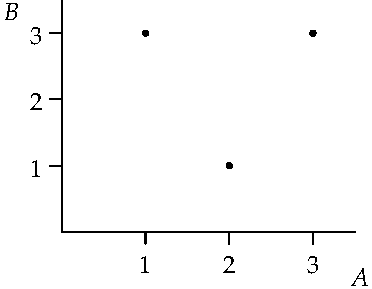
\includegraphics[width=\textwidth]{relations-18-reln1}\\
A function $f:A\to B$
\end{minipage}
\end{example}

\subsubsection*{The Inverse of a Function}

Since every function is a relation, it is a straightforward business to define the inverse of a function.

\begin{defn}
The \emph{inverse} of a function $f\subseteq A\times B$ is the inverse relation $f^{-1}\subseteq B\times A$.
\end{defn}

\noindent To compute an inverse relation we simply reverse the components of each ordered pair: the following should therefore be clear.

\begin{thm}\label{thm:inversedomrange}
$\dom(f^{-1})=\range(f)$ \ and \ $\range(f^{-1})=\dom(f)$.
\end{thm}

\noindent In general, you should expect the inverse of a function to be merely a relation and not a function in its own right. We shall shortly (Theorem \ref{thm:finverse}) discuss when the inverse relation is a function.

\begin{example}[cont.]
Consider the above example.\\[5pt]
\noindent\begin{minipage}{0.62\textwidth}
The inverse relation
\[f^{-1}=\{(3,1),(1,2),(3,3)\}\subseteq B\times A\]
is \emph{not} a function due to failing \emph{both} conditions of Definition \ref{defn:func}.
\begin{itemize}
  \item $\dom(f^{-1})=\{1,3\}$ is not the whole of $B$.
  \item $(3,1)\in f^{-1}$ and $(3,3)\in f^{-1}$, but $1\neq 3$.
\end{itemize}
Both failures are clearly visible in the picture.
\end{minipage}\hfill\begin{minipage}{0.33\textwidth}
\centering
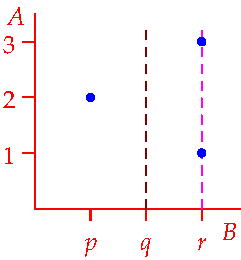
\includegraphics[width=\textwidth]{relations-19-reln1}\\
$f^{-1}\subseteq B\times A$: not a function
\end{minipage}
\end{example}

\noindent Before we consider exactly when the inverse of a function is a function in its own right, we consider a few more examples.


\begin{examples}
\item\label{ex:reln1} Let $A=B=\R$ and $f=\{(x,x^2):x\in\R\}$. This is simply the function with formula $f(x)=x^2$. The inverse relation $f^{-1}\subseteq\R\times\R$ is then
\[f^{-1}=\bigl\{(x^2,x):x\in\R\bigr\}=\bigl\{(y,\pm\sqrt y):y\ge 0\bigr\}.\]
In this case, $f^{-1}$ is \emph{not a function.} In the language of Definition \ref{defn:func}:
\begin{itemize}
  \item $\dom(f^{-1})=\R^+_0\neq B$. E.g., $-1\in B$ but $-1\not\in\dom(f^{-1})$.
  \item $(4,2)$ and $(4,-2)$ are distinct elements of $f^{-1}$ with the same first entry.
\end{itemize}
\begin{center}
\begin{minipage}{0.35\textwidth}\centering
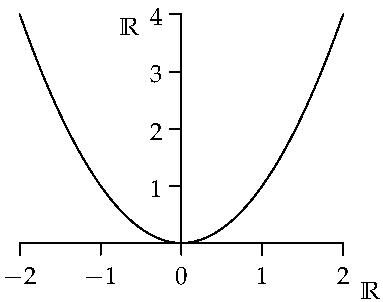
\includegraphics[width=\textwidth]{relations-20-reln2}\\
$f:A\to B$
\end{minipage}\qquad\qquad\qquad
\begin{minipage}{0.35\textwidth}\centering
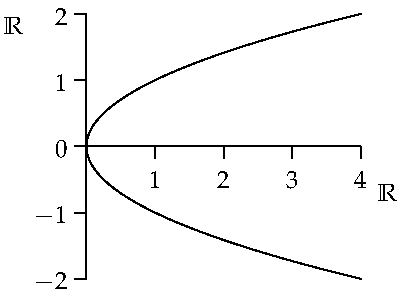
\includegraphics[width=\textwidth]{relations-21-reln2}\\
$f^{-1}\subseteq B\times A$: not a function
\end{minipage}
\end{center}
It should be obvious that $f$ is neither injective nor surjective: in the language of relations,
\begin{description}
	\item[Not injective]\quad $(2,4)$ and $(-2,4)$ are distinct elements of $f$ with the same second entry.
	\item[Not surjective]\quad For instance, $-1$ never appears as the second entry of any pair in $f$.
\end{description}
Observe how these are merely a rewriting of what it means for $f^{-1}$ to fail to be a function.

\item\label{ex:reln2} Let $A=B=\R$ and $f=\{(x,x^3):x\in\R\}$, so that $f$ has formula $f(x)=x^3$. This time, the inverse is also a function and we could write $f^{-1}(y)=\sqrt[3]{y}$:
\[f^{-1}=\bigl\{(x^3,x):x\in\R\bigr\}=\bigl\{(y,\sqrt[3]{y}):y\in\R\bigr\}.\]
\begin{center}
\begin{minipage}{0.35\textwidth}\centering
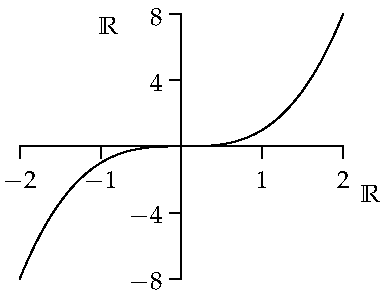
\includegraphics[width=\textwidth]{relations-22-reln3}\\
$f:A\to B$
\end{minipage}\qquad\qquad\qquad
\begin{minipage}{0.35\textwidth}\centering
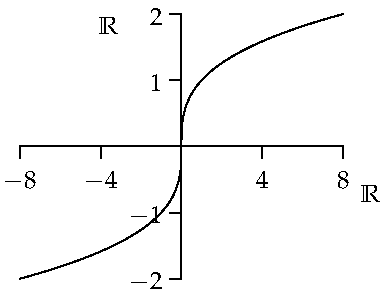
\includegraphics[width=\textwidth]{relations-23-reln3}\\
$f^{-1}:B\to A$ is a function
\end{minipage}
\end{center}
\end{examples}\pagebreak[2]

\noindent All three of our examples help to illustrate the following important result.

\begin{thm}\label{thm:finverse}
A relation $f^{-1}\subseteq B\times A$ is a function $\iff f$ is bijective (both injective and surjective).
\end{thm}

\begin{proof}
Recalling Definition \ref{defn:func}, we see that
\[f^{-1}\text{ is a function }\iff\begin{cases}
\dom(f^{-1})=B,\\
\qquad\text{\emph{and}}\\
(b,a_1),(b,a_2)\in f^{-1}\implies a_1=a_2.
\end{cases}\]
The first of these is equivalent to $\range(f)=B$, which says that $f$ is surjective.\\
The second is equivalent to $(a_1,b),(a_2,b)\in f\implies a_1=a_2$, which says that $f$ is injective.
\end{proof}

\noindent Here is a final example, where the function $f$ is harder to visualize.

\begin{example}
Let $A=\R$, $B=\Q$ and define $f$ using the formula 
\[f(x)=\begin{cases}
x&\text{if }x\in\Q,\\
0&\text{if }x\not\in\Q.
\end{cases}\]
In the language of relations, this is $f=\bigl\{(x,x):x\in\Q\bigr\}\cup\bigl\{(x,0):x\not\in\Q\bigr\}$.\\[2pt]
This is a surjective function since every element of $B=\Q$ appears as the second entry in an ordered pair $(a,b)\in f$. It is not injective since zero appears more than once in the second entry. For example,
\[(\sqrt 2,0),\ (\sqrt 3,0)\in f.\]
Written in the more common manner, we are observing that $f(\sqrt 3)=f(\sqrt 2)$.\\[2pt]
The inverse $f^{-1}$ is not a function, and it fails to be so precisely because $f$ is non-injective. For example
\[(0,\sqrt 2)\text{ and } (0,\sqrt 3)\text{ are distinct elements of $f^{-1}$ with the same  first component.}\]
\end{example}

\paragraph{Inverse Images}

Analogously to the concept of images of sets (Section \ref{sec:func1}), we can define the \emph{inverse image} of a subset $V\subseteq B$ under a function $f:A\to B$ by
\[f^{-1}(V)=\{a\in A:f(a)\in V\}.\]
In particular, if $\{b\}\subseteq B$ has only one element, then its inverse image is
\[f^{-1}(\{b\})=\{a\in A:f(a)=b\}.\]
Both are \emph{subsets} of $A$. For instance, in the last example the inverse image of $\{0\}$ consists of zero and all irrational numbers!
\[f^{-1}(\{0\})=\{0\}\cup(\R\setminus\Q)\]
When $f^{-1}\subseteq B\times A$ is a function, each inverse image of a singleton consists of one point of $A$: thus $f^{-1}(\{b\})=\{a\}$. \emph{Only} in such a case are we entitled to write $f^{-1}(b)=a$.\pagebreak[2]




\begin{aside}
\noindent{\bf Equality of functions}

There are two competing notions of what it means for two functions to be \emph{equal.}

\begin{description}
\item[Same domain, same graph, same codomain]\quad $f=g$ means that $f$ and $g$ are the same subset of the \emph{same} $A\times B$. This notion is preferred by set theorists because it sticks rigidly to the idea that a function is a \emph{relation,} and it requires both the domain $A$ and codomain $B$ to be explicit.
\item[Same domain, same graph]\quad $f=g$ means that $f\subseteq A\times B$, \ $g\subseteq A\times C$, and
\[(a,b)\in f\iff (a,b)\in g.\]
This notion considers what a function \emph{does} to be fundamental; if two functions do the same thing to elements of the same domain then they are the same. This looser notion of equality is used more often, especially in elementary calculus.
\end{description}

\noindent The second conception of equality, while intuitive, has a problem. For example, let
\[f:\R\to\R,\quad\text{and}\quad g:\R\to[-1,1]\quad\text{satisfy}\quad f(x)=g(x)=\sin x.\]
Although $f$ and $g$ have the same graph, the different codomains of $f$ and $g$ mean that these are \emph{different functions} with respect to the first notion. Under the second notion, they are the \emph{same function.} However, $g$ is surjective while $f$ is not, so wouldn't we prefer $f$ and $g$ to be non-equal?\footnote{In elementary calculus, we usually say that a function is invertible if it is 1--1. In order for this to make sense, we have to ignore surjectivity and use the second notion of functional equality.}\\


\noindent The same problem does not arise when considering domains. For example, in calculus you might have compared functions such as
\[f(x)=x^2+2,\quad\text{and}\quad g(x)=\frac{(x^2+2)(x-1)}{x-1}.\]
The implied domains of these functions are $\dom(f)=\R$ and $\dom(g)=\R\setminus\{1\}$. Even though these have the same graph whenever \emph{both} are defined, regardless of which notion you choose we have $f\neq g$, since the functions have \emph{different domains.}
\end{aside}

\paragraph{Self-test Questions}

	\begin{enumerate}
    \item What does it mean for a \emph{relation} $\cR\subseteq A\times B$ to be a \emph{function}?
    \item If $f\subseteq A\times B$ is a function, what does it mean, in the language of relations, for $f$ to be \emph{injective}? \emph{Surjective}?
    \item True or false: a relation $\cR$ has a domain and range if and only if it is a function.
  \end{enumerate}


\subsection*{Exercises}

\begin{enumerate}\renewcommand{\labelenumi}{\thesubsection.\theenumi}
  \item Suppose that $f\subseteq\{1,2,3,4\}\times\{1,2,3,4,5,6,7\}$ is the relation
  \[f=\{(1,1),(2,3),(3,5),(4,7)\}.\]
  \begin{enumerate}
    \item Show that $f$ is a function $f:\{1,2,3,4\}\to\{1,2,3,4,5,6,7\}$. Can you find a concise formula $f(x)$ to describe $f$?
    \item Is $f$ injective? Justify your answer.
    \item Suppose that $g\subseteq\{1,2,3,4\}\times B$ is another relation so that the \emph{graphs} of $f$ and $g$ are identical: i.e.
    \[\bigl\{(a,f(a)):a\in\{1,2,3,4\}\bigr\}=\bigl\{(a,g(a)):a\in\{1,2,3,4\}\bigr\}.\] \emph{as sets.} If $g$ is a bijective function, what is $B$?
  \end{enumerate}
  
  \item Decide whether each of the following relations are functions. For those which are, decide whether the function is injective and/or surjective.
  \begin{enumerate}
    \item $\cR=\{(x,y)\in[-1,1]\times[-1,1]:x^2+y^2=1\}$
    \item $\cS=\{(x,y)\in[-1,1]\times[0,1]:x^2+y^2=1\}$
    \item $\mathcal T=\{(x,y)\in[0,1]\times[-1,1]:x^2+y^2=1\}$
    \item $\mathcal U=\{(x,y)\in[0,1]\times[0,1]:x^2+y^2=1\}$
  \end{enumerate}
  
  \item In Example \ref{ex:reln2} on page \pageref{ex:reln2}, explain why the function $f$ is both injective and surjective using the language of relations: i.e., in the same manner as we analyzed Example \ref{ex:reln1}.
  
  \item For each of the examples on page \pageref{ex:reln2}, compute the following inverse images:
  \begin{enumerate}
    \item $f^{-1}(\{0,1\})$
    \item $f^{-1}\Big([0,1)\Big)$
    \item $f^{-1}\Big((-\infty,0]\Big)$
    \item $f^{-1}\Big(\{-8\}\cup[-7,2]\cup (3,9)\Big)$
  \end{enumerate}
  
  \item\begin{enumerate}
    \item Express the function $f:\R\to\R:x\mapsto x^4+3$ as a relation.
    \item What is the inverse relation $f^{-1}$?
    \item Use Definition \ref{defn:func} to prove that the relation $f^{-1}$ is \emph{not} a function.
    \item Prove directly from Definition \ref{defn:11} that $f$ is not injective and not surjective. Compare your arguments with your answer to part (c).
  \end{enumerate}
  
  \item Repeat the previous question for $f:\R\to\R:x\mapsto \sqrt{x^2-4x+5}$.
  
  \item Give a formal proof of Theorem \ref{thm:inversedomrange}.
  
  \item Prove or disprove the following: if $f:A\to B$ is a function, and $U,V\subseteq B$, then
  \[f^{-1}(U\cap V)=f^{-1}(U)\cap f^{-1}(V)\]
\end{enumerate}
\newpage

\subsection{Equivalence Relations}\label{sec:equiv}

In mathematics, the notion of \emph{equality} is not as simple as one might think. The idea of two numbers being equal is straightforward, but suppose we want to consider two paths between given points as `equal' if and only if they have the same length? Since two `equal' paths might look very different, is this a good notion of equality? Mathematicians often want to gather together objects that have a common property and then treat them as if they were a single object. This is done using equivalence relations and equivalence classes.\\

\noindent First recall the alternative notation for a relation on a set $A$: if $\cR\subseteq A\times A$ is a relation on $A$, then $x\,\cR\,y$ has the same meaning as $(x,y)\in\cR$. We might read $x\,\cR\,y$ as `$x$ is $\cR$-related to $y$.'

\newsavebox\mybox
\sbox{\mybox}{\emph{Transitivity}}
\def\refl{\makebox[\wd\mybox][l]{\emph{Reflexivity}}}
\def\symm{\makebox[\wd\mybox][l]{\emph{Symmetry}}}
\def\trans{\makebox[\wd\mybox][l]{\emph{Transitivity}}}

\begin{defn}
A relation $\cR$ on a set $A$ may be described as \emph{reflexive, symmetric} or \emph{transitive} if it satisfies the following properties:
	\begin{ptabular}{\trans}
		\refl&$\forall x\in A$, \ $x\,\cR\,x$\hfill(every element of $A$ is related to itself)\\
		\symm&$\forall x,y\in A,\ x\,\cR\,y\implies y\,R\,x$\hfill(if $x$ is related to $y$, then $y$ is related to $x$)\\
		\trans&$\forall x,y,z\in A,\ x\,\cR\,y$ \ and \ $y\,\cR\,z\implies x\,\cR\,z$\hfill(if $x$ is related to $y$, and $y$ is related to $z$,\newline
		\phantom{bob}\hfill then $x$ is related to $z$)
	\end{ptabular}
\end{defn}

Symmetry is exactly the same notion as in Definition \ref{defn:relnsym}.

\begin{examples}
\item Let $A=\R$ and let $\cR$ be $\le$. Thus $2\le 3$, but $7\nleq 4$. We check whether $\cR$ satisfies the above properties.
	\begin{eptabular}{\trans}
		\refl&True. $\forall x\in\R$, \ $x\le x$.\\
		\symm&False. For example, $2\le 3$ but $3\nleq 2$.\\
		\trans&True. $\forall x,y,z\in\R$, if $x\le y$ and $y\le z$, then $x\le z$.
	\end{eptabular}
\item Let $A$ be the set of lines in the plane and define $\ell_1\,R\,\ell_2\iff \ell_1$ and $\ell_2$ intersect.\\
\noindent\begin{minipage}{0.65\textwidth}
	\noindent\begin{eptabular}{\trans}
		\refl&True. Every line intersects itself, so $\ell\,\cR\,\ell$ for all $\ell\in A$.\\
		\symm&True. For all lines $\ell_1,\ell_2\in A$, if $\ell_1$ intersects $\ell_2$, then $\ell_2$ intersects $\ell_1$..\\
		\trans&False. As the picture illustrates, we may let $\ell_1$ and $\ell_3$ be parallel lines, and $\ell_2$ cross both of these. Then $\ell_1\,\cR\,\ell_2$ and $\ell_2\,\cR\,\ell_3$, but $\ell_1\not\!\!\cR\,\ell_3$.
	\end{eptabular}
\end{minipage}\hfill
		\begin{minipage}{0.3\textwidth}
	\includegraphics[width=\textwidth]{relations-07-parallel}
		\end{minipage}
\end{examples}

\begin{defn}
An \emph{equivalence relation} is a relation $\sim$ which is reflexive, symmetric and transitive.
\end{defn}

\noindent The symbol $\sim$ is almost universally used for an abstract equivalence relation. It can be read as `related to,' `tilde,' or `twiddles.' The two examples above are \emph{not} equivalence relations because they fail one of the three conditions. We now exhibit the simplest equivalence relation.

\begin{example}
Equals `=' is an equivalence relation on any set, hence the name!
\end{example}

\noindent Read the definitions of reflexive, symmetric and transitive until you are certain of this fact. There are countless other equivalence relations: here are a few.

\begin{examples}
	\item For all $x,y\in\Z$, we define the relation $\sim$ by
	\[x\sim y\iff x-y\ \text{ is even.}\]
	We claim that $\sim$ is an equivalence relation on $\Z$.
	\begin{eptabular}{\trans}
		\refl&$\forall x\in\Z,\ x-x=0$ is even, hence $x\sim x$.\\
		\symm&$\forall x,y\in\Z,\ x\sim y\implies x-y$ is even $\implies y-x$ is even $\implies y\sim x$.\\
		\trans&$\forall x,y,z\in\Z$, if $x\sim y$ and $y\sim z$, then $x-y$ and $y-z$ are even. But the sum of two even numbers is even, hence $x-z=(x-y)+(y-z)$ is even, and so $x\sim z$.
	\end{eptabular}
	
	\item Let $A=\{$all students taking this course$\}$. For all $x,y\in A$, let
	\[x\sim y\iff x\ \text{ achieves the same letter-grade as $y$.}\]
	Then $\sim$ is an equivalence relation on $A$; here is the proof.
	\begin{eptabular}{\trans}
		\refl&$\forall x\in A,\ x\sim x$ since everyone scores the same as themself!\\
		\symm&$\begin{array}[t]{@{}rl}
		\forall x,y\in A,\ x\sim y&\implies x\ \text{achieves the same letter-grade as $y$}\\
		&\implies y\ \text{achieves the same letter-grade as $x$}\\
		&\implies y\sim x
		\end{array}$\\
		\trans&$\forall x,y,z\in A$, if $x\sim y$ and $y\sim z$, then $x$ achieves the same as $y$ who achieves the same as $z$, whence $x$ achieves the same as $z$. Thus $x\sim z$.
	\end{eptabular}

	\item We define an equivalence relation on $\Z$ by
	\[\forall x,y\in\Z,\ \ x\sim y\iff x^2\equiv y^2\pmod 5.\]
		\begin{eptabular}{\trans}
		\refl&$\forall x\in\Z,\ x\sim x$ since $x^2$ is always congruent to itself!\\
		\symm&$\begin{array}[t]{@{}rl}
		\forall x,y\in\Z,\ x\sim y&\implies x^2\equiv y^2\pmod 5\\
		&\implies y^2\equiv x^2\pmod 5\\
		&\implies y\sim x
		\end{array}$\\
		\trans&$\forall x,y,z\in\Z$, if $x\sim y$ and $y\sim z$, then $x^2\equiv y^2$ and $y^2\equiv z^2\pmod 5$. But then $x^2\equiv z^2\pmod 5$ and so $x\sim z$.
	\end{eptabular}
\end{examples}

\noindent The most important thing to observe in each of these examples is that {\bf an equivalence relation separates elements of a set into subsets where elements share a common property} (even/oddness, letter-grade, etc.). The next definition formalizes this idea.

\begin{defn}\label{defn:equivrel}
Let $\sim$ be an equivalence relation on a set $X$. The \emph{equivalence class} of an element $x\in X$ is the set
\[[x]=\{y\in X:y\sim x\}.\]
Otherwise said, $y\sim x\iff y\in[x]$. The set of all equivalence classes is known as the \emph{quotient} of $X$ by $\sim$ or simply `$X$ mod $\sim$,' and is denoted
\[\quotient X\sim=\Big\{[x]:x\in X\Big\}\]
\end{defn}

\noindent Let us think about the definition of equivalence class in the context of our previous examples.

\begin{examples}
	\item $[0]=\{y\in\Z:y\sim 0\}=\{y\in\Z:y\text{ is even}\}$ is the set of even numbers. Note that $[0]=[2]=[4]=[6]$, etc. The other equivalence class is $[1]=\{y\in\Z:y-1\text{ is even}\}$, which is the set of odd numbers. The quotient set is
	\[\smash{\quotient \Z\sim}=\bigl\{[0],[1]\bigr\}=\bigl\{\{\text{even numbers}\},\{\text{odd numbers}\}\bigr\}.\]

	\item There is one equivalence class for each letter grade awarded. Each equivalence class contains all the students who obtain a particular letter-grade. If we call the equivalence classes $\mathrm{A^+,A,A^-,B^+,\ldots,F}$, where, say, $\mathrm B=\{$students obtaining a B-grade$\}$, then
	\[\smash{\quotient{\{\text{Students}\}}{\sim}}=\{\mathrm{A^+,A,A^-,B^+,\ldots,F}\}.\]

	\item The equivalence classes for this example are a little tricky. First observe that
	\[x\equiv y\tpmod 5\implies x^2\equiv y^2\tpmod 5,\]
	so that there are at most five equivalence classes; those of 0, 1, 2, 3 and 4. Are they distinct?	If we square each of these and consider the remainder modulo 5, we obtain
	\[\begin{array}{l@{}r|c|c|c|c|c}
	x&\tpmod 5&0&1&2&3&4\\\hline
	x^2&\tpmod 5&0&1&4&4&1
	\end{array}\]
	Notice that $1\sim 4$, so they share an equivalence class. Similarly $2\sim 3$. Indeed the distinct equivalence classes are
	\begin{gather*}
	[0]=\{x\in\Z:x\equiv 0\tpmod 5\}\\
	[1]=\{x\in\Z:x\equiv 1,4\tpmod 5\}\\
	[2]=\{x\in\Z:x\equiv 2,3\tpmod 5\}
	\end{gather*}
	In this case the quotient is the set
	\[\smash{\quotient{\Z}{\sim}}=\Bigl\{[0],[1],[2]\Bigr\}.\]
\end{examples}%\pagebreak[2]

\noindent Here is one further example of an equivalence relation, this time on $\R^2$. Be careful with the notation: $\R^2=\R\times\R$ is already a Cartesian product, so a relation on $\R^2$ is a subset of $\R^2\times\R^2$!


\begin{example}\label{ex:equivcircle}
Let $\sim$ be the relation on $\R^2$ defined by $(x,y)\sim(v,w)\iff x^2+y^2=v^2+w^2$. We claim that this is an equivalence relation.
	\begin{ptabular}{\trans}
		\refl&$\forall (x,y)\in\R^2,\ x^2+y^2=x^2+y^2$.\\
		\symm&$\begin{array}[t]{@{}rl}
		\forall (x,y),(v,w)\in\R^2,\ (x,y)\sim(v,w)&\implies x^2+y^2=v^2+w^2\\
		&\implies v^2+w^2=x^2+y^2\\
		&\implies (v,w)\sim(x,y)
		\end{array}$\\
		\trans&$\forall (x,y),(v,w),(p,q)\in\R^2$, if $(x,y)\sim (v,w)$ and $(v,w)\sim (p,q)$, then $x^2+y^2=v^2+w^2$ and $v^2+w^2=p^2+q^2$. But then $x^2+y^2=p^2+q^2$ and so $(x,y)\sim (p,q)$.
	\end{ptabular}\\
	
	$\sim$ is therefore an equivalence relation. But what are the equivalence classes? By definition,
\[[(x,y)]=\Bigl\{(v,w)\in\R^2:v^2+w^2=x^2+y^2\Bigr\}.\]
\noindent\begin{minipage}{0.6\textwidth}
This isn't particularly helpful. Indeed it is easier to think of each of these sets as
\[\Bigl\{(v,w)\in\R^2:v^2+w^2\text{ is \emph{constant}}\Bigr\}.\]
Each equivalence class is therefore a \emph{circle} centered at the origin! Some of the equivalence classes are drawn in the picture: the class $[(1,0)]$ is highlighted. Moreover, the quotient set is
\[\quotient{\R^2}{\sim}=\{\text{circles centered at the origin}\}.\]
\end{minipage}\qquad
\begin{minipage}{0.35\textwidth}
\includegraphics[width=\textwidth]{relations-24-circles}
\end{minipage}
\end{example}

\paragraph{Self-test Questions}

	\begin{enumerate}
    \item True or false: a relation $\sim$ on a set $X$ is \emph{reflexive} if $\exists x\in X$ such that $x\sim x$.
   	\item An \emph{equivalence relation} satisfies which three properties? What do they mean?
    \item Suppose that $x,y,z\in X$ and $\sim$ is an equivalence relation on $X$. Express each of the following assertions in terms of the properties satisfied by an equivalence relation.
    \begin{enumerate}
      \item $x\in[y]$ and $y\in[z]\implies x\in[z]$.
      \item $x\in[x]$.
      \item $x\in[y]\iff y\in[x]$.
  	\end{enumerate}
  \end{enumerate}

\subsection*{Exercises}

\begin{enumerate}\renewcommand{\labelenumi}{\thesubsection.\theenumi}
	\item A relation $\cR$ is \emph{antisymmetric} if $((x,y)\in \cR)\wedge((y,x)\in \cR)\implies x=y$. Give examples of relations $\cR$ on $A=\{1,2,3\}$ having the stated property.
	\begin{enumerate}
		\item $\cR$ is both symmetric and antisymmetric.
		\item $\cR$ is neither symmetric nor antisymmetric.
		\item $\cR$ is transitive but $\cR\cup \cR^{-1}$ is not transitive.
	\end{enumerate}
	
	\item Let $\cS=\{(x,y)\in\R^2:\sin^2x+\cos^2y=1\}$.
	\begin{enumerate}
	  \item Give an example of two real numbers $x,y$ such that $x\,\cS\,y$.
	  \item Is $\cS$ reflexive? Symmetric? Transitive? Justify your answers.
	\end{enumerate}

	\item Each of the following relations $\sim$ is an equivalence relation on $\R^2$. Identify the equivalence classes and draw several of them.
	\begin{enumerate}
		\item $(a,b)\sim(c,d)\iff ab=cd$.
	  \item $(v,w)\sim(x,y)\iff v^2w=x^2y$.
	\end{enumerate}
	
  \item\begin{enumerate}
  \item Let $\sim$ be the relation defined on $\Z$ by $a\sim b\iff a+b$ is even. Show that $\sim$ is an equivalence relation and determine the distinct equivalence classes.
  \item Suppose that `even' is replaced by `odd' in part (a). Which of the properties reflexive, symmetric, transitive does $\sim$ possess?
  \end{enumerate}

  \item For each of the following relations $\cR$ on $\Z$, decide whether $\cR$ is reflexive, symmetric, or transitive, and whether $\cR$ is an equivalence relation.
	\begin{enumerate}
		\item $a\,\cR\,b \iff a\equiv b\pmod 3 \textbf{ or } a\equiv b\pmod 4$.
		\item $a\,\cR\,b \iff a\equiv b\pmod 3 \textbf{ and } a\equiv b\pmod 4$.
	\end{enumerate}

	\item For the purposes of this question, we call a real number $x$ \emph{small} if $\nm x\le 1$. Let $\cR$ be the relation on the set of real numbers defined by
	\[x\,\cR\,y \iff x-y \text{ is small}.\]
	\emph{Prove or disprove}: $\cR$ is an equivalence relation on $\R$.

	\item Let $A=\{1,2,3,4,5,6\}$. The distinct equivalence classes resulting from an equivalence relation $\sim$ on $A$ are $\{1,4,5\}$, $\{2,6\}$, and $\{3\}$. What is $\sim$? Give your answer as a subset of $A\times A$.

	\item $\subseteq$ is a relation on any set of sets. Is $\subseteq$ reflexive, symmetric, transitive? Prove your assertions.

	\item Let $S$ be the set of all polynomials of degree at most 3. An element $s\in S$ can then be expressed as
  \[s(x)=ax^3+bx^2+cx+d,\qquad\text{where $a,b,c,d\in\R$.}\]
  A relation $\cR$ on $S$ is defined by
  \[p\,\cR\,q\iff p\text{ and $q$ have a common root.}\]
  For example $p(x)=(x-1)^2$ and $q(x)=x^2-1$ have the root 1 in common so that $p\,\cR\,q$. Determine which of the properties reflexive, symmetric and transitive are possessed by $\cR$.

  \item Let $A=\{2^m:m\in\Z\}$. A relation $\sim$ is defined on the set $\Q^+$ of positive rational numbers by
  \[a\sim b\iff \frac ab\in A\]
  \begin{enumerate}
    \item Show that $\sim$ is an equivalence relation.
    \item Describe the elements in the equivalence class $[3]$.
  \end{enumerate}

  \item A relation is defined on the set $A=\{a+b\sqrt 2:a,b\in\Q,\,a+b\sqrt 2\neq 0\}$ by $x\sim y\iff \frac xy\in\Q$. Show that $\sim$ is an equivalence relation and determine the distinct equivalence classes.

	\item The \emph{reflexive, symmetric} and \emph{transitive closures} of a relation $\cR$ are defined respectively as the smallest relations containing $\cR$ which also exhibit the given property. Find each of the three closures of $\cR=\{(1,2),(2,3),(3,3)\}\subseteq\Z\times\Z$.

	\item Recall the description of the real projective line (page \pageref{ex:projline}): if $A_m$ is the line through the origin with gradient $m$, then
	\[\pr(\R^2)=\{A_m:m\in\R\cup\{\infty\}\}.\]
	Define a relation $\sim$ on $\R^2_*=\R^2\setminus\{(0,0)\}$ by $(a,b)\sim(c,d)\iff ad=bc$.
	\begin{enumerate}
	  \item Prove that $\sim$ is an equivalence relation.
	  \item Find the equivalence classes of $\sim$. How do the equivalence classes differ from the lines $A_m$?
	\end{enumerate}
  
	\item Suppose that $\cR,\cS$ are relations on some set $X$. Define the \emph{composition} $\cR\circ \cS$ to be the relation
	\[(a,c)\in \cR\circ \cS\iff \exists b\in X\text{ such that }(a,b)\in \cR\text{ and }(b,c)\in \cS.\]
	\begin{enumerate}
		\item If $\cR=\{(1,1),(1,2),(2,3),(3,1),(3,3)\}$ and $\cS=\{(1,2),(1,3),(2,1),(3,3)\}$, find $\cR\circ \cS$.
		\item Suppose that $\cR$ and $\cS$ are reflexive. Prove that $\cR\circ \cS$ is reflexive.
		\item Suppose that $\cR$ and $\cS$ are symmetric. Prove that $(x,y)\in \cR\circ \cS\iff (y,x)\in \cS\circ \cR$.
		\item Give an example of symmetric relations $\cR,\cS$ such that $\cR\circ \cS$ is \emph{not} symmetric. Conclude that if $\cR,\cS$ are equivalence relations, then $\cR\circ \cS$ need not be an equivalence relation.
	\end{enumerate}

  \item (\emph{Only for those who have studied Linear Algebra}) Let $\sim$ be the relation on the set of $2\times 2$ real matrices given by $A\sim B\iff\exists M$ such that $B=MAM^{-1}$.
  \begin{enumerate}
    \item Prove that $\sim$ is an equivalence relation.
    \item What is the equivalence class of the identity matrix?
    \item Show that $\left(\begin{smallmatrix}
    -11&15\\-5&9
    \end{smallmatrix}\right)\sim \left(\begin{smallmatrix}
    4&10\\0&-6
    \end{smallmatrix}\right)$ (\emph{Hint: think about diagonalizing})
    \item (Hard) Suppose that $L:\R^2\to\R^2$ is a linear map and $\beta,\gamma$ are bases of $\R^2$. Suppose that $A=[L]_\beta$ and $B=[L]_\gamma$ are the matrix representations of $L$ with respect to the two bases. Prove that $A\sim B$.
    \item (Hard) Suppose that $A,B$ have the same, but distinct, eigenvalues $\lambda_1\neq\lambda_2$. Prove that $A\sim B$. \emph{Again use diagonalization, the challenge here is to make your proof work even when the eigenvalues are complex numbers.}
	\end{enumerate}
\end{enumerate}
\newpage


\subsection{Partitions}

Recall the important observation about our equivalence relation examples: every element of the original set of objects ends up in \emph{exactly one equivalence class.} For instance, every integer is either even or odd but not both. The equivalence classes \emph{partition} the original set in the same way that cutting a cake partitions the crumbs: each crumb ends up in exactly one slice. We shall prove in a moment that equivalence relations \emph{always} do this. Before doing so we reverse the discussion.

\begin{defn}\label{defn:partition}
Let $X$ be a set and $\{A_n:n\in I\}$ be a collection of non-empty subsets $A_n\subseteq X$. We say that $X$ is \emph{partitioned by} the collection of subsets if
\begin{enumerate}
\item $X=\bigcup\limits_{n\in I}A_n$.\hfill(the $A_n$ together make up $X$)\\[-10pt]
\item If $A_m\neq A_n$, then $A_m\cap A_n=\emptyset$.\hfill(\emph{distinct} $A_n$ are pairwise disjoint\footnote{Recall that two sets $A,B$ are \emph{disjoint} if $A\cap B=\emptyset$: see Definition \ref{defn:unionint}. In this definition we \emph{don't} require the sets $A_n$ all to be different, some could be identical to each other.})
\end{enumerate}
We describe the collection $\cA$ as a \emph{partition} of $X$.
\end{defn}

\noindent The conditions can be viewed as saying that every element of $X$ lies in (1.) \emph{at least one} subset $A_n$ and (2.) \emph{at most one} subset $A_n$: otherwise said, every element of $X$ lies in \emph{exactly one} subset.

\begin{example}
Partition the set $X=\{1,2,3,4,5\}$ into subsets
\[A_1=\{1,3\},\qquad A_2=\{2,4\},\qquad A_3=\{5\}.\]
Now consider the relation $\cR$ on $X$, defined by
\[\cR=\{(1,1),(1,3),(3,1),(3,3),(2,2),(2,4),(4,2),(4,4),(5,5)\}.\]
What does $\cR$ have to do with the partition? It should be clear that $\cR$ could be defined by insisting that
\[x\,\cR\,y\iff \text{$x$ and $y$ are in the \emph{same} subset $A_n$.}\]
Run through your mental checklist: is $\cR$ reflexive? symmetric? transitive? Indeed $\cR$ is an equivalence relation! Moreover, the equivalence classes of $\cR$ are precisely the sets $A_1,A_2$ and $A_3$. For instance, 1 is related to itself and 3, but isn't related to anything else. Indeed
\[[1]=[3]=\{1,3\}=A_1,\qquad [2]=[4]=\{2,4\}=A_2,\qquad [5]=\{5\}=A_5.\]
\end{example} 

\noindent The example suggests that partitioning a set defines a natural equivalence relation. Combining this with our observations in the previous section and you should be starting to believe that \emph{partitions and equivalence relations are essentially the same thing.} Before we prove this important fact, here are some further examples of partitions.

\begin{examples}
\item The integers can be partitioned according to their remainder modulo 3: define
\[A_r=\{z\in\Z:z\equiv r\tpmod 3\}.\]
Then $\Z=A_0\cup A_1\cup A_2$. This is certainly a partition:
\begin{itemize}
  \item Every integer $z$ has remainder of 0, 1 or 2 after division by 3, and so every integer is in some set $A_r$.
  \item No integer has two distinct remainders modulo 3, so the sets $A_0,A_1,A_2$ are disjoint.
\end{itemize}
\item\label{ex:cong} More generally, if $n\in\N$, then the set of integers $\Z$ is partitioned into $n$ sets $A_0,\ldots,A_{n-1}$ where
\[A_r=\{z\in\Z:z\equiv r\pmod n\}\]
is the set of integers with remainder $r$ upon dividing by $n$. We are appealing to the Division Algorithm (Theorem \ref{thm:div}) which tells us that every integer $z$ has a \emph{unique remainder} $r\in\{0,1,\ldots,n-1\}$.
\item The set of real numbers $\R$ is partitioned into the sets of rational and irrational numbers: $\R=\Q\cup(\R\setminus\Q)$.
\end{examples}

\noindent Finally, here is an example of a relation which doesn't produce a partition.

\begin{example}\label{ex:partnot}
Let $X=\{1,2,3,4\}$ and define a relation $\cR$ on $X$ by
\[\cR=\{(1,3),(1,4),(2,2),(2,3),(3,1),(3,2),(4,3),(4,4)\}.\]
Also define the subsets
\[A_n=\{x\in X:(n,x)\in\cR\}.\]
Thus $A_n$ is the set of all elements of $X$ which are related to $n$. We quickly see that
\[A_1=\{3,4\},\quad A_2=\{2,3\},\quad A_3=\{1,2\},\quad A_4=\{3,4\}.\]
The collection of sets $A_n$ is as follows:
\[\{A_n\}_{n\in X}=\bigl\{A_1,A_2,A_3,A_4\bigr\}=\Bigl\{\{3,4\},\{2,3\},\{1,2\}\Bigr\},\]
where we only have \emph{three} sets in the collection since $A_4=A_1$. This collection is not a partition because, for instance, $2\in \{2,3\}\cap\{1,2\}$. In the language of Definition \ref{defn:partition}, we have
\[\{2,3\}\neq\{1,2\}\quad\text{but}\quad \{2,3\}\cap\{1,2\}\neq\emptyset.\]
More importantly, you should convince yourself that $\cR$ is \emph{not} an equivalence relation.
\end{example}

\subsubsection*{Equivalence Relations and Partitions}

Before we present the fundamental result of the chapter, we prove a helpful lemma.

\begin{lemm}\label{lemm:preequiv}
Suppose that $\sim$ is an equivalence relation. Then $x\sim y\iff [x]=[y]$.
\end{lemm}

\begin{proof}
\begin{description}
\item[$(\Leftarrow)$]\quad By reflexivity, $x\in[x]$. If $[x]=[y]$, then we have $x\in[y]$. Finally, recalling Definition \ref{defn:equivrel}, we see that that this is the same as saying $x\sim y$.
\item[$(\Rightarrow)$]\quad Suppose that $x\sim y$. We begin by showing the inclusion $[x]\subseteq [y]$. Let $z\in[x]$, then
\[z\sim x\ \text{ and }\ x\sim y\implies z\sim y\implies z\in[y].\tag*{(Transitivity)}\]
Therefore $[x]\subseteq[y]$. By symmetry, we also have $y\sim x$: repeating the argument yields $[y]\subseteq [x]$, and thus $[x]=[y]$.\qedhere
\end{description}
\end{proof}

\begin{thm}\label{thm:equivpart}
Let $X$ be any set.
\begin{enumerate}
\item If $\sim$ is an equivalence relation on $X$, then $X$ is partitioned by the equivalence classes of $\sim$.
\item If $\{A_n:n\in I\}$ is a partition of $X$, then the relation $\sim$ on $X$ defined by
\[x\sim y\iff \exists n\in I\text{ such that $x\in A_n$ and }y\in A_n\]
is an equivalence relation.
\end{enumerate}
\end{thm}

\begin{center}
\includegraphics[width=0.7\textwidth]{relations-08-part}\\
Each element of $X$ ends up in exactly one subset. In the language of the Theorem, we have\\[5pt]
$A_1=[a]$,\quad $A_2=[b]=[c]$,\quad $b\sim c$,\quad $a\nsim b$, \quad $a\nsim c$.
\end{center}

Some things to consider while reading the proof:
\begin{itemize}
  \item Think about the picture! The result is nothing more than the notion of partitioning a cake by cutting it into slices. The slices are the equivalence classes of the obvious relation: two crumbs are related if and only if they lie in the same slice. The algebra that follows merely confirms that the picture is telling a legitimate story.
  \item In part 1.\ of the proof, look for where the reflexive, symmetric and transitive assumptions about $\sim$ are used. Why do we need $\sim$ to be an equivalence relation? Why does the proof fail if any of the three assumptions are dropped?
  \item Similarly, in part 2., look for where we use both parts of the definition of partition. Why are both assumptions required?
\end{itemize}



\begin{proof}
\begin{enumerate}
\item Assume that $\sim$ is an equivalence relation on $X$. To prove that the equivalence classes of $\sim$ partition $X$, we must show two things:
\begin{enumerate}
  \item That every element of $X$ is in some equivalence class.
  \item That the distinct equivalence classes are pairwise disjoint: if $[x]\neq[y]$, then $[x]\cap[y]=\emptyset$.
\end{enumerate}
For (a), we only need reflexivity: $\forall x\in X$ we have $x\sim x$. Otherwise said, $x\in[x]$, whence every element of $X$ is in the equivalence class defined by itself.\\[5pt]
For (b), we prove by the contrapositive method and show that $[x]\cap [y]\neq\emptyset\implies [x]=[y]$.\\
Assume that $[x]\cap [y]\neq\emptyset$. Then $\exists z\in [x]\cap [y]$. This gives
\begin{align*}
z\sim x\ \text{ and }\ z\sim y&\implies x\sim z\ \text{ and }\ z\sim y\tag*{(Symmetry)}\\*
&\implies x\sim y\tag*{(Transitivity)}\\*
&\implies [x]=[y]\tag*{(Lemma \ref{lemm:preequiv})}
\end{align*}
We have proved (b) and therefore part 1.\ of the theorem.
\item Now suppose that $\{A_n:n\in I\}$ is a partition of $X$ and define $\sim$ by
\[x\sim y\iff \exists n\in I\text{ such that $x\in A_n$ and $y\in A_n$.}\]
We must prove the reflexivity, symmetry and transitivity of $\sim$.
\begin{eptabular}{\trans}
	\refl&Every $x\in X$ is in some $A_n$. Thus $x\sim x$ for all $x\in X$.\\
	\symm&If $x\sim y$, then $\exists n\in I$ such that $x,y\in A_n$. But then $y,x\in A_n$ and so $y\sim x$.\\
	\trans&Let $x\sim y$ and $y\sim z$. Then $\exists p,q\in I$ such that $x,y\in A_p$ and $y,z\in A_q$. Since $\{A_n:n\in I\}$ is a partition and $y\in A_p\cap A_q$, we necessarily have $A_p=A_q$. Thus $x,z\in A_p$ and so $x\sim z$.
\end{eptabular}

We have shown $\sim$ is an equivalence relation, and the proof is complete.\qedhere
\end{enumerate}
\end{proof}
	
\noindent Reading the proof carefully, you should see that reflexivity in part 2.\ comes from the fact that $X=\bigcup\limits_{n\in I}A_n$, while transitivity is due to the pairwise disjointness of the pieces of the partition. Symmetry is essentially free because the definition of $\sim$ is symmetric in $x$ and $y$.\\

\noindent The ability to partition sets and view the resulting subsets as individual objects is crucial to advanced mathematics. The importance of the Theorem comes from the fact that equivalence relations provide a straightforward \emph{algebraic} method of working with partitions.


\subsubsection*{Geometric Examples}

The language of equivalence relations and partitions is used heavily in geometry and topology to describe complex shapes. We finish this section with several examples. Since examples of partitions are especially easy to visualize with curves in the plane, we first return to the example on page \pageref{ex:equivcircle} and describe things in our new language.

\begin{example}
For each real number $r\ge 0$, define the set\\
\noindent\begin{minipage}{0.63\textwidth}
\[A_r=\bigl\{(x,y)\in\R^2:x^2+y^2=r^2\bigr\}.\]
This is simply the circle of radius $r$ centered at the origin. We check that $\{A_r:r\in\R^+_0\}$ is a partition of $\R^2$.
\begin{itemize}
  \item Every point of the plane lies on some circle. Precisely, $(x,y)\in A_{\sqrt{x^2+y^2}}$ since $\sqrt{x^2+y^2}$ is the distance of $(x,y)$ from the origin. Thus \smash{$\R^2=\bigcup\limits_{r\in\R^+_0}A_r$.}
  \item If $r_1\neq r_2$, then the concentric circles $A_{r_1}$ and $A_{r_2}$ do not intersect. Thus $A_{r_1}\cap A_{r_2}=\emptyset$.
\end{itemize}
\end{minipage}\hfill
\begin{minipage}{0.32\textwidth}
\includegraphics[width=\textwidth]{relations-09-circles}
\end{minipage}\\

\noindent Now define a relation $\sim$ on $\R^2$ via
\[(x,y)\sim(v,w)\iff \exists r\ge 0\text{ such that $(x,y),(v,w)$ both lie on the circle $A_r$}.\]
By Theorem \ref{thm:equivpart} this is an equivalence relation. We can also check explicitly: dropping any mention of the radius $r$, we see that
\[(x,y)\sim(v,w)\iff x^2+y^2=v^2+w^2.\]
This is exactly the equivalence relation described on page \pageref{ex:equivcircle}. The equivalence classes are precisely the sets $A_r$. Indeed for a given point $(v,w)$,
\[[(v,w)]=\{(x,y)\in\R^2:x^2+y^2=v^2+w^2\}=A_{\sqrt{v^2+w^2}}\]
is just the circle of radius $\sqrt{v^2+w^2}$.
\end{example}

\paragraph{The Möbius Strip}

Take a rectangle, for example $X=[0,6]\times[0,1]$, and partition into the following subsets.
\begin{itemize}
\item If a point does not lie on the left or right edge of the rectangle, place it in a subset by itself: $\{(x,y)\}$ for $x\neq 0,6$,
\item If a point does lie on the left or right edge of the rectangle, place it in a subset with one point from the other edge: $\{(0,y),(6,1-y)\}$ for any $y$.
\end{itemize}
The rectangle is drawn below, where the points on the left and right edges are colored red. The arrows indicate how the edges are paired up. For example the point $(0,0.8)$ (high on the left near the tip of the arrow) is paired with $(6,0.2)$ (low on the right edge of the rectangle).\\
These subsets clearly partition the rectangle $X$. The partitions define an equivalence relation $\sim$ on $X$ in accordance with Theorem \ref{thm:equivpart}. Note that there are infinitely many equivalence classes. The question is how we should interpret the quotient set $\quotient X\sim$?\\
This is easier to visualize than you might think. Since each point on the left edge of the rectangle lies in an equivalence class with a point on the right edge, we imagine gluing the two edges together in such a way that the corresponding points touch. In the picture, we imagine holding $X$ like a strip of paper, giving it a twist, and then gluing the edges together. This is the classic construction of a Möbius strip. The advantage of the quotient set calculation is that it is very easy to work with points in the original rectangle. As long as you permanently assume that equivalent points of the rectangle correspond to the same point of the Möbius strip you can easily work only in the rectangle.\\[5pt]

\begin{center}
\begin{tabular}{c}
\includegraphics[scale=3.4]{relations-10-mobius}\\
Rectangle
\end{tabular}
\hspace*{.5cm}
\begin{tabular}{c}
\includegraphics[scale=3.4]{relations-11-mobius}\\
Half twist
\end{tabular}\\[15pt]
\begin{tabular}{c}
\includegraphics[width=0.65\textwidth,height=75pt]{relations-12-mobius}\\
Glue arrows to obtain Möbius strip\\[15pt]
\end{tabular}
\end{center}


% Let $L$ be the set of lines in the plane $\R^2$ and consider the relation $\ell_1\sim\ell_2\iff \ell_1$  is parallel to $\ell_2$. Then
% \begin{description}\itemsep=0pt
% \item[Reflexivity] $\ell\sim\ell$ since any line is parallel to itself.
% \item[Symmetry] $\ell_1\sim\ell_2\Rightarrow\ell_2\sim\ell_1$ since one line is parallel to a second iff the second is parallel to the first.
% \item[Transitivity] Suppose that $\ell_1$ is parallel to $\ell_2$, which is parallel to $\ell_3$, then $\ell_1$ is parallel to $\ell_3$; hence $\ell_1\sim \ell_2$ and $\ell_2\sim\ell_3\Rightarrow \ell_1\sim \ell_3$.
% \end{description}
% $\sim$ is therefore an equivalence relation. The equivalence class of a line is the set of all lines parallel to it: for example
% \[[y=2x-1]=\{y=2x+c:c\in\R\}.\]
% Each equivalence class is a copy of the real numbers. We can say more to get a handle on what the set of equivalence classes looks like. Every line in a fixed equivalence class has the same gradient $m\in\R\cup\{\infty\}$ (vertical, infinite gradient, lines are allowed!). To each $m\in\R\cup\{\infty\}$ there is exactly one equivalence class. In some sense you may therefore view $\{[\ell]\}=L/\sim$ as the set $\R\cup\{\infty\}$.\\
% Alternatively, all lines in an equivalence class make the same angle $\theta\in[0,180^\circ)$ with the $x$-axis. Replace each equivalence class by the point $(\cos 2\theta,\sin 2\theta)$ and we see that there is precisely one equivalence class for every point on the circle of radius one.\\
% We are tempted to say something like $L/\sim=\R\cup\{\infty\}=S^1$ (where $S^1$ is the circle). This is not correct, but the three sets are \emph{bijective} (we will see this in section \ref{sec:func}) and indeed \emph{homeomorphic}, which means topologically identical.

\paragraph{The Cylinder}\label{page:cylinder}

We could construct a cylinder similarly to the Möbius strip, by identifying edges of the rectangle but \emph{without} applying the half-twist. Instead we do something a little different.\\

Let $X=\R^2$ with equivalence relation $\sim$ defined by
\[(a,b)\sim (c,d)\iff
a-c\in\Z\quad\text{\emph{and}}\quad b=d.\]
The equivalence classes are horizontal strings of points with the same $y$ co-ordinate. If we imagine wrapping $\R^2$ repeatedly around a cylinder of circumference 1, all of the points in a given equivalence class will now line up. The set of equivalence classes $\quotient{\R^2}\sim$ can therefore be visualized as a cylinder.

Alternatively, you may imagine piercing a roll of toilet paper and unrolling it. The single puncture now becomes a row of (almost!\footnote{Unfortunately for the analogy, toilet paper has purposeful thickness!}) equally spaced holes.\\

In the picture, the left hand side is (part of) the plane $\R^2$, displayed so that points in each equivalence class have the same height and color. The three horizontal dots all lie in the same equivalence class. When we roll up the plane, all three points end up at the same point on the cylinder.

\begin{center}
%\includegraphics[scale=1.2]{relations-13-cylinder(mp)}\\
\includegraphics[width=0.8\textwidth]{relations-13-cylinder}
\end{center}

More complex shapes can be created by other partitions/relations. If you want a challenge in visualization, consider why the equivalence relation
\[(a,b)\sim (c,d)\iff a-c\in\Z\quad\text{\emph{and}}\quad b-d\in\Z\]
on $\R^2$ defines a torus (the surface of a ring-doughnut).

\paragraph{Self-test Questions}

\begin{enumerate}
  \item What does it mean for a collection of subsets of a set $X$ to \emph{partition} $X$? You should be able to answer both using set notation and purely in a sentence.
  \item True or false: if $X$ is partitioned into the equivalence classes of some equivalence relation $\sim$, then each element of $X$ lies in the equivalence class $[x]$.
  \item True or false: Suppose that $X$ is partitioned into subsets and that $x,y,z\in X$. If $x,y$ lie in the same subset, and $y,z$ lie in the same subset of the partition, then it is possible for $x$ and $z$ to lie in different subsets.
  \item Exhibit an infinite set $X$ and an equivalence relation $\sim$ on $X$ for which
  \begin{enumerate}
    \item $\quotient X\sim$ has finitely many elements.
    \item $\quotient X\sim$ has infinitely many elements.
	\end{enumerate}
\end{enumerate}


\subsection*{Exercises}

\begin{enumerate}\renewcommand{\labelenumi}{\thesubsection.\theenumi}
	\item For each of the collections $\{A_n:n\in\R\}$, determine whether the collections partition $\R^2$. Justify your answers, and sketch several of the sets $A_n$.
	\begin{enumerate}
		\item $A_n=\big\{(x,y)\in\R^2:y=2x+n\big\}$.
	  \item $A_n=\big\{(x,y)\in\R^2:y=(x-n)^2\big\}$.
	  \item $A_n=\big\{(x,y)\in\R^2:xy=n\big\}$.
	  \item $A_n=\big\{(x,y)\in\R^2:y^4-y^2=x-n\big\}$.
	\end{enumerate}\pagebreak[2]
	
	\item Let $X$ be the set of all humans. If $x\in X$, we define the set
	\[A_x=\{\text{people who had the same breakfast \emph{or} lunch as $x$}\}.\]
	\begin{enumerate}
	  \item Does the collection $\{A_x:x\in X\}$ partition $X$? Explain your answer.
	  \item Is your answer different if the \emph{or} in the definition of $A_x$ is changed to \emph{and}?
	\end{enumerate}
	\emph{If Jane and Tom had both had the same breakfast and lunch, then $A_{\text{Jane}}=A_{\text{Tom}}$ so there are likely many fewer \emph{distinct} sets $A_x$ than there are humans!}
	
	\item Let $X=\{1,2,3\}$. Define the relation $\cR=\big\{(1,1),(1,2),(1,3),(2,1),(2,2),(3,1),(3,3)\big\}$ on $X$.
	\begin{enumerate}
	  \item Which of the properties reflexive, symmetric, transitive are satisfied by $\cR$?
	  \item Compute the sets $A_1,A_2,A_3$ where $A_n=\{x\in X:x\,\cR\,n\}$. Show that $\{A_1,A_2,A_3\}$ do not form a partition of $X$.
	  \item Repeat parts (a) and (b) for the relations $\cS$ and $\mathcal T$ on $X$, where
	  \begin{gather*}
	  \cS=\{(1,1),(1,3),(3,1),(3,3)\}\\
	  \mathcal T=\{(1,1),(1,2),(1,3),(2,1),(2,2),(2,3),(3,3)\}
	  \end{gather*}
	\end{enumerate}
	\emph{Some of the sets $A_1,A_2,A_3$ might be the same in each of your examples. If, for example, $A_1=A_3$, then the collection $\{A_1,A_2,A_3\}$ only contains two sets: $\{A_1,A_2\}$. Is this a partition? Compare with the example on page \pageref{ex:partnot}.}
  
	\item Using the equivalence relation description of the Möbius strip, prove that you may cut a Möbius strip round the middle and yet still end up with a single loop.\\
	\emph{Where would you cut the defining rectangle and how can you tell that you still have one piece?}

	\noindent\begin{minipage}{0.7\textwidth}
	\item (Hard!) A \emph{Klein bottle} can be visualized as follows. Define an equivalence relation $\sim$ on the unit square $X=[0,1]\times[0,1]$ so that:
	\begin{itemize}
	  \item $(0,y)\sim (1,y)$ for $0\le y\le 1$.
	  \item $(x,0)\sim(1-x,1)$ for $0\le x\le 1$.
	\end{itemize}
	The result is the picture: the blue edges are identified in the same direction and the red edges in the opposite. Attempting to visualize this in 3D requires a willingness to stretch and distort the square, but results in the green bottle. The original red and blue arrows have become curves on the bottle. If you are using Acrobat Reader, click on the bottle and move it around.
	\begin{enumerate}
	  \item Suppose you cut the Klein bottle along the horizontal dashed line of the defining square. What is the resulting object? What happens to the green bottle?
	  \item Now cut the square along the vertical dashed line. What do you get this time?
	\end{enumerate}
	Can you visualize where the two dashed lines are on the green bottle?
	\end{minipage}\qquad
	\begin{minipage}{0.2\textwidth}
	\includegraphics[width=0.95\textwidth]{relations-hw01-kleinsquare}\\[5pt]
	\includemedia[width=0.99\textwidth, transparent=false, activate=onclick, add3Djscript=asylabels.js, %add3Djscript=3Dspintool.js,
3Dmenu,
  3Dcoo=7.8239054679870605 -2.621169090270996 -71.13204956054688,
  3Dc2c=-0.4364800751209259 0.7419548630714417 0.5089088082313538,
  3Droo=219.44206346507434,
  3Droll=-1.9382490979948275,
3Dlights=Headlamp]{\includegraphics{relations-hw02-klein+0_0}}{relations-hw02-klein+0.prc}
	\end{minipage}
\end{enumerate}
\newpage


\subsection{Well-definition, Rings and Congruence}\label{sec:welldefn}

We return to our discussion of congruence (recall Section \ref{sec:cong}) in the context of equivalence relations and partitions. The important observation is that \emph{congruence modulo $n$ is an equivalence relation on $\Z$,} each equivalence class being the set of all integers sharing a remainder modulo $n$.

\begin{thm}\label{thm:congequiv1}
For a fixed $n\in\N$, define $x\sim_n y\iff x\equiv y\pmod n$. Then $\sim_n$ is an equivalence relation on $\Z$.
\end{thm}

\noindent The theorem is a restatement of Example \ref{ex:cong} on page \pageref{ex:cong}, in conjunction with Theorem \ref{thm:equivpart}. You should prove this yourself, as practice in using the definition of equivalence relation.\\
The equivalence classes are precisely those integers which are congruent modulo $n$: the integers which share the same remainder.
\begin{align*}
[a]&=\big\{x\in\Z:x\equiv a\tpmod n\big\}\\
&=\big\{x\in\Z:x\text{ has the same remainder as $a$ when divided by $n$}\big\}\\
&=\big\{x\in\Z:x-a\text{ is divisible by $n$}\big\}
\end{align*}
In this language, we can restate what it means for two equivalence classes to be equal.

\begin{thm}\label{thm:congequiv2}
$[a]=[b]\iff a\equiv b\pmod n\iff \exists k\in\Z\text{ such that }b=a+kn$.
\end{thm}

\noindent If the meaning of \emph{any} of the above is unclear, re-read the previous two sections: they are critically important!\\
The equivalence classes of $\sim_n$ partition the integers $\Z$. According to Theorem \ref{thm:congequiv2}, there are exactly $n$ equivalence classes, whence we may describe the quotient set as
\[\quotient \Z{\sim_n}=\big\{[0],[1],\ldots,[n-1]\big\}.\]
We use this set to define an extremely important object.

\begin{defn}
Define operations $+_n$ and $\cdot_n$ on the set $\quotient\Z{\sim_n}$ as follows:
\[[x]+_n[y]:=[x+y],\qquad [x]\cdot_n[y]:=[x\cdot y].\]
The \emph{ring} $\Z_n$ is the set $\quotient\Z{\sim_n}$ together with the operations $+_n$ and $\cdot_n$.
\end{defn}

\noindent The operation $+_n$ is telling us how to add \emph{equivalence classes,} that is, how to produce a new equivalence class from two old ones. It is important to understand that $+_n$ is \emph{not the same} operation as $+$: we are \emph{defining} $+_n$ using $+$. The former combines equivalence classes, while the latter sums integers. The operation $\cdot_n$ similarly tells us how to multiply equivalence classes. The challenge here is that you have to think of each equivalence class as a single object. 

\begin{example}
When we write
\[[3]+_8[6]=[3+6]=[9]=[1],\]
we are thinking about the equivalence classes $[3]$ and $[6]$ as individual objects rather than as collections of elements: remember that $[3]=\{\ldots,-5,3,11,19,\ldots\}$ is an infinite set! There is, moreover, a matter of choice: since, for example, $[3]=[11]$ and $[6]=[22]$ we should be able to observe that
\[[3]+_8[6]=[11]+_8[22].\]
Is this true? If not, then the operation $+_8$ would not be particularly useful. Thankfully this is not a problem: according to the definition of $+_8$, we have
\[[11]+_8[22]=[11+22]=[33]=[1],\]
exactly as we would wish.
\end{example}

Let us think a little more abstractly. Suppose we are given equivalence classes $X$ and $Y$, how do we compute $X+_nY$? Here is the process.
\begin{enumerate}
  \item \emph{Choose} elements $x\in X$ and $y\in Y$ so that $X=[x]$ and $Y=[y]$.
  \item Add $x$ and $y$ to get a new element $x+y\in\Z$.
  \item Then $X+_nY$ is the equivalence class $[x+y]$.
\end{enumerate}
The issue is that there are \emph{infinitely many possibilities} for the elements $x\in X$ and $y\in Y$ chosen at step 1. If $+_n$ is to make sense, we must obtain the \emph{same} equivalence class $[x+y]$ {\bf regardless of our choices of $x\in X$ and $y\in Y$.}

\begin{defn}\label{defn:well}
A concept is \emph{well-defined} if it is \emph{independent of all choices used in the definition.}
\end{defn}

\begin{thm}\label{thm:congwd}
The operations $+_n$ and $\cdot_n$ are well-defined.
\end{thm}

\noindent The choices made in the definitions of $+_n$ and $\cdot_n$ were of representative elements $x$ and $y$ of the equivalence classes $[x]$ and $[y]$. All representatives of these classes have the form
\[x+kn\in[x]\quad\text{and}\quad y+ln\in[y]\]
for some integers $k,l$. It therefore suffices to prove that
\[\forall k,l\in\Z,\quad [x+kn]+_n[y+ln]=[x]+_n[y]\quad\text{and}\quad [x+kn]\cdot_n[y+ln]=[x]\cdot_n[y].\]
We are now in a position to prove the Theorem.

\begin{proof}
We prove that $+_n$ is well-defined.
\begin{align*}
[x+kn]+_n[y+ln]&=[(x+kn)+(y+ln)]\tag*{(by definition of $+_n$)}\\
&=[x+y+(k+l)n]\\
&=[x+y]\tag*{(by Theorem \ref{thm:congequiv2})}\\
&=[x]+_n[y]\tag*{(by definition of $+_n$)}
\end{align*}
The argument for $\cdot_n$ is similar.
\end{proof}

\noindent You should re-read Theorem \ref{thm:congbasic} until you are comfortable that we are doing the same thing!\\

\begin{aside}
\noindent{\bf Aside: Ugly notation}

Given the usefulness of $\Z_n$ and the cumbersome nature of the above notation, it is customary to drop the square brackets and subscripts and simply write
\[\Z_n=\{0,1,2,\ldots,n-1\},\qquad x+y:=x+y\tpmod n,\qquad x\cdot y:=xy\tpmod n.\]
When using this description of $\Z_n$, you should realize that we are working with equivalence classes, not numbers. In this context, $-3\in\Z_8$ makes perfect sense, for it really means $[-3]\in\Z_8$. This is perfectly fine, since $[-3]=[5]$ as equivalence classes, whence it is legitimate to write $-3=5$ in $\Z_8$. Until you are 100\% sure that you know when 3 represents an equivalence class and when it represents a number, you should keep the brackets in place: in particular it might be a good idea to keep using them until you have passed \emph{this course}!
\end{aside}


\paragraph{Self-test Questions}

\begin{enumerate}
  \item Which of the following are true and which false?
  \begin{enumerate}
    \item $[28]=[5]$ in $\Z_6$.
    \item $[24]+\big([3]+[17]\big)=[-10]$ in $\Z_9$.
    \item $[2]^3+[3]^3=[4]^3$ in $\Z_{29}$.
	\end{enumerate}
	\item Explain the difference between the operations $+,\cdot$ on $\Z_n$ and $+,\cdot$ on $\Z$. Is the following true or false?
	\[[x]+[y]=[z]\iff x+y=z.\]
\end{enumerate}

\subsection*{Exercises}

\begin{enumerate}\renewcommand{\labelenumi}{\thesubsection.\theenumi}
  \item\begin{enumerate}
    \item Explicitly check that $[7]+[21]=[98]+[-5]$ in $\Z_{13}$.
    \item Suppose that $[5]\cdot[7]=[8]\cdot[9]$ makes sense. Find the value of $n$ if we are working in the ring $\Z_n$.
  \end{enumerate}\pagebreak[2]
  
  \item\begin{enumerate}
    \item Prove the second half of Theorem \ref{thm:congwd}, that $\cdot_n$ is well-defined.
	  \item Prove by induction that the operation of raising to the power $m\in\N$ is well-defined in $\Z_n$. I.e., prove that
  \[\forall m\in\N,\ \forall [x]\in\quotient{\Z}{\sim_n}\text{ we have } [x^m]=[x]^m.\]
  \emph{Be careful! $n$ is fixed, your induction variable is $m$. What base case(s) do you need?}
  \end{enumerate} 
  
  \item Give an explicit proof of Theorem \ref{thm:congequiv1}.
  
  \item\label{ex:qequiv} Consider the relation $\sim$ defined on $\Z\times\N=\{(x,y):x\in\Z,\text{ and }y\in\N\}$ by
  \[(a,b)\sim(c,d)\iff ad=bc.\]
  \begin{enumerate}
    \item Prove that $\sim$ is an equivalence relation.
    \item List several elements of the equivalence class of $(2,3)$. Repeat for the equivalence class of $(-3,7)$. What do the equivalence classes have to do with the set of rational numbers $\Q$?
    \item Define operations $\oplus$ and $\otimes$ on $\quotient{\Z\times\N}\sim$ by
    \[[(a,b)]\oplus[(c,d)]=[(ad+bc,bd)],\qquad [(a,b)]\otimes[(c,d)]=[(ac,bd)].\]
    Prove that $\oplus$ and $\otimes$ are well-defined.
  \end{enumerate}
  \emph{Try to do this question \emph{without} using division! We will return to this example in the next section.}
\end{enumerate}
\newpage

\subsection{Functions and Partitions}

To complete our discussion of partitions and equivalence relations, we consider how to define a function whose domain is a set of equivalence classes. We take congruence as our motivating example.\\

Suppose we want to define a function $f:\Z_4\to\Z_6$. Say $f(x)=3x\pmod 6$. This certainly looks like a function, but is it? Remember that `$x$' and `$3x$' are really equivalence classes, so we should say\footnote{The notation $[x]_4$ is helpful for reminding us which equivalence relation is being applied. When dealing with functions between different quotient sets, it is easy to become confused.}
\[f\bigl([x]_4\bigr)=[3x]_6,\qquad\text{where}\quad [x]_4\in\Z_4\quad\text{and}\quad [3x]_6\in\Z_6.\]
Is \emph{this} a function? To make sure, we need to check that \emph{any} representative $a\in[x]_4$ gives the same result. That is, we need to prove that
\[a\equiv b\tpmod 4\implies 3a\equiv 3b\tpmod 6.\]
This is not so hard:
\begin{align*}
a\equiv b\tpmod 4&\implies \exists n\in\Z\text{ such that }a=b+4n\\
&\implies 3a=3b+12n\implies 3a\equiv 3b\tpmod 6.
\end{align*}
It might appear to be a minor difference, but attempting to define $g:\Z_4\to\Z_6$ by $g(x)=2x\pmod 6$ does \emph{not} result in a function. If it were, then we should have
\[a\equiv b\tpmod 4\implies 2a\equiv 2b\tpmod 6.\]
But this is simply not true: for example $4\equiv 0\pmod 4$, but $8\not\equiv 0\pmod 6$. It might look like $g$ is a function, but it is not well-defined because $[4]=[0]$ in $\Z_4$ and $g\bigl([4]\bigr)\neq g\bigl([0]\bigr)$ in $\Z_6$.\\

Just as in Definition \ref{defn:well}, the process of verifying that a rule really is a function is called checking \emph{well-definition.} In general, if we are defining a function
\[f:\quotient X\sim\to A\]
whose domain is a quotient set, then it is usually necessary to construct $f$ by saying what happens to a \emph{representative} $x$ of an equivalence class $[x]$:
\[f\bigl([x]\bigr)=\text{ `do something to $x$'.}\tag*{($\ast$)}\]
We need to make sure that the `something' is \emph{independent of the choice of element} $x$.

\begin{defn}
Suppose that $f:\quotient X\sim\to A$ is a rule of the form ($\ast$). We say that $f$ is a \emph{well-defined} function if
\[[x]=[y]\implies f\bigl([x]\bigr)=f\bigl([y]\bigr).\]
\end{defn}

\noindent If you think carefully, this is nothing more than condition 2.\ of Definition \ref{defn:func}.

\begin{examples}
	\item Show that $f:\Z_n\to\Z_n$ defined by $f(x)=x^2+4\pmod n$ is well-defined.\\[5pt]
	We must check that $x\equiv y\pmod n\implies x^2+4\equiv y^2+4\pmod n$. But this is trivial!
	\item For which integers $k$ is the rule $f_k:\Z_4\to\Z_6$ defined by $f_k(x)=kx\pmod 6$ a well-defined function?\\[5pt]
	We start with a special case. If $k=1$, then we can attempt to construct a table of values for $f_1(x)$:
	\[\begin{array}{c|cccc|cccc|cc}
	x&0&1&2&3&4&5&6&7&8&\cdots\\\hline
	f_1(x)&0&1&2&3&4&5&0&1&2&\cdots
	\end{array}\]
	The problem is immediately visible! In $\Z_4$ we have $0=4$, however $f_1(0)=0$ and $f_1(4)=4$ \emph{which are not equal in $\Z_6$}! It follows that $f_1$ is not a function.\\[5pt]
	Rather than try out all possible values of $k$, we proceed systematically. If $f_k$ is to be well-defined, we require $x\equiv y\pmod 4\implies kx\equiv ky\pmod 6$. Now
	\begin{align*}
	x\equiv y\pmod 4&\implies \exists n\in\Z\text{ such that }x-y=4n\\*
	&\implies kx-ky=4kn.
	\end{align*}
	For $f_k$ to be well-defined, we need to see that $k(x-y)=4kn$ is a multiple of 6 \emph{independently} of $x$ and $y$. Thus $f_k$ is well-defined if and only if $6\divides 4kn$\, \emph{for all} $n\in\Z$. This is the case if and only if $6\divides 4k$. Otherwise said,
	\[\text{$f_k$ is well-defined}\iff 6\divides 4k\iff 3\divides 2k\iff 3\divides k.\]
	Given that we want $kx\in\Z_6$, we need only consider $k\in\{0,1,2,3,4,5\}$: equivalent values of $k$ modulo 6 won't change the definition of $f_k$. It follows that there are only \emph{two} well-defined functions $f_k:\Z_4\to\Z_6:x\mapsto kx$, namely $f_0(x)=0$ and $f_3(x)=3x$. Here they are in tabular form.
	\[\begin{array}{c|cccc|cccc|cc}
	x&0&1&2&3&4&5&6&7&8&\cdots\\\hline
	f_0(x)&0&0&0&0&0&0&0&0&0&\cdots\\\hline
	f_3(x)&0&3&0&3&0&3&0&3&0&\cdots
	\end{array}\]
	It should be clear that well-defined functions $f_k$ produce tables whose $f_k(x)$ line is \emph{periodic with period four.} To ram this point home, here is the table when $k=5$:
	\[\begin{array}{c|cccc|cccc|cc}
	x&0&1&2&3&4&5&6&7&8&\cdots\\\hline
	f_5(x)&0&5&4&3&2&1&0&5&4&\cdots
	\end{array}\]
	This is palpably not a function! You should compare these examples with those on page \pageref{ex:functmod1} and with Exercise \hyperref[ex:kfunc]{\ref*{sec:func1}.\ref*{ex:kfunc}}. Are these earlier example still functions when the domains are assumed to be a ring $\Z_n$ rather than simply a set of integers?
\end{examples}

\subsubsection*{Functions on the Cylinder and Torus}\label{subsec:cylinder}

Recall our construction on page \pageref{page:cylinder}, where we viewed the cylinder as the set $\quotient{\R^2}\sim$ with respect to the equivalence relation
\[(a,b)\sim (c,d)\iff a-c\in\Z\quad\text{and}\quad b=d.\]
We wish to define a function $f$ whose domain is a cylinder. Using the equivalence relation, this is the same as defining a function $f:\quotient{\R^2}\sim\to A$ where $A$ is our chosen codomain. \emph{Well-definition} requires that $f$ satisfy
\[(a,b)\sim(c,d)\implies \smash{f\Bigl(\bigl[(a,b)\bigr]\Bigr)=f\Bigl(\bigl[(c,d)\bigr]\Bigr).}\]
Since $(a,b)\sim(a+1,b)$, we require $f\Bigl(\bigl[(a,b)\bigr]\Bigr)=f\Bigl(\bigl[(a+1,b)\bigr]\Bigr)$, for all $a,b\in\R$.
Otherwise said, $f\Bigl(\bigl[(x,y)\bigr]\Bigr)$ must be periodic in $x$ with period one. It is easy to see that
\[\smash{f\Bigl(\bigl[(x,y)\bigr]\Bigr)=y^2\sin(2\pi x)}\]
is a suitable choice of function $f:\quotient{\R^2}\sim\to\R$.\\

\noindent More generally, to define a function whose domain is the torus
\[T^2=\quotient{\R^2}\sim\quad\text{where}\quad (a,b)\sim (c,d)\iff a-c\in\Z\quad\text{and}\quad b-d\in\Z,\]
requires a function which is periodic in \emph{both} $x$ and $y$. The function
\[f\Bigl(\bigl[(x,y)\bigr]\Bigr)=\sin(2\pi x)\cos(2\pi y)\]
is plotted below, with the color on the torus indicating the value of $f$. It is easier to instead consider the function
\[F:\R^2\to\R:(x,y)\mapsto\sin(2\pi x)\cos(2\pi y).\]
This is also plotted, with the same color for each value. The point is that $F$ is really $f$ in disguise, but has the advantage of being much easier to work with.

% \begin{center}
% \includegraphics[scale=1]{relations-14-torus(maple)}\\
% The function $f$: domain $T^2$\\[.2cm]
% \includegraphics[scale=.6]{relations-15-plane}\quad\includegraphics[scale=.6]{relations-16-plane2}\\
% The function $F$: domains $0\le x,y\le 1$ and $0\le x,y\le 2$ respectively
% \end{center}

\begin{center}
\begin{minipage}{0.45\textwidth}\centering
\includegraphics[width=\textwidth]{relations-14-torus}\\[14pt]
The function $f$: domain $T^2$\\
The arrows in the two pictures correspond
\end{minipage}\qquad
\begin{minipage}{0.45\textwidth}\centering
\includegraphics[width=\textwidth]{relations-14-torus2}\\
The function $F$ restricted to $[0,1)\times [0,1)$
\end{minipage}
\end{center}

\subsubsection*{\bf Optional: The Canonical Map}

To do this justice, and to give you a taste for the details which are necessary in pure mathematics, here is the important definition.

\begin{defn}
Suppose that $\sim$ is an equivalence relation on a set $X$. The function $\gamma:X\to \quotient X\sim$ defined by $\gamma(x)=[x]$ is the \emph{canonical map.}\footnote{Canonical, in mathematics, just means natural or obvious.}
\end{defn}

\noindent For us, the purpose of the canonical map is to allow us to construct functions $f:\quotient X\sim\to A$.

\begin{thm}
Suppose that $\sim$ is an equivalence relation on $X$.
\begin{enumerate}
  \item If $f:\quotient X\sim\to A$ is a function, then $F:X\to A$ defined by $F=f\circ\gamma$ satisfies
  \[x\sim y\implies F(x)=F(y).\]
  \item If $F:X\to A$ satisfies $x\sim y\implies F(x)=F(y)$, then there is a unique function $f:\quotient X\sim\to A$ satisfying $F=f\circ\gamma$.
\end{enumerate}
\end{thm}

\begin{proof}
\begin{enumerate}
  \item\preinitdisp\begin{align*}
	\hspace{4.3pt}\text{This is trivial:}\quad x\sim y&\implies [x]=[y]\implies \gamma(x)=\gamma(y)\\
	&\implies f(\gamma(x))=f(\gamma(y))\implies F(x)=F(y).
	\end{align*}\postinitdisp
	\item $f:\quotient X\sim\to A$ can only be the function \emph{defined} by $f([x])=F(x)$. We show that this is well-defined:
	\begin{gather*}
	[x]=[y]\implies x\sim y\implies F(x)=F(y)\implies f([x])=f([y]).\tag*{\qedhere}
	\end{gather*}
\end{enumerate}
\end{proof}

\noindent\begin{minipage}{0.65\textwidth}
The proof, like much of mathematics, is a masterpiece in concision that seems to be doing nothing at all. The point is that functions of the form $f:\quotient X\sim\to A$ are \emph{difficult} to work with. The Theorem says that we never need to explicitly use such functions, and can instead work with \emph{simpler} functions of the form $F:X\to A$. The only condition is that we must have $x\sim y\implies F(x)=F(y)$. Essentially, $F$ is $f$ in disguise!
\end{minipage}\qquad\begin{minipage}{0.3\textwidth}
\includegraphics[width=\textwidth]{relations-17-isomthm}
\end{minipage}\\[2pt]

This result will be resurrected when you study Groups, Rings \& Fields as part of the famous \emph{First Isomorphism Theorem.}


\paragraph{Self-test Questions}

\begin{enumerate}
  \item Let $k$ be a constant integer. If $f:\Z_5\to\Z_{18}:x\mapsto kx$ is a well-defined function, what period must the sequence of values $f(0),f(1),f(2),\ldots$ have?
  \item State what it means for a function $f:\quotient X\sim\to A$ to be well-defined.
\end{enumerate}

\subsection*{Exercises}

\begin{enumerate}\renewcommand{\labelenumi}{\thesubsection.\theenumi}
	\item\begin{enumerate}
	  	\item Prove or disprove: $f:\Z_3\to\Z_5:x\mapsto x^3\pmod 5$ is well-defined.
			\item Prove or disprove: $f:\Z_{10}\to\Z_{20}:x\mapsto x^2\pmod{20}$ is well-defined.
		\end{enumerate}
		
	\item Can we view $F(x,y)=(y^2-1)\sin^2(\pi x)$ as a function whose domain is the cylinder, as described on page \pageref{subsec:cylinder}? Explain your answer. 

	\item\begin{enumerate}
	  	\item Compute $(x+4n)^2$.
	  	\item Suppose that $\forall n\in\Z$, we have $(x+4n)^2\equiv x^2\pmod m$. Find all the integers $m$ for which this is a true statement.
	  	\item For what $m\in\N_{\ge 2}$ is the function $f:\Z_4\to\Z_m:x\mapsto x^2\pmod m$ well-defined.
		\end{enumerate}
		
	\item A rule $f:\quotient X\sim\to A$ is well-defined if $[x]=[y]\implies f\bigl([x]\bigr)=f\bigl([y]\bigr)$.
	\begin{enumerate}
	  \item State what it means for $f:\quotient X\sim\to A$ to be \emph{injective.} What do you observe?
	  \item Prove that $f:\Z_7\to\Z_{35}:x\mapsto 15x$ is a well-defined, injective function.
	  \item Repeat part (b) for the function $f:\Z_{100}\to\Z_{300}:x\mapsto 9x$. Compare your arguments for well-definition and injectivity.\\
	  \emph{This forces you to write your argument abstractly, rather than using a table! You may find it useful that $9\cdot(-11)\equiv 1\pmod{100}$.}
	\end{enumerate}

	\item Define a partition of the sphere $S^2=\bigl\{(x,y,z):x^2+y^2+z^2=1\bigr\}$ into subsets of the form
	\[\bigl\{(x,y,z),(-x,-y,-z)\bigr\}.\]
	Each subset consists of two points directly opposite each other on the sphere (antipodal points). Let $\sim$ be the equivalence relation whose equivalence classes are the above subsets.
		\begin{enumerate}
	  	\item $f:\quotient{S^2}{\sim}\to\R:[(x,y,z)]\mapsto xyz$ is not well-defined. Explain why.
	  	\item Prove that $f:\quotient{S^2}{\sim}\to\R^3:[(x,y,z)]\to(yz,xz,xy)$ is a well-defined function.\\
			\emph{The image of this function is Steiner's famous \href{http://en.wikipedia.org/wiki/Roman_surface}{Roman Surface}, another example, like the Klein Bottle, of a generalization of the M\"obius Strip.}
		\end{enumerate}
		
		\item Recall Exercise \hyperref[ex:qequiv]{\ref*{sec:welldefn}.\ref*{ex:qequiv}}, where we defined an equivalence relation $\sim$ on $\Z\times\N$.
		\begin{enumerate}
			\item	Prove that the function $f:\quotient{\Z\times\N}\sim\to\Q$ defined by $f\Bigl(\bigl[(x,y)\bigr]\Bigr)=\frac xy$ is a \emph{well-defined bijection.}
			\item Prove that $f$ transforms the operations $\oplus$ and $\otimes$ into the usual addition and multiplication of rational numbers. That is:
			\begin{gather*}
			f\Bigl(\bigl[(a,b)\bigr]\oplus\bigl[(c,d)\bigr]\Bigr)=f\Bigl(\bigl[(a,b)\bigr]\Bigr)+f\Bigl(\bigl[(c,d)\bigr]\Bigr)\\
			f\Bigl(\bigl[(a,b)\bigr]\otimes\bigl[(c,d)\bigr]\Bigr)=f\Bigl(\bigl[(a,b)\bigr]\Bigr)\cdot f\Bigl(\bigl[(c,d)\bigr]\Bigr)
			\end{gather*}
			\emph{The technical term for this is that $f:\left(\quotient{\Z\times\N}\sim,\oplus,\otimes\right)\to(\Q,+,\cdot)$ is an isomorphism of rings.}
		\end{enumerate}
\end{enumerate}

\fi
%\graphicspath{{8cardinality/asy/}}

\section{Cardinality and Infinite Sets}\label{chap:cantor}

During the late 1800's, Georg Cantor assaulted the foundations of mathematics with his investigations of certain infinite sets, in particular his middle-third set (Example \ref{ex:cantorthird}). Cantor's ideas about infinity met significant resistance: some mathematicians and philosophers considered his approach unnatural; he even inflamed religious scholars who thought his ideas an affront to the divine!\smallbreak

Despite initial skepticism, Cantor's notion of cardinality is now universally accepted. By unearthing several contradictions inherent in contemporary (naïve) set theory, mathematicians became convinced that a rigorous \emph{axiomatic} approach was necessary. Developing an axiomatic foundation to mathematics became a core goal of early 20\th{} century mathematics.


\subsection{Cantor's Notion of Cardinality}\label{sec:cantor}

Recall that the \emph{cardinality} $\nm A$ of a finite set $A$ is simply the number of elements of $A$ (Definition \ref{defn:card1}). While ``number of elements" is meaningless for infinite sets, cardinality also gives rise to a \emph{relation} $\le$ which can be used to \emph{compare} sets; this interpretation does extend to infinite sets\ldots

\begin{example}{}{}
	Consider two sets
	\[
		A=\{\text{fish},\text{dog}\}\qquad B=\{\alpha,\beta,\gamma\}
	\]
	While the elements of $A$ and $B$ are completely different, the sets themselves may be compared using cardinality: we write $\nm A\le \nm B$ to indicate that $B$ has at least as many elements as $A$. In Theorem \ref{thm:finitecard}, we saw that this mandates the existence of an \emph{injective function} $f:A\to B$: plainly
	\[
		f(\text{fish})=\alpha,\qquad f(\text{dog})=\beta
	\]
	defines a suitable function.
\end{example}

Theorem \ref{thm:finitecard} tells us how functions may be used to \emph{compare cardinalities} of finite sets \emph{without counting elements.} Cantor's seemingly innocuous idea was to turn this \emph{theorem} for finite sets into a general \emph{definition} of cardinality.


\begin{defn}{}{infcard}
	The \emph{cardinality} of a set $A$ is denoted $\nm A$. We compare cardinalities as follows:
	\begin{itemize}
  	\item $\nm A\le\nm B\iff\exists f:A\to B$ injective.
  	\item $\nm A=\nm B\iff\exists g:A\to B$ bijective.
	\end{itemize}
	$\nm A<\nm B$ means $\nm A\le \nm B$ and $\nm A\neq \nm B$, that is $\exists f:A\to B$ injective but $\nexists g:A\to B$ bijective.
\end{defn}

\begin{lemm}{}{cardequiv}
	Equality of cardinality $\nm A=\nm B$ is an equivalence relation on any collection of sets.
\end{lemm}

``Cardinality'' is an abstract property whereby sets can be \emph{compared}, rather than a \emph{value} attaching to a given set.\footnote{We \emph{could} use the Lemma to define $\nm A:=[A]$ as the equivalence class of $A$, though this likely feels confusing!} Regardless, the Lemma proves that cardinality partitions any collection of sets: every set has a cardinality, and no set has more than one cardinality. It is moreover natural to identify the cardinalities of finite sets with the \emph{cardinal numbers} $0,1,2,3,4,\ldots$

\goodbreak



\boldsubsubsection{Countably Infinite Sets}


To make progress, it is helpful to introduce a symbol for the cardinality of the simplest infinite set.

\begin{defn}{}{}
	We say that $A$ is a \emph{countably infinite\footnotemark} set and write $\nm A=\aleph_0$ (\emph{aleph-nought} or \emph{aleph-null}), if its cardinality equals that of the set of \emph{natural numbers} $\N$:
	\[
		\nm A=\aleph_0 \iff \exists g:\N\to A\text{ bijective}
	\]
\end{defn}

\footnotetext{%
	Some authors say \emph{denumerable} and use \emph{countable} for sets with $\nm A\le\aleph_0$. \emph{Aleph} is the first letter of the Hebrew alphabet.%
}

In the next section we'll see why a new symbol is necessary; why $\infty$ doesn't suffice.

\begin{examples}{}{easycantor}
	\exstart The function $g:\N\to\N_{\ge 2}$ defined by $g(n)=n+1$ is a bijection, whence $\N_{\ge 2}=\{2,3,4,5,\ldots\}$ is countably infinite.\footnotemark
	\begin{enumerate}\setcounter{enumi}{1}
	  \item Let $2\N=\{2,4,6,8,10,\ldots\}$ be the set of positive even integers. The function
		\[
			h:\N\to 2\N:n\mapsto 2n
		\]
		is a bijection. It follows that $\nm{2\N}=\nm\N=\aleph_0$ and that $2\N$ is countably infinite.
	\end{enumerate}
\end{examples}

\footnotetext{%
	This is a version of \emph{Hilbert's Grand Hotel Problem.} Imagine a hotel with an infinite number of rooms: Room 1, Room 2, Room 3, Room 4, etc. Even if the hotel is full, by moving everyone one room down the hall, space can always be found for an additional guest. The second example is another version, where infinitely many new guests may be accommodated!%
}

Theses examples demonstrate a perplexing property of infinite sets. For instance, $2\N$ is a \emph{proper subset} in bijective correspondence with $\N$! It feels like we want to say two contradictory things:
\begin{itemize}
  \item $\N$ has the `same number of elements' as $2\N$\quad (bijectivity of $h$).
  \item $\N$ has `twice the number of elements' as $2\N$ \quad (`half' of $\N$ is even, and `half' odd).
\end{itemize}
The source of our discomfort is that \emph{number of elements} is meaningless for infinite sets. However, if we replace this phrase with \emph{cardinality}, then both statements are true!\footnote{%
	We won't pursue cardinal arithmetic in any detail, but it is completely legitimate to write $2\aleph_0=\aleph_0$ for the second example. The first example would be $1+\aleph_0=\aleph_0$.%
} The existence of a proper subset with the same cardinality can indeed be used as a \emph{definition} of infinite set (Exercise \ref{exs:cardinf2}).\bigbreak


Rather than hunting for an explicit bijection, the simplest approach to these problems is often to list the elements of a set $A$ so that it `looks like' the natural numbers, with an initial element $a_1$ followed by all others in sequence:
\[
	\tcbhighmath{A=\{a_1,a_2,a_3,a_4,\ldots\}\quad \text{indicates a bijection $g:\N\to A:n\mapsto a_n$, whence $\nm A=\aleph_0$}}
\]
For instance, we could have approached our examples by listing elements in tabular form:
\[
	\def\arraystretch{1.2}
	\begin{array}{c||c|ccccccccccc}
 		\N&n&1&2&3&4&5&6&7&8&9&10&\cdots\\\hline
 		\N_{\ge 2}&g(n)&2&3&4&5&6&7&8&9&10&11&\cdots\\\hline
 		2\N&h(n)&2&4&6&8&10&12&14&16&18&20&\cdots
 	\end{array}
\]
The required bijections are immediately visible with little need to state them explicitly. We apply this technique to two important examples of countably infinite sets.


\goodbreak


List the set of \emph{integers} in a non-standard order, alternating positive and negative terms:
\[
	\Z=\{z_1,z_2,z_3,z_4,\ldots\}=\{0,1,-1,2,-2,3,-3,4,-4,\ldots\}
\]
The function $g:\N\to\Z:n\mapsto z_n$ is bijective, and we conclude:

\begin{thm}{}{zcount}
	The integers $\Z$ are a countably infinite set.
\end{thm}

You might feel that our argument was too quick! Is it really obvious what $g$ is? Bijectivity is the observation that every integer appears \emph{exactly once} in our non-standard ordering. If you \emph{really} want, you can construct an explicit formula for $g$ from a tabular representation
\[
	\begin{array}{@{}c|cccccccccc}
		n&1&2&3&4&5&6&7&8&9&\cdots\\\hline
		g(n)&0&1&-1&2&-2&3&-3&4&-4&\cdots
	\end{array}
	\implies
	g(n)=
	\begin{cases}
		\frac 12n&\text{if $n$ even}\\
		-\frac 12(n-1)&\text{if $n$ odd}
	\end{cases}
\]
and prove bijectivity using the formula. In practice, it is not worth the cost to be this explicit.\smallbreak


% 
% (\emph{Injectivity})\quad Let $m,n\in\N$, and suppose that $f(m)=f(n)$. Without loss of generality, there are three cases to consider.
% \begin{itemize}
% 	\item (\emph{$m,n$ both even}) $f(m)=f(n)\implies \frac m2=\frac n2\implies m=n$.
% 	\item (\emph{$m,n$ both odd}) $f(m)=f(n)\implies-\frac 12(m-1)=-\frac 12(n-1)\implies m=n$.
% 	\item (\emph{$m$ even, $n$ odd}) $f(m)=f(n)\implies\frac m2=-\frac 12(n-1)\implies m+n=1$. But $m,n\in\N$, so $m+n\ge 2$, which is a contradiction.
% \end{itemize}
% Therefore $f$ is injective.\par
% 
% (\emph{Surjectivity})\quad With a little calculation, you should be able to see that, for any $z\in\Z$, there exists a positive integer $n$ such that $f(n)=z$, namely:
% \[
% 	z=
% 	\begin{cases}
% 		f(2z)&\text{if $z>0$,}\\
% 		f(1-2z)&\text{if $z\le 0$.}
% 	\end{cases}
% \]
% Hence $f$ is surjective.\par


As you build up examples, you no longer have to compare directly to the natural numbers. Since composition of bijective functions is bijective (Theorem \ref{thm:compinjsurj}/transitivity in Lemma \ref{lemm:cardequiv}),
\begin{quote}
	$B$ is countably infinite $\iff\exists A$ countably infinite and $\exists g:A\to B$ bijective
\end{quote}
For instance, the set of even integers $2\Z$ is denumerable via the bijection $g:\Z\to 2\Z:z\mapsto 2z$.
\medbreak

We use this approach to help prove the first of Cantor's truly counter-intuitive revelations.

\begin{thm}{}{qcount}
	The rational numbers $\Q$ are countably infinite.
\end{thm}


Any sensible person should feel that there are far, far more rational numbers than integers, yet the sets have the same cardinality. Bizarre!

\begin{proof}
	For each pair of natural numbers $a,b$, place the fraction $\frac ab$ in the $b\th$ row, $a\th$ column of an infinite square. List the positive rational numbers by \textcolor{Green}{tracing diagonals} in a snake-like manner and \textcolor{red}{deleting} any number that has already been traced ($\textcolor{red}{\frac 22}=\frac 11$, \ $\textcolor{red}{\frac 64}=\frac 32$, etc.).\par
	\begin{minipage}[t]{0.58\linewidth}\vspace{-5pt}
		Since $\frac ab$ each appears in diagonal $a+b-1$ and repeats are deleted, \emph{every positive rational number appears exactly once.}	We therefore obtain an enumeration
		\[
			\Q^+=\left\{{\frac 11,\,\frac 21,\,\frac 12,\,\frac 13,\,\frac 31,\,\frac 41,\,\frac 32,\,\frac 23,\,\frac 14,\,\frac 15,\,\ldots}\right\}
		\]
		and conclude that $\Q^+$ is countably infinite. Plainly this corresponds to a bijection $g:\N\to\Q^+$. To finish the proof, extend $g$ by defining the bijective function
		\[
			h:\Z\to\Q:n\mapsto
			\begin{cases}
				g(n)&\text{if }n>0\\
				0&\text{if }n=0\\
				-g(-n)&\text{if }n<0
			\end{cases}
		\]
	\end{minipage}
	\hfill
	\begin{minipage}[t]{0.4\linewidth}\vspace{0pt}
		\flushright
		\includegraphics{cardinality-02-qcount}
	\end{minipage}
	\medbreak
	which identifies the negative rationals with $\Z^-$. By Theorem \ref{thm:zcount}, we deduce that $\nm{\Q}=\nm{\Z}=\aleph_0$.
\end{proof}


\goodbreak


Other countably infinite sets \emph{appear} to be even larger than $\Q$! For example:
\begin{itemize}
  \item Cartesian products such as $\Q\times\Q$.
  \item The \emph{algebraic numbers} $\mathbb{A}=\bigl\{x\in\C:p(x)=0\text{ for some polynomial $p$ with integer coefficients}\bigr\}$.\par
  Every rational number is algebraic ($\frac ab$ is a root of $p(x)=bx-a$), but so are many irrationals ($\sqrt 2$ is a root of $p(x)=x^2-2$). Non-algebraic numbers (e.g., $\pi$ and $e$) are termed \emph{transcendental.}
\end{itemize}

Arguments for these examples are left to the exercises.


\boldsubsubsection{The Least Infinite Cardinal?}

We introduced $\aleph_0$ to represent the cardinality of the `simplest' infinite set $\N$. Here is a compelling reason why the natural numbers should indeed be considered the \emph{most simple} infinite set.

\begin{thm}{}{finitealeph}
	$A$ is finite if and only if $\nm A<\aleph_0$.
\end{thm}

Otherwise said, every infinite set has cardinality \emph{at least as large} as the natural numbers: $\aleph_0$ may therefore be considered the least infinite cardinal.

\begin{proof}
	\begin{description}
		\item[\normalfont ($\Rightarrow$)]
		Express the set in roster notation $A=\{a_1,\ldots,a_n\}$. We must prove two things:\footnotemark{}
		\begin{description}
			\item[\normalfont($\nm A\le\aleph_0$)] Define $f:A\to\N$ by $f(a_k)=k$ for each $k\in\{1,2,3,\ldots,n\}$. This is injective since the distinct elements $a_k$ of $A$ map to distinct integers.
			\item[\normalfont($\nm A\neq\aleph_0$)] We show there are no bijections $\N\to A$. Suppose $g:\N\to A$ and consider the set
			\[
				g\bigl(\{1,\ldots,n+1\}\bigr)=\bigl\{g(1),\ldots,g(n+1)\bigr\}\subseteq A
			\]
			Since $A$ has $n$ elements, at least two of the values $g(1),\ldots,g(n+1)$ must be equal. Therefore $g$ is not injective and consequently not bijective.
		\end{description}
		\item[\normalfont ($\Leftarrow$)] See Exercise \ref{exs:finitealephproof}. \qedhere
	\end{description} 
\end{proof}

\footnotetext{%
	The $n=0$ case ($A=\emptyset$) works, though it feels strange: $f=\emptyset$ is a suitable injective (!) function $f:\emptyset\to\N$, and there are no functions $g\subseteq\N\to\emptyset$. It will help to think about the formal definition of \emph{function} (Section \ref{sec:func2})!%
}

We'll address the existence of infinite sets with cardinality \emph{larger} than $\aleph_0$ in the next section.

% \begin{aside}{}{}
% {\bf $\aleph_0$ versus $\infty$: what's the difference?}
% 
% It can be difficult to grasp why $\aleph_0$ and $\infty$ are not the same thing. The problem is compounded by references to an `infinite number' of objects whenever the cardinality of a set is not finite. This loose phrase is commonly used, but risks conflating the concepts of `infinite set' and `infinity.'\\
% So what is the difference between $\aleph_0$ and $\infty$? If there aren't an `infinite number' of natural numbers, how many are there? Theorem \ref{thm:finitealeph} says that $\aleph_0$ is `larger than any natural number.' Is this not what we mean by infinity? The reason we need a new symbol $\aleph_0$, and why it and $\infty$ are different, is twofold:
% \begin{enumerate}
% \item As we shall see shortly, there are infinite sets with greater cardinality than $\aleph_0$: in a naïve sense, there are multiple infinities. The single symbol $\infty$ is insufficient to distinguish sets with different infinite cardinalities.
% \item More philosophically, $\aleph_0$ is an \emph{object} in its own right; an object to which the cardinality of some set may be equal. Indeed, by Theorem \ref{thm:cardequiv}, $\aleph_0$ is an equivalence class.
% 
% By contrast, $\infty$ is typically not an object. The symbol $\infty$ is mostly used in \emph{interval notation} and when talking about \emph{limits:} in neither case does the symbol represent an object. For example:
% \begin{itemize}
%   \item The interval $(2,\infty)$ is the set of all real numbers greater than 2. We don't say `greater than 2 and \emph{less than infinity.}'
%   \item $\lim\limits_{x\to 3}\frac 1{(x-3)^2}=\infty$ means that the function $f(x)=\frac 1{(x-3)^2}$ gets unboundedly larger as $x$ approaches 3. It is incorrect to say that $f(x)$ `approaches infinity.' It is even worse to write $f(3)=\frac 1{(3-3)^2}=\infty$.
% \end{itemize}
% \end{enumerate}

%  The challenge of Cantor's notion of cardinality is to appreciate that the question, `How many natural numbers are there?' is meaningless!
% \end{aside}


\begin{exercises}{}{}
	A reading quiz and practice question can be found \href{http://www.math.uci.edu/~ndonalds/math13/selftest/8-1-cantor.html}{online}.
	
	\begin{enumerate}
	  \item Refresh your proof skills by proving explicitly that the following functions are bijections:
	  \begin{enumerate}
	    \item $g:\N\to\N_{\ge 2}:n\mapsto n+1$\qquad\qquad (b) \ $h:\N\to 2\N:n\mapsto 2n$
	  \end{enumerate}
  
  
		\item Prove that $\Z_{\ge -3}$ is countably infinite by constructing a bijective function $g:\N\to\Z_{\ge -3}$.
		
		
		\item Prove that the set $3\Z+2=\{3n+2:n\in\Z\}$ is countably infinite.
		
	
		\item Show that the set of all triples of the form $(n^2,5,n+2)$ with $n\in 3\Z$ is countably infinite by providing an explicit bijection with a known countably infinite set.
		
		\item\label{exs:easyintervalcard} State a bijection $g:(0,1)\to (4,6)$ which shows that these intervals have the same cardinality.
		
		\goodbreak

	
		\item Prove Lemma \ref{lemm:cardequiv} \ (\emph{revisit Theorem \ref{thm:compinjsurj} on the composition of bijective functions.})
		
		
		\item Prove that $A\subseteq B\Longrightarrow \nm A\le\nm B$ \ (\emph{show there exists an injective function $f:A\to B$}).
	
	
		\item\begin{enumerate}
		  \item Prove that $\N\times\N$ is countably infinite by modifying the proof of Theorem \ref{thm:qcount}.
			\item Combine part (a) with Theorem \ref{thm:qcount} to prove that $\Q\times\Q$ is countably infinite.
			\item\label{ex:cardunion} Suppose $A_n$ is countably infinite for each $n\in\N$ and list elements as follows:
		\begin{gather*}
			A_1=\{a_{11},a_{12},a_{13},a_{14},\ldots\}\\
			A_2=\{a_{21},a_{22},a_{23},a_{24},\ldots\}\\
			A_3=\{a_{31},a_{32},a_{33},a_{34},\ldots\},\ \ \text{etc.}
		\end{gather*}
		Prove that $\bigcup A_n$ is countably infinite \ (\emph{a countable union of countable sets is countable}).
		\end{enumerate}
	

		\bigskip

		\hspace{-\leftmargini}{Warning! The remaining exercises are significantly trickier.}
  
		\item Suppose $A\neq\emptyset$. Prove that $\nm A\le \nm B$ if and only if there exists a surjective function $g:B\to A$.\par
		(\emph{Hint: Use $g$ to construct an injective $f:A\to B$, and vice versa})
		
			
		\item \label{exs:algcard} Let $\mathbb A=\bigl\{x\in\C:p(x)=0\text{ for some polynomial $p$ with integer coefficients}\bigr\}$ be the set of \emph{algebraic} numbers. We prove that $\mathbb A$ is countably infinite.
	\begin{enumerate}
	    \item Let $M\in\N$. Prove that there are only finitely many choices of $d\in\N$ and $a_0,\ldots,a_d\in\Z$ such that $M=d+\nm{a_0}+\cdots +\nm{a_d}$.
	    \item Let $P_M=\bigl\{a_dx^d+\cdots +a_1x+a_0:d+\nm{a_0}+\cdots +\nm{a_d}=M\bigr\}$. Explain why $P_M$ is finite.
	    \item Show that $R_M=\bigl\{x\in\C:p(x)=0\text{ for some } p\in P_M\bigr\}$ is finite by using the fact that a degree $d$ polynomial has at most $d$ roots.
	    \item Prove that $\mathbb A=\bigcup_{M\in\N}R_M$ and conclude that $\mathbb A$ is countably infinite.
	\end{enumerate}
		
		
		\item\label{exs:finitealephproof} We complete the proof of Theorem \ref{thm:finitealeph}: if $\nm A<\aleph_0$, then $A$ is a finite set.\par
		We prove by contradiction. Suppose $A$ is infinite and that $\nm A<\aleph_0$. Then there exists an injective function $f:A\to\N$. List the range of $f$ in \emph{increasing} order:
		\[
		  \range(f)=\{n_1,n_2,n_3,\ldots\}\qquad n_1<n_2<n_3<\cdots
		\]
		\begin{enumerate}
		  \item Show that for all $k\in\N$, there exists a unique $a_k\in A$ satisfying $f(a_k)=n_k$.
		  \item Define $g:\N\to A$ by $g(k)=a_k$. Prove that $g$ is a bijection and hence obtain a contradiction.
		\end{enumerate}
	
		
		\item\label{exs:cardinf1} Suppose $C$ is countably infinite and let $c\in C$.
		\begin{enumerate}
			\item Show that there exists a bijection $h:\N\to C$ with $h(1)=c$.
		  \item Prove that $D=C\setminus\{c\}$ is countably infinite.\par
			(\emph{Hint: $h$ be as in part (a) and use $g$ from Example \ref{ex:easycantor} to construct $k:\N\to D$})
		\end{enumerate}
		
		
		\item\label{exs:cardinf2}
		\begin{enumerate}
		  \item Suppose $\nm A\ge\aleph_0$. Show that there exists $C\subseteq A$ for which $\nm C=\aleph_0$.
		  \item Prove that a set $A$ is infinite if and only if it has a proper subset $B$ with $\nm B=\nm A$.\par
		  (\emph{Hint: use part (a) and Exercise \ref{exs:cardinf1}})
		\end{enumerate}
		
		\item\label{exs:openclosedcard} Describe an \emph{explicit} bijection $g:[0,1]\to (0,1)$, and thus demonstrate that the intervals have the same cardinality.\par
		(\emph{Hint: $\{\frac 1n:n\in \N_{\ge 2}\}$ is a countably infinite subset of $(0,1)$})
		
	\end{enumerate}

\end{exercises}

\clearpage



\subsection{Uncountable Sets}\label{sec:uncountable}

Since $\Q$ seems so large, you might imagine that no sets could have strictly larger cardinality. But we haven't yet thought about the real numbers\ldots

\begin{defn}{}{}
	A set $A$ is \emph{uncountable} if $\aleph_0<\nm A$. Otherwise said, there exists an injection $f:\N\to A$ but no bijection $g:\N\to A$.
\end{defn}

\begin{thm}{}{intervaluncount}
	The interval $(0,1)$ of real numbers is uncountable.
\end{thm}

We denote the cardinality of the interval $(0,1)$ by $\fc$ for \emph{continuum.} The theorem may therefore be written $\aleph_0<\fc$. We prove by showing that $\aleph_0\le\fc$ and $\aleph_0\neq\fc$.

\begin{proof}
	\begin{description}
		\item[\normalfont ($\aleph_0\le\fc$)] The function $f:\N\to(0,1):n\mapsto \frac 1{n+1}$ is plainly injective:
		\[
			f(n)=f(m)\implies \frac 1{n+1}=\frac 1{m+1}\implies n=m
		\]
		\item[\normalfont ($\aleph_0\neq\fc$)] Suppose, for contradiction, that $g:\N\to(0,1)$ is a bijection. Express the sequence of values $g(1)$, $g(2)$, $g(3),\ldots$ as decimals:\footnotemark
		\[
			\begin{array}{c}
				g(1)=0.\textcolor{blue}{b_{11}}b_{12}b_{13}b_{14}b_{15}b_{16}\cdots\\[2pt]
				g(2)=0.b_{21}\textcolor{blue}{b_{22}}b_{23}b_{24}b_{25}b_{26}\cdots\\[2pt]
				g(3)=0.b_{31}b_{32}\textcolor{blue}{b_{33}}b_{34}b_{35}b_{36}\cdots\\[2pt]
				g(4)=0.b_{41}b_{42}b_{43}\textcolor{blue}{b_{44}}b_{45}b_{46}\cdots\\[2pt]
				g(5)=0.b_{51}b_{52}b_{53}b_{54}\textcolor{blue}{b_{55}}b_{56}\cdots\\[-2pt]
				\vdots\\[-5pt]
			\end{array}
			\qquad
			\text{where each }b_{ij}\in\{0,\ldots,9\}
		\]
		Define a new decimal
		\[
			x:=0.x_1x_2x_3x_4x_5\cdots \in (0,1)\qquad\text{where}\quad x_n=
			\begin{cases}
				1&\text{if }\textcolor{blue}{b_{nn}}\neq 1\\
				2&\text{if }\textcolor{blue}{b_{nn}}=1
			\end{cases}
		\]
		Since $x$ disagrees with $g(n)$ at the $n\th$ decimal place, we see that $x\neq g(n)$: that is, $x$ is \emph{not} in the above list. However $x\in(0,1)$ and $g$ is surjective, so $x$ \emph{must} be in the list: contradiction.\qedhere
	\end{description}
\end{proof}

\footnotetext{%
	\label{fn:decimalcantor}A number $x\in(0,1)$ has two decimal representations if and only if one of them terminates and the other ultimately becomes an infinite sequence of 9's: e.g., $0.135=0.1349999\ldots$. For this proof, we choose the terminating decimal whenever it exists. We restrict to $x_n=1,2$ later in the proof to keep away from these double representations.%
}

The second part of the proof is known as \emph{Cantor's diagonal argument,} since we compare the constructed decimal $x$ with the \textcolor{blue}{diagonal} of an infinite square of integers. Since the interval $(0,1)$ is uncountable, and $(0,1)\subseteq\R$, it is immediate that the real numbers are also uncountable. Using only the ideas developed so far (a combination of Exercises \ref*{sec:cantor}.\ref{exs:easyintervalcard} and \ref{exs:openclosedcard}), we could prove directly that every interval of finite length has cardinality $\fc$. It is easier, however, to delay this momentarily\ldots\smallbreak


Even more amazingly, Cantor's middle-third set (Example \ref{ex:cantorthird}) also has cardinality $\fc$, despite seeming vanishingly small! The details, and more, are in Exercise \ref{exs:middlethirdcard}.


\goodbreak


\boldsubsubsection{Non-explict Comparison of Cardinalities}

%Our discussion thus far is merely scratching the surface of a truly weird subject. We conclude these notes with a couple more ideas.\smallbreak

The following result is very useful for comparing cardinalities. %It allows us to prove that two sets have the same cardinality \emph{without} explicitly constructing bijective functions. Injective functions are usually much easier to find.

\begin{thm}{Cantor--Schröder--Bernstein}{}
	If $\nm A\le\nm B$ and $\nm B\le\nm A$, then $\nm A=\nm B$.
\end{thm}

This seems like it should be obvious, but pause for a moment: it is \emph{not} a result about \emph{numbers!} The theorem should be understood in the context of Definition \ref{defn:infcard}, in which language it becomes:
\[
	\tcbhighmath{
		\text{%
			If there exist \emph{injections} $f:A\to B$ and $g:B\to A$, then there exists a \emph{bijection} $h:A\to B$
		}
	}
\]

The proof is beautiful, though a little long to reproduce here; if you're interested, check out any elementary text on set theory. Its usefulness is that it allows us to equate cardinalities without explicitly constructing \emph{bijective} functions; \emph{injective} functions are typically easier to conjure!


\begin{example}{}{}
	The following functions are both injective (\emph{only}---they are not bijective!):
	\begin{gather*}
		f:(0,1)\to[0,1]:x\mapsto x \tag{$\range(f)=(0,1)\subsetneq[0,1]$}\\
		g:[0,1]\to (0,1):x\mapsto \frac 12x+\frac 14 \tag{$\range(g)=[\tfrac 14,\tfrac 34]\subsetneq(0,1)$}
	\end{gather*}
	By Cantor--Schröder--Bernstein, the sets $(0,1)$ and $[0,1]$ have the same cardinality ($\fc$). Note how fast this was; we didn't have to construct an explicit bijection $h:(0,1)\to[0,1]$, a much nastier business (see Exercise \ref*{sec:cantor}.\ref{exs:openclosedcard})
\end{example}


As recently advertised, this example generalizes to cover all intervals.

\begin{cor}{}{intervalcard}
	All intervals (of positive length) have cardinality $\fc$.
\end{cor}

\begin{proof}
	Let $A$ be an interval (could be infinite length) and choose a subinterval $(a,b)\subseteq A$. The following functions are \emph{injective}:\par
	\begin{minipage}[t]{0.6\linewidth}\vspace{0pt}
		\begin{itemize}
	  	\item $f:(0,1)\to A$ where $f(x)=a+(b-a)x$; this maps $(0,1)$ onto $\range(f)=(a,b)\subseteq A$.
	  	\item $\iota:A\to\R$ where $\iota(x)=x$.
	  	\item $g:\R\to(0,1)$ where $g(x)= \frac 12+\frac 1\pi\tan^{-1}x$; this is in fact bijective with inverse $g^{-1}(y)=\tan\bigl(\pi y-\frac\pi 2\bigr)$.
		\end{itemize}
	\end{minipage}
	\hfill
	\begin{minipage}[t]{0.39\linewidth}\vspace{0pt}
		\hfill
		\begin{tabular}{@{}c@{}}
			\includegraphics{cardinality-03-tan}
			\\
			\textcolor{blue}{$g(x)=\frac 12+\frac 1\pi\tan^{-1}x$}
		\end{tabular}
	\end{minipage}
	\bigbreak
	Putting everything together:
	\[
		\smash[t]{\nm{(0,1)}\overset{f}{\le}
		\nm A\overset{\iota}{\le}
		\nm\R \overset{g}{=}\nm{(0,1)}}
	\]
	By Cantor--Schröder--Bernstein, all these sets have the same cardinality, namely $\fc$.
\end{proof}

Further examples can be found in the exercises.

\vfil\goodbreak


\boldsubsubsection{Cantor's Paradoxical Theorem}

For a final punchline, we generalize Theorem \ref{thm:powercard} which, for finite sets $A$, asserted that $\nm{\cP(A)}=2^{\nm A}$ is \emph{strictly larger} than $A$ itself. We now have the technology to attack this for \emph{infinite} sets.

\begin{thm}{Cantor}{}
	If $A$ is any set, then $\nm A\lneq\nm{\cP(A)}$.
\end{thm}

The main implication is that \emph{there is no largest cardinality!} We can always construct a set with strictly larger cardinality just by taking the power set. For example, $\nm{\cP(\R)}>\nm\R=\fc$. Want an even larger cardinality? Try $\cP\bigl(\cP(\R)\bigr)$, or $\cP\bigl(\cP(\cP(\R))\bigr)$! This process may be continued indefinitely.

\begin{proof}
	If $A=\emptyset$, the result is trivial. Otherwise, first observe that $f:a\mapsto\{a\}$ defines an injective function $f:A\to\cP(A)$, whence $\nm A\le\nm{\cP(A)}$.\smallbreak
	To complete the argument we must show that no \emph{bijective} function $g:A\to\cP(A)$ can exist. Suppose, for a contradiction, that $g:A\to\cP(A)$ is bijective, and consider the set 
	  \[
	  	X=\bigl\{a\in A:a\notin g(a)\bigr\} \tag*{\phantom\qedhere}
	  \]
\end{proof}

Take stock for a moment and \emph{think} about $X$. Since $g(a)$ is a \emph{subset} of $A$, the condition $a\not\in g(a)$ is legitimate, whence $X$ is a genuine subset of $A$ ($X\in\cP(A)$). A simple example will hopefully help.
  
\begin{example}{}{cantorproof}
	Let $A=\{1,2,3\}$ and define a function $g:A\to\cP(A)$ by
  \[
  	g(1)=\{1,2\},\qquad g(2)=\{1,3\},\qquad g(3)=\emptyset
  \]
  Since $1\in g(1)$, \ $2\notin g(2)$, and $3\notin g(3)$, we see that $X=\{2,3\}$. Since our goal is to prove that no \emph{bijection} $A\to\cP(A)$ can exist, it is important to note that this $g$ is \emph{not bijective}; indeed $g$ isn't surjective, since $X\notin\range(g)=\bigl\{\{1,2\},\{1,3\},\emptyset\bigr\}$. This last observation is what finishes the proof\ldots
\end{example}

\begin{proof}[Proof Continued]  
	By assumption, $g$ is \emph{surjective}. Thus $X\in\range(g)$. Otherwise said, $X=g(a)$ for some $a\in A$. We ask whether this \emph{element} $a$ lies in the \emph{set} $X$:
	\begin{align*}
		a\in X&\iff a\notin g(a)\tag{definition of $X$}\\
		&\iff a\notin X\tag{since $X=g(a)$}
	\end{align*}
	The conclusion $a\in X\Longleftrightarrow a\notin X$ is plainly a contradiction! No bijection $g:A\to\cP(A)$ can exist, and so $\nm A\lneq\nm{\cP(A)}$.
\end{proof}

Cantor's theorem played a key role in pushing set theory towards axiomatization, in part because of a simple paradox. If a `set' is merely a collection of objects, we may consider the `set of all sets' $S$. Its power set $\cP(S)$ is a set of sets, which must be a subset of $S$. Plainly $\nm{\cP(S)}\le\nm S$; but this contradicts Cantor's theorem!\smallbreak

The remedy is a rigorous definition of `set.' \emph{Axiomatic set theory} describes a small number of legitimate ways to build sets, of which we've seen several in these notes: e.g., union, power set, set-builder notation. In particular, the `set of all sets' \emph{cannot} be legitimately constructed.\footnote{%
	The critical condition for preventing Cantor's paradox is that set-builder notation $\{x\in A:P(x)\}$ can only produce a subset of an \emph{already existing} set $A$. The `set of all sets' would have the form $\{x:P(x)\}$ where $x$ is \emph{unrestricted}.%
}  



\boldsubsubsection{Some Final Thoughts on the Limits of Proof}

During this course we've learned some of the basic methods and concepts used by mathematicians. In particular, we've learned how to use proofs to demonstrate the truth of statements about mathematical objects. As we finish, it makes sense to reflect on the limits of our methods.\smallbreak

By the early 20\th{} century, the discovery of various paradoxes and contradictions (such as  Cantor's) caused a foundational crisis in mathematics. If a concept as basic as \emph{set} is self-contradictory, how are we to have faith in any mathematical conclusion?! The response to this crisis was an effort to formulate a list of reasonable axioms from which all mathematics could be derived using basic logical reasoning. Such an axiomatic foundation would ideally satisfy two conditions:
\begin{itemize}\itemsep0pt
  \item \emph{Consistency}:\lstsp No contradiction can be derived from the axioms.
  \item \emph{Completeness}:\lstsp All true mathematical statements could be derived from the axioms.
\end{itemize}
Any hope for such a foundation was crushed in 1931, when Kurt Gödel published his famous \emph{Incompleteness Theorems}, showing that no such axiomatic system could exist. Very roughly, Gödel showed that in any consistent axiomatic system strong enough to produce some basic arithmetic, there are \emph{undecideable} statements; neither deducible nor refutable from the axioms. Perhaps even worse, no such system can prove its own consistency.\smallbreak

While the strongest aims of early 20\th{} axiomatics cannot be accomplished, contemporary research was able to provide a foundation that most modern mathematicians deem adequate. The most popular approach is to base all of mathematics on \emph{set theory}---as your studies progress, you'll see that many of the objects you study can be formalized as sets together with functions and relations between them. We've started this work already: Chapter \ref{chap:relations} says that functions and relations are themselves sets! Numbers like 0, 1, 2, $\frac{12}{19}$ or even $\pi=3.14\ldots$ can be thought of as sets if one so desires. In turn, set theory is often axiomatized using the ZFC axioms (short for Zermelo--Fraenkel set theory with the Axiom of Choice).\smallbreak

While the ZFC system remains subject to Gödel's limitations,\footnote{%
	Perhaps the most famous undecidable statement in ZFC is relevant to our recent discussion: the \emph{continuum hypothesis} is the claim that no set has cardinality strictly between $\aleph_0$ and $\fc$; that intervals are the simplest (`smallest') uncountable sets.%
} it has proven able to formalize most of the mathematics actually used by current mathematicians, and has not (thus far!) produced any inconsistencies. While there is plenty of fun to be had exploring set theory, its history and its quirks, most modern mathematicians feel little need to dwell on the foundational issues of last century!


% \begin{proof}
% We are assuming that we have two distinct, injective functions $f:A\to B$ and $g:B\to A$. We must construct a bijective $h:A\to B$.
% 
% Consider some $\alpha\in A$. Does $\exists\beta\in B$ such that $\alpha=g(\beta)$? If so, then the injectivity of $g$ says that $\beta$ is unique and we might as well write $\beta=g^{-1}(\alpha)$. Now suppose that $\exists\gamma\in A$ such that $\beta=f(\gamma)$. Again, if $\gamma$ exists, the injectivity of $f$ says it is unique and we can write $\gamma=f^{-1}(\beta)=f^{-1}(g^{-1}(\alpha))$.
% 
% Starting with $\alpha\in A$, we ask how far we can continue this process of following the functions $g,f$ in reverse. Each $\alpha\in A$ must be one of two possible types:
% \begin{enumerate}
%   \item Type I: The process continues indefinitely, or will terminate in the set $A$: i.e. after an even number of steps, the chain results in some $a\in A$ which is \emph{not} in the image of $g$ and thus for which $g^{-1}(a)$ does not exist.
%   \item Type II: The process terminates in the set $B$.
% \end{enumerate}
% We now define the function that will turn out to be the required bijection: if $\alpha\in A$, define
% \[h(\alpha)=\begin{cases}
% f(\alpha)&\text{if $\alpha$ Type 1},\\ 
% g^{-1}(\alpha)&\text{if $\alpha$ Type 2}.
% \end{cases}\]
% 
% Is $h$ a well-defined function? There is no overlap between the two Types. Furthermore, if $\alpha$ is Type I, $f(\alpha)$ is always defined, while for Type 2, the we must be able to apply $g^{-1}$ at least once to $\alpha$. $h:A\to B$ is therefore well-defined.
% 
% We now prove that $h$ is a bijection.
% 
% Suppose $h(\alpha_1)=h(\alpha_2)$. There are three cases:
% \begin{enumerate}
% \item $\alpha_1,\alpha_2$ of Type 1. Then the injectivity of $f$ forces, 
% \[h(\alpha_1)=h(\alpha_2)\implies f(\alpha_1)=f(\alpha_2)\implies\alpha_1=\alpha_2.\]
% \item $\alpha_1,\alpha_2$ of Type 2. Then we apply $g$ to obtain, 
% \[h(\alpha_1)=h(\alpha_2)\implies g^{-1}(\alpha_1)=g^{-1}(\alpha_2)\implies\alpha_1=\alpha_2.\]
% \item $\alpha_1$ of Type 1 and $\alpha_2$ of Type 2. Then, 
% \[h(\alpha_1)=h(\alpha_2)\implies f(\alpha_1)=g^{-1}(\alpha_2)\implies \alpha_2= 
% g(f(\alpha_1).\]
% But this says that $\alpha_1$ and $\alpha_2$ have the same type. A contradiction.
% \end{enumerate}
% $h$ is therefore injective.\\
% 
% Now for surjectivity. Let $\beta\in B$. We want to find an $\alpha$ with $h(\alpha)=\beta$. Consider 
% the chain of $g(\beta)$. If $g(\beta)$ is of Type 1 then $f^{-1}(\beta)$ is well-defined and $h(f^{-1}(\beta))=\beta$. If instead $g(\beta)$ is of Type 2 then $h(g(\beta))=g^{-1}(g(\beta))=\beta$. Hence $h$ is onto.
% \end{proof}

\begin{exercises}{}{}
	A reading quiz and practice question can be found \href{http://www.math.uci.edu/~ndonalds/math13/selftest/8-2-uncountable.html}{online}.

	\begin{enumerate}
	  \item Decide the cardinality of each set. No working is necessary.
	  \begin{enumerate}
	    \item $\N_{\le 12}$\hfill (b) \ $\Z_{\le 12}$\hfill (c) \ $(0,5]$\hfill 
	    (d) \ $[2,\pi]\cap\Q$\hfill (e) \ $\cP\bigl(\{\R\}\bigr)$ \hfill 
	    (f) \ $\bigcap\limits_{x\in\R^+}[3-\frac 1x,3+\frac 1x)$
	  \end{enumerate}
	  
	  
	  \item Find \emph{explicit} bijections (thus showing that the given intervals have the same cardinality):
	  \begin{enumerate}
	    \item $f:[2,3)\to [1,5)$ \qquad (b) \ $g:[2,3)\to (1,5]$\qquad 
	    (c) \ $h:(-3,2)\to\R$ \qquad (d) \ $j:\R\to(1,\infty)$
	  \end{enumerate}
	  (\emph{Hint: The proof of Corollary \ref{cor:intervalcard} should provide some inspiration---be creative}) 
  
  
  	\item Let $B=[3,5)\cup(6,10)$. Use the Cantor--Schröder--Bernstein Theorem to prove that $\nm B=\fc$.\par
  	(\emph{Hint: State injective functions $f:(0,1)\to B$ and $g:B\to(0,1)$})
  	
  	
  	\goodbreak
  	
  	
  	\item\begin{enumerate}
  		\item Prove that $f:\N\times\N\to\N$ defined by $f(m,n)=2^m3^n$ is injective.
  		\item Use part (a) and the Cantor--Schröder--Bernstein Theorem to conclude that $\nm{\N\times\N}=\aleph_0$.
  		\item Extend your argument to prove that, for any natural number $k$,	\smash{$|\!\underbrace{\N\times\cdots\times\N}_{k\text{ times}}\!|=\aleph_0$}
  		\item Use part (b) to give an alternative proof that $\nm{\Q^+}=\aleph_0$.
  	\end{enumerate}
  	
  
	  \item Revisit the proof of Cantor's Theorem, and Example \ref{ex:cantorproof}.
	  \begin{enumerate}
	    \item Suppose $g:\{1,2,3,4\}\to\cP(\{1,2,3,4\})$ is defined by
	  	\[
	  		g(1)=\{2,3\},\qquad g(2)=\{1,2\},\qquad g(3)=\emptyset,\qquad g(4)=\{1,2,4\}\]
	  	Compute the set $X=\bigl\{a\in\{1,2,3,4\}:a\not\in g(a)\bigr\}$.
	  	\item Repeat part (a) for $g:\N\to\cP(\N):n\mapsto\{x\in 2\N:x\le n\}$.\par
	  	(\emph{Hint: Try some examples first! What is $g(1)$? Is $1\in g(1)$? What about $2\in g(2)$?})
	  \end{enumerate}
  
  
	  \item Let $\mathbb I=\R\setminus\Q$ be the set of irrational numbers.
		\begin{enumerate}
		  \item Prove that $\nm{\mathbb I}\le\fc$.
		  \item Prove that $x\in\N\implies x+\sqrt 2\in\mathbb I$. Hence conclude that $\aleph_0\le\nm{\mathbb I}$.
		  \item Argue that the irrational numbers are uncountable \ ($\nm{\II}=\fc$ is harder to show).
		  \item Show that the \emph{transcendental} (non-algebraic) numbers are uncountable (see Exercise \ref*{sec:cantor}.\ref{exs:algcard}).
	 	\end{enumerate}
 	
 	
  	\item Give an example of an uncountable set $I$ and an indexed collection $\{A_n:n\in I\}$ for which all the following conditions hold:
		\begin{itemize}
		  \item Each $A_n$ is countably infinite.
    	\item If $m \neq n$, then $A_m \neq A_n$.
    	\item For all $m,n$, either $A_m \subseteq A_n$ or $A_m \supseteq A_n$.
    	\item $\bigcup_{n \in I} A_n$ is countably infinite.
		\end{itemize}
 	
 	
   	\item The proof of Cantor's Theorem makes use of a construction similar to \emph{Russell's paradox.} Let $X$ be the `set' of all sets which are not members of themselves:
  	\[
  		X=\{A:A\not\in A\}
  	\]
  	\begin{enumerate}
    	\item Suppose $X$ is a set. By asking yourself if $X$ is a member of itself, deduce a contradiction.\par
    	(\emph{The point of Russell's paradox is that objects like $X$ cannot be considered sets!})
    	\item Russell's paradox is one version of an ancient logical conundrum with many guises. E.g.,
    	\begin{quote}
    		A town has one barber, who cuts the hair of all townspeople, and only those people, who do not cut their own hair: Who cuts the barber's hair?
    	\end{quote}
    	Can you explain the connection between this and Russell's paradox?
  	\end{enumerate}
  	
  
		\item In Exercise \ref*{sec:indexed}.\ref{exs:cantorset}, we saw that Cantor's middle-third set $\mathcal C$ is the set of all numbers in $[0,1]$ possessing a ternary expansion consisting only of 0's and 2's. By modifying the proof of Theorem \ref{thm:intervaluncount}, argue that $\mathcal C$ is uncountable.\par
		(\emph{Exercise \ref{exs:middlethirdcard} establishes the stronger result $\nm{\mathcal C}=\fc$})
  
  
  	\goodbreak
  	
  	
  	\item[]The remaining questions are more of a challenge: if these seem interesting, consider taking a set theory course!
  	
  	
  	\item Express a real number $x\in(0,1)$ as a decimal $x=0.x_1x_2x_3x_4\ldots$	where we choose the terminating decimal whenever there is a choice (footnote \ref{fn:decimalcantor}). Prove that
  	\[
  		f:(0,1)\times (0,1)\to (0,1)
  		\quad\text{defined by}\quad
  		f(x,y)=0.x_1y_1x_2y_2x_3y_3\ldots
  	\]
  	is \emph{injective}. Hence conclude that $\nm{\R^2}=\fc$.
		
  
		\item\label{exs:charfunc} If $A$ and $B$ are non-empty sets we let $A^B$ denote the set of all \emph{functions} $f:B\to A$.
		\begin{enumerate}
	    \item If $A=\{0,1\}$ and $B=\{a,b,c\}$, list all elements of $A^B$. What is $\nm{A^B}$?
	    \item If $A$ and $B$ are finite sets, show that $\nm{A^B} = \nm{A}^{\nm B}$.
	    \item Let $B$ be a set and $Y\subseteq B$. The \emph{characteristic function} of $Y$ is $\chi_Y:B\to\{0,1\}$  where
	    \[
	    	\chi_Y(x)=
	    	\begin{cases}
	        1 &\text{if } x\in Y\\
	        0 &\text{if } x\notin Y
	      \end{cases}
	    \]
	    Prove that $\Phi:\cP(B)\to\{0,1\}^B$ defined by $\Phi(Y)=\chi_Y$ is \emph{bijective}.\par
	    (\emph{If $B$ is finite, this provides another proof that $\nm{\cP(B)} = 2^{\nm B}$})
		\end{enumerate}

  		
		\item\label{exs:middlethirdcard} Let $x\in[0,1]$. A \emph{binary expansion} of $x$ is a sequence $(b_n)$ of zeros and ones such that
	  \[
	  	x=\sum_{n=1}^\infty \frac{b_n}{2^n}
	  \]
	  The binary expansion of $x\in[0,1]$ is (almost) unique;\footnotemark{} if there is a choice, take the terminating expansion. Define a function $f:[0,1]\to\cP(\N)$ (the set of subsets of $\N$) by
	  \[
	  	f(x)=\{n\in\N:b_n=1\text{ in the binary expansion of $x$}\}
	  \]
	  \begin{enumerate}
	    \item Prove that $f$ is injective, and that, consequently, $\fc\le\nm{\cP(\N)}$.
	    \item Is $f$ surjective?\par
	    (\emph{Hint: consider the set $X=\{2,3,4,\ldots\}\in\cP(\N)$})
			\item Let $\mathcal C$ be Cantor's middle-third set. Prove that $g:\cP(\N)\to\mathcal C$ is a bijection, where
			\[
				g(X)=\sum\limits_{n\in X}^\infty\frac{2}{3^n}
			\]
			\item Use the Cantor--Schröder--Bernstein Theorem to conclude that $\nm{\cP(\N)}=\nm{\mathcal C}=\fc$.\par
			(\emph{Together with Exercise \ref{exs:charfunc}, this shows why we could write $\fc=2^{\aleph_0}$})
		\end{enumerate}

	\end{enumerate}

\end{exercises}

\footnotetext{%
	Binary expansions are unique unless $x$ has a terminating expansion, in which case the there is a second representation with an infinite string of 1's: e.g., $[0.011111\cdots]_2=[0.1]_2$. This discussion is beloved of computer scientists who, following Exercise \ref{exs:charfunc}, might view $\cP(\N)\sim\{0,1\}^\N$ as the set of \emph{binary sequences/strings} $(x_1,x_2,x_3,\ldots)$, where each $x_j\in\{0,1\}$.%
}


\pagenumbering{Roman}
\pagestyle{empty}

\boldsubsection{Reading Quiz Section \ref*{sec:prop}}

\begin{enumerate}
  \item A \emph{tautology} is a proposition which \underline{\phantom{is always true}\qquad\qquad}
  \begin{enumerate}
      \item is false no matter what the truth value of its component propositions.
      \item is only true when all of its component propositions are true.
      \item is never false, no matter what the truth value of its component propositions.
      \item is built only using the connectives $\land, \lor$.
  \end{enumerate}
  
  \item A \emph{contradiction} is a proposition which \underline{\phantom{is always false}\qquad\qquad}
  \begin{enumerate}
      \item is false no matter what the truth value of its component propositions.
      \item is only true when all of its component propositions are false.
      \item is never false, no matter what the truth value of its component propositions.
      \item is built only using the connective $\neg$.
  \end{enumerate}
  
  \item The \emph{contrapositive} of the conditional $P\implies Q$ is the conditional \underline{\phantom{$\not Q\implies\not P$}\qquad\qquad}
  \begin{enumerate}
      \item $\neg P \implies Q$
      \item $\neg Q \implies \neg P$
      \item $Q \implies P$
      \item $P \implies \neg Q$
  \end{enumerate}

  \item True or False: The \emph{converse} of $P\implies Q$ is logically equivalent to $P\implies Q$.
  
  \item The \emph{negation} of the conditional ``if I study at least 25 hours per week, then I will be successful'' is the proposition \underline{\phantom{$\not Q\implies\not P$}\qquad\qquad}
  \begin{enumerate}
      \item ``I study at least 25 hours per week, but I am not successful.''
      \item ``Either I study less than 25 hours per week, or I am successful.''
      \item ``Either I study at least 25 hours per week, or I am not successful.''
      \item `If I am successful, then I will study at least 25 hours per week.''
  \end{enumerate}
  
  \item De Morgan's laws state that:
  \begin{gather*}
    \neg(P\vee Q) \text{ is logically equivalent to } (1) \underline{\phantom{(\neg P)\wedge (\neg Q)}\qquad}\\
    \neg(P\wedge Q) \text{ is logically equivalent to } (2) \underline{\phantom{(\neg P)\vee (\neg Q)\qquad}}
  \end{gather*}
  \begin{enumerate}
      \item (1) $\neg (P \implies Q)$, \quad (2) $(\neg P \lor \neg Q)$
      \item (1) $(\neg P \land \neg Q)$, \quad (2) $(P \lor Q)$
      \item (1) $(\neg P \land Q)$, \quad (2) $(P \lor \neg Q)$
      \item (1) $(\neg P \land \neg Q)$, \quad (2) $(\neg P \lor \neg Q)$
  \end{enumerate}
\end{enumerate}


\boldsubsection{Practice Problems Section \ref*{sec:prop}}

\begin{enumerate}
  \item Suppose that ``If Colin was early, then no-one was playing pool'' is a true statement.
		\begin{enumerate}
	  	\item What is its contrapositive of this statement? Is it true?
	  	\item What is the converse? Is it true?
	  	\item What can we conclude (if anything?) if we discover each of the following? \emph{Treat the two scenarios separately.}
			\begin{enumerate}
	  	  \item[(i)] Someone was playing pool.
	      \item[(ii)] Colin was late.
			\end{enumerate}
		\end{enumerate}
		% (From previous exercises)
		
		\href{https://youtu.be/BI_M1-OoMac}{Video Solution}
  
  \item Prove that $P \lor \neg Q$ is logically equivalent to $\neg P \implies (\neg P \land \neg Q)$.
  
  \href{https://youtu.be/NrbdGXAP6Ug}{Video Solution}
  
  \item Define the connective $\uparrow$ (called the \emph{Sheffer stroke}, or \emph{NAND}) by the following truth table:
  \[
  \begin{array}{cc|c}
P & Q & P \uparrow Q\\\hline
T & T & F\\
T & F & T\\
F & T & T\\
F & F & T
\end{array}
  \]
  \begin{enumerate}
      \item Prove $P \uparrow Q$ is logically equivalent to $\neg (P \land Q)$. 
      \item Find an expression built using only $P$ and the connective $\uparrow$ which is logically equivalent to $\neg P$.
      \item Find an expression built using only $P$, $Q$, and the connective $\uparrow$ which is logically equivalent to $P \land Q$.
  \end{enumerate}
  
  \href{https://youtu.be/bxYgvuXtcTM}{Video Solution}
  
\end{enumerate}
\pagestyle{empty}

\boldsubsection{Reading Quiz Section \ref*{sec:quant}}

\begin{enumerate}
  \item Let $P(x)$ be the proposition $x^2-1=0$, with domain all real numbers. Which of the following statements are true?
  \begin{enumerate}
    \item \makebox[110pt][l]{$P(1)$ \hfill (b)} \  \makebox[110pt][l]{$P(-1)$ \hfill (c)} \  \makebox[110pt][l]{$P(3)$ \hfill (d)} \ $P(x)$
    \setcounter{enumii}{4}
    \item \makebox[110pt][l]{$\forall x, P(x)$ \hfill (e)} \ \makebox[110pt][l]{$\exists x, P(x)$ \hfill (f)} \  $\neg\bigl(\forall x, P(x)\bigr)$
  \end{enumerate}
  
  \item A value $x_0$ in the domain of $P$ for which $P(x_0)$ is \emph{false} is known as a(n) \underline{\phantom{counterexample}\qquad\qquad}
  \begin{enumerate}
    \item \makebox[180pt][l]{example \hfill (b)} \ counterexample
    \setcounter{enumii}{2}
    \item \makebox[180pt][l]{realization \hfill (d)} \ solution
  \end{enumerate}
  
  \item Which of the following are equivalent to the given expression? 
  \[
    \neg\bigl(\forall x, \exists y, P(x,y)\bigr)
  \]
  \begin{enumerate}
    \item \makebox[180pt][l]{$\exists x, \forall y, P(x,y)$ \hfill (b)} \ $\neg \bigl(\exists x, \forall y, P(x,y)\bigr)$
    \setcounter{enumii}{2}
    \item \makebox[180pt][l]{$\exists x, \forall y, \neg P(x,y)$\hfill (d)} \ $\forall x, \exists y, \neg P(x,y)$
  \end{enumerate}
  
  \item True or False: the order of quantifiers in an expression can always be switched without changing the meaning of the expression.
\end{enumerate}


\boldsubsection{Practice Problems Section \ref*{sec:quant}}

\begin{enumerate}
	\item Write each of the following using propositional functions and quantifiers. Make sure to define any propositional functions you are using.
  \begin{enumerate}
   	\item Every class has an instructor.
		\item For all real numbers $x$ and $y$, if $x$ and $y$ are positive, then there exists a positive integer $n$ such that $nx > y$.
		\item For each positive integer $n$, there exists a real number which is positive and is less than $\frac 1n$.
  \end{enumerate}
  
  \href{https://youtu.be/6XgjXmTefw8}{Video Solution}
  
  \item Negate each proposition (a), (b), (c) in the previous problem.
  
  \href{https://youtu.be/wXZ72O47aV8}{Video Solution}
  
  \item Which of the following propositions are true and which false? Justify your answers.
	\begin{enumerate}
	  \item $\forall x\in\R,\exists y\in\R,\ y^4=4x$
	  \item $\exists y\in\R,\forall x\in\R,\ y^4=4x$
	  \item $\forall y\in\R,\exists x\in\R,\ y^4=4x$
	  \item $\exists x\in\R,\forall y\in\R,\ y^4=4x$
	\end{enumerate}
	
	\href{https://youtu.be/lfI_1HFK7uc}{Video Solution}
\end{enumerate}
\pagestyle{empty}

\boldsubsection{Reading Quiz Section \ref*{sec:proof}}

\begin{enumerate}
	\item In a \emph{proof by contrapositive} of $P\Longrightarrow Q$, we assume that (1) \underline{\phantom{$Q$ is false}\qquad\qquad} and deduce that (2) \underline{\phantom{$P$ is false}\qquad\qquad}.
  \begin{enumerate}
      \item \makebox[200pt][l]{(1) $\neg Q$ is true, \quad (2) $P$ is true \hfill (b) }
      (1) $Q$ is false, \quad (2) $P$ is true
      \setcounter{enumii}{2}
      \item \makebox[200pt][l]{(1) $\neg P$ is true, \quad (2) $\neg Q$ is true \hfill (d) }
      (1) $\neg Q$ is true, \quad (2) $\neg P$ is true
  \end{enumerate}
  
  
  \item A \emph{proof by contradiction} of $P\Longrightarrow Q$ begins by assuming that \underline{\phantom{$P$ is true and $Q$ is false}\qquad\qquad}.
  \begin{enumerate}
      \item \makebox[150pt][l]{$\neg P \vee Q$ is true \hfill (b) } $P \wedge \neg Q$ is true
      \setcounter{enumii}{2}
      \item \makebox[150pt][l]{$P\Longrightarrow Q$ is true \hfill (d) } $Q\Longrightarrow P$ is false
  \end{enumerate}
  
  
  \item You wish to prove that $x^2>4\Longrightarrow x>-2$. How might a contradiction argument begin?
  \begin{enumerate}
    \item Suppose all real numbers $x$ satisfy $x^2>4$ and $x>-2$.
    \item Suppose all real numbers $x$ satisfy $x^2>4$ and $x\le -2$.
    \item Suppose all real numbers $x$ satisfy $x^2\le 4$ and $x>-2$.
    \item Suppose $x$ is a real number satisfying $x^2>4$ and $x>-2$.
    \item Suppose $x$ is a real number satisfying $x^2>4$ and $x\le -2$.
    \item Suppose $x$ is a real number satisfying $x^2\le 4$ and $x>-2$.
  \end{enumerate}

	
  \item In which of the following situations would it be correct to invoke \emph{without loss of generality}? Select all that apply.
  \begin{enumerate}
		\item Suppose we are attempting to prove that for two integers $m$ and $n$, if either one is even, then so is the product. Without loss of generality we can assume that $n$ is even.
		\item We are trying to prove that for two integers $m$ and $n$, if both are odd, then so is the product. Without loss of generality we can assume that both $m$ and $n$ are equal to $2k+1$ for some integer $k$.
		\item Attempting to prove that if $m$ is even and $n$ is odd, then $mn$ is even. Without loss of generality we assume that $m=2$.
		\item Attempting to prove that if three boxes are painted either green or gold, there must be two boxes which are painted the same color. Without loss of generality, we can assume that the first box is painted green.
  \end{enumerate}
\end{enumerate}


\boldsubsection{Practice Problems Section \ref*{sec:proof}}

\begin{enumerate}
  \item Let $x$ and $y$ be integers. Prove: For $x^2+y^2$ to be even, it is necessary that $x$ and $y$ have the same parity (both even or both odd).
  
  \href{https://youtu.be/X3LG7pfEY_c}{Video Solution}
  
  
  \item Prove or disprove the following conjectures:
	\begin{enumerate}
	  \item The sum of any 3 consecutive integers is divisible by 3.
	  \item The sum of any 4 consecutive integers is divisible by 4.
	  \item The product of any 3 consecutive integers is divisible by 6.
	\end{enumerate}
	
  \href{https://youtu.be/R5zpsZoR16w}{Video Solution}
\end{enumerate}
\pagestyle{empty}

\boldsubsection{Reading Quiz Section \ref*{sec:proof2}}

\begin{enumerate}
  \item When proving a non-existence statement, proof by contradiction is often useful because:
  \begin{enumerate}
    \item Contradiction is more powerful than direct proof.
    \item Direct and contrapositive proofs are too complicated.
    \item It allows us to assume such an object exists, hence providing an object that may be manipulated.
    \item It allows us to assume such an object does not exist, which is what the problem is asking for.
  \end{enumerate}
  
  
	\item State the following non-existence result in five different ways (as in Example \ref*{ex:easypolynosolns}).
	\begin{quote}
		There are no real numbers whose square is $-1$.
	\end{quote}
  
  
  \item In the proof that $\sqrt{2}$ is irrational, we assumed that $\sqrt{2}=\frac{m}{n}$ for integers $m$ and $n$ \emph{with no common factors}. Why is this justified?
  \begin{enumerate}
      \item Because no pair of integers ever has a common factor.
      \item Because any rational number $\frac mn$ can be seen, by canceling any common factors of $m$ and $n$, to be equal to a rational $\frac{m'}{n'}$ where $m'$ and $n'$ have no common factors.
      \item It is not justified, we have lost generality by making this assumption.
      \item Because $\sqrt{2}$ is irrational.
  \end{enumerate}
\end{enumerate}


Questions 3 and 4 are to help revise this chapter. Can you answer these without writing anything down? Can you persuade a friend that you are correct?

\begin{enumerate}\setcounter{enumi}{2}	
	\item We say that an integer $y$ is \emph{snake-like} if and only if there is some integer $k$ such that $y=(6k)^2+9$.
	\begin{enumerate}
	  \item Give three examples and three non-examples of snake-like integers.
	  \item Given $y\in\Z$, state the negation of the statement, ``$y$ is snake-like.''
	  \item Show that every snake-like integer is a multiple of 9.
	  \item Show that the statements, ``$n$ is snake-like,'' and, ``$n$ is a multiple of 9,'' are not equivalent.
	\end{enumerate}
  
  
	\item You meet three old men, Alain, Boris, and César, each of whom is a Truthteller or a Liar. Truthtellers speak only the truth; Liars speak only lies.\par
	You ask Alain whether he is a Truthteller or a Liar. Alain answers with his back turned, so you cannot hear what he says.
	\begin{quote}
		``What did he say?'' you ask Boris.\par
		Boris replies, ``Alain says he is a Truthteller.''\par
		César says, ``Boris is lying.''	
	\end{quote}
	Is César a Truthteller or a Liar? Explain your answer.
 
\end{enumerate}


\clearpage


\boldsubsection{Practice Problems Section \ref*{sec:proof2}}

\begin{enumerate}
  \item Prove: For an integer $n$ to be odd it is sufficient that its ones/units digit be odd.\par
  \href{https://youtu.be/9wHi0ojmvDg}{Video Solution}
  
  \item Consider the following claim and its ``proof.''
    \begin{thm*}{}{}
      If $x$ is a positive real number, then $x > 1$ if and only if $\frac 1x<1$.
    \end{thm*}
    \begin{proof}
      Suppose $\frac 1x<1$. Since $x$ is positive, multiplying both sides of this inequality by $x$ does not reverse the inequality and we obtain $1<x$.
    \end{proof}
    
    If the proof adequately demonstrates why the statement is true, explain why.
    Otherwise, identify any errors and explain how to correct them.\par
	\href{https://youtu.be/R_W3wwJRlmQ}{Video Solution}
\end{enumerate}
\pagestyle{empty}

\boldsubsection{Reading Quiz Section \ref*{sec:cong}}

\begin{enumerate}
  \item Which of the following connectives makes the following true for any integers $a,b$ and $n>0$?
  \[
  	a\equiv b\pmod n \quad \rule{1cm}{0.15mm} \quad a=b
  \]
  \begin{enumerate}
    \item $\Longrightarrow$
		\item $\Longleftarrow$
		\item $\iff$
		\item $\land$
	\end{enumerate}
    
	\item Let $m,n\in\Z$ where $n>0$. Is it possible that there are multiple pairs of integers $q$ and $r$ such that $m=qn+r$ and $0\le r<n$?
	\begin{enumerate}
		\item It is never possible.
		\item It is sometimes possible, depending on what $m$ and $n$ are.
		\item It is always possible.
	\end{enumerate}
    
	\item Which of the following are true statements for all integers $a,b$ and $n>0$? Select all that apply.
	\begin{enumerate}
		\item $a$ is congruent to exactly one of $0,1,\ldots,n-1$ modulo $n$.
		\item $a$ can be congruent to more than one of $0,1,\ldots,n-1$ modulo $n$.
	  \item $a$ is divisible by $n$  if and only if $a\equiv 0\pmod n$.
    \item $n\equiv 0\pmod n$.
  \end{enumerate}
\end{enumerate}


\boldsubsection{Practice Problems Section \ref*{sec:cong}}

\begin{enumerate}
	\item Use the Division algorithm to show that any prime number $p\ge 5$ must have remainder 1 or 5 on division by 6. Use this to show that $p^2+2$ is composite for all such primes $p$.
    
  \href{https://youtu.be/5kSRSP5FHKw}{Video Solution}
    
  \item Find the remainder of $57^{33}+42^{100}$ upon division by 6.
    
  \href{https://youtu.be/BQHAWJmsEAU}{Video Solution}
    
  \item Prove that $n^2\equiv 0\pmod 4$ or $n^2\equiv 1\pmod 4$ for all $n\in\Z$.
    
  \href{https://youtu.be/st9pXz2agyw}{Video Solution}
\end{enumerate}
\pagestyle{empty}

\boldsubsection{Reading Quiz Section \ref*{sec:gcd}}

\begin{enumerate}
	\item True or False: $\gcd(-21, -12) = -3$.
    
  \item Suppose that $a \neq 0$. Then $\gcd(a,0)$ is equal to which number?
  \begin{enumerate}
		\item $0$
		\item $1$
		\item $a$
    \item $|a|$
  \end{enumerate}
    
  \item The sequence of remainders produced by the Euclidean algorithm when computing $\gcd(m,n)$ (select all that apply):
  \begin{enumerate}
		\item is decreasing
		\item is increasing
		\item has all non-negative terms
		\item is infinite
	\end{enumerate}
    
  \item True or False: If $a$ and $b$ are relatively prime then the equation $ax+by=1$ has an integer solution $(x,y)$.
\end{enumerate}


\boldsubsection{Practice Problems Section \ref*{sec:gcd}}

\begin{enumerate}
	\item Use the Euclidean algorithm to compute $\gcd(260,816)$ and find integers $x,y$ such that
	\[
		260x+816y=\gcd(260,816)
	\]
    
  \href{https://youtu.be/L-p2fBqYgi0}{Video Solution}
    
  
  \item Find solutions to the congruence $5x\equiv 1\pmod 6$.
    
  \href{https://youtu.be/pCvM5FMgM0c}{Video Solution}
    
  \item Find all integer points on the line $225x + 120y = 15$.
    
  \href{https://youtu.be/WYNwDsiaD7M}{Video Solution}
    
  \item Suppose $a,b,c\in\Z$ are such that $a$ and $b$ are relatively prime, $a\mid c$, and $b\mid c$. Show $ab\mid c$.
    
    \href{https://youtu.be/s5OA-h5GJh0}{Video Solution}
\end{enumerate}
\pagestyle{empty}

\boldsubsection{Reading Quiz Section \ref*{sec:subset}}

\begin{enumerate}
  \item Which of the following describe the set $\{0,1,2,3,4\}$? Select all that apply.
  \begin{enumerate}
		\item $\bigl\{x\in\N_0:x\le 4\bigr\}$
		\item $\bigl\{x\in\Q:x\in [0,4]\bigr\}$
		\item $\bigl\{x\in\Z:x\in [0,4)\bigr\}$
		\item $\bigl\{x\in\Z:x\in [0,4]\bigr\}$
	\end{enumerate}
    
  \item What is the cardinality of the set $\bigl\{\text{cat}, \{1,2\},2\bigr\}$?
  \begin{enumerate}
		\item 2
    \item 3
    \item 4
    \item It is an infinite set
  \end{enumerate}
    
  \item True or False: An open interval contains its endpoints.
    
  \item True or False: $\{1,2,3\}=\{3,1,2\}$.
    
  \item Which of the following sets are empty?
  \begin{enumerate}
    \item $\bigl\{x\in\R:x^2<0\bigr\}$
    \item $\bigl\{x\in\R:x^2\le 0\bigr\}$
    \item $\bigl\{x\in\N:x\in[0.5,0.75)\bigr\}$
    \item $[1,1]$
  \end{enumerate}
    
  \item True or False: Every set has a proper subset.
    
  \item True or False: $\{\R\}\subseteq\bigl\{\{\R\}\bigr\}$.
    
  \item How many subsets has the set $A=\{0,1\}$?
  \begin{enumerate}
 		\item 1
    \item 2
    \item 3
    \item 4
  \end{enumerate}
    
  \item $A=B$ if and only if
  \begin{enumerate}
    \item $A\subseteq B$
    \item $A\subseteq B$ and if $x\notin A$, then $x\notin B$.
    \item $B\subseteq A$
    \item $A\subsetneq B$ and $B$ is finite. 
  \end{enumerate}
  
	\item Explain why $\nm A\le \nm B\notimplies A\subseteq B$.
\end{enumerate}


\boldsubsection{Practice Problems Section \ref*{sec:subset}}

\begin{enumerate}
  \item Write each of the following sets in roster notation (i.e. list their elements).
  \begin{enumerate}
    \item $\bigl\{x\in\R:x^2-5x+4=-2\bigr\}$
    \item $\bigl\{x\in\Q:2x\in\Z\bigr\}$
    \item $\bigl\{n^2-1\in\Z:n\in\{-3,-1,1,3\}\bigr\}$
    \item $\bigl\{x\in 2\Z+1:x\in(0,10]\bigr\}$
  \end{enumerate}
    
  \href{https://youtu.be/UkwSlMK6-OM}{Video Solution}
    
  \item Write each of the following sets in set-builder notation.
  \begin{enumerate}
    \item $\bigl\{\ldots,-8,-3,2,7,12,17,\ldots\bigr\}$
    \item $\bigl\{2,3,5,7,11,13\bigr\}$
    \item $\bigl\{1,\frac{1}{4},\frac{1}{16},\frac{1}{64},\ldots\bigr\}$
  \end{enumerate}
    
  \href{https://youtu.be/mBtKZXmbp54}{Video Solution}
    
  \item Let $A=\Bigl\{0, \bigl\{0\bigr\}, \bigl\{1,2\bigr\}, \bigl\{0,\{1,3\}\bigr\}\Bigr\}$.\par
  Answer each of the following true or false:
  \begin{enumerate}
    \item $0\in A$
    \item $\{0\}\in A$
    \item $1\in A$
    \item $\{1\}\in A$
    \item $\{1,3\}\in A$
    \item $\bigl\{0,\{1,3\}\bigr\}\in A$
  \end{enumerate}
  What is the cardinality of $A$?
    
	\href{https://youtu.be/kxglfP-FLpY}{Video Solution}
    
  \item Continuing the previous question, answer true or false:
  \begin{enumerate}
  	\item $\emptyset\subsetneq A$
    \item $\{0\}\subseteq A$
    \item $\bigl\{\{0\}\bigr\}\subseteq A$
    \item $\{1,2\} \subseteq A$
    \item $\bigl\{\{1,2\}\bigr\}\subseteq A$
    \item $\bigl\{0, \{0\}, \{1,3\}\bigr\}\subseteq A$
    \item $A\subsetneq A$
  \end{enumerate}
  
  \href{https://youtu.be/DBVsXTZH2-c}{Video Solution}
  
  
  \item Suppose $A\subseteq B\subseteq C$ and $A=C$. Show that $A=B$ and $B=C$. 
    
  \href{https://youtu.be/_YO7y1ryfy8}{Video Solution}
\end{enumerate}


\pagestyle{empty}

\boldsubsection{Reading Quiz Section \ref*{sec:union}}

\begin{enumerate}
  \item Let $\cU=\Z$, $A=2\Z$, $B=\{1,3,5\}$. Which of the following statements are true?
  \begin{enumerate}
    \item $B\subseteq\comp{A}$.
    \item $A$ and $B$ are not disjoint
    \item $A\cup B=\Z$.
    \item $\Z\setminus B$ is finite
    \item $\comp{A}=2\Z+1$
  \end{enumerate}
    
  \item True or False: if $A$ and $B$ are sets, then $B\subseteq A\cup B$.
    
  \item For sets $A$ and $B$, the result that $\comp{(A\cup B)} = \comp{A}\cap\comp{B}$ is most similar to which of the following laws of logic?
  \begin{enumerate}
    \item Law of double negation
    \item Law of absorption
    \item De Morgan's law(s)
    \item Law of associativity
  \end{enumerate}
    
  \item For sets $A$ and $B$, which of the following are true?
  \begin{enumerate}
    \item $A\cap B\subseteq A\setminus B$
    \item $B=(A\cap B)\cup(B\setminus A)$
    \item $A\cup B=(A\setminus B)\cup(A\cap B)\cup(B\setminus A)$
    \item $A\setminus B=B\setminus A$
  \end{enumerate}
  
\end{enumerate}


\boldsubsection{Practice Problems Section \ref*{sec:union}}

\begin{enumerate}
	\item Let $a,b,c,d \in \R$. Show
	\[
		(a,b)\cap (c,d)=\bigl(\max\{a,c\},\min\{b,d\}\bigr)
	\]
	where we take the convention that $(\alpha,\beta)=\emptyset$ if $\beta<\alpha$.

	\href{https://youtu.be/zBbGQv8ghsY}{Video Solution}


	\item Let $\cU$ be a universal set and $A$ and $B$ sets. Prove that $\comp{(A\setminus B)} = \comp{A}\cup B$.

	\href{https://youtu.be/kZ6nheFBrM8}{Video Solution}


	\item Let $A$ be a set. Prove that if $A\cup B\subseteq B$ for every set $B$, then $A=\emptyset$.

	\href{https://youtu.be/CfzvERcv4xc}{Video Solution}
\end{enumerate}
\pagestyle{empty}

\boldsubsection{Reading Quiz Section \ref*{sec:func1}}

\begin{enumerate}
	\item The range of a function $f:A\to B$ is (select all that apply):
	\begin{enumerate}
		\item \makebox[200pt][l]{A subset of the domain.\hfill (b)} \ A subset of the codomain.
	  \setcounter{enumii}{2}
		\item \makebox[200pt][l]{Always equal to the codomain.\hfill (d)}\ Also called the image of the function.
	  \setcounter{enumii}{4}
		\item Equal to $f(A)$.
	\end{enumerate}

	\item Suppose $f:A\to B$ and $g:B\to C$ are functions. If $g\circ f$ is bijective, which of the following \emph{must} be true?
	\begin{enumerate}
	  \item \makebox[180pt][l]{$f$ is injective.\hfill (b)} \ $g$ is injective.
	  \setcounter{enumii}{2}
    \item \makebox[180pt][l]{$f$ is surjective.\hfill (d)} \ $g$ is surjective.
  \end{enumerate}
    
  \item True or False: We can always make a function surjective by making its domain smaller.
    
  \item True or False: If $A\subseteq B$, there is an injective function $f:A\to B$.
\end{enumerate}


\boldsubsection{Practice Problems Section \ref*{sec:func1}}

\begin{enumerate}
	\item\begin{enumerate}
    \item Explain why the `rule' $g:\{\text{all lines in the plane}\}\to\R$ which sends a line $\ell$ to the slope of $\ell$ does \emph{not} define a function.
    
    \href{https://youtu.be/HHX_f3KIVUw}{Video Solution}
    
    
    \item Let $L$ be the set of all \emph{non-vertical} lines in the plane. The rule $f:L\to\R$ sending $\ell$ to its slope is a well-defined function.
    \begin{enumerate} 
      \item Find $f(Z)$ where $Z$ is the set of lines intersecting $y=2x+5$ at exactly one point. 
    
    	\href{https://youtu.be/evTJt6VCg1Y}{Video Solution}
    
    	\item Let $U=\{-2\}$. Describe the inverse image $f^{-1}(U)$.
    
    	\href{https://youtu.be/FTLwdH1NZ-k}{Video Solution}
    
    	\item Explain why $f$ is not bijective. Find a subset $B\subseteq L$ so that $f:B\to\R$ is a bijection.

    	\href{https://youtu.be/TklbTQpXrMo}{Video Solution 1}\qquad
    	\href{https://youtu.be/eubplxO4Y_w}{Video Solution 2}
		\end{enumerate}
	\end{enumerate}


	\item Suppose $f:A\to B$ and $g:B\to C$ are functions. For each of the following, either find an example or explain why no such example exists.
	\begin{enumerate}
    \item $f$ surjective, $g$ not surjective and $g \circ f$ surjective. 
    \item $f$ not surjective, $g$ surjective and $g \circ f$ surjective. 
    \item $f$ surjective, $g$ surjective and $g \circ f$ not surjective. 
    \item $f$ injective, $g$ not injective and $g \circ f$ injective.  
    \item $f$ not injective, $g$ injective and $g \circ f$ injective.   
    \item $f$ injective, $g$ injective and $g \circ f$ not injective.  
	\end{enumerate}

	\href{https://youtu.be/A6m4O8GvGy8}{Video Solution (parts (a)-(c))}


	\item Suppose $f:A\to B$ is a function. Prove or disprove the following statements:
	\begin{enumerate}
    \item Let $X$ and $Y$ be subsets of $A$. If $X\cap Y=\emptyset$ then $f(X)\cap f(Y)=\emptyset$.
    \item Let $W$ and $Z$ be subsets of $B$. If $W\cap Z=\emptyset$ then $f^{-1}(W)\cap f^{-1}(Z)=\emptyset$. 
	\end{enumerate}

	\href{https://youtu.be/pVmf28Cg_Y8}{Video Solution}
\end{enumerate}
\pagestyle{empty}

\boldsubsection{Reading Quiz Section \ref*{sec:induction}}

\begin{enumerate}
  \item In an induction proof of the fact that $P(n)$ is true for all $n \in \N$, the base case consists of proving that
	\begin{enumerate}
		\item $P(1)$ is false.
		\item $P(1)$ is true.
		\item for all $n$, $P(n) \implies P(n+1)$.
		\item $P(1) \implies P(2)$.
	\end{enumerate}
    
	\item In an induction proof of the fact that $P(n)$ is true for all $n \in \N$, the induction hypothesis is the assumption that
	\begin{enumerate}
		\item $P(1)$ is true.
		\item for all $n$, $P(n) \implies P(n+1)$.
		\item $P(n)$ is true for some fixed $n \in \N$.
		\item $P(n)$ is true for all $n \in \N$.
	\end{enumerate}
    
	\item True or False: in formal proofs, it is acceptable to write
  \[
		P(n)=\sum_{i=1}^n k=\frac{1}{2}n(n+1)
  \]
  as shorthand for ``$P(n)$ is the proposition $\sum_{i=1}^nk=\frac 12n(n+1)$.''
\end{enumerate}


\boldsubsection{Practice Problems Section \ref*{sec:induction}}

\begin{enumerate}
	\item\begin{enumerate}
    \item Prove by induction that $\forall n\in\N$ we have $3\mid(2^n+2^{n+1})$.
    \item Give a direct proof that $3\mid(2^n+2^{n+1})$ for all integers $n\ge 1$ \emph{and} for $n=0$.
    \item Look carefully at your proof for part (a). If you had started with the base case $n=0$ instead of $n=1$, would your proof still be valid?
    
    \href{https://youtu.be/Z4qxw2YTLzI}{Video Solution}
  \end{enumerate}
\end{enumerate}


\pagestyle{empty}

\boldsubsection{Reading Quiz Section \ref*{sec:wellorder}}

\begin{enumerate}
	\item Which of the following statements are true? Select all that apply.
	\begin{enumerate}
    \item Every well-ordered set of real numbers has a minimum element.
    \item If a set of real numbers has a minimum element, then it is well-ordered.
    \item Any finite set of real numbers is well-ordered.
    \item Induction proofs must have a base case of 0 or 1.
	\end{enumerate}

% 	\item The fact that $\N$ is well-ordered is considered a(n)
% 	\begin{enumerate}
%     \item theorem
%     \item opinion
%     \item axiom
%     \item proof
% 	\end{enumerate}

	%\item True or False: a finite set can be dense in $\R$.
\end{enumerate}


\boldsubsection{Practice Problems Section \ref*{sec:induction}}

\begin{enumerate}
	\item Prove that $n!>2^n$ for all $n \ge 4$.

	\href{https://youtu.be/xt3AgzI59LU}{Video Solution}

	%\item Fill in the details in the proof of Lemma \ref{lemm:rationaldensityprep}.

	%\href{https://youtu.be/n5v-6WAnj9M}{Video Solution}
\end{enumerate}


\pagestyle{empty}

\boldsubsection{Reading Quiz Section \ref*{sec:strongind}}

\begin{enumerate}
	\item True or False: in a strong induction proof, we may have more than one base case.

	\item What are some differences between strong induction and weak induction? Select all that apply.
	\begin{enumerate}
    \item Strong induction has no induction step, but weak induction does.
    \item Both only have one base case.
    \item When proving $P(n+1)$, strong induction allows one to assume all previous propositions are true, whereas weak induction only assumes $P(n)$ is true.
    \item Weak induction is equivalent to $\N$ being well-ordered, but strong induction is not equivalent.
	\end{enumerate}

	\item True or False: there is a number which is not a product of primes.
\end{enumerate}


\boldsubsection{Practice Problems Section \ref*{sec:strongind}}

\begin{enumerate}
	\item Let $(f_n)_{n=1}^\infty$ be the Fibonacci sequence. Prove that $f_n$ is even if and only if $n\equiv 0 \pmod 3$.
	
	\href{https://youtu.be/QqCvIcfTwDo}{Video Solution}
	
	\item Prove that a composite number $a$ always has a prime factor $p$ such that $p\le\sqrt{a}$.
	
	\href{https://youtu.be/csZ-xYraPL0}{Video Solution}
\end{enumerate}



\end{document}